\documentclass[a4paper,11pt,cleardoubleempty,bibliography=totoc]{scrbook}
\usepackage{setspace}
\usepackage[eulermath,pdfspacing,beramono,dottedtoc,subfig,linedheaders,eulerchapternumbers]{classicthesis}
\usepackage{arsclassica}
\PassOptionsToPackage{hyperfootnotes=true}{hyperref}
%\hypersetup{urlcolor=black,linkcolor=black}
\hypersetup{colorlinks=false}
\usepackage{amsmath}
\usepackage{amssymb}
\usepackage[english]{babel}
\usepackage[T1]{fontenc}
\usepackage[utf8]{inputenc}
\usepackage[printonlyused]{acronym}
\usepackage{mathtools}
\usepackage{wrapfig}
\usepackage{subfig}
\usepackage[tableposition=bottom,figureposition=bottom,labelsep=colon,format=plain]{caption}
\usepackage[inner=3cm,outer=4cm,bottom=4cm,top=3cm]{geometry}
\usepackage{xcolor}
\usepackage{graphicx}
\usepackage{changepage}
\usepackage{sidecap}
\usepackage{nicefrac}
\usepackage{leftidx}
\usepackage{fancyvrb}
\usepackage{enumitem}
\usepackage{setspace}
\usepackage{biblatex}
 \addbibresource{biblio.bib}

\usepackage{tikz,pgfplots}
\usetikzlibrary{positioning}

% Alinea il numero di pagina sulla destra e filla con puntini
\makeatletter
\renewcommand*\l@section{\@dottedtocline{1}{0em}{1.5em}}
\makeatother

%numerazione equazioni per capitolo
\renewcommand{\theequation}{\thechapter.\thesection.\arabic{equation}}
\numberwithin{equation}{section}

\newcommand{\textacr}[1]{\spacedlowsmallcaps{\large #1}\normalfont}
\newcommand{\ave}[1]{\left \langle #1 \right \rangle}
\newcommand{\etal}{\textit{et al.}}
\newcommand{\erf}[1]{\text{erf}#1}
\newcommand{\erfc}[1]{\text{erfc}#1}
\newcommand{\martini}{\textacr{MARTINI}}
\newcommand{\gromacs}{\textacr{GROMACS}}
\newcommand{\plumed}{\textacr{PLUMED}}

%Command for the introduction style
\newcommand\introductionStyle{\titleformat{\section}{\normalfont\large\sffamily}{\textsc{\MakeTextLowercase{\Roman{section}\ \ --\!\!\!}}}{1em}{\spacedlowsmallcaps}%
\titlespacing*{\section}{0pt}{2\baselineskip}{0.2\baselineskip}[\marginparsep]}%

\newcommand\toclesssection{\addtocontents{toc}{\protect\setcounter{tocdepth}{-10}}}
\newcommand\restoretoc{\addtocontents{toc}{\protect\setcounter{tocdepth}{2}}}

\begin{document}

\frontmatter
\pagestyle{scrheadings}
\clearscrheadfoot
\rohead{\pagemark}
\lehead{\pagemark\qquad\leftmark}

%*--------------------------------------*
%|***************TITLEPAGE**************|
%*--------------------------------------*
%\include{frontespizio}
\newgeometry{left=3cm,right=3cm,top=4cm,bottom=3cm}
\begin{titlepage}
\begin{center}
	\begin{figure}[h!t]
		\center
		
\includegraphics[width=0.22\textwidth]{./unige.png}
	\end{figure}
	\spacedallcaps{\Large University of Genoa}\\
	\noindent\rule{\textwidth}{0.5pt}\\
	\spacedlowsmallcaps{Physics department}\\
	\spacedlowsmallcaps{Master degree in Physics}
	~\\[3cm]
	\begin{doublespacing}
    	{\textcolor{BrickRed}{\large\spacedallcaps{Kinetics and thermodynamics of interaction between monolayer--protected, charged metal nanoparticles and model biological membranes}}\par}%
	\end{doublespacing}
	~\\[3cm]
    \spacedlowsmallcaps{sebastian salassi} \\
\end{center}
\vfill
\begin{doublespacing}
	\noindent%
	\textsc{\sffamily Supervisor: Dr. Giulia Rossi}\\%
	\textsc{\sffamily Advisor: Prof. Annalisa Relini}\\%
	\textsc{\sffamily Academic year: $2015/2016$}\par
\end{doublespacing}
\end{titlepage}
\restoregeometry

%*--------------------------------------*
%|*************DEDICATION***************|
%*--------------------------------------*
\cleardoublepage
~\\[3cm]
\begin{flushright}\footnotesize
	\textsl{What do you get if you multiply six by nine?}\\
	\textsl{Six by nine. Forty two.}\\
	\textsl{That's it. That's all there is.}\\
	\textsl{I always thought something was fundamentally wrong with the universe.}\\\medskip
	\footnotesize\textsc{\sffamily Douglas Adams}\ --\ \textsf{The Restaurant at the End of the Universe}
\end{flushright}
\vfill

%*--------------------------------------*
%|***************ACROPAGE***************|
%*--------------------------------------*
\chapter{List of acronyms}
\begin{acronym}[WHAM]
\acro{ALU}{arithmetic logic unit}
\acro{AuNP}{gold nanoparticle}
\acro{CG}{coarse--grained}
\acro{CH2}[CH$_2$]{methylene}
\acro{CH3}[CH$_3$]{methyl}
\acro{COM}{center of mass}
\acro{CV}{collective variable}
\acro{DMPC}{$1$,$2$--dimyristoyl--\textsl{sn}--glycero--$3$--phosphocholine}
%\acro{DNA}{Deoxyribonucleic Acid}
\acro{DOF}{degrees of freedom}
\acro{DPPC}{$1$,$2$-dipalmitoyl-\textsl{sn}-glycero-$3$-phosphocholine}
\acro{ESM}{ewald summation method}
\acro{FES}{free energy surface}
\acro{FF}{force field}
\acro{FFT}{fast fourier transform}
\acro{FPU}{floating point unit}
\acro{LP}{lipids membrane}
\acro{MD}{molecular dynamics}
\acro{MUS}{$11$--mercaptoundecane sulphonate}
\acro{NP}{nanoparticle}
\acro{OT}{octanethiol}
\acro{PBC}{periodic boundary conditions}
\acro{PEF}{potential energy function}
\acro{PME}{particle mesh ewald}
\acro{POPC}{$1$--palmitoyl--$2$--oleoyl--\textsl{sn}--glycero--$3$--phosphocholine}
\acro{PP}{particle--particle}
\acro{PW}{polarizable water}
\acro{SIMD}{single instruction -- multiple data}
\acro{SO4-}[SO$_4^-$]{sulphonate}
\acro{WHAM}{weighted histogram analysis method}
\end{acronym}


%*--------------------------------------*
%|*************ITRODUCTION**************|
%*--------------------------------------*
%!TEX root = ./../main.tex
\chapter{Introduction}
% Parte introduttiva dall'A di federica; obbiettivi:
% capire quanto accurata la descrizione Ele CG per ottenere risultati giusti rispetto all'atomistico; complicazione relative all'interazione ele, si sono già affrontati con martini STD cg.
%
% Richiamo a due risultati exp in contraddizione: fig 2 federica con il lavoro di reflettometria a neutroni, Macchirini. Contraddizione -> Simulazioni MD per capire cosa succede meglio
%
% D federica
%
% Stato dell'arte di conti di energia libera di soluti che penetrano in membrana

\begingroup
%necessary for tocless section
\toclesssection
\introductionStyle

\section{motivations}
Metal \acp{NP} play more and more important roles in pharmaceutical and medical technology as diagnostic or 
therapeutic devices. Metal \acp{NP} can nowadays be engineered in a multitude of shapes, sizes and compositions, 
and they can be decorated with an almost infinite variety of functionalities. Despite such technological advances, 
there is still poor understanding of the molecular processes that drive the interactions of metal \acp{NP} with 
cells. Cell membranes are the first barrier encountered by \acp{NP} entering living organisms. The understanding 
and control of the interaction of \acp{NP} with biological membranes is therefore of paramount importance to 
understand the molecular basis of the \acp{NP} biological effects.

The overall goal of this thesis is to elucidate which molecular mechanisms take place during the \ac{NP}--membrane 
interaction and, from a purely methodological standpoint, indicate which models of atomic and molecular 
interactions are appropriate to achieve this goal via classical \ac{MD} simulations.

We will now draw the background scenario of the thesis, going more into detail about our motivations and the state 
of the art of the computational studies in this field.

\section{relevant experimental results and NP--membrane interaction issues}
Membrane permeation can happen via direct translocation, which is a passive mechanism, or via endocytosis, which 
on the contrary is an active, receptor--mediated process. Direct translocation is more likely for small ($< 
10$~nm) \acp{NP}, while the endocytotic pathway is typical of the larger ones.

Depending on the target application, the \ac{NP} may be required to easily, passively go through the cell 
membrane, or to bind to specific receptors and enter the cell via a protein--mediated pathway, or even to stably 
bind to the membrane. The membrane--\ac{NP} interaction results from the complex interplay of electrostatics, 
hydrophobic interactions, ligand composition, surface ligand organization and, on the membrane side, lipid 
composition and phase.

In particular it is known form literature that the charge of the surface ligands plays an important role in the 
toxicity of the functionalized \ac{NP} interacting with lipid membrane. Goodman \etal{} in \cite{Goodman2004}, via 
experiments on living cells and bacterial cultures and fluorescence microscopy using multilamellar neutral lipid 
vesicles, have found that the toxicity mechanism is related to the formation of pores in the membrane that can 
lead to membrane destruction. Moreover, they found that cationic \acp{AuNP} are more destructive than the anionic 
ones, as one can see from figure~(\ref{fig:goodman}).
\begin{figure}[ht]
	\centering
	\subfloat[]{%
		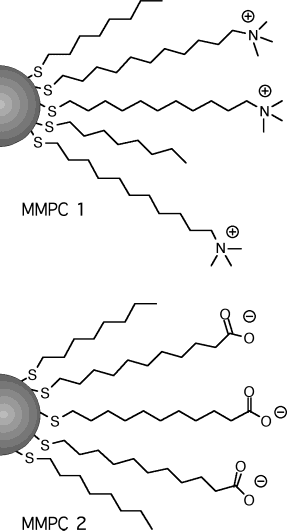
\includegraphics[width=0.2\textwidth]{./img/GoodmanNPs.png}%
	}\qquad\qquad%
	\subfloat[]{%
		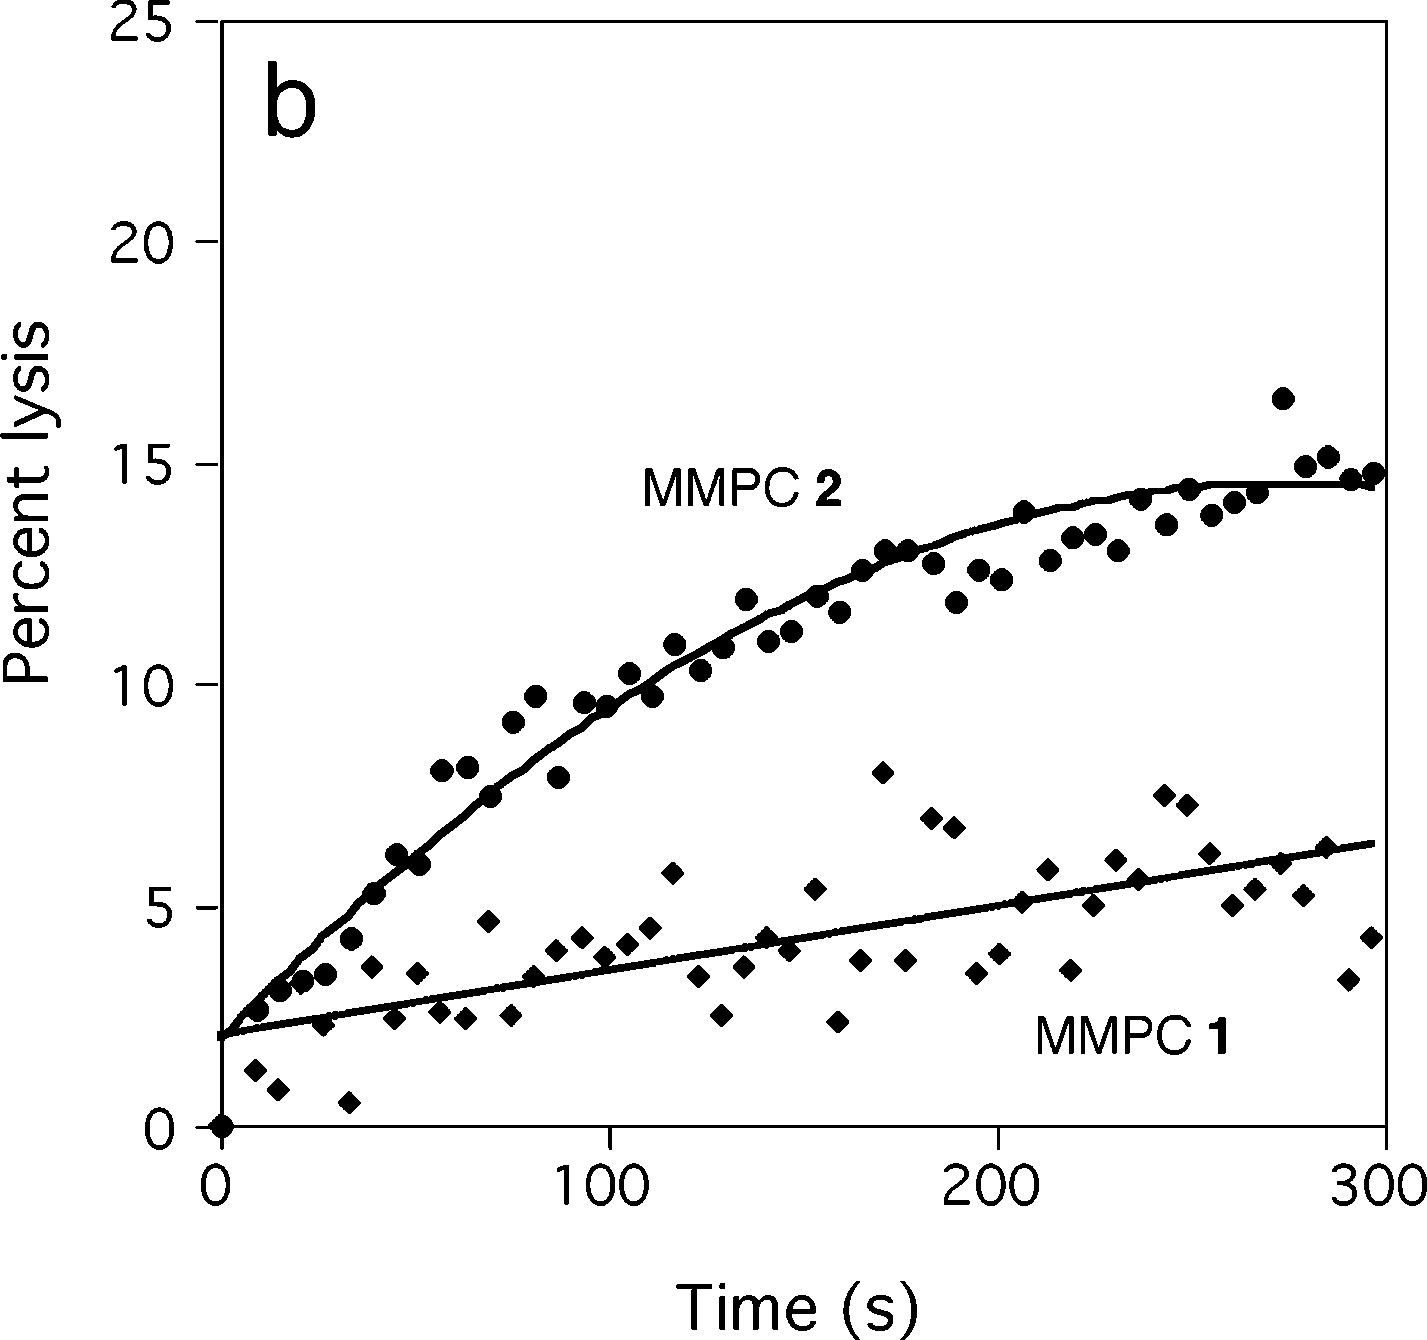
\includegraphics[width=0.4\textwidth]{./img/lysis.png}%
	}%
	\caption{Left: \acp{AuNP} functionalized by a monolayer of neutral and positively charged (MMPC $1$) or negatively charged (MMPC $2$) ligands. Right: Comparison of MMPC $1$ and $2$ in disrupting vesicles made of neutral lipids. In this kind of essays, the disruptive power of the \acp{NP} is quantified by the amount of fluorescent dye that is released from the vesicles. Taken from \cite{Goodman2004}.}%
	\label{fig:goodman}
\end{figure}

More recently, Van Lehn \etal{} \cite{VanLehn2013} have demonstrated via confocal microscopy images, shown in 
figure~(\ref{fig:fluorescent}), that anionic \acp{AuNP} can stably bind to the lipid membrane in a 
non--destructive manner and moreover that they can passively diffuse inside a multilamellar vesicle made of 
zwitterionic lipids. In this experiment \acp{AuNP} were labelled with the red fluorescent BODIPY dye and solved in 
a water solution with the multilamellar vesicle and the green fluorescent calcein dye that does not passively 
diffuse through lipid bilayers.
\begin{figure}[!ht]
	\centering
	\subfloat[calcein fluorescence]{%
		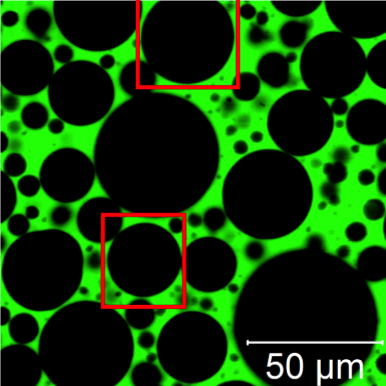
\includegraphics[width=0.28\textwidth]{./img/Calcein.png}%
	}\qquad\qquad\qquad%
	\subfloat[BODIPY fluorescence]{%
		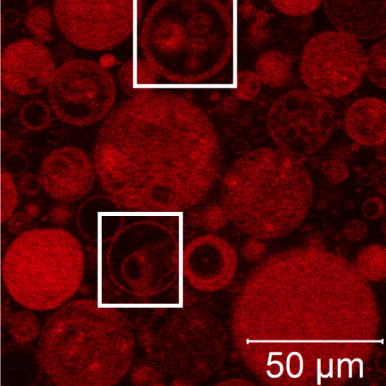
\includegraphics[width=0.28\textwidth]{./img/BODIPY.png}%
	}%
	\caption{Confocal microscopy images of BODIPY--labeled anionic \acp{AuNP} in a solution with multilamellar single--component zwitterionic lipid vesicles and the membrane impermeable dye calcein. Green fluorescence from calcein, left image, was only observed from the vesicle exterior. This means that no vesicles has been destroyed since the calcein can penetrate the vesicle interior only if pores are formed in the lipid membrane. Indicating that anionic \acs{AuNP} do not induce pore formation. BODIPY red fluorescence, right image, was localized to both interior and exterior membranes of the multilamellar vesicles, with a noticeably stronger fluorescence at the interior respect to the background. This suggest a preferential bilayer--\acs{AuNP} interaction and that the \acp{AuNP} can passively diffuse through the lipid membrane in a non--destructive manner. Taken from \cite{VanLehn2013}.}%
	\label{fig:fluorescent}
\end{figure}

In another recent work, Tatur \etal{} \cite{Maccarini2013}, made a neutron reflectometry experiment on a floating 
zwitterionic lipid bilayer in presence of \acp{AuNP} functionalized with both anionic and cationic ligands. 
Studying the structural deformation of the bilayer they found that cationic \acp{NP} are overall more toxic then 
the anionic ones. They found that the latter can passively penetrate into the hydrophobic region of the membrane 
in a non destructive manner for wide range of temperatures under the liquid--gel transition. Above the liquid--gel 
transition, instead, they observed that more and more cationic \acp{NP} can permanently penetrate inside the 
membrane leading to a gradual destabilization of its structure, depending on the quantity of inserted \acp{AuNP}. 
On the contrary, the anionic \acp{AuNP} do not have the tendency to penetrate inside the lipid membrane. Rather, 
they interact with its surface strongly dehydrating the floating bilayer. Clearly these results are in contrast 
with the confocal microscopy observation reported in Van Lehn \etal{} \cite{VanLehn2013} and the observation of 
Goodman \etal{} \cite{Goodman2004}. Hence the importance to perform \ac{MD} simulations to investigate the 
molecular processes involved in the \ac{NP}--membrane interaction.

Other physico--chemical characteristics of the \ac{NP} ligand shell affect the \ac{NP}--membrane interaction. On 
top of all, the hydrophobic character of the ligand shell is believed to play a major role. Moreover, what is most 
intriguing and unexplained is the effect of the ligand composition and surface arrangement on the 
\ac{NP}--membrane interaction. To date, neither the poration process, nor the binding process, nor the effects of 
ligands with different degrees of hydrophobicity have been described at molecular level, hindering the design of 
\acp{NP} with target--specific ligand composition.

\section{state of the art of the computational studies of aunp--lipid membrane interactions}
Van Lehn \etal{} have published a computational work \cite{VanLehn2013} concerning the way anionic \acp{AuNP} 
penetrate cell membrane. They studied the influence of the size and surface composition of functionalized 
\acp{AuNP} on the internalization pathway into the cells in addition to the steps through which the process 
evolves. They used both a thermodynamic--based model and experiments, see figure~(\ref{fig:fluorescent}), to test 
the hypothesis that the first step in cell penetration is the fusion of the \acp{AuNP} with lipid bilayers, the 
process being driven by the hydrophobic effect. The hypothesized mechanism relies on the capability of the ligands 
on the \ac{NP} surface to ``snorkel'' the charged end groups to the aqueous environment thus exposing a greater 
hydrophobic area to the bilayer core. Van Lehn \etal{} conclude that the process is size--dependent rather than 
morphology--dependent and that there exists a critical diameter, dependent on the coating composition, above which 
fusion with the lipid bilayer becomes unfavorable.

Heikkilä \etal{} in \cite{Heikkila2014} demonstrated, by \ac{MD} simulations, that anionic \acp{AuNP} can adsorb 
at the surface of neutral lipid membranes. The limited time scale of the simulations performed in their work, 
which is based on an atomistic \ac{FF} (see chapter~\ref{chap:EmpiricalFF}), did not allow to observe and describe 
any penetration of the \ac{NP} into the hydrophobic membrane core. To speed--up the process, Van Lehn \etal{} in 
\cite{VanLehn2014} have considered the interaction between an anionic \ac{AuNP} and a highly curved lipid bilayer, 
observing the fusion between the \ac{NP} and the membrane.

Gkeka \etal{} modelled rigid \cite{Gkeka2013} and \ac{CG} \cite{Gkeka2014} (see chapter~\ref{chap:EmpiricalFF}) 
\acp{NP}, with different arrangements of the charged surface ligands, in the attempt of deriving free energies of 
transfer from the water phase to the membrane interior for \acp{NP} with different degrees of hydrophobicity.

More recently, in order to speed--up the unbiased \ac{MD} simulation and the \ac{NP}--membrane interaction, 
Simonelli \etal{} \cite{simonelliThesis} and \cite{ourPaper}, have developed a \ac{CG} model of the anionic, 
passivated \ac{AuNP} (see chapter~\ref{chap:membraneNP}). The enhancement of the computational performance, thanks 
to the \ac{CG} model, allowed to derive, via unbiased \ac{MD} simulations, the molecular mechanism associated to 
the interaction between the \ac{NP} and a planar model biological membrane. Furthermore they found that the 
\ac{NP}--membrane interaction depends on the surface arrangements of the \ac{NP} ligands.

% \section{state of the art of the free energy calculations on lipid membrane solutes translocation}
% Free energy calculations refers to the possibility, via advanced sampling methods, to obtain thermodynamic results of processes or transitions between two metastable states that have low probability to occur in an \textit{unbiased} \ac{MD} simulation at a certain temperature. As better explained in chapter~\ref{chap:methods} advanced sampling methods force --- via the introduction of a bias force --- the sampling of the non--accessible phase space. Advanced sampling methods allow to accelerate rare events, and so simulate them within accessible time scales, and to provide a quantitative description of the \ac{FES} in the region of interest of the phase space. A simple example involving lipid membranes is the ion translocation through the bilayer from the water phase: the advanced sampling methods allow for the extremely unlikely process to occur and, as accurately as possible, for the estimation of the free energy profile. To do this a \ac{CV} or an order parameter, a variable or a set of variables that describes the process of interest, are necessary in order to integrate out the other, supposed, unnecessary \ac{DOF}. In the above example and in those cases in which the process of interest is a solute translocation through a lipid bilayer, the most intuitive and commonly--used \ac{CV} is the distance between the \ac{COM} of the solute and the \ac{COM} of the lipid membrane along the bilayer normal. Unfortunately, in most cases this \ac{CV} is the origin of some sampling error and a non correct estimation of the \ac{FES}, as outline in a review by by Neale and Pomès \cite{Neale2016}.

% In the following we summarize the main concepts useful for this thesis work, for a more comprehensive discussion the reader is addressed to the review by Neale and Pomès \cite{Neale2016}.

%The sampling errors, which often are systematic, arise when large free energy barriers in orthogonal degrees of freedom, also called hidden free energy barriers, trap the sampling in a undesired metastable states. In the lipid membrane solutes translocation, the common hidden energy barriers are due to deformations of one or both leaflets. There are two main kind of deformations: an invagination of the bilayer around the solute, as shown in figure~(\ref{fig:hfes}) or a deformation of one or both leaflets due to the interaction between the charged lipid heads and the charged solute groups (and its hydration shell), as shown in figure~(\ref{fig:invaginatino}). In the last effect, the solute, bringing water and lipid head groups of one or both leaflet can create a membrane defect that can lead to a water pore formation. %The invagination or the deformation of one or both leaflets of the bilayer upon solute penetration implies that the free energy cost of desolvating ionic solutes exceeds the cost of bilayer deformation and hence that the magnitude of the free energy barrier of the entrance process depends to a large extent on the bilayer's thickness and bending modulus.
% \begin{figure}[ht!]
% 	\centering
% 	\subfloat[]{%
% 		\begin{minipage}[c][1\width]{0.4\textwidth}%
% 			\centering%
% 			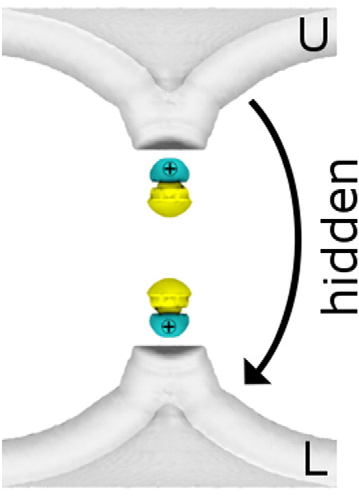
\includegraphics[width=0.6\textwidth]{./img/HFES.png}%
% 			\label{fig:hfes}%
% 		\end{minipage}%
% 	}\qquad%
% 	\subfloat[]{%
% 		\begin{minipage}[c][1\width]{0.4\textwidth}%
% 			\centering%
% 			
\includegraphics[width=\textwidth]{./img/invagination.png}%
% 			\label{fig:invaginatino}%
% 		\end{minipage}%
% 	}%
% 	\caption{Bilayer distortion and hidden free energy barriers underlying systematic sampling errors in free energy calculations. (a) Example of both leaflets trailing towards the bilayer core due the translocating solute. In gray the phosphorus atoms behind the solute and yellow hydrophobic and cyan hydrophilic moieties of the solute. The curved arrow indicate the hidden energy barriers. (b) Example of a possible invagination of the lipid membrane around the solute; the \acs{COM} of the solute and the lipid bilayer coincide but the solute is still in the water phase. Taken from \cite{Neale2016}.}%
% \end{figure}

%The invagination effect, that can be caused also by a sufficiently large bilayer, can cause false associations between the \ac{CV} and the state of the system. As shown in figure~(\ref{fig:invaginatino}) defining the \ac{CV} as the distance between the \ac{COM} of the solute and the bilayer, $|z|$, a solute at $|z| = 0$ may not for a direct contact with the core of the bilayer, there by sampling an irrelevant region of phase space and yielding a free energy profile with no real predictive value.

%The main force acting on a charged solute embedded near the bilayer center is largely determined by the presence of a defect that brings water and lipid head groups of one or both leaflets into the bilayer's hydrophobic core. Therefore, the extent to which the free energy profile of translocation is affected by sampling errors depends on the free energy of defect formation for a given \ac{FF}. Unexpectedly, the likelihood of forming such defects, which is intricately tied to the bilayer's bending modulus, can depend on the way the non--bonded interactions are modelled. In the common case of a Lennard--Jones potential, it depend, therefor, in the used truncation methods.

%By far the most commonly used \ac{CV} in free energy simulations of solute--bilayer interactions is the distance between the \ac{COM} of the solute and that of the bilayer along the bilayer normal. The existence of persistent systematic sampling errors, as seen above, demonstrates that this commonly--used order parameter is inadequate for many free energy calculations. However, the selection of the optimal \acp{CV} set is a challenging problem that deserves a more appropriate studies for understand if the set of \acp{CV} are useful to describe the process and how it impact the computational performance of the simulation: a incredible perfect set of \acp{CV} that slow down the simulation can not be useful. For this and for a comparison between the results obtained in \cite{ourPaper} to be made, for this thesis work, we have chosen to not change the selected \ac{CV}, based on the distance between the \ac{COM} of the solute and the membrane along the bilayer normal.

\section{objectives}
In the previous paragraphs we have highlighted two main challenges related to the study of charged metal 
\ac{NP}--membrane interactions. The first consists in the difficulty to experimentally achieve a molecular--level 
description of the \ac{NP}--membrane interaction. This issue could in principle be addressed computationally, but 
the second difficulty soon kicks in --- at computational level the \ac{NP}--membrane interaction is a 
``\textit{slow}'' process, and it is not trivial to achieve the optimum compromise between the model reliability 
and computational efficiency.

Here we list the three main objectives of this thesis:
\begin{enumerate}[label=\itshape\roman*.]
	\item Is the binding of anionic \acp{NP} to zwitterionic lipid membranes favorable from an energetic point of 
	view? If it is, can we use \ac{MD} simulations to reveal the molecular mechanisms that lead to
	\ac{NP}--membrane binding, and can we make quantitative predictions about the strength of the 
	\ac{NP}--membrane 
	interactions?%
	\item The \ac{NP}--membrane interaction is driven by two main physical causes: \textit{a.} the hydrophobic 
	effect, that favors the hydrophobic contacts between the \ac{NP} and the membrane, and \textit{b.} 
	electrostatic interactions, that favor the contact between the anionic \ac{NP} ligands and the neutral, but 
	polar, heads of the lipid molecules. The role played by electrostatics is important, but electrostatic 
	interactions are not always properly taken into account by the classical interaction models used in 
	biomolecular simulations. All--atom models typically include the description of long--range electrostatics and 
	the molecular orientational polarizability, but are extremely expensive from a computational point of view. 
	\ac{CG} models, on the contrary, are computationally efficient but often inaccurate at the description of the 
	interaction between charged or polar molecules. Our aim is to compare these different approaches and suggest 
	what model allows for the best compromise between computational efficiency and reliability.%
	\item In presence of mixed--ligand shells, can the surface arrangement of ligands influence the \ac{NP} 
	interaction with the membrane? Our objective is to consider \acp{NP} passivated with a mixed shell of 
	hydrophobic and anionic ligands. We will look at \acp{NP} in which the two kinds of ligands have an ordered 
	(striped--like) arrangement of the two ligands, and \acp{NP} with a random ligand arrangement. In both cases 
	we will characterize the \ac{NP}--membrane interaction mechanism and compare the \ac{NP}--membrane binding 
	energies of the two samples.%
\end{enumerate}

\section{contents overview}
In this thesis we characterize the interactions between an anionic, ligand--protected \ac{AuNP} and a model lipid 
membrane by means of \ac{MD} simulations and an enhanced sampling method, called metadynamics. Both \ac{MD} and 
metadynamics main features are described in chapter~\ref{chap:methods}.

The choice of the appropriate model of inter--particle interactions to feed the \ac{MD} method depends on the 
typical time and length scales of the system of interest. The stages of the \ac{NP}--membrane interaction --- from 
the water phase to the \ac{NP} embedded into the lipid membrane  --- take place on time scales of at least tens of 
microseconds. In terms of length scales, the size of the membrane patch to be considered in our simulations needs 
to be as large as $10$~nm at least, in order to be able to accommodate a \ac{NP} which metal core has a diameter 
of about $2$~nm. These time and length scales are not compatible with the use of an atomistic \ac{FF}, that is, a 
model interaction potential describing the interactions between all the atoms in the system. We thus adopted a 
\ac{CG} approach, based on the idea that groups of atoms (e.g. the charged terminal group of an anionic ligand, or 
the polar head of a lipid) can be represented by single particles. A general introduction and features about 
\ac{FF}, the advantages (and disadvantages) of a \ac{CG} \ac{FF} over an atomistic one and a detailed description 
of the \ac{CG} \ac{FF} that we will use are described in the first part of chapter~\ref{chap:EmpiricalFF}. Since 
we are interested in improving the treatment of the electrostatic interaction, in the second part of 
chapter~\ref{chap:EmpiricalFF} we present two methods to efficiently and accurately treat the electrostatic 
interaction: the \ac{ESM} and the \ac{PME} method.

In chapter~\ref{chap:software} we present a general overview of the software tools used in this work. Moreover, 
some computational tricks and tips used to improve the computational performance of our \ac{MD} runs are 
presented. The main one is the use of an hardware (GPU) accelerated framework to off--load the non--bonded 
calculations and achieve a speed--up of about $2-4$ times with respect to non accelerated simulation.

In chapter~\ref{chap:membraneNP} we present the main properties of the \ac{CG} model of the biological lipid 
membrane and the \ac{CG} model of the anionic, ligand--passivated \ac{AuNP} developed by Simonelli \etal{} 
\cite{simonelliThesis} and \cite{ourPaper}. Then, the step--by--step pathway of the \ac{NP}--membrane interaction 
--- from \ac{NP} adsorbing at the membrane surface to the embedding of the \ac{NP} into the membrane core --- is 
summarized.

In chapter~\ref{chap:results} we present our results. We conclude that: \textit{i.} Anionic \acp{AuNP} can stably 
bind to the hydrophobic core of neutral lipid membranes; \textit{ii.} It is necessary to include long range 
electrostatic interactions and use a water model that allows for the explicit electrostatic screening to achieve, 
at \ac{CG} level, results quantitatively in agreement with the higher resolution atomistic model; \textit{iii.} 
Different ligand arrangements on the surface of the \ac{NP} can significantly affect the energies of binding of 
the \ac{NP} to the membrane.

Conclusions and perspectives are reported in chapter~\ref{chap:conclusions}.

%restore toc configuration
\restoretoc
\endgroup

%*--------------------------------------*
%|***************INDEXPAGE**************|
%*--------------------------------------*
\tableofcontents

%\restoregeometry

\clearscrheadfoot
\pagestyle{scrheadings}
\rohead{\rightmark\qquad\pagemark}
\lehead{\pagemark\qquad\leftmark}

\renewcommand{\sectionmark}[1]{\markright{\spacedlowsmallcaps{\textcolor{gray}{\thesection\ #1}}\normalfont}}
\renewcommand{\chaptermark}[1]{\markleft{\normalfont\spacedlowsmallcaps{\textcolor{gray}{\thechapter\ #1}}\normalfont}}

\mainmatter

% !TEX root = ./../main.tex
\chapter{Introduction to Molecular Dynamics}
For macroscopic bodies, the motion of a system in time and space is governed by the classical equations of 
motion, say Newton’s laws, while reducing time and space scales, quantum mechanics kicks in. Despite the latter 
statement, classical laws of motion have proved to be a good approximation also at the molecular level, as long 
as atoms are massive enough.

In order to predict the time evolution of a complete system, such as the biomolecular system we will treat in 
this thesis, Newton’s equations of motion need to be integrated numerically. The necessity of a numerical 
integration arises from the complexity of the interactions involved in realistic systems, often nonlinear 
functions of positions and momenta of the particles, which makes it impossible to obtain an analytical solution 
for the equations of motion.

In the first part of this Chapter the laws of classical and statistical mechanics will be briefly summarized.
Then we will introduce the computational \acf{MD} method and analyze the main aspects of this technique with some 
details about the \textit{empirical} \ac{FF}: the container of system model and parameters under study. This 
includes the way to consider and treat the inter--particle interactions at \ac{MD} level. Then, coarse--graining 
procedure are introduced, with particular attention to the \martini \ac{FF}, the main \ac{FF} used in this thesis 
work. Lastly advanced sampling techniques are explained: the \textit{Umbrella Sampling} and 
\textit{Metadynamics}. This introductory Chapter are based on the books of Tuckerman \cite{Tuckerman}, Leach 
\cite{Leach}, Frenkel and Smit \cite{Frenkel} and Allen and Tildesley \cite{Allen} to which the reader is 
addressed for a more complete discussion.

\section{Review of classical mechanics}
Let us consider a system of $N$ particles with mass $m_i$ and coordinates $\vec r_1,\dots,\vec r_N$. According 
to the Newton's second low each particle will experience a total force $\vec F_i$ such that
\begin{equation}
	m_i \ddot{\vec{r}}_i = \vec F_i(\vec r_1,\dots,\vec r_N)
	\label{eq:newtonLaw}
\end{equation}
The total force on each particle is defined as
\begin{equation*}
	\vec F_i(\vec r_1,\dots,\vec r_N) = \vec{f}_i^{\ (e)}(\vec r_i) + \sum_{i\ne j}^N \vec{f}_{ij}^{\ (i)}(\vec r_i - \vec r_j )
\end{equation*}
where $\vec{f}_i^{\ (e)}$ is an external force acting on particle $i$ and $\vec{f}_{ij}^{\ (i)}$, which in general
depends only on distance between particle $i$ and $j$, is the inter-particle force that $i$ exerts on $j$ and
\textit{vice-versa}. Equations~\eqref{eq:newtonLaw} are refereed to as \textit{the equations of motion} of the
system; integrating them, with the sets of the \textit{initial conditions} at start time 
$t_0$ $\vec r_1(t_0),\dots,\vec r_N(t_0)$ and $\dot{\vec{r}}_1(t_0),\dots,\dot{\vec{r}}_N(t_0)$, the positions 
and the velocities of all the particles in the system at any time are known.

Another way to write the equations of motion is to use particles momenta $\vec p_i = m_i \dot{\vec{r}}_i$ and then
the equations~\eqref{eq:newtonLaw} become
\begin{equation}
	\frac{d\vec p_i}{dt} = \vec F_i(\vec r_1,\dots,\vec r_N)
	\label{eq:newtonLawMom}
\end{equation}
The full set of $6N$ functions $(\vec r_1(t),\dots,\vec r_N(t),\vec p_1(t),\dots,\vec p_N)$ gives us a full
description of the dynamics of the $N$--particle system. The set of functions above can be arranged in an ordered 
$6N$--dimensional vector
\begin{equation}
	\vec x(t) = (\vec r_1(t),\dots,\vec r_N(t),\vec p_1(t),\dots,\vec p_N)
	\label{eq:phSpaceVector}
\end{equation}
called \textit{phase space vector} or the \textit{microstate} of the system at time $t$. All the possible
microstates of a system generate a $6N$--dimensional space called \textit{phase space} of the system, indicated 
with $\Omega$. Thus $\vec x(t)$ describes a particular trajectory in the phase space, i.e. the system evolution 
is the motion of a phase space point. For simplicity of notation let us introduce also the ordered vectors 
$\vec r = (\vec r_1, \dots, \vec r_N)$, $\dot{\vec r} = (\dot{\vec{r}}_1,\dots,\dot{\vec{r}}_N)$ and 
$\vec p = (\vec p_1, \dots, \vec p_N)$ which are the coordinates, velocities and momenta off all particles.

Let us suppose that all the forces acting on the $N$--particle system are conservative; this means that it must
exist a scalar function $U = U(\vec r)$ called \ac{PEF}, such that
\begin{equation}
	\vec F(\vec r) = -\partial_{r_i} U(\vec r)\ \hat e_i = -\vec\nabla_{\vec r} U(\vec r)
	\label{eq:pefForces}
\end{equation}
where $\vec F = (\vec F_1,\dots, \vec F_N)$. Thus we have only to know the \ac{PEF} of the system at any time and 
the initial conditions to solve Newton's laws.

The kinetic energy of the system is defined as
\begin{equation}
	K(\dot{\vec r}) = \sum_{i=0}^{N}\frac{1}{2}m_i \dot{\vec r}_i\cdot \dot{\vec r}_i
	\label{eq:kinetic}
\end{equation}

If the system is conservative we can define a scalar function, called \textit{Lagrangian} of the system
\begin{equation}
	\mathcal{L}(\vec r,\dot{\vec r}) = K(\dot{\vec r}) - U(\vec r)
	\label{eq:lagrangian}
\end{equation}
such that
\begin{equation}
	\frac{d}{dt}\left ( \frac{\partial \mathcal{L}}{\partial \dot r_{i}}\right ) - \frac{\partial\mathcal{L}}{\partial r_{i}} = 0
	\label{eq:EulerLagrange}
\end{equation}
These set of $3N$ equations are called \textit{Euler--Lagrange equations of motion}. It is easy to show that 
substituting the definition of $\mathcal{L}$ we obtain the Newton's second law. The Euler--Lagrange equations are 
a sort of generator of the equations of motion.

Using the definition of $\mathcal{L}$ \eqref{eq:lagrangian} we have
\begin{equation}
	p_i = \frac{\partial\mathcal{L}}{\partial \dot r_i} = m_i\dot r_i
	\label{eq:momentaLagrangian}
\end{equation}
thus we can express particle velocities as a function of particle momenta. Equations~\eqref{eq:kinetic}
and~\eqref{eq:momentaLagrangian} let us to express the kinetic energy in the form
\begin{equation}
	K(\vec p) = \sum_{i=0}^N \frac{\vec p_i \cdot \vec p_i}{2m_i}
	\label{eq:kineticP}
\end{equation}

To describe the system we can define another scalar function, called \textit{Hamiltonian} of the system
\begin{equation*}
	\mathcal{H}(\vec r, \vec p) = \sum_{i=0}^N \vec p_i \cdot \dot{\vec r}_i(\vec p_i) - \mathcal{L}(\vec r, \dot{\vec r}(\vec p))
\end{equation*}
Substituting~\eqref{eq:lagrangian} and using~\eqref{eq:kineticP} the Hamiltonian of the system is nothing that
\begin{equation}
	\mathcal{H}(\vec r, \vec p) = K(\vec p) + U(\vec r)
	\label{eq:hamiltonian}
\end{equation}
or \textit{the total energy of the system}. To obtain the equations of motion we have to solve \textit{Hamilton's equations}
\begin{equation}
	\begin{aligned}
		\dot r_i &=& &\frac{\partial\mathcal{H}}{\partial p_{i}} \\
		\dot p_i &=&-&\frac{\partial\mathcal{H}}{\partial r_{i}}
	\end{aligned}
	\label{eq:eqhamilton}
\end{equation}
Describing the system with the Hamiltonian formalism, in some cases, is more useful than Lagrangian one, first of
all because the Hamiltonian of a system is directly related to a well know physical quantity, the total energy.

\section{Review of statistical mechanics}
\label{sec:statmec}
Using the picture of the classical mechanics described above we have a good and sophisticated machinery that 
allows us, knowing some information about the system in exam, i.e. initial positions and velocities of all 
particles and their interactions, to completely solve the equations of motion in order to get the dynamics of the 
system at every time. So classical mechanics encodes all the information about the \textit{microscopic} view of a 
system and, in principle, we can extract all the information we want about the \textit{macroscopic} proprieties 
of such system. The main task of this process is to obtain the thermodynamics proprieties of a system 
(temperature, pressure and so on) from the complete sets of positions and velocities of all particles and thus it 
is necessary to have a link between microscopic and macroscopic world.

The solution of that problem comes from \textit{statistical mechanics} developed, principally, by Boltzmann and 
Gibbs. Statistical mechanics involves all the rules and methods through which the microscopic and macroscopic 
worlds are related to each other. This provides also a rigorous derivation of thermodynamics from the microscopic 
proprieties: without that thermodynamics would be only a phenomenological theory. The first step to the solution 
of the problem is to recognize that \textit{a macroscopic observable of a system does not strongly depend on the 
complete dynamics of each particle in the system, but rather on an average that cancels out all the details of 
the microscopic features}. This it is intuitively true. We can think to set up an experiment with a system in a 
specific microscopic state that corresponds to a macroscopic state. Certainly we can do the contrary and for sure 
we wont find the same microscopic state. Then we can iterate the experiment and we will find that for a specific 
macroscopic state of a system there exists a number of microscopic states that yield to the same properties.

The most important concept that makes this idea practicable is the \textit{statistical ensemble}. Based on the 
previous considerations, a general definition of an ensemble is \textit{a collection of systems subject to a set 
of common interactions and sharing the same macroscopic properties}. This concept lays the foundations of 
thermodynamics and suggests a procedure to compute many macroscopic observables. In more details a 
$N$--particle system in a specific microscopic state is described by its microstate $\vec x$, then \textit{an 
ensemble is a set of points in the phase space that are subject to the constraint to be part of the ensemble 
itself}. Each system evolves in time with the equations of motion, so the time evolution of an ensemble is 
described by the flow of a set of points in the phase space according to the classical mechanics.

Once an ensemble is defined we are able to compute, at every time, the macroscopic observables simply averaging 
over all systems in the ensemble. To do this we have to know, at every time, which microstates of the phase space 
are part of the ensemble. For this purpose we define the \textit{ensemble distribution function} 
$\tilde\rho = \tilde\rho(\vec x,t)$. Let $dx = dr_1\cdots dr_{3N} dp_1 \cdots dp_{3N}$ the infinitesimal phase 
space volume, then
\begin{equation*}
	\frac{1}{\mathcal{N}}\tilde\rho(\vec x, t)\ dx = \rho(\vec x, t)\ dx ????
\end{equation*}
where $\mathcal{N}$ is the total number of microstates in the ensemble. $\rho(\vec x, t)dx$ can be interpreted as 
the probability to find in the ensemble a system with microstate $\vec x$ at a time $t$ and $\rho(\vec x, t)$ is 
the more convenient normalized distribution function. For definition of probability density must be
\begin{equation*}
	\int_{\Omega} \rho(\vec x, t)\ dx = 1, \qquad \rho(\vec x, t) \ge 0
\end{equation*}

Giving the ensemble distribution function, the ensemble average of an observable $A=A(\vec x)$, at every time, is 
defined as
\begin{equation*}
	\ave{A}(t) = \int_\Omega A(\vec x)\rho(\vec x, t)\ dx
\end{equation*}
For an ensemble at thermodynamic equilibrium the macroscopic state is fixed and so, if $A$ is an equilibrium 
observable, it must be time--independent. Thus, it can be shown \cite{Tuckerman} that exist a scalar function of 
the Hamiltonian $\mathit{f}(\mathcal{H}(\vec x))$ such that the time--independent ensemble average of the 
equilibrium observable $A$ can be expressed as 
\begin{equation*}
	\ave{A} = \frac{1}{\mathcal{Z}} \int_\Omega A(\vec x, t) \mathit{f}(\mathcal{H}(\vec x))\ dx
\end{equation*}
where $\mathcal{Z}$, known as \textit{partition function}, is specific for the ensemble in exam and it is defined 
as follow
\begin{equation*}
	\mathcal{Z} = \int_\Omega \mathit{f}(\mathcal{H}(\vec x))\ dx
\end{equation*}

In order to compute the partition function we need to specify the thermodynamic observables, called 
\textit{control variables}, that characterize the ensemble itself. By definition of an ensemble at thermodynamic 
equilibrium those control variables must be constant in time. The main ensembles used in statistical mechanics 
and the related control variables are summarized as follow
\begin{itemize}
	\item \textit{microcanonical ensemble}: constant--$NVE$
	\item \textit{canonical ensemble}: constant--$NVT$
	\item \textit{isothermal--isobaric ensemble}: constant--$NpT$
	\item \textit{grand--canonical ensemble}: constant--$\mu pT$
\end{itemize}
The averages computed in different ensembles are equivalent in the so called \textit{thermodynamic limit}: this 
is the \textit{equivalence of ensembles}. Thus, it must be possible to change from one ensemble to another 
leaving averages unchanged.

We have defined ensemble averages and how to compute them but we need also a link between statistical averages 
and the experimental values. When we measure a macroscopic observable $A$ we prepare an experiment with 
\textit{only one} system in a specific macroscopic state and we study its evolution in time. $A$ is a function of 
time and phase space vector and it fluctuates over time due to particle interactions. The measurement itself 
requires long time intervals compared to microscopic time scales, thus when we measure an observable we take an 
\textit{average over time}. If, in principle, the time for average is infinity then we have the ``real'' mean 
value of the observable
\begin{equation*}
	\overline{A} = \lim_{\tau\to +\infty}\frac{1}{\tau}\int_{t_0}^\tau A(\vec x_t)\ dt
\end{equation*}
In order for a comparison to be made, an identity between ensemble and time averages must be established.
This link is provided by the \textit{ergodic theorem} and the \textit{ergodic hypothesis}. A system is said to be 
ergodic if, over a long period of time, all the microstates in the phase space with the same energy are 
accessible with the same probability. Then the ergodic theorem says that, if the system is ergodic, the time and 
ensemble averages are equal \textit{almost everywhere} in the phase space. So we can write the follow identity
\begin{equation}
	\overline{A} = \lim_{\tau\to +\infty}\frac{1}{\tau}\int_{t_0}^\tau A(\vec x(t))\ dt = \int_\Omega A(\vec x)\rho(\vec x, t)\ dx = \ave{A}(t)
	\label{eq:ergotic}
\end{equation}

For biomolecular applications the most important ensembles are the microcanonical and the isothermal--isobaric. 
In the following we will describe them briefly with particular attention to the isothermal--isobaric ensemble, 
the most relevant for this thesis work.

\subsection{Microcanonical ensemble}
The microcanonical ensemble is composed of the systems whose number of particles ($N$), volume ($V$) and energy 
($E$) are constant. Due to the constant energy it describes a Hamiltonian system for which
\begin{equation*}
	\mathcal{H}(\vec x) = E
\end{equation*}
this let us to define the partition function as follow
\begin{equation}
	\mathcal{Z}_{NVE} = \frac{1}{N!h^{3N}}\int_\Omega \delta(\mathcal{H}(\vec x) - E)\ dx
	\label{eq:micropartition}
\end{equation}
where the normalization factor $N!$ takes into account the particles indistinguishability and $h^{3N}$ is for 
compatibility of statistical mechanics with quantum mechanics: it comes from Heisenberg’s uncertainty principle 
and it is the smallest phase space volume element. The right thermodynamic potential, i.e. the constant of 
motion, to obtain all the macroscopic observables is the entropy $S$ given by
\begin{equation*}
	S = k_B \ln \mathcal{Z}_{NVE}
\end{equation*}
where $k_B = 1.3806505(24) \cdot 10^{-23}$~J/K is the Boltzmann constant. The other thermodynamic quantities can 
be obtained by
\begin{equation*}
	\frac{1}{T} = \left ( \frac{\partial S}{\partial E}\right )_{NV} \qquad \frac{p}{T} = \left ( \frac{\partial S}{\partial V}\right )_{NE} \qquad \frac{\mu}{T} = \left ( \frac{\partial S}{\partial N}\right )_{VE}
\end{equation*}

The link between microscopic functions of phase space points and macroscopic observables, like kinetic energy or 
pressure, is provided by the \textit{classical virial theorem} which states that
\begin{equation}
	\ave{x_i\frac{\partial\mathcal{H}}{\partial x_k}} = k_B T \delta_{ik}
	\label{eq:virial}
\end{equation}
where $x_i$ is some phase space variable.
% often the virial theorem is written in a slightly different form
% \begin{equation}
% 	\ave{K} = - \frac{1}{2}\sum_{i=1}^{3N} \ave{F_ir_i}
% \end{equation}
% where $\ave{K}$ is the average kinetic energy, not necessary at equilibrium and $F_i$ is the total forces acting on particle $i$. Both are valid even if the system is not at the equilibrium.

\paragraph{\textbf{Kinetic energy}} Since a system in a microcanonical ensemble is defined to be Hamiltonian, 
from equations~\eqref{eq:hamiltonian} and~\eqref{eq:kineticP} according to the virial theorem with the choice 
$x_i = p_{i}$ we obtain
\begin{equation*}
	\ave{\frac{p^2_{i}}{m_i}} = k_bT
\end{equation*}
then summing both side over all particles and over the three coordinates we obtain the average kinetic energy at 
equilibrium
\begin{equation}
	\ave{K} = \ave{ \sum_{i=1}^{N}\sum_{\alpha=1}^{3}\frac{p_{i+\alpha}^2}{2m_i} } = \ave{\sum_{i=1}^{N}\frac{\vec p_i\cdot \vec p_i}{2m_i}} = \frac{3}{2}Nk_B T
	\label{eq:kineticT}
\end{equation}
this is like the well know equipartition theorem in which $3N$ is the number of \ac{DOF}.

\paragraph{\textbf{Pressure}} Choosing $x_i = r_i$ in equation~\eqref{eq:virial} and summing both side over all 
particles and substituting equations~\eqref{eq:eqhamilton} and~\eqref{eq:kineticT}, we obtain
\begin{equation*}
	W = \ave{\sum_{i=1}^{3N} r_i\dot p_i} = -3Nk_B T = - 2 \ave{K}
\end{equation*}
the quantity $W$ is often called \textit{virial}. For a $N$--particle non--interacting system it is well known 
that $pV = Nk_B T$ thus the virial is $W = -3pV$. For a real interacting system we need to include in the virial 
the contribution due to the inter--particles interactions $U(\vec r_1,\dots,\vec r_N)$, thus the virial 
becomes\footnote{We assume that the inter--particles interactions are pairwise addictive which they depends only 
on distances between particles $i$ and $j$.}
\begin{equation*}
	W = -3pV + \ave{ \sum_{i=1}^N\sum_{j=i+1}^Nr_{ij}f_{ij} } = - 2 \ave{K}
\end{equation*}
where $r_{ij}$ and $f_{ij}$ are the distance and force between particles $i$ and $j$. Thus the pressure of the 
system is given by
\begin{equation*}
	p = \frac{1}{3V}\left (2 \ave{K} + \ave{ \sum_{i=1}^N\sum_{j=i+1}^Nr_{ij}f_{ij} } \right )	
\end{equation*}
The instantaneous pressure in terms of the phase space points $\vec x(t)$ is obtained substituting 
equation~\eqref{eq:kineticT} and getting the quantity in the average bracket, so
\begin{equation}
	p(\vec x_t) = \frac{1}{3V} \sum_{i=1}^{N} \left ( \frac{\vec p_i \cdot \vec p_i}{m_i} +  \sum_{j=i+1}^Nr_{ij}f_{ij}  \right )
	\label{eq:pressure}
\end{equation}

\subsection{Isothermal--isobaric ensemble}
The isothermal--isobaric ensemble contains those systems with constant particles number ($N$), pressure ($p$) and 
temperature ($T$). This is useful in many chemical, biological and physical systems since their properties are 
reported in conditions of standard temperature and pressure. To maintain the system at constant temperature and 
pressure it is necessary to couple it with an external \textit{temperature bath} and a \textit{pressure bath}. 
The first one can be considered simply a very big system at constant temperature with a high thermal capacity. 
The second can be idealized like a piston connected to the system: it change the volume in order to adjust the 
pressure. The instantaneous work done by the system against the external piston is defined by $pV$, where $V$ is 
the instantaneous system volume. Then we have to correct the Hamiltonian of the system: 
$\mathcal{H}(\vec x) \rightarrow \mathcal{H}(\vec x) + pV$. The partition function is then defined considering 
the Boltzmann ensemble distribution function
\begin{equation}
	\mathcal{Z}_{NPT} = \frac{1}{N!h^{3N}}\int_0^{+\infty}\ dV \ \int_\Omega e^{-\beta(\mathcal{H}(\vec x) + pV)}\ dx
	\label{eq:nptPartition}
\end{equation}
where $\beta^{-1} \equiv k_B T$ and the normalization factor is the same as in 
equation~\eqref{eq:micropartition}. The right thermodynamic potential, i.e. the constant of motion, to obtain the 
other thermodynamic quantities is the Gibbs free energy $G = H - TS$ (where $H$ is the enthalpy) defined by
\begin{equation*}
	G = -k_B T\ln \mathcal{Z}_{NpT}
\end{equation*}
it describes the maximum reversible work that may be performed by the system. The other thermodynamic quantities 
can be obtained by
\begin{equation*}
	\mu = \left ( \frac{\partial G}{\partial N}\right )_{pT} \qquad \ave{V} = \left ( \frac{\partial G}{\partial p}\right )_{NT} \qquad S = \left ( \frac{\partial G}{\partial T}\right )_{Np}
\end{equation*}

For anisotropic systems, volume can undergo different changes in the three Cartesian directories even if external 
pressure is applied isotropically. In these cases it is necessary to take this into account in the partition 
function. The way is to define a matrix formed by the three basis vectors of the system box $\vec a$, $\vec b$ 
and $\vec c$
\begin{equation}
	 \mathbold{H} = 
	\begin{pmatrix}
		a_1 & b_1 & c_1 \\
		a_2 & b_2 & c_2 \\
		a_3 & b_3 & c_3 \\
	\end{pmatrix}
	\label{eq:volumeMatrix}
\end{equation}
so that its volume is $V = \vec a\cdot \vec b\times \vec c = |\det{ \mathbold{H}}|$. The partition function become
\begin{equation*}
	Z_{NpT} = \frac{1}{N!h^{3N}}\int\ d \mathbold{H} \ \int_\Omega \frac{1}{(\det{H})^2} e^{-\beta(\mathcal{H}(\vec x) + p|\det{ \mathbold{H}}|)}\ dx
\end{equation*}
where $\int\ d\mathbold{H}$ is an integral over all nine components of $\mathbold{H}$. Hence, the instantaneous 
pressure can no longer be described by a single quantity. Instead a $3\times 3$ pressure matrix $ \mathbold{P}$ 
is needed. What one find, if the system is isotropically coupled, is that on average, this pressure matrix 
reduces to a diagonal pressure matrix such that
\begin{equation*}
	\text{Tr}\ave{ \mathbold{P}} = 3p
\end{equation*}

%eventualmente vedere se mettere le fluttuazioeni di energia e volume

\section{Molecular Dynamics simulation}
\label{sec:MD}
\acf{MD} is a set of techniques that allow us to prepare a ``computer experiments'' in which solving numerically 
the classical equations of motion of a virtual system we will be able to know its time evolution. Such virtual 
experiment approach has the advantage that many experiments can be set up with different initial conditions 
and/or with different control parameters, such as temperature or pressure. Obviously that experiment is carried 
out using a model that approximates the real system. The main parts of that model are the information required to 
obtain an approximation of the interactions among all system particles, i.e. to compute the \ac{PEF} from which 
the forces are derived by equation~\eqref{eq:pefForces}. Solving the equations of motion with a numerical 
integrator, an \ac{MD} simulation generates a set of phase space vectors, a \textit{trajectory}, at discrete 
times that are multiples of the fundamental time discretization parameter, called \textit{MD time step}; 
$\delta t$. Starting from an initial phase space vector $\vec x(0)$, at each step, the forces are computed from 
the \ac{PEF}. Then the equations of motion are integrated and a new phase space vector $\vec x(\delta t)$ is 
generated, thus a new set of forces is computed and so on. In order to compute time averages we need to 
discretize equation~\eqref{eq:ergotic} so the time integration is substituted with a summation over the collected 
data at certain time step $\Delta \tau = i \delta t$, $i=1,2,3,\dots$. If $i > 1$ only a subset of the collected 
data is used to compute time averages. The formula becomes
\begin{equation}
	\ave{A} = \frac{1}{M}\sum_{n=1}^M A(\vec x(n\Delta \tau))
	\label{eq:MDTimeAve}
\end{equation}
where $M\Delta \tau$ is the total averaged time and of course it must be $M \le D/i$ if $D$ is the total number 
of \ac{MD} steps. An \ac{MD} simulation can be summarized in the scheme in figure~(\ref{fig:MDscheme}).
\begin{figure}[!ht]
\centering
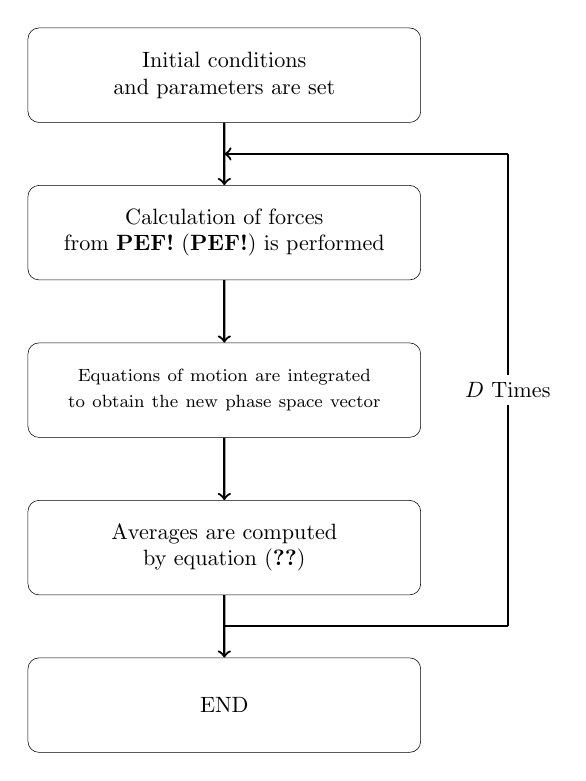
\begin{tikzpicture}[scale=0.8, transform shape]
	\node[rectangle,draw,rounded corners,very thin,minimum width=6cm,minimum height=1.5cm,text width=6cm,align=center] (A) at (0,10) {Initial conditions \\ and parameters are set};
	\node[rectangle,draw,rounded corners,very thin,minimum width=6cm,minimum height=1.5cm,text width=6cm,align=center] (B)  at (0,7.5) {Calculation of forces \\ from \ac{PEF} is performed};
	\node[rectangle,draw,rounded corners,very thin,minimum width=6cm,minimum height=1.5cm,text width=6cm,align=center] (C)  at (0,5) {\footnotesize Equations of motion are integrated to obtain the new phase space vector};
	\node[rectangle,draw,rounded corners,very thin,minimum width=6cm,minimum height=1.5cm,text width=6cm,align=center] (D)  at (0,2.5) {Averages are computed \\ by equation~(\ref{eq:MDTimeAve})};
	\node[rectangle,draw,rounded corners,very thin,minimum width=6cm,minimum height=1.5cm,text width=6cm,align=center] (E)  at (0,0) {END};
	\draw[thick,->] (A) -- (B);
	\draw[thick,->] (B) -- (C);
	\draw[thick,->] (C) -- (D);
	\draw[thick,->] (D) -- (E);
	\draw[thick,-] (0,1.25) -- (4.5,1.25);
	\draw[thick,-] (4.5,1.25) -- (4.5, 8.75) node[pos=0.5, fill=white] {$D$ Times};
	\draw[thick,->] (4.5, 8.75) -- (0, 8.75);
\end{tikzpicture}
\caption{Schematic representation of an \acs{MD} simulation.}
\label{fig:MDscheme}
\end{figure}

\subsection{Initial configuration}
Before an \ac{MD} simulation can be performed it is necessary to select an \textit{initial configuration}. Its 
choice can be nontrivial and it depends on the complexity of the system. Then, careful attention must be paid in 
setting up the initial configuration.

Setting up an initial configuration means to prepare an $N$--particle system and assign all particle positions 
and velocities, i.e. all the $6N$ coordinates of the initial phase space vector $\vec x(0)$. A common choice to 
assign the initial velocities is to extract they randomly from the Maxwell--Boltzmann distribution function at a 
specific system's temperature
\begin{equation*}
	f(v_i) = \sqrt{\frac{m_i}{2\pi k_B T}}e^{-\left ( \frac{m_iv_i^2}{2k_B T}\right )}
\end{equation*}
Moreover, the random assignment algorithm has to rescale all the velocities in such a way that the total system's 
momentum $\vec P = \sum_{k=1}^N m_k\vec v_k$ is zero, this is equivalent to a \ac{COM} motion removal. This is 
done because, in general, the total force acting on the system $\vec F = \sum_{k=1}^N \vec F_i$ is zero, then the 
\ac{COM} motion is constant and to avoid a constant drift of the system in space this can be removed. Of course 
this is a constraint on the system and it must be taken into account because it reduces the system \ac{DOF} by 
three.

\subsection{Periodic boundary conditions}
In an \ac{MD} simulation the sample system is inserted into a \textit{simulation box} whose shape can be 
differently chosen to better reproduce the symmetry of the simulated system. That box gives us the trivial 
possibility to introduce a well defined reference system of coordinates. Obviously we must not forget to 
correctly treat the \textit{boundary conditions}. In order to avoid surface effects and to consider only an 
infinite bulk system, \ac{PBC} are imposed to the simulation box. This gives us also the possibility to simulate 
system's bulk proprieties without considering a too large number of particles.
\begin{SCfigure}
	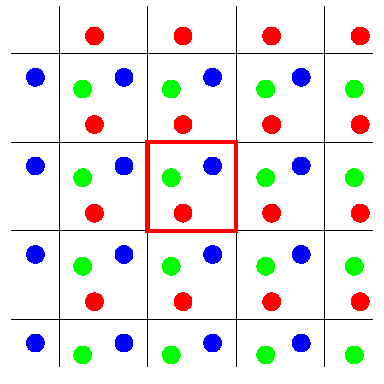
\includegraphics[width=0.5\textwidth]{./img/PBCScheme/PBCScheme}
	\caption{Schematic view of a two--dimensional box with \acs{PBC} imposed. The central, red contoured, box is the simulation box and it is replicated along each side.}
	\label{fig:pbc}
\end{SCfigure}
To give a better idea, in figure~(\ref{fig:pbc}) an example of a two--dimensional box with \ac{PBC} is shown. The 
central red contoured box is the simulation box. The idea is to replicate that box in space along each side so 
that there are no surface particles nor walls in the central box. When a particle moves in the central box, all 
its images virtually move the same way in the copies of the box so that if a particle leaves the virtual boundary 
of the central box, then, its nearest image enters the box and the number density of particles in the simulation 
box is conserved. This virtual movement of image particles is achieved adjusting the positions of the simulation 
box particles which have left the main box. For example, if one use a cubic box and a particle crosses its 
boundary in one direction, say the $x$ direction, then its coordinate is corrected by subtracting (if it leaves 
the box in the positive direction) or adding the box side length parallel to $x$ direction. Only box geometries 
compatible with translational symmetry can be used. For example, nether a spherical nor a icosahedral box could 
do the job. However when it is possible one have to use the most appropriate shape to better describe the 
symmetry of the system, otherwise a closest approximation, compatible with \ac{PBC}, must be used.

Even if \ac{PBC} are used in a wide range of applications, it must be taken into account that imposing 
periodicity to a system may affect its properties. A clear limitation of the periodic cell is that it is not 
possible to achieve fluctuations that have a wavelength greater then the cell length. This cause, obviously, the 
impossibility to sample those vibrating modes. Another problem arises with the range of the inter--particles 
interactions: one have to choose carefully the size of the simulation box, or the number of particles if an $NPT$ 
ensemble is used, to ensure that the smallest simulation box length is greater then the interaction range. This 
can be made easily for example with the Van der Waals interaction. On the contrary it is a difficult and time 
consuming task to do the same with the electrostatic interactions that are treated with a more sophisticated 
methods, as better explained in section~\ref{sec:longRangeInt}.

\subsection{Numerical integrators}
As we have seen above we need to solve numerically the equations of motion. Since the \ac{PEF} is a continuous 
function of the phase space vector at a time $t$, the simplest way is to use the so called \textit{finite 
difference} method. The basic idea is to expand the Newton's law in a Taylor series as follow
\begin{equation}
	\vec r_i(t + \delta t) = \vec r_i(t) + \vec v_i(t)\ \delta t + \frac{1}{2m_i}\vec f_i(t)\ (\delta t)^2\ +\ o((\delta t)^3)
	\label{eq:newtonTaylor}
\end{equation}
where we used the identities $\vec v_i(t) = \dot{\vec r}_i(t)$ and $m_i\ddot{\vec r}_i(t) = \vec f_i(t)$.

From this point, different algorithms have been developed. In the following we will describe in detail the most 
important, the \textit{Verlet algorithm}, and its implementation the \textit{leap--frog algorithm}, which is the 
default used in our \ac{MD} tools for this thesis work.

\subsubsection{Verlet algorithm}
The Verlet algorithm requires the positions and the forces at a time $t$ and the positions at a time $t-\delta t$ 
to calculate the positions at a time $t+\delta t$. Starting from equation~\eqref{eq:newtonTaylor} we can write
\begin{align}
	\vec r_i(t+\delta t) &\simeq \vec r_i(t) + \vec v_i(t)\delta t + \frac{1}{2m_i}\vec f_i(t)\ (\delta t)^2
	\label{eq:verlet1} \\
	\vec r_i(t-\delta t) &\simeq \vec r_i(t) - \vec v_i(t)\delta t + \frac{1}{2m_i}\vec f_i(t)\ (\delta t)^2
	\label{eq:verlet2}
\end{align}
from their sum we obtain the new positions at a time $t+\delta t$
\begin{equation}
	\vec r_i(t+\delta t) \simeq 2 \vec r_i(t) - \vec r_i (t - \delta t) + \frac{1}{m_i}\vec f_i(t)\ (\delta t)^2
	\label{eq:verletPosition}
\end{equation}
The velocities do not appear in the equation above and can be obtained taking the difference of 
equation~\eqref{eq:verlet1} and~\eqref{eq:verlet2}
\begin{equation*}
	\vec v_i(t) \simeq \frac{\vec r_i(t+\delta t) - \vec r_i(t-\delta t)}{2\delta t}
\end{equation*}

Since positions in equation~\eqref{eq:verletPosition} are computed as differences this is a fourth order 
algorithm and the precision is up to $o(\delta t)^4$, but they also contain a small term of order 
$o(\delta t)^2$, ($\vec f_i(t)/(2m_i)$) which is summed to a difference of larger terms 
($2 \vec r_i(t) - \vec r_i (t - \delta t)$). This may cause a loss of precision due to computer numerical representation.

The main disadvantage is that velocities at a time $t$ are an output of the calculation and not a part of the 
algorithm itself. Moreover it is not self--starting because the algorithm required the positions at a time 
$t-\delta t$. So at $t=0$ we need a trick to obtain the previous inexistent positions. The trick is to use 
equation~\eqref{eq:verlet2} truncated at the first order: $\vec r_i(-\delta t) \simeq \vec r(0) - \vec v_i(0)\delta t$.

\subsubsection{Leap--Frog algorithm}
The leap--frog algorithm is a variant of the Verlet one and it is commonly implemented in many \ac{MD} tools, as 
it is in our case. It computes the positions at a time $t$ and the velocities at a time 
$t+\nicefrac{1}{2}\delta t$ from the forces at a time $t$ and the velocities at a time 
$t-\nicefrac{1}{2}\delta t$. The main advantage with respect to the Verlet algorithm, is that it is 
self--starting because it does not require the positions at a time $t-\delta t$.

First it calculates the velocities at a time $t+\nicefrac{1}{2}\delta t$ as follow
\begin{equation*}
	\vec v_i(t + \nicefrac{1}{2}\delta t) \simeq \vec v_i(t - \nicefrac{1}{2}\delta t) + \vec a_i(t)\delta t
\end{equation*}
then the positions at a time $t+\delta t$ are computed
\begin{equation*}
	\vec r_i(t + \delta t) \simeq \vec r_i(t) + \vec v_i(t + \nicefrac{1}{2}\delta t)\delta t
\end{equation*}
The velocities at a time $t$ can be calculated by
\begin{equation}
	\vec v_i(t) \simeq \frac{\vec v_i(t + \nicefrac{1}{2}\delta t) + \vec v_i(t - \nicefrac{1}{2}\delta t)}{2}
	\label{eq:lfVelocitiesSync}
\end{equation}

Another advantage is that the velocities are part of the algorithm itself and moreover it does not require the 
calculation of the difference between two large numbers, with a gain of precision. The obvious disadvantage is 
that the positions and velocities are not synchronized so the equation~\eqref{eq:lfVelocitiesSync} is necessary 
to calculate the velocities at a time $t$. The need to have velocities at the same time of positions, as for the 
Verlet algorithm, derives from the calculation of the kinetic energy contribution to the total energy: it must be 
computed with positions and velocities at the same time.
%Discorso energia cinetica nello stesso tempo delle posizioni

\subsection{Neighbor list}
\label{sec:neighbor}
In order to solve the classical equations of motion, it is necessary to know the forces, and so the \ac{PEF}, 
acting on the system's particles. As we shall see in detail in the next section, this is one of the most time 
consuming part of an \ac{MD} simulation. To know the forces acting on one particle, in principle, it is necessary 
to calculate the contribution from all particles in the simulation box and all other periodic images. The most 
popular way to speed up the simulation is to use a truncation of the interaction potentials within a cutoff. The 
general idea is to compute the energy contribution of particle $i$ considering the interaction only with 
particles $j$ that are closer to a certain cutoff distance $r_c$, thus such that 
$\|\vec r_i - \vec r_j\| \le r_c$. This is summarized in the following expressions
\begin{equation*}
	U_i(\vec r) = \sum_{j\ne i}^N U^*_{ij}(\vec r), \qquad U^*_{ij}(\vec r) = \left \{
	\begin{aligned}
		& U_{ij}(\vec r)& \qquad  &\| \vec r_i - \vec r_j \| \le r_c \\
		& 0			    & \qquad  &\text{otherwise}
	\end{aligned}
	\right .
\end{equation*}
where $U_{ij}(\vec r)$ is the interaction potential between particles $i$ and $j$.

By itself, the use of a truncation of the potential may not dramatically reduce the time spent in computing the 
inter--particle interactions. This is because, in order to decide for what particles we have to compute the 
interactions, we have to compute the distances between every pair of particles in the system. A marked increase 
of performance is achieved by the use of a \textit{neighbor pair--list}. The simplest way is to consider, for 
each particle, a list of its neighbor particles that lie within a sphere of radius $r_c$ surrounding the selected 
particle. Then, for each particle, the interactions are computed between the selected particle and those that are 
in its pair--list. There is a gain in performance if the pair--list is updated at least every $M>1$ \ac{MD} 
steps. This is possible taking into account that, typically, in \ac{MD} simulations of liquids system at ambient 
temperature and pressure, a particle neighbors do not change significantly for $M < 20$ time steps.

Anyway particles move during the non--updating time so that some of them may cross the pair--list causing an 
over-- or under--estimation of the inter--particle energy contribution. To partially solve this problem, as 
suggested by Verlet \cite{VerletList}, one can consider a \textit{buffered} pair--list or a \textit{Verlet 
cut--off scheme} in which the pair--list is constructed considering those particles that are close to the 
selected one by a distance of $r_l > r_c$, called \textit{list radius}. That pair--list is updated every some 
time steps, but every time steps the pairwise contribution is computed only between those particles in the 
pair--list for which the distance is less then $r_c$. Thus, at the cost of slightly decrease the performance 
compared to the un--buffered pair--list, almost none of the interacting particles within the cutoff is neglected. 
Nevertheless, since a too big list radius and a too small list update frequency leads to a loss of performance, 
particle--pairs could still move enough during the non--updating time and have a chance to cross the boundary of 
the buffered pair--list $r_l$. This chance leads to a small energy drift proportional to the system temperature. 
In simulations with a constant temperature coupling, i.e. in a canonical or isothermal--isobaric ensemble, the 
extra radius of the buffered pair--list can be dynamically determined, during the simulation, by fixing an upper 
limit to the energy drift. That tolerance is often called \textit{Verlet buffer tolerance}. In 
figure~(\ref{fig:pairlist}) a schematic representation of the buffered pair--list construction is shown.
\begin{SCfigure}
	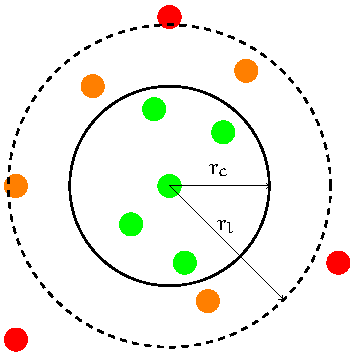
\includegraphics[width=0.42\textwidth]{./img/pairList/pairList}
	\caption{Schematic representation of the buffered pair--list construction respect to the central particle.
	Green particles are in the pair--list below the cutoff radius $r_c$, therefore included in the calculation of the interactions. Orange particles are in the pair--list for which at every step is checked if their distances became smaller then $r_c$. Red particles are not in the pair--list and they are completely neglected until the next list update.}
	\label{fig:pairlist}
\end{SCfigure}

A better performance can be achieved adding a dynamic update algorithm of the pair--list refresh rate during the 
simulation. A nice way is to consider the maximum distance traveled by a particle in the pair--list: if this 
distance is greater than $r_b = r_l - r_c$ then the pair--list is certainly updated. Thus one can fix the refresh 
rate to a higher value increasing the performance.

\subsection{Thermostat algorithms} %Molecular Modelling, 382
A thermostat is an external tool that allows to maintain a system at a constant temperature. Several algorithms 
are available. Some are based acting on particle velocities (Anderson, Berendsen, Bussi) other introduce some 
more \ac{DOF} in the system that take into account a real temperature bath coupling (Nosé--Hoover). We will 
describe in more detail the one used in this thesis work.

As suggested by Bussi \etal\, \cite{Bussi}, a common practice to implement a thermostat acting on particle 
velocities is related to a \textit{velocity rescale} algorithm in which the velocities of all particles are 
scaled by some factor. The simplest way is to consider the total kinetic energy $K$ of the system as in 
equation~\eqref{eq:kinetic} and the average kinetic energy $\ave{K}$ obtained from equation~\eqref{eq:kineticT} 
with the substitution $3N\rightarrow N_f$
\begin{equation*}
	\ave{K} = \frac{1}{2}N_f k_B T
\end{equation*}
where $N_f$ is the \textit{total} \ac{DOF} of the system and $T$ is the target temperature. Thus the scaling 
factor is defined by
\begin{equation*}
	\alpha_{T} \equiv \sqrt{\frac{\ave{K}}{K}}
\end{equation*}

The scaling operation is usually performed at a fixed rate during the simulation, or when the kinetic energy 
exceeds the limits of an interval centered around the target value. However the sampled ensemble is not 
explicitly known but, since in the thermodynamic limit the average properties do not depend on the ensemble 
chosen, even this very simple algorithm, often called \textit{weak coupling thermostat}, can be used to produce 
useful results. Despite this, for small systems or when the observables of interest are dependent on the 
fluctuations rather than on the averages or when other methods assume a canonical sampling, this method cannot be 
safely used.

In order to obtain the correct canonical sampling Bussi \etal\, \cite{Bussi} modify the way to calculate 
$\alpha_T$ so as to enforce a canonical distribution for the kinetic energy. The new scaling factor is obtained 
from
\begin{equation*}
	\alpha_{T} \equiv \sqrt{\frac{K_T}{K}}
\end{equation*}
where $K_T$ is extracted with a stochastic procedure from the equilibrium canonical distribution of the kinetic 
energy, given by
\begin{equation*}
	P(K_T)dK_T \propto K_T^{N_f/2-1}\ e^{-\beta K_T}\ dK_T
\end{equation*}
where $P(K_T)dK_T$ is probability that the system has a kinetic energy between $K_T$ and $K_T + dK_T$.

Since velocities are scaled only after some \ac{MD} steps this can cause a discontinuity in the particles 
velocities just before and after the scaling step. To avoid this problem, the authors suggest that the choice of 
$K_T$ can be based on the previous value of $K$ so as to obtain a smoother evolution. The procedure proposed by 
Bussi \etal\, consists in the following steps
\begin{itemize}
	\item Evolve the system for a single time step solving the equations of motion, so as to be in an $NVE$ ensemble;
	\item Calculate the total kinetic energy and evolve it for a single time step using an auxiliary continuous stochastic dynamics;
	\item Rescale the velocities by $\alpha_T$ so as to enforce this new value of the kinetic energy.
\end{itemize}

The authors have shown that an auxiliary dynamics for the kinetic energy of the form
\begin{equation*}
	dK = \frac{\ave{K} - K}{\tau_T}\ dt + 2 \sqrt{\frac{K\ave{K}}{N_f\tau_T}}\ dW
\end{equation*}
can do the job. Where $dW$ is a Wiener stochastic noise and $\tau_T$ is an arbitrary parameter which is related 
to the response time of the thermostat. In fact it reduces to the simple week coupling rescale if 
$\tau_T\rightarrow 0$ and to the Hamiltonian dynamics (as an $NVE$ ensemble) if $\tau_T\rightarrow +\infty$. 
Until the system is at non--equilibrium the first deterministic part is dominant an drives the system to 
equilibrium with a characteristic time $\tau_T$. Then the stochastic contribution samples the canonical 
distribution.
 

\subsection{Barostat algorithms} %Molecular Modelling, 382
As the thermostat maintains the system at a constant temperature $T$, a barostat is needed to maintain the system 
at a constant pressure $p$. To do this the system is coupled to a sort of piston so that changing the volume of 
the simulation box will adjust the pressure.

\subsubsection{Berendsen algorithm}
A common way, as proposed by Berendsen, is to scale both volume and particle coordinates. The rate of change of 
the pressure is given by
\begin{equation*}
	\frac{dp}{dt} = \frac{p_0 - p}{\tau_p}
\end{equation*}
where $p_0$ is the target pressure, $p$ is the instantaneous system pressure given by 
equation~\eqref{eq:pressure} and $\tau_p$ is a coupling constant related to the response time of the barostat. 
Thus if we consider a time step $\delta t$ then the volume scaling factor $\lambda$ is given by
\begin{equation*}
	\lambda = 1- k_T (p_0 - p) \frac{\delta t}{\tau_p}
\end{equation*}
where $k_t$ is the isothermal compressibility defined as
\begin{equation*}
	k_T = -\frac{1}{V}\left ( \frac{\partial V}{\partial p}\right )_{T}
\end{equation*}
while the factor $\nicefrac{\delta t}{\tau_p}$ gives a scaling factor for the isothermal compressibility that 
allow us to take into account the finite response time of the barostat. If $\tau_p \rightarrow 0$ the system has 
an infinity isothermal compressibility so it is necessary a really small change in volume to achieve the correct 
pressure; on the contrary if $\tau_p \rightarrow +\infty$ the system reduces to the Hamiltonian 
dynamics\footnote{If the system is coupled to a thermostat, then the canonical ensemble is sampled.}. The 
particle coordinates is scaled by the factor $\lambda^{\nicefrac{1}{3}}$.  

In the case of anisotropic system the pressure matrix $\mathbold{P}$ and the volume matrix $\mathbold{H}$ have to 
be considered and the Berendsen algorithm can be generalized such that even $\lambda$ becomes a $3\times 3$ 
matrix. However the main problem, as for the weak coupling thermostat, is that the sampled ensemble is not known. 
Thus a new approach, in order to correct sample the isobaric ensemble, has been derived by Parrinello and Rahman.

\subsubsection{Parrinello--Rahman algorithm}
The Parrinello--Rahman barostat \cite{ParrinelloBarostat1}\cite{ParrinelloBarostat2} is based on genuinely treat 
the coupling of the system to an external piston of ``mass'' $M_h$ through a Lagrangian method in which the 
volume becomes a Lagrangian variable of the system and its time evolution can be computed solving the 
Euler--Lagrange equations. Both the size and the shape of the simulation box are allowed to fluctuate. So it is 
perfectly compatible with anisotropic system. The shape and size of the simulation box are described by the 
volume matrix $ \mathbold{H}$ in equation~\eqref{eq:volumeMatrix} such that $V = |\det\mathbold{H}|$. 
$\mathbold{H}$ is the Lagrangian coordinate of the external piston. If the external pressure $p_0$ is applied to 
the piston then its potential energy is given by
\begin{equation*}
	U_p = p_0 |\det  \mathbold{H}|
\end{equation*}
instead, if $ \mathbold{H}$ varies in time then a ``kinetic energy'' is associated to the piston as follow
\begin{equation*}
	K_p = \frac{1}{2}M_h \text{Tr}(\leftidx{^t}{\dot{ \mathbold{H}}}{} \dot{ \mathbold{H}} )
\end{equation*}
where $\leftidx{^t}{(\cdot)}{}$ denote the transpose operation.

In order to write the Lagrangian of the system the particle coordinates must be expressed in terms of 
$\mathbold{H}$. This can be done defining the vector $\vec s_i$ so that $\vec r_i =  \mathbold{H} \vec s_i$. The 
square displacement can be obtained as $\vec r_i \cdot \vec r_i = \leftidx{^t}{ (\mathbold{H} \vec s_i)}{}  \mathbold{H} \vec s_i = \leftidx{^t}{\vec s_i}{} \leftidx{^t}{ \mathbold{H}}{}  \mathbold{H} \vec s_i$, often 
$\mathbold{G} = \leftidx{^t}{ \mathbold{H}}{} \mathbold{H}$. Parrinello \etal\, write the Lagrangian as follow
\begin{equation*}
	\mathcal{L} = \frac{1}{2}\sum_{i=1}^N m_i \dot{\vec s}_i \leftidx{^t}{\mathbold{G}}{} \dot{\vec s}_i - \sum_{i=1}^N \sum_{j=i+1}^N U_{ij}(\vec r) +  \frac{1}{2} M_h \text{Tr}(\leftidx{^t}{\mathbold{\dot H}}{} \mathbold{\dot H} ) -  p_0 |\det \mathbold{H}|
\end{equation*}
thus the equations of motion for $ \mathbold{H}$ and $\vec s_i$ can be computed solving the Euler--Lagrange 
equations. It can be shown that those equations of motion, derived in \cite{ParrinelloBarostat1} and 
\cite{ParrinelloBarostat2}, correct sample an isobaric ensemble. A practical way to show this is to consider the 
Hamiltonian of the system. Using equation~\eqref{eq:hamiltonian} the Hamiltonian is
\begin{equation*}
	\mathcal{H} = \frac{1}{2}\sum_{i=1}^N m_i \dot{\vec s}_i \leftidx{^t}{\mathbold{G}}{} \dot{\vec s}_i + \sum_{i=1}^N \sum_{j=i+1}^N U_{ij}(\vec r) +  \frac{1}{2} M_h \text{Tr}( \leftidx{^t}{\mathbold{\dot H}}{} \mathbold{\dot H} ) + p_0 |\det\mathbold{H}|
\end{equation*}
if the system is in equilibrium at temperature $T$, using the equipartition theorem, the kinetic term of the 
system particles contributes to the energy by $3Nk_BT/2$ while the kinetic term of the piston by $9k_BT/2$. Thus 
since $3N \gg 9$ the Hamiltonian can be approximated by
\begin{equation*}
	\mathcal{H} \simeq \ave{K} + U + p_0 V = H
\end{equation*}
that is the enthalpy. Since the Hamiltonian is a constant of motion the correct isobaric ensemble is sampled. If 
the system is also coupled to a thermostat, the $-TS$ term must be added, so the constant of motion become the 
Gibbs free energy $G = H - TS$ and the isobaric--isotherm ensemble is correctly sampled.

In order to understand the meaning of the $M_h$ parameter (the piston ``mass'') we report the dynamic equation of $\mathbold H$
\begin{equation*}
	M_h \mathbold{\ddot H} = V (p - p_0) (\leftidx{^t}{\mathbold{H}}{})^{-1}
\end{equation*}
The Parrinello--Rahman barostat is like a second order system. When there is an imbalance between the 
instantaneous internal pressure $p$ (see equation~\eqref{eq:pressure}) and the target pressure $p_0$, the system 
recovers this imbalance in a characteristic time governed by the parameter $M_h$. Since at equilibrium the 
properties of a system are independent of the masses of its constituent parts, $M_h$ can be arbitrarily chosen if 
one is interested only in static averages, otherwise a more appropriate choice must be made to obtain accurate 
dynamical properties. In this case, the authors suggest a choice of $M_h$ such that the relaxation time is of the 
order of $L/c$ where $L$ is simulation box size and $c$ is the sound velocity. 

Interesting is the fact that this algorithm can be generalized to an anisotropic pressure coupling making use of 
the theory of elasticity. Differently from the Berendsen algorithm, Parrinello--Rahman method is much slower in 
changing the volume until the equilibrium value is reached and it is less stable: if the system is not well 
equilibrated can lead to a large volume fluctuation with can compromise the simulation success. On the other hand 
the Parrinello--Rahman samples correctly the isobaric ensemble. A common strategy is to use the Berendsen 
barostat to reach equilibrium then switch to the Parrinello--Rahman algorithm to correctly sample the phase space 
associated to the isobaric ensemble.

\section{Empirical Force--Field model}
\label{sec:EmpiricalFF}
As we have seen in the previous section \ac{MD} provides a variety of tools for solving the time evolution of a 
$N$--particle system. Due to the possibility to capture different length and time scales \ac{MD} simulations can 
be used in a variety of systems, such as set of atoms, molecules or more complex system such as protein and 
macromolecules systems. In each of these systems, depending on the \textit{interaction model} and its 
\textit{parametrization}, we will be able to describe crucial molecular--level processes, such as hydrogen bond 
formation in organic molecules, which happen on the picoseconds time scale; or study slow processes such as the 
diffusion of massive colloidal particles, taking place on time scales of milliseconds if not seconds.

Considering soft or condensed mater, the most relevant for this thesis work, the main processes of interest 
ranging from protein folding to glass transitions, from surface diffusion to ligand--receptor binding take place 
on longer time scales (several ns) and involve a larger number of atoms ($N \gg 10^4$). In this case a crucial 
role is played by the \textit{Born--Oppenheimer approximation}. It says that we can separate the motion of the 
electrons by the motion of the atomic nuclei. This is done in order to integrate out the high frequency 
electrons' motions and to remove some \ac{DOF} due to the necessity to increase the time step and speed up the 
simulation. If, for some particular system, we want to know precisely the dynamics of the electrons we have to 
introduce quantum mechanical methods that are, even for a small number of particles ($N\sim 10^2$), very 
computationally time consuming. In the following, when we speak about atoms or chemical moieties we refer to it 
as for nuclei coordinates only without considering electrons at all.

Nevertheless atom or molecule interactions, such as bond formation, are mediated by the electron interactions. 
Thus, to describe the dynamics of such a system with a classical \ac{MD} tools and the Born--Oppenheimer 
approximation, it is necessary to develop an \textit{empirical model of the inter--atom interactions} that mimics 
the interactions behavior. Since forces are derived from the \ac{PEF}, a typical choice, when it is possible, for 
example with organic systems, is to model the inter--particle interactions by a set of pairwise addictive 
potentials that avoid any many--body calculations. Nevertheless for some systems this is impracticable, for 
example, for metal cores we need to consider the many--body calculations or an effective many--body potential 
that take into account the behavior of all metal atoms in the core. A typical solution is to use the many--body 
potential developed by Gupta (see \cite{Leach} for more details about metals treatment at \ac{MD} level). The set 
of functional forms of the inter--particle interaction potentials and its parameterization are collected into the 
so called empirical \acf{FF}. The meaning of \textit{empirical} is that most of the functional forms of the 
interactions has no ``first principle'' justification: they are chosen as a compromise between accuracy and 
computational efficiency. 
%Further it is necessary to stress out that a \ac{FF} is a well defined single entity containing the simulation parameters, the functional models of the interactions and also its parameterizations (and the way to obtain it). All the parameters of a \ac{FF} are in harmony to each other thus changing some parameters without retesting whole \ac{FF} is not allowed because, maybe, one can destroy the whole \ac{FF}.

For biomolecular applications two main classes of \acp{FF} exist: the \textit{atomistic} \acp{FF} in which basic 
particles are atoms, and the \textit{\ac{CG}} \acp{FF} in which the basic particles represent atom groups or 
small chemical moieties. In this case, even the way to realize the grouping, called \textit{mapping}, is part of 
the \ac{FF} itself. Different \ac{CG} \acp{FF} can use different mapping methods even with the same functional forms. 

In the following we will add some other information about \acp{FF} and describe the principal functional forms 
for modeling the inter--particle interactions and how to treat them in an \ac{MD} simulation. While in the next 
section we will focus on the main \ac{CG} \ac{FF} used in this thesis work: the \textacr{MARTINI} \ac{FF} 
developed by Marrink \etal\, \cite{Martini}.

\paragraph{\textbf{\textacr{parameterization}}} In general the functional forms for potential interactions are 
common to all particles in the system. The \ac{FF} is completed by a set of empirical parameters that 
characterize the interaction between different types of particles, whether they are atoms or whole chemical 
groups. Interaction parameters are empirical in the sense that they are assigned to reproduce a small set of 
target properties on a small group of systems. These target properties can be derived from experimental 
measurements or from finer--level calculations or simulations. Nowadays, atomistic and \ac{CG} biomolecular 
\acp{FF} come as ``packages'' of parameters and functional forms appropriate for the description of a large 
variety of chemical compounds in the liquid and solid phases.

\paragraph{\textbf{\textacr{transferability}}} As described above the parameterization of a \ac{FF} involves a 
small set of test systems for which some set of target proprieties are reproduced. The main characteristic of a 
\ac{FF} is the \textit{transferability} that means the ability of the model to describe different situations that 
differ from those used at the parameterization stage. Of course one would expect to be able to make some 
predictions for a bigger variety of systems and for other proprieties not used in the parametrization stage. 
Common faults of organic \acp{FF} concern, for example, phase transitions of organic compounds and phase 
transition temperatures.

\subsection{Inter--particles interactions}
For biomolecular applications the inter--particle interaction potentials are divided into two main classes: the 
\textit{bonded interactions} involving particles within the same molecules and the \textit{non--bonded 
interactions} engaging all particles in the system and which usually represent the Van der Waals and the 
electrostatic interactions. In the following the most common and general functional form for the \ac{PEF} is 
descried. In general the \ac{PEF} can be always splitted in a bonded and non--bonded contributions:
\begin{equation*}
	U(\vec r) = U_{\text{b}}(\vec r) + U_\text{nb}(\vec r)
	\label{eq:FFPEF}
\end{equation*}

The bonded contribution is generally described by the following terms
\begin{equation}
	\begin{aligned}
	U_{\text{b}}(\vec r) = &\frac{1}{2}\sum_{\text{bonds}} \frac{1}{2}k_i^b(l_i - l_{i0})^2\ + \frac{1}{2}\sum_{\text{angles}} k_i^a (\theta_i - \theta_{i0})^2 +\\
		 	& +\frac{1}{2}\sum_{\text{torsions}} V_n(1+\cos (n\omega - \gamma))
	\end{aligned}
	\label{eq:bondPEF}
\end{equation} 
the first two terms are harmonic potentials which model respectively the energy contribution due to the deviation 
from reference bond length $l_{i0}$ and a bond angle $\theta_{i0}$. $k_{bi}$ and $k_{ia}$ are the bond and angle 
elastic constants. The bond contribution involve a set of two particles in the some molecule while the angle 
contribution a set of three particles in the same molecule. The last term in equation~\eqref{eq:bondPEF} concerns 
the energy contribution due to the bond torsional change. It involves four particles in the same molecule and 
mimic the energy barrier needed to rotate the bond angle along the bond axis. $\omega$ is the torsional angle, 
$\gamma$ is a phase factor, $V_n$ qualitatively describes the energy barrier for each $n$--th components and $n$ 
is defined as the number of minima for each components.

The non--bonded contribution is described by the following terms
\begin{equation}
	U_\text{nb}(\vec r) = \sum_{i=1}^N \sum_{j>i} \left ( {4\epsilon_{ij} \left ( \left ( \frac{\sigma_{ij}}{r_{ij}} \right )^{12} - \left ( \frac{\sigma_{ij}}{r_{ij}} \right )^6 \right )  + \frac{q_iq_j}{4\pi\varepsilon_0 r_{ij}}} \right )
	\label{eq:nonbonPEF}
\end{equation}
The first term is the energy contribution due to the Van der Waals interactions modeled as a Lennard--Jones 
$12-6$ potential, fully characterized by the constants $\sigma_{ij}$ and $\epsilon_{ij}$ proper for each 
particles pair. The last term is the electrostatic energy contribution described by the particle charge $q$. The 
non--bonded interactions involve obviously all particles in the system, but for particles belonging to same 
molecule they are computed only if they are separated by at least three bonds, i.e. if their interactions are not 
described by bonded terms. The various contributions described above are schematically represented in 
figure~(\ref{fig:FFInteraction}).
\begin{figure}[!ht]
	\centering
	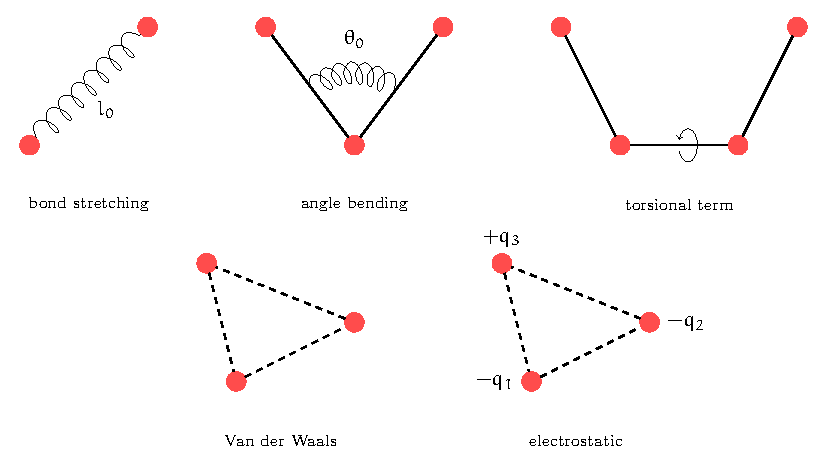
\includegraphics[width=0.8\textwidth]{./img/interPartInt/interPartInt}
	\caption{Schematic representation of the common inter--atom interactions for biomolecular applications: bond stretching, angle bending, torsional term, Van der Waals and electrostatic interactions.}
	\label{fig:FFInteraction}
\end{figure}

\subsection{Non--bonded interactions}
\label{sec:nonbonded}
The bonded interactions, as we can see in equation~\eqref{eq:bondPEF}, are at \textit{fixed range}, meaning that 
they depend, for example, on the equilibrium bond length that is fixed. Moreover, usually in standard \ac{MD} 
simulations the bond break is not taken into account. The same does not hold for the non--bonded interactions 
because they depend on the inter--particles distance $r_{ij}$ and they decay to zero as a power of $r_{ij}^{-d}$. 
Depending on the power order $d$ compared to the dimensionality $s$ of the system they are split into 
\textit{short range} if $d>s$ and \textit{long range} interactions if $1 \le d < s$. For example, as we shall see 
later, the Lennard--Jones $12-6$ potential decays to zero as $r^{-6}$ then it is a short range interaction, while 
the electrostatic is a long range interaction since it decays to zero as $r$.

\subsubsection{Cut--off, shift and switch methods}
As we have mentioned in section~\ref{sec:neighbor} the calculations of non--bonded interaction energy 
contributions is one of the most time consuming part of an \ac{MD} simulation. Even if we use a simple pairwise 
additive potential their calculation scale as $\sim N^2$. Thus, especially for short range interactions, various 
methods were developed in order to speed--up the simulation. The \textit{cut--off} method is the most used to 
treat the short range interactions and, in some cases, even the long range ones. Taking one particle into 
account, the general idea is to evaluate the non--bonded interactions with all other particles that are closer to 
the first for a distance $r_c$, called \textit{cut--off} radius, otherwise the interactions is set to $0$. This 
means that the new potential is of the form
\begin{equation*}
v^*(r) = \left \{
	\begin{aligned}
&v(r) & \quad & r \le r_c \\
&0    & \quad & r >   r_c
	\end{aligned} \right .
\end{equation*}

This generates a discontinuity in the potential and in its first derivatives, i.e. in the forces: this is bad for 
energy conservation. A trick for solving the discontinuity of the potential and to improve the energy 
conservation is to apply also a \textit{shift} of the potential value at $r_c$ so that $v^*(r_c) = 0$. Adding a 
constant will not affect the force calculations. The potential becomes
\begin{equation*}
v^*(r) = \left \{
	\begin{aligned}
&v(r) - v(r_c) & \quad & r \le r_c \\
&0    & \quad  & r >   r_c
	\end{aligned} \right .
\end{equation*}

Moreover, to solve the discontinuity of the forces, that can cause some instability, a simple possibility is to  
consider a linear term proportional to the first derivative of the potential, such as
\begin{equation*}
v^*(r) = \left \{
	\begin{aligned}
&v(r) - v(r_c) - \left . \frac{dv(r)}{dr}\right |_{r_c}\ (r - r_c) & \quad & r \le r_c \\
&0    & \quad  & r >   r_c
	\end{aligned} \right .
\end{equation*}
The shift methods can make the potential quite different from the original one. So this have to be properly taken 
into account in order to retrieve the correct thermodynamics proprieties.

Another powerful method to solve the discontinuity problem of the potential and forces is the \textit{switch} 
method. The general idea is to consider two cut--off radii  $r_{c1}$ and $r_{c2}$. If $r \le r_{c1}$ the original 
form is used; while if $r > r_{c2}$ the potential is set to zero. If $r_{c1} < r \le r_{c2}$ a \textit{switching 
function} is considered in order to \textit{smoothly} switch the potential to zero.

It is important to stress out that even the method used to treat the interactions, as the cut--off radii and 
eventually the switching function, are part of the simulation parameters that are, in turn, part of the \ac{FF}. 
So they are interdependent with the model parameterization, and should never be changed without retesting the 
target properties of the parameterization.

\subsection{Van der Waals interactions}
Van der Waals forces are a set of interactions that can be ascribed to quantum dynamic effects. In general they 
are described by a sum of a repulsive and an attracting term. The former effectually takes into account the Pauli 
exclusion principle between electron clouds; the latter is related to the dipole--dipole interactions (Keesom 
forces), dipole--induce dipole interactions (Debye forces), induced dipole--induced dipole interactions, London 
dispersion forces, hydrogen bonding and entropy effects, that involves both polar and non--polar atoms. 

The usual way to treat the Van der Waals interactions is to use a pairwise Lennard--Jones potential. The most 
common exponents for the attractive and repulsive contributions are $6$ and $12$, respectively. The former has 
physical meaning: calculating the repulsive part of the Van der Waals interaction for a simple system in a 
semi--classical approximation gives a potential energy contribution that vanishes as $r^{-6}$. While the latter 
is only for computational reason: giving the $r^{-6}$ term it is efficiency to calculate $r^{-12}$ as the square 
of $r^{-6}$. Thus it is just a common choice and other exponents can do the job, depending on the system in 
study. The general form for a $12-6$ Lennard--Jones potential is the following
\begin{equation}
	v(r) = 4\epsilon\left ( \left ( \frac{\sigma}{r}\right )^{12}  - \left ( \frac{\sigma}{r} \right )^6 \right ) = \frac{C_{12}}{r^{12}} - \frac{C_{6}}{r^{6}}
	\label{eq:lj126}
\end{equation}
where $C_{12} = 4\epsilon\sigma^{12}$, $C_{6} = 4\epsilon\sigma^{6}$ and $r$ is the pairwise particles distance. 
$\epsilon$ is related to the absolute value of minimum while $\sigma$ is related to the position of the minimum 
of the potential: $r_{\text{min}} = 2^{\nicefrac{1}{6}}\sigma$, often referred to by Van der Waals radius. These 
constants are proper for each particle pair. The attractive contribution is due to the negative part proportional 
to $r^{-6}$ while the repulsive one is due to the positive part proportional to $r^{-12}$. In 
figure~(\ref{fig:LG12511}) a plot of the function~\eqref{eq:lj126} with $\epsilon = \sigma = 1$ is shown.
\begin{figure}[!ht]
\centering
	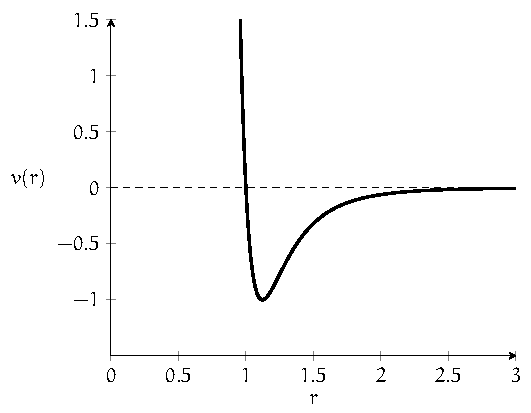
\includegraphics[width=0.6\textwidth]{./img/LJ126/LJ126}
	\caption{Plot of a Lennard--Jones interaction potential with $\epsilon = \sigma = 1$.}
	\label{fig:LG12511}
\end{figure}

The simplest and computationally most efficient way to treat a Lennard--Jones function, and in general all the 
short range interactions, is to use the cut--off method together with the shift or switch methods in order to 
obtain a continuous potential and/or a continuous forces. As we can see from figure~(\ref{fig:LG12511}) the 
Lennard--Jones potential vanishes rapidly with distance: at $r \sim 2\sigma$ its value is less then $1\%$ of the 
value in $r \sim \sigma$. A good choice for the cut--off is then of the order of $r_c \sim 2\sigma \div 3\sigma$.

\subsection{Electrostatic interactions}
\label{sec:longRangeInt}
Despite the long range characteristic of the electrostatic interaction, for computational efficient reason, most 
of the \acp{FF} for biomolecular applications treat them in the same way as a short range interaction by a 
cut--off method\footnote{In general, for computational reason, a common choice is to consider the same cut--off 
for Van der Waals and electrostatic interactions.}. Of course this is an approximation and can lead to serious 
issues in those proprieties or systems that strongly depend on the electrostatic interactions. As an example we 
report some situations in which the use of the short--range electrostatics can lead to artifacts: they are 
related to the development of a good polar solvent model (a good treatment of the electrostatic proprieties of 
water is really important for biological applications), as well as to the study of the interactions of charged 
particles with polar solvents, transport processes of charged moieties, calculations of the electrostatic 
potential inside macromolecules and so on. The calculation of the electrostatic energy contribution requires to 
take into account \textit{all particles} in a system, even all the periodic images due to the \ac{PBC}. This 
leads to a loss of computational efficiency.

If we consider only the simulation box the electrostatic energy contribution is
\begin{equation}
	U = \frac{1}{2}\sum_{i=1}^N\sum_{j\ne i}^N\frac{1}{4\pi\varepsilon_0}\frac{q_iq_j}{r_{ij}}
	\label{eq:electrostatic}
\end{equation}
where $q_i$ and $q_j$ are the charge of particles $i$ and $j$ and $r_{ij}$ is the distance between $i$ and $j$. 
But we need also all image boxes. Supposing, for simplicity, that the box is a cube of size $L$, then we can 
define a tern of integer numbers $(n_x,\ n_y,\ n_z)$, $n_i=0,1,2,\cdots$ so that the position of all other image 
boxes, with respect to the central simulation box, is $\vec n = L (n_x,\ n_y,\ n_z)$. Then the energy 
contribution becomes
\begin{equation}
	U = \frac{1}{2}\ \sideset{}{'}\sum_{n_x,n_y,n_z}^{+\infty}\ \sum_{i=1}^N\sum_{j=1}^N\frac{1}{4\pi\varepsilon_0}\frac{q_iq_j}{\|\vec r_i - \vec r_j + \vec n \|}
	\label{eq:electrostaticImage}
\end{equation}
where the prime indicates that for $\vec n = 0$, i.e. the energy contribution of the simulation box, we need to 
exclude the self interaction term: in the inner sum it must be $j \ne i$.

As described above, a cut--off method is a good easy way to solve equation~\eqref{eq:electrostatic} and sometimes 
it produces sufficiently good results. However, the increasing of computer power can lead to develop more 
rigorous methods to solve equation~\eqref{eq:electrostaticImage}, even for very large systems. The main problem 
is that the summation in equation~\eqref{eq:electrostaticImage} is \textit{conditionally convergent}\footnote{A 
conditionally convergent series contains both positive and negative terms such that the positive or negative term 
alone form both a divergent series. The sum of a conditionally convergent series depends on the order in which 
the positive and negative terms are considered.} and converges extremely slowly so that it would need so many 
terms to converge that its computational cost would be too high, especially for large systems (of the order of 
$N > 10^4$). The most important methods developed to solve this problem are based on the \ac{ESM}. We shall 
describe those used in this thesis work: the \ac{ESM} itself and the \ac{PME} method. For a more complete 
discussion about the advanced methods developed to treat the electrostatic interactions for biological 
applications the reader is addressed to the review by Cisneros \etal\, \cite{Cisneros}.

\subsubsection{Ewald summation method} %Molecular Modelling, 334
The \acf{ESM} is the first method introduced by Ewald for a correct treatment of the electrostatic energy 
contribution in an ionic crystal. The basic idea is to split the summation in equation~ 
\eqref{eq:electrostaticImage} in two series both rapidly convergent. The method is based on the following identity
\begin{equation}
	\frac{1}{r} = \frac{f(r)}{r} + \frac{1 - f(r)}{r}
	\label{eq:ewaldTrick}
\end{equation}
the trick is to choose a function $f(r)$ that will deal with the rapid variation of the $1/r$ term for small $r$ 
and the slow decay at long $r$; in that case the two series can rapidly converge.
\begin{figure}[!ht]
	\centering
	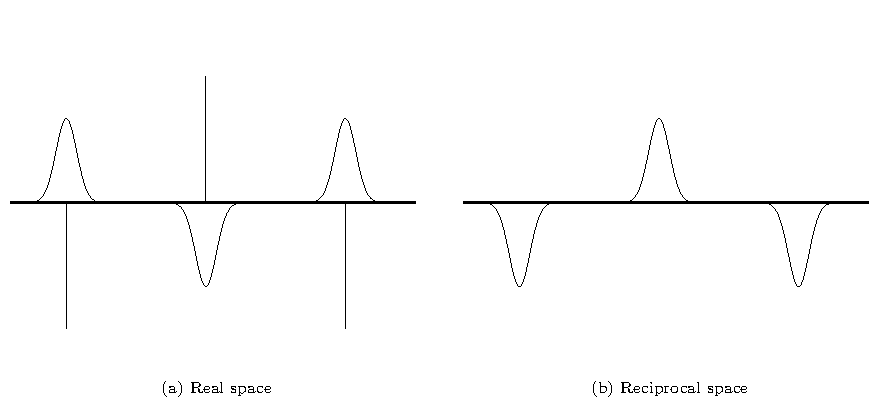
\includegraphics[width=0.8\textwidth]{./img/EwaldSum/EwaldSum}
	\caption{Schematic illustration of the \acs{ESM} charge distribution: in (a) point charges (represented by vertical lines) and the neutralizing Gaussian charge distribution; in (b) the counteracting Gaussian distribution.}
	\label{fig:ewald}
\end{figure}

The \ac{ESM} for electrostatic interactions works, as illustrated in figure~(\ref{fig:ewald}), considering each 
point--like charge in the system surrounded by a neutralizing charge distribution of equal magnitude but opposite 
sign that decays rapidly to zero. Simplifying the notation for a one dimensional system, the simplest functional 
form is a Gaussian distribution centered in the position $r_i$ of the point--like charge $q_i$, of the form
\begin{equation}
	\rho_i(r) = \frac{q_i\alpha^3}{\pi^{3/2}}e^{-\alpha^2 (r - r_i)^2}
\end{equation}
that obeys the relation
\begin{equation*}
	\frac{q_i\alpha^3}{\pi^{3/2}}\int_{r_i-\epsilon}^{r_i+\epsilon}e^{-\alpha^2 (r - r_i)^2}\ dr \simeq q_i
\end{equation*}
where $(r_i-\epsilon; r_i+\epsilon)$ is a small interval around $r_i$. The energy contribution due to this set 
up, the point--like charge \textit{and} the gaussian charge distribution, is given by
\begin{equation}
	U_r = \frac{1}{2}\sum_{i=1}^N\sum_{j=1}^N\ \sideset{}{'}\sum_{n_x,n_y,n_z}\ \frac{q_iq_j}{4 \pi \varepsilon_0} \frac{\erfc{(\alpha \| \vec r_i - \vec r_j + \vec n \|)}}{\| \vec r_i - \vec r_j + \vec n \|}
	\label{eq:ewaldReal}
\end{equation}
where the prime indicate that for $\vec n = 0$ must be $i\ne j$, $\erfc{(x)} = 1-\erf{(x)}$ is the complementary 
error function and $\erf{(x)}$ is the error function. They are given by
\begin{equation}
	\erfc{(x)} = \frac{2}{\sqrt{\pi}}\int_{x}^{+\infty} e^{-t^2}\ dt, \qquad \erf{(x)} = \frac{2}{\sqrt{\pi}}\int_{0}^{x} e^{-t^2}\ dt
	\label{eq:erf}
\end{equation}

The point is that the summation involving the complementary error function in equation~\eqref{eq:ewaldReal} is 
rapidly convergent and it needs very few terms so that a cut--off method can be safely used. The rate of 
convergence depends on the $\alpha$ parameter: the bigger is $\alpha$, the more rapidly the series converges and 
the shorter the cut--off radius can be. Thus the \ac{ESM} use the $\erfc{(r)}$ as $f(r)$ function in 
equation~\eqref{eq:ewaldTrick}. Of course since we added a non physical neutralizing charge in the system, in 
order to restore the real charge distribution, we must consider another distribution, called counteracting charge 
distribution, of equal magnitude but opposite sign. Considering the identity in equation~\eqref{eq:ewaldTrick} 
this lead to an energy contribution $U_f$ of the form $(1-f(r))/r$. But using equation~\eqref{eq:erf}, it becomes 
of the form $\erf{(r)}/r$. Another important trick is to compute $U_r$ in the \textit{real space} while $U_f$ in 
the \textit{reciprocal space}, thus considering its Fourier transform. This energy contribution is given by
\begin{equation}
	U_f = \frac{1}{2}\sum_{i=1}^N\sum_{j=1}^N\ \sum_{k_x,k_y,k_z}\ \frac{1}{4\pi\varepsilon_0}\frac{4\pi}{L^3k^2}e^{-k^2/(4\alpha^2)}e^{\mathsf{i}{\vec k \cdot (\vec r_i - \vec r_j)}}
	\label{eq:ewaldReciprocal}
\end{equation}
where $\vec k = 2\pi\vec n/L$ are the reciprocal lattice vectors. Even $U_f$ converges rapidly as $U_r$ in 
equation~\eqref{eq:ewaldReal}; then a cut--off method can be safely used. Nevertheless, opposite to $U_r$, the 
smaller is $\alpha$, the shorter the cut--off can be. Clearly a proper \textit{balance} between the real and 
reciprocal space summation is needed.

Since in equation~\eqref{eq:ewaldReal} even the self interaction with each Gaussian is included we need to add 
another item for cancel it out; this is done by the self--term
\begin{equation}
	U_\text{self} = -\frac{\alpha}{\sqrt{\pi}}\sum_{i=1}^N\frac{q_i}{4\pi\varepsilon_0}
	\label{eq:EwaldselfTerm}
\end{equation}

Summarizing, the energy contribution of the electrostatic interactions by the \ac{ESM} is computed summing 
equations~\eqref{eq:ewaldReal},\eqref{eq:ewaldReciprocal} and~\eqref{eq:EwaldselfTerm} to obtain
\begin{equation}
	\begin{aligned}
		U =&\quad\frac{1}{2}\sum_{i=1}^N\sum_{j=1}^N\ \sideset{}{'}\sum_{n_x,n_y,n_z}\ \frac{q_iq_j}{4 \pi \varepsilon_0} \frac{\erfc{(\alpha \| \vec r_i - \vec r_j + \vec n \|)}}{\| \vec r_i - \vec r_j + \vec n \|}\ + \\
		 &+ \frac{1}{2}\sum_{i=1}^N\sum_{j=1}^N\ \sum_{k_x,k_y,k_z}\  \frac{1}{4\pi\varepsilon_0}\frac{4\pi}{L^3k^2}e^{-k^2/(4\alpha^2)}e^{\mathsf{i}{\vec k \cdot (\vec r_i - \vec r_j)}}\ + \\
		 &- \frac{\alpha}{\sqrt{\pi}}\sum_{i=1}^N\frac{q_i}{4\pi\varepsilon_0}
	\end{aligned}
	\label{eq:EwaldEnergy}
\end{equation}
The first line is the real space contribution while the second is the Fourier energy contribution. Since the last 
self--interaction term is constant it does not affect forces computation. The \ac{ESM} offers a well defined 
method to properly treat electrostatic interactions, nevertheless it is quite expensive in term of computational 
resources. If $\alpha$ and the cut--off are constant, then the computation scales as $\sim N^2$.

For biomolecular applications most \ac{MD} tools set an equal cut-off radius for both Van der Waals interaction and the real part of the Ewald summation~\eqref{eq:EwaldEnergy} in order to achieve for both a scaling of the order $\sim N$. However in this way the computation of the reciprocal part in the Ewald summation~\eqref{eq:EwaldEnergy} will be very inefficient as it scales as $\sim N^2$. In order to increase the efficiency of the calculation of the Fourier transform various of advanced methods can be used. They are all based on the use of the \ac{FFT} method. In this way the reciprocal part can scale as $\sim N\ln N$. Since \ac{FFT} requires discretized quantities, the idea of such methods, called \textit{particle mesh} is to consider the charge density spread on a mesh grid and then evaluate the electrostatic potential via solving the Poisson's equation\footnote{Given a charge distribution $\rho(\vec r)$ then the associated electrostatic potential $\phi(\vec r)$ can be calculated solving the Poisson's equation $\displaystyle \nabla^2\phi(\vec r) = -\frac{1}{\varepsilon_0} \rho(\vec r)$. If a charge $q$ is at position $\vec r$ its electrostatic potential energy is given by $U = q\phi(\vec r)$.} using fast Poisson solver together with the \ac{FFT} method; this can be done, for example, exploiting the \ac{PBC} in order to discretize and make periodic the Poisson's equation.
%\footnote{It is generally true that the Poisson's equation become ``easily'' solvable in Fourier space. Considering a one dimensional Poisson's equation, its Fourier transform is $k^2\varepsilon_0\tilde\phi(k) = \tilde \rho(k)$ where $\tilde\phi(k)$ and $\tilde\rho(k)$ are, respectively, the Fourier transform of the electrostatic potential and charge distribution.}.
Such algorithms include the \textit{particle--particle particle--mesh} method, \textit{particle mesh Ewald} 
method, \textit{fast--Fourier Poisson} method and a recent methodology based on multi--scale mesh grid. The 
efficiency and accuracy of such mesh--based algorithms depends strongly on the way in which the charges are 
attributed to the mesh points, this makes the methods different. In the following we will describe the one used 
in this thesis work, the \acf{PME} method.

\subsubsection{Particle mesh Ewald method}
\acf{PME} method developed by Darden \etal\, \cite{DardenPME} is based on the \ac{ESM} so the starting point is 
equation~\eqref{eq:EwaldEnergy}. As described above, the first part of the Ewald summation is computed in the 
real space together with the Van der Waals contribution using the same cut--off radius. The reciprocal part 
instead, is computed using \ac{FFT} method, in order to have a gain of performance. First, we need to 
consider a grid mesh onto which the Gaussian counteracting charge distribution is spread. The basic idea, then, 
is to calculate the electrostatic energy solving Poisson's equation through \ac{FFT} methods. The efficiency and 
accuracy depend on the way the charges are distributed onto the grid. To do this a \textit{charge assignment 
function}, $W(r)$ is introduced such that, considering for simplicity a one dimensional system, the fraction of a 
charge at position $r$ assigned to a grid point at position $r_p$ is given by $W(r_p - r)$. Hence, if we have a 
charge density $\rho(r)$ then the charges at the grid point $r_p$ are given by
\begin{equation}
	q_M(r_p) = \int_0^L\ W(r_p - r) \rho (r)\ dr
	\label{eq:meshAssign}
\end{equation}
where $L$ is the box length and, if $h$ is the grid spacing, $M = L/h$ is the number of mesh point. In 
figure~(\ref{fig:gidAssign}) the charges assignment is schematically represented. 

The assignment function should have the following proprieties: it should be an even function and it should be 
normalized in such a way that the sum of the fractional charges equals the total charge of the system. Moreover 
the best accuracy is obtained with a dense grid in order to reduce as much as possible the discretization of the 
charge density. However the computational cost increases as the number of grid points: a balance between 
efficiency and accuracy is clearly needed.
\begin{SCfigure}
	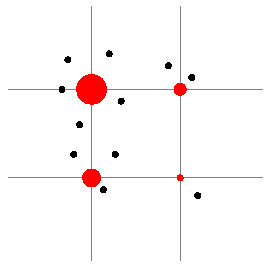
\includegraphics[width=0.35\textwidth]{./img/gridCharge/gridCharge}
	\caption{A schematic representation of the charge assignment. The black filled circles are a unit particle charge, while the red ones, are the charges assigned to grid points. The bigger is the circle, the more is the charge.}
	\label{fig:gidAssign}
\end{SCfigure}

A nice way to solve the problem of charge assignment is to shift the problem to the discretization of the Fourier 
transform. This can be viewed as an interpolation problem. Consider the $e^{-\mathsf{i}\vec k\cdot \vec r_j}$ 
term in the Fourier transform of equation~\eqref{eq:ewaldReciprocal}. In general $\vec r_j$ does not correspond 
to a mesh grid point, so that term is not part of a discrete Fourier transform. The idea, thus, is to interpolate 
it in terms of values of the complex exponential at the mesh points. Switching for simplicity to a one 
dimensional system, if the mesh grid has $M = L/h$ points, a particle coordinate $r_j$ is located between mesh 
points $[r_j/h]$ and $[r_j/h] + 1$ where $[\cdot]$ denotes the integer part; thus a $p$--order interpolation of 
the exponential is of the form
\begin{equation*}
	e^{-\mathsf{i}kr_j} \simeq \sum_{i=1}^M W_{p}\left ( \frac{r_j}{h} - i \right ) e^{-\mathsf{i}khi}
\end{equation*}
where $W_{p}$ denotes the interpolation coefficient. A $p$--order interpolation means that only the $p$ mesh 
points nearest to $r_j$ contribute to the sum. Assuming a point--like charge distribution the Fourier transform 
of the charge density is therefore
\begin{equation*}
	\rho_k \simeq \sum_{i}e^{-\mathsf{i}khi} \sum_j\ q_iW_{p} \left ( \frac{r_j}{h} - i \right )
\end{equation*}
we can interpret the above expression as the discrete Fourier transform of the charge density
\begin{equation*}
	\rho(i) = \sum_j\ q_iW_{p} \left ( \frac{r_j}{h} - i \right )
\end{equation*}
but using equation~\eqref{eq:meshAssign}, it is nothing that the point--like charge distribution assigned to the 
mesh point $i$ through the assignment function $W_{p}$.

We clearly see that the charge assignment problem is now shifted to the complex exponential interpolation. There 
are two main methods to make the interpolation: the \textit{Lagrange interpolation method} and the \textit{Euler 
SPLINE interpolation method}. The basic idea of the former is to use, as interpolating function, a polynomial 
function of degree $ \le (n-1)$ where $n$ is the number of points to interpolate, that passes through all the $n$ 
points, and which is constructed with a summation over the \textit{Lagrange basis polynomials} as follow
\begin{equation*}
	P(x) = \sum_{i=1}^n y_i \prod_{\substack{k=1\\k\ne i}}^n \frac{x-x_k}{x_i - x_k}
\end{equation*}
where $(x_i;y_i)$ are the sets of points to interpolate. The main disadvantage of this method is that, even if 
$P(x)$ is continuous everywhere, its derivative is not, thus it can lead to some instability in \ac{MD} 
simulations.

The latter method, that is the most used in \ac{MD} tools, is based on the concept of \textit{SPLINE 
interpolation}. Instead of using a unique interpolating function that passes through each point, the SPLINE 
method uses a \textit{piecewise polynomial function}, called SPLINE, in which each piece is smoothly connected 
and optimized to interpolate a subset of the points. The Euler SPLINE method use the \textit{exponential Euler 
SPLINE} that is constructed with the basis of the Euler $n$--degree polynomials $A_n(x;\lambda)$ generated by the 
following equation
\begin{equation*}
	\frac{\lambda - 1}{\lambda - e^z}e^{xz} = \sum_{n=0}^{+\infty} \frac{A_n(x;\lambda)}{n!}z^n
\end{equation*}
where $\lambda$ is a complex parameter and $z$ is a complex variable. The main properties of such SPLINE is that, 
it is $n-1$ times analytic, continuously differentiable and then can solve the instability problem of the 
Lagrange interpolation method. In literature the Euler SPLINE method is referred to as \textit{smooth} \ac{PME} 
and the reader is addressed to the article by Essmann \etal\, \cite{EssmannSPME} for more technical details about 
the interpolation procedure.

Summarizing, the \ac{PME} method is implemented with the following scheme
\begin{itemize}
	\item By the interpolation of the complex exponential in the Fourier transform of the Ewald summation, the 
		  Gaussian counteracting charge distribution are spread onto the mesh grid;
	\item Poisson's equation for the discretized charges are solved through the \ac{FFT} methods;
	\item The $U_f$ energy contribution is obtained considering the inverse Fourier transform;
	\item Electrostatic forces are computed and assigned to the charged system particles.
\end{itemize}

The main advantages of the \ac{PME} algorithm are that the potential energy and forces are smooth functions of 
the particles positions. The method offers a good energy conservation and offers a good balance between accuracy 
and computational efficiency since it scales as $\sim N\ln N$. Moreover, despite we have described \ac{ESM} and 
\ac{PME} applied to the electrostatic interaction, they can be used, with some changes, with all long--range 
interactions and in general to all energy contributions that decay as $r^{-d}$, for example, even with the Van 
der Waals energy contribution.

\subsection{Charge representation}
\label{sec:chargeRep}
Even if some methods, such as the \ac{PME} one, have been developed to speed up the computation of electrostatic 
energy contribution one of the main problems of \acp{FF} for biomolecular applications remains the \textit{charge 
representation}: the way in which the charges of atoms or molecules are assigned to the system particles. The 
problem arises from the necessity to represent the electron clouds and the interactions that generate. 
Nevertheless this is crucial for a better description of most electrostatic phenomena such as polarizability of 
molecules and polar solvent, solvation shell of charged ions, protein--ligand interactions, ion transport through 
polar and non--polar medium, self assembly processes and so on.

The most common solution is the \textit{atom--centered ``partial charge'' approximation} in which the full charge 
density of the molecule is replaced by fractional point--like charges assigned to each atom of the molecule. 
Traditionally most non--polarizable \acp{FF} (as those we will use in this thesis work) assign to each atom of a 
molecule a fixed partial--charge. The most used procedure for extracting partial--charges from molecular wave 
functions is based on fitting atomic charges with the molecular electrostatic potential, computed with \textit{ab 
initio} calculation such as \textit{density functional theory}. The fitting procedure consists in minimizing the 
deviation between the electrostatic potential produced by the assigned charge and the molecular electrostatic 
potential. Such representation is believed to be an important source of error in the electrostatics treatment. 
Moreover with fixed charge assignment it is impossible to take into account those phenomena that involve a 
transfer of charge inside the molecule, as polarization effect. The use of off--centered charges and/or higher 
order atomic multipoles can significantly improve the treatment of electrostatics but of course it is necessary a 
good balance between accuracy and performances since the electrostatic problem can rapidly drive to a loss of 
computational efficiency.

\subsection{Polarization}
\label{sec:polarization}
Polarization refers to the redistribution of the electron charge density of a molecule in presence of an external 
electric field, generated, for example, by charged ions or by another molecule. Polarization is responsible to 
non--additive attractive inter-- or intra--molecular interactions which have many--body characteristics. These 
effects have been recognized to have an important role in many biological interactions in which different 
compounds are present. An increasing number of studies show that the lack of these effects can lead to serious 
limitations, particularly, for systems that involve different environments such us water and proteins or water 
and lipids. In \ac{MD} simulations polarization effects are included using either \textit{implicit} or 
\textit{explicit} methods.

The implicit method completely avoids the many--body calculations by including a mean polarization effect in the 
functional form of the interaction potential. The general idea is to surround all the simulation box by a 
transparent medium with a relative dielectric constant $\varepsilon_r$. In this way the polarization effect is 
taken into account considering a mean field theory and solving the Poisson's equation to determine the 
electrostatic potential due to system charges by the substitution 
$\varepsilon_0\rightarrow\varepsilon_0\varepsilon_r$. Since it avoids many--body calculations, this method gives 
an incomparable gain in performances but it must be carefully used. The main disadvantage is that the mean 
polarization effect is added to all system particles and this wash out all the details about a possible 
polarization effect in a molecule. Moreover the electrostatic interaction between charged particles is affected 
by the mean field effect. This produce a correct electrostatic interaction for particles inside the same solvent 
for which the implicit medium is parameterized. Otherwise, if the simulation box is composed by different 
chemical environments such as a polar and non--polar compounds, using the same dielectric constant would lead to 
badly calculate the electrostatic interactions for particles in the non--polar environment. Thus, this method can 
be safely used when our system is composed principally by one kind of solvent, for example water. 

The way to correct the above behavior is to use an explicit method. As the name suggests, the polarization effect 
is taken into account for every molecule in the system by an its proper model included in the \ac{FF}. The 
general idea is to add some more internal \ac{DOF} to a molecule or atom to take into account the movement of 
charges and/or split the point--like charge assigned, for example, to a chemical group, to a partial-charge 
assigned to each particles of the chemical group itself. This can be done for every molecule or atom in the 
system and thus it is the optimum to better describe systems with different chemical environments. Obviously this 
method is more time consuming compared to the first. 

%\subsection{Atomistic model}
\subsection{Coarse--Grained model}
\label{sec:CGModel}
As we have introduced at the beginning of this section, for biomolecular applications two main classes of 
classical \acp{FF} exist: atomistic \acp{FF} and \ac{CG} \acp{FF}. Since the atomistic model takes into account 
all the atoms in a molecule it is obviously the most realist and accurate \ac{FF}. Nevertheless the large number 
of \ac{DOF} of atomistic \acp{FF} leads to a loss of computational performance. Moreover, basically, the 
atomistic \acp{FF} are efficient until the physical proprieties can be properly sampled on a time scale of a few 
microseconds over a length scale of a few nanometers. As the time and length scales increase more and more time 
is needed to carry out a complete simulation. Unfortunately many biological processes involving lipid membranes 
and other organic molecules, including synthetic compounds, take place on much longer time and length scales.

One possible solution is to \textit{integrate out} some \ac{DOF}, preserving those that are relevant for the 
problem in exam: this procedure is called \textit{coarse--graining}. The basic units of \ac{CG} \acp{FF} are 
called \textit{beads}, each representing a group of atoms or a well defined chemical moiety. The size of the 
group of atoms that is represented by a single bead determines the degree of coarsening of the \ac{FF}. Even in 
this case, all the general features described above, apply: functional forms need to be chosen and their 
parameterization need to be adjusted so as to reproduce the desired target properties. 

The first step in the development of a \ac{CG} model is the \textit{mapping} procedure. This establishes a link 
between the atomistic model and the \ac{CG} one. There is not a unique or correct procedure to perform the 
mapping because it depends on the desired coarse--graining level, on the time and length scales that one wants to 
correctly sample and on the properties one wants to reproduce. For biological applications \ac{CG} \acp{FF} are 
often designed to reproduce specific thermodynamic properties such as surface tension, free energy of 
partitioning, free energy of hydration and so on. \ac{CG} \acp{FF} employed in the of material sciences (e.g. 
polymer science) often use as a target the material structural properties.

In general a \ac{CG} \ac{FF} is more computationally efficient than an atomistic one for the following reasons
\begin{itemize}
\item the \ac{DOF} of the system are reduced due to the \ac{CG} procedure with the consequence that a smaller number of interactions and forces has to be computed;
\item bead--bead interactions, which result from the removal of finer structural details, are softer than atom--atom interactions;
\item vibrational modes are slower, and their sampling can be achieved using larger \ac{MD} time steps than in atomistic simulations;
\item softer interactions imply a smoother \ac{PEF} which leads to faster diffusion.
\end{itemize}

\section{MARTINI: a Coarse--Grained Force--Field}
\label{sec:martini}
\martini is a \ac{CG} \ac{FF} developed by Marrink \etal\, \cite{Martini} for organic solvents and lipids and 
then extended to proteins \cite{MartiniProtein}, carbohydrates \cite{MartiniCarbo} and a broad class of polymers 
\cite{MartiniPolymers}. \martini is based on a chemical building block approach. Such \martini blocks or beads 
represent small chemical moieties and they are extensively calibrated in order to construct a large variety of 
organic molecules. As we shall see in section~\ref{sec:martiniParam}, the \ac{FF} is based on accurately 
reproducing the interaction between polar and non--polar chemical compounds. The main target property is intact 
the \textit{partitioning free energy} between water and a large number of organic solvents, i.e. the free energy 
of transfer of chemical moieties from polar and non--polar solvents.

\subsection{Mapping}
The mapping of the \martini beads is based on a four--to--one scheme that groups four heavy atoms like C, S, O 
and so on, plus their associated hydrogen atoms, into a single interaction site. Consistently four water 
molecules are modeled with one \martini bead. An example of the mapping procedure including both atomistic and 
\ac{CG} descriptions is shown in figure~(\ref{fig:martiniMapping}).
\begin{figure}[!ht]
	\centering
	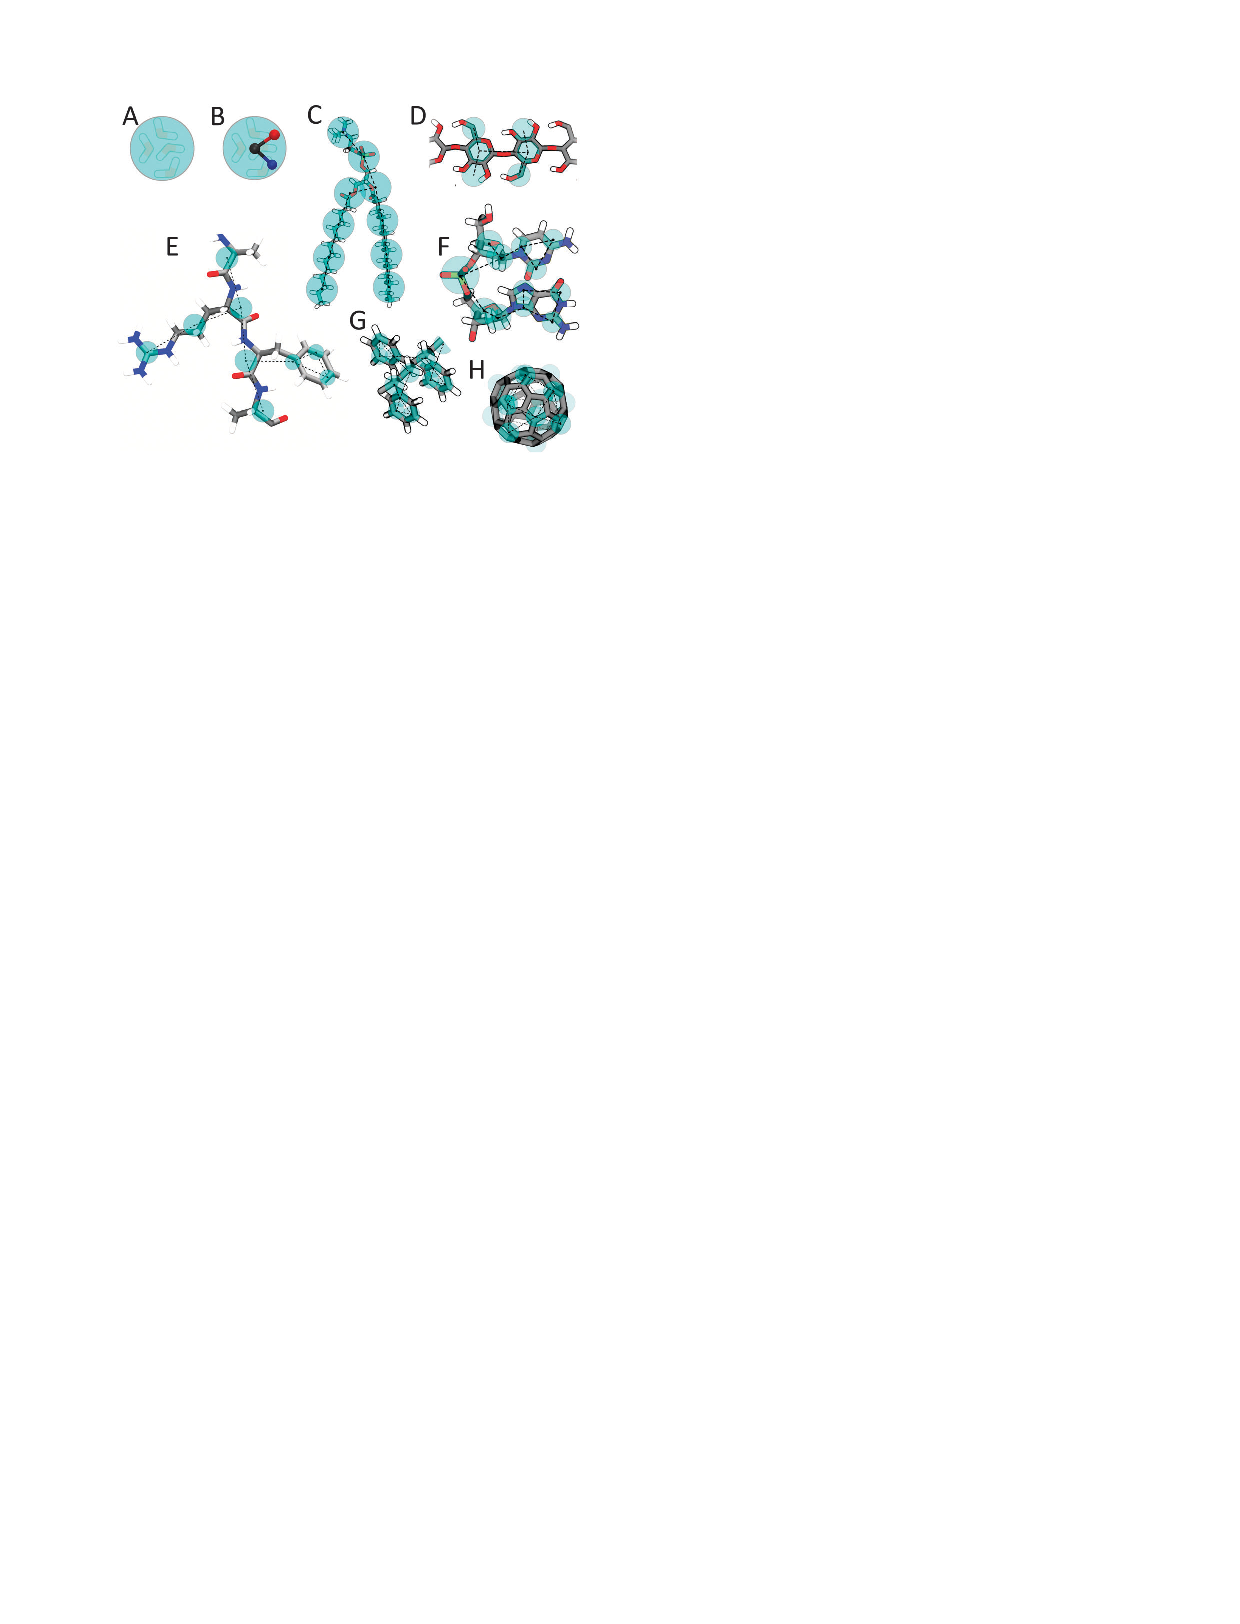
\includegraphics[width=0.5\textwidth]{img/martiniMapping}
	\caption{\martini mapping and atomistic structures compares of some molecules: (A) Standard water bead, (B) polarizable water bead, (C) \acs{DMPC} lipid, (D) Polysaccharide fragment, (E) Peptide, (F) DNA fragment, (G) Polystyrene fragment and (H) Fullerene molecule. In all cases \martini \acs{CG} beads are shown as cyan transparent beads overlaying the atomistic structure. Taken from \cite{MartiniReview}.}
	\label{fig:martiniMapping}
\end{figure}

There are four main bead types: polar (P), non--polar (N), apolar (A) and charged (Q). Each bead type has a 
number of subtypes to take into account a more accurate representation of the chemical nature of the moieties due 
to the underlying specific atomistic structure. These subtypes are distinguished by the hydrogen bonding 
capabilities: donor (d), acceptor (a), both donor and acceptor (da) and none ($0$) and/or by their degree of 
polarity: lowest polarity ($1$), $\dots$, highest polarity ($5$).

\begin{SCtable}\footnotesize
	\begin{tabular}{lc}
		\toprule
		Level  & $\epsilon$\,[kJ/mol] \\ \midrule
		O	   & $5.6$	 \\ \midrule
		I      & $5.0$	 \\ \midrule
		II	   & $4.5$	 \\ \midrule
		III	   & $4.0$	 \\ \midrule
		IV	   & $3.5$	 \\ \midrule
		V	   & $3.1$	 \\ \midrule
		VI	   & $2.7$	 \\ \midrule
		VII	   & $2.3$	 \\ \midrule
		VIII   & $2.0$	 \\ \midrule
		IX     & $2.0$	 \\ \bottomrule
	\end{tabular}
	\caption{Interaction strength parameter ($\epsilon$). The last one is for the special case $\sigma=0.62$~nm.}
	\label{tab:martiniEpsilon}
\end{SCtable}

\subsection{Interactions potential}
\label{sec:martiniPotential}
\paragraph{\textbf{van der waals interactions}} The functional form describing pairwise Van der Waals interaction 
is a Lennard--Jones $12-6$ potential as in equation~\eqref{eq:lj126}. For most beads the $\sigma$ parameter is 
set equal to $0.47~$nm except for the Q--C$_1$ and Q--C$_2$ interactions for which $\sigma = 0.62$~nm. This is 
consistent with reproducing the hydration shell when a charged bead (Q) is dragged into an apolar medium. The 
strength of the interactions is instead dived into ten levels, reported in table~(\ref{tab:martiniEpsilon}). The 
association of the interaction strength with each \martini beads is shown in 
figure~(\ref{fig:martiniInteractions}).
\begin{figure}[h!t]%
	\center
	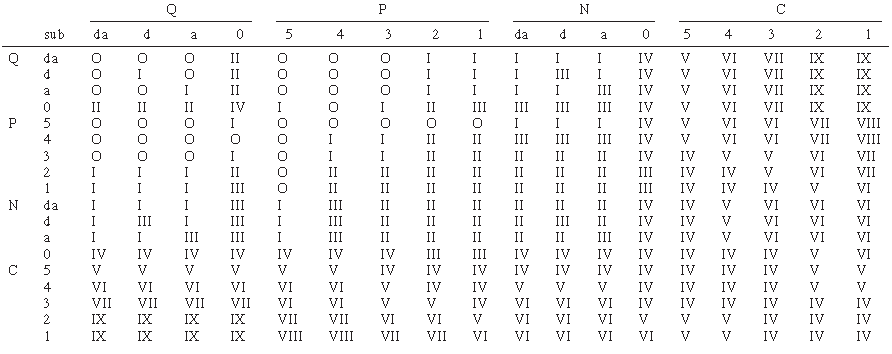
\includegraphics[width=\textwidth]{img/martiniInteractions.pdf}%
	\caption{Interaction strength association matrix for the \martini bead types and subtypes. Taken from \cite{Martini}.}
	\label{fig:martiniInteractions}
\end{figure}

\paragraph{\textbf{electrostatic interactions}} Electrostatic charges are assigned using the atom--centered 
approximation, as described in~\ref{sec:chargeRep}. The charges of the \martini beads are empirically assigned at 
the center of the beads and correspond to the net charge of the chemical moiety they represent. Water, for 
example, is described by a neutral P$_4$ beads. Van der Waals interactions are responsible for take into account, 
effectively, the effects of polarizability together with the use of an implicit medium with a dielectric constant 
$\varepsilon_r = 15$. However, as we shall see in section~\ref{sec:pw}, to avoid the problems with the implicit 
medium described in~\ref{sec:polarization}, especially for lipid membranes for which the dielectric constant in 
the hydrophobic region is much smaller, Yesylevskyy \etal\, \cite{PW} have developed a more sophisticated \ac{CG} 
water model, called \ac{PW}, to take into account a better water behavior.

\paragraph{\textbf{bonded interactions}} They include only bond length and an angle harmonic contributions. The 
former is modeled with a harmonic potential as the first term in equation~\eqref{eq:bondPEF}, with the same bond 
constant for all bead types: $k^b = 1250$~kJ/(mol\ nm$^2$) and an equilibrium distance of $l_0 = 0.47$~nm. The 
latter is modeled as a cosine--type harmonic potential
\begin{equation}
	U = \frac{1}{2}k^a (\cos(\theta) - \cos(\theta_0))^2
	\label{eq:martiniAngle}
\end{equation}
whose parameters are: $k^a = 25$~kJ/mol and $\theta_0 = 180^\circ$ for aliphatic chains; $k^a = 45$~kJ/mol and 
$\theta_0 = 120^\circ$ for \texttt{cis} double bonds and $k^a = 45$~kJ/mol and $\theta_0 = 180^\circ$ for 
\texttt{trans} unsaturated bonds. Moreover, especially for ring systems, an improper dihedral angle harmonic 
potential can be used to prevent out of plane distortion. The form is
\begin{equation*}
	U = k_{id} (\theta_{ijkl} - \theta_0)^2
\end{equation*}
where $\theta_{ijkl}$ denotes the angle between the planes described by atoms $i,j,k$ and $j,k,l$; $k_{id}$ and 
$\theta_0$ are, as usual, the force constant and equilibrium angle.

\subsection{Simulation parameters}
The \martini \ac{FF} was originally developed using a shifted cut--off scheme for both Lennard--Jones and 
electrostatic potentials with a cut--off radius $r_c = 1.2$~nm. The Lennard--Jones potential was shifted from 
$r_s = 0.9$~nm to $r_c$ while from $r_s = 0.0$~nm to $r_c$ for the electrostatic potential. The neighbor list is 
constructed as described in the first part of~\ref{sec:neighbor} with a refresh rate of $10$ \ac{MD} steps. 
Recently the more efficient Verlet cut--off scheme was tested by Marrink \etal\, \cite{MartiniReview} and used 
with the \martini \ac{FF} with a cut--off radius of $r_c = 1.1$~nm, a Verlet buffer tolerance of $0.005$~kJ/(mol\ 
ps) and a minimum refresh rate of $10$ \ac{MD} steps (often, depending on the hardware, it can be dynamically 
increased to $30$ or $40$ \ac{MD} steps getting better performances).  Moreover, the treatment of the 
electrostatic interaction can be safely updated to the \ac{PME} method together with the Verlet cut--off scheme. 
This new set--up was largely tested by Yesylevskyy \etal\, \cite{PW}. In this case the cut--off radius was set to 
$r_c = 1.2$~nm with the same Verlet buffer tolerance; the \ac{PME} grid spacing was set to have a lower bound of 
$0.12$~nm and the interpolation was set to a fourth-order. Moreover, with the use of \ac{PW}, as we shall see, 
the dielectric constant should be reduced to $\varepsilon_r = 2.5$. In all cases a time step 
$20\le\delta t\le 40$ is suitable for a great number of applications. It should be clear that changing these 
simulation parameters must be followed by a retest of the main properties of the \martini \ac{FF}.

\subsection{Parametrization}
\label{sec:martiniParam}
In order to parametrize the \martini \ac{CG} \ac{FF} a set of thermodynamics properties, obtained from \ac{MD} 
simulations, are compared and fitted against those experimentally measured. These properties are the \textit{free 
energies of vaporization}, \textit{hydration} and \textit{partitioning} between water and a set of organic 
compounds such as hexadecane (H), chloroform (C), ether (E) and octanol (O). The free energy of hydration was 
obtained from the partitioning of \ac{CG} beads between bulk water in equilibrium with its vapor. Similarly the 
free energy of vaporization was obtained considering a simulation box with the selected \ac{CG} bead in a liquid 
phase in equilibrium with its vapor. From the equilibrium densities of the particles in both phases the related 
free energies can be computed from
\begin{equation*}
	\Delta G = k_B T\ln \left ( \frac{\rho_{\text{vap}}}{\rho_{\text{bulk}}} \right )
\end{equation*}
All the simulations were performed in a canonical $NVT$ ensemble.

The partitioning free energy between water and an organic solvent was obtained in a $NPT$ ensemble, considering a 
simulation box half filled of water and half of the organic solvent. Then a small fraction of the \ac{CG} 
particle for which the partitioning free energy is to be computed, was placed in the simulation box. From the 
equilibrium densities of the particles in water $\rho_{\text{wat}}$ and in organic solvent $\rho_{\text{oil}}$, 
the free energy of transfer can be computed from
\begin{equation*}
	\Delta G_{SW}^{\text{part}} = k_B T \ln \left ( \frac{\rho_{\text{oil}}}{\rho_{\text{wat}}}\right )
\end{equation*}
where $S$ indicate the organic solvent.

In figure~(\ref{fig:martiniTarget}) a summary of the results is reported. As one can see the model has bad 
performances for what concerns the free energies of vaporization and hydration, which are too high with respect 
to experimental data. Instead, the partitioning free energies match very well. Thus the model is not very 
accurate for vapor--liquid systems but it is reliable at describing the behavior of liquid phases with 
different degrees of hydrophobicity.
\begin{figure}[h!t]%
	\center
	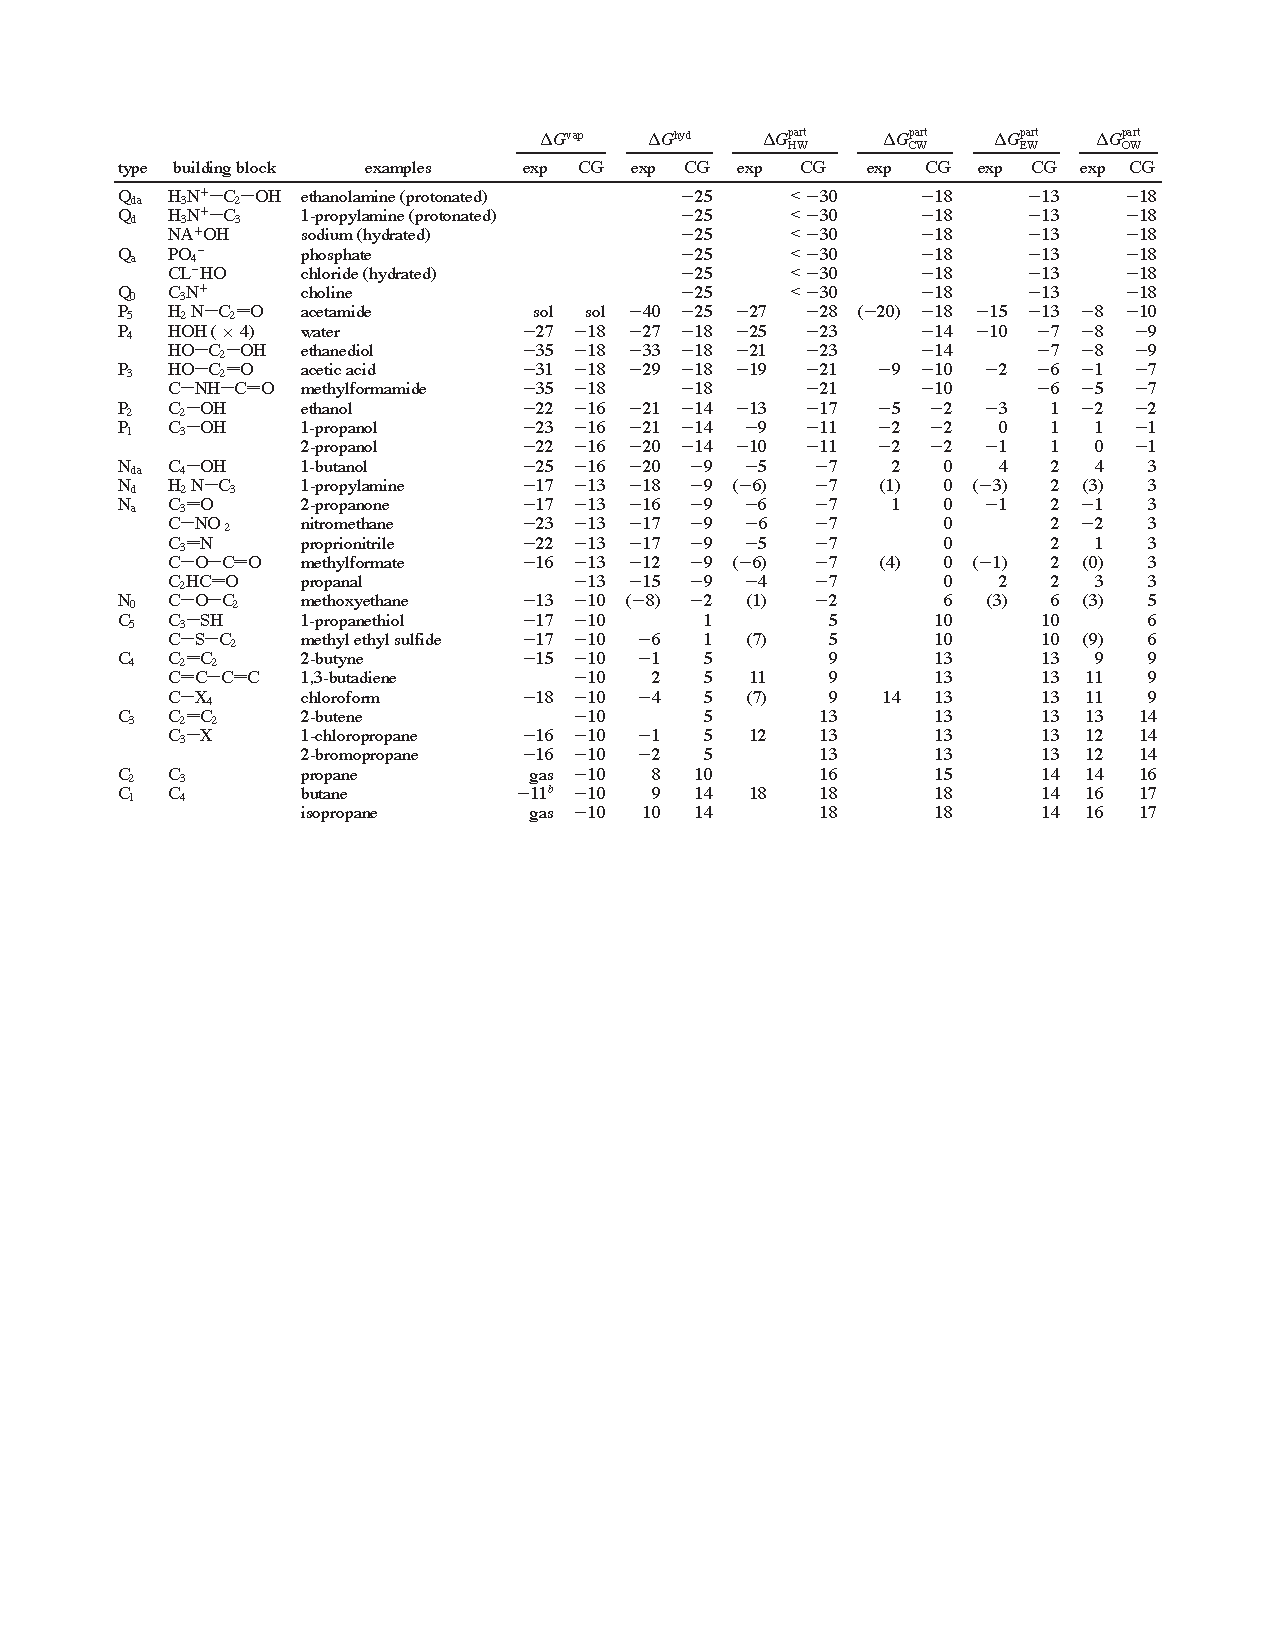
\includegraphics[width=\textwidth]{img/martiniTarget}%
	\caption{Results summary: free energies of vaporization $\Delta G^\text{vap}$, hydration $\Delta G^\text{hydr}$ and partitioning $\Delta G^\text{part}$ between water (W) and organic solvents (hexadecane (H), chloroform (C), ether (E) and octanol(O)) compared to experimental values. Experimental properties in parentheses are estimates obtained from comparison to similar compounds. The statistical accuracy of the free energies obtained from the simulations is $\pm 1$~kJ/mol. $^b$ The temperature for the experimental data is $273$~K. Taken from \cite{Martini}.}
	\label{fig:martiniTarget}
\end{figure}

\subsection{Polarizable Water model}
\label{sec:pw}
Water plays a crucial role in any biomolecular system. It is important thus to correctly describe its behavior. 
Since the \martini water model does not directly take into account the electrostatic interaction between water 
and water and other environment because it does not have any charge and it interact only via Van der Waals 
interaction, a simple implicit medium is used to take into account the main electrostatic effects of water, 
screening and polarizability. In reality, however, any biomolecular process involves charged species moving 
between regions of different dielectric constant. Due to the change in electrostatic screening between those 
environments, the strength of the interaction between the moving charges and the surrounding molecules also 
changes. This effect can not be taken into account by implicit medium models. In order to capture the 
inhomogeneous nature of the dielectric response an explicit medium has to be used. 
\begin{figure}[!ht]
	\centering
	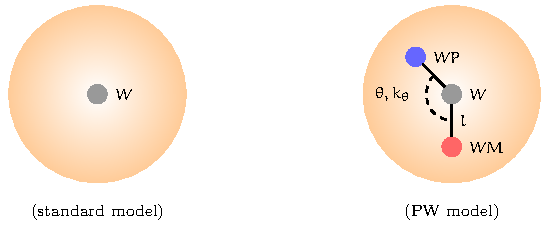
\includegraphics[width=0.7\textwidth]{./img/PWModel/PWModel}
	\caption{Schematic representation of the \acs{PW} bead. Shaded orange spheres correspond to the Van der Walls radii of the central neutral particle $W$. The blue particle is the positively charged while the red is the negatively charged.}
	\label{fig:PW}
\end{figure}

In the same fashion of the \martini philosophy, Yesylevskyy \etal\, \cite{PW} have developed a \acf{PW} model 
that better describes the real behavior of water. As before one \ac{PW} bead is associated to four water 
molecules. The new water bead consists of three particles instead of one in the standard \martini model. In 
figure~(\ref{fig:PW}) the topology of the \ac{PW} and a comparison with the old model is shown. The central 
particle $W$ is neutral and interacts with other particles in the system with the only Lennard--Jones potential, 
just like the standard P$_4$ water bead (see figure~(\ref{fig:martiniInteractions}) for the interactions matrix). 
There are two additional particles, namely $WP$ and $WM$, that are bound to the central particle and carry a 
positive and negative charge $|q| = 0.46\mathsf{e}$ respectively, where 
$\mathsf{e} = 1.60217653(14) \cdot 10^{-19}$~C is the unit electron charge. They interact with other particles in 
the system by the Coulomb interaction only. The bonds $W-WP$ and $W-WM$ are constrained to have a fixed distance 
$l = 0.14$~nm. The electrostatic interaction between $WP$ and $WM$ inside the same bead are exclude, thus they 
are invisible to each other and they can rotate around the $W$ particle. As a consequence the dipole momentum of 
the water bead depends on the relative angular position $\theta$ of $WP$ and $WM$: it can vary from zero 
($\theta = 0$) to $2ql$ ($\theta = \pi$). A harmonic angle potential with equilibrium angle fixed to 
$\theta_0 = 0$ and a force constant $k_\theta = 4.2$~kJ/(mol\ rad$^2$) is added to control the rotation of 
$WP$ and $WM$ particles around the $W$ particle, so to adjust the distribution of the dipole momentum. The value 
of the equilibrium angle is consistent with the fact that in an apolar medium the total dipole momentum of a 
water molecule is zero. 

Since in this model the screening and polarization effects are treated explicitly the global dielectric constant 
is then reduced from $\varepsilon_r = 15$, used in the standard \martini, to $\varepsilon_r = 2.5$. Moreover, 
since the \ac{PW} beads attract each other stronger then the standard water beads, because of the additional 
electrostatic interactions, the strength $\epsilon_{WW}$ of the Lennard--Jones interaction between $W$ particles 
must be reduced. Water properties are reproduced satisfactory if the Lennard--Jones strength is changed from an 
$I$ level to an $III$ level (see table~(\ref{tab:martiniEpsilon}) for the various interaction levels). $\sigma$ 
remains set to $0.47$~nm. The same apply with the Lennard--Jones interactions between Q type beads and other 
beads. For recover the correct partitioning behavior the strength of such interactions are modify according to 
figure~(\ref{fig:PWMartini})
\begin{figure}[!ht]
	\centering
	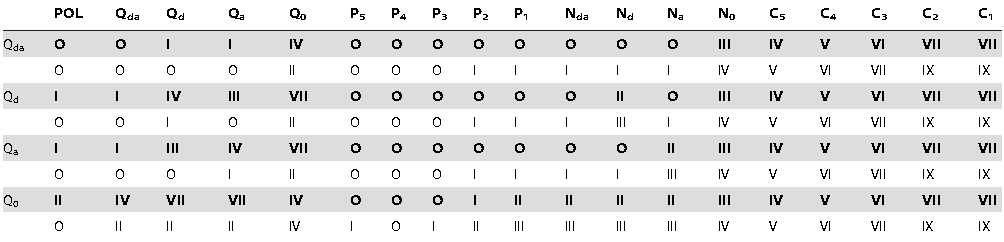
\includegraphics[width=\textwidth]{./img/PWMartini}
	\caption{New interaction strength between Q type beads and other beads. New values in bold font, old values in normal font. See table~(\ref{tab:martiniEpsilon}) for the interaction levels. Taken from \cite{PW}.}
	\label{fig:PWMartini}
\end{figure}

The parametrization of $q$, $k_\theta$ and $\epsilon_{WW}$ are obtained, in addition to the basic target 
properties of the \martini \ac{FF}, also trying to reproduce the dielectric constant $\varepsilon_{W}$, density 
$\rho$ and dipole momentum of a pure water phase. The above parameters of the \ac{PW} model are summarized in 
table~(\ref{tab:PWParam}) while a comparison of the results obtained with the \ac{PW}, the standard \martini 
water and the experimental data are summarized in table~(\ref{tab:PWRes}). For more details about the 
parameterizations and testing methods the reader is 
addressed to the article by Yesylevskyy \etal\,\cite{PW}.
\begin{SCtable}
	\centering
	\begin{tabular}{ll}
		\toprule
		$|q| = 0.46\mathsf{e}$				\\ \midrule
		$l = 0.14$~nm						\\ \midrule
		$\theta_0 = 0$						\\ \midrule
		$k_\theta = 4.2$~kJ/(mol\ rad$^2$)	\\ \midrule
		$\epsilon_{WW} = 4$~kJ/mol			\\ \midrule
		$\sigma = 0.47$~nm					\\ \bottomrule
	\end{tabular}
	\caption{Summary of the parameters used in the \acs{PW} model. Taken from \cite{PW}.}
	\label{tab:PWParam}
\end{SCtable}

\begin{table}
	\centering
	\begin{tabular}{lrrr}
		\toprule
		\,	& \acs{PW} &  \martini water & Experimental \\ \toprule
		$\rho$~[kg/m$^3$]				& $1043$  &   		& $997$		\\ \midrule
		$\overline{p}$~[D] 				& $4.9$   & $-$ 	& 		    \\ \midrule
		$\varepsilon_{W}$ 				& $75.6$  & $-$ 	& $78.4$	\\ \midrule
		$T_\text{melt}$~[K] 			& $282$   & $290$ 	& $273$		\\ \midrule
		$\Delta G^\text{hyd}$~[kJ/mol] 	& $-18.7$ &	$-18$	& $-27$		\\ \midrule%\subsection{Applications}
		$D_{WW}~[10^{-5}$~cm$^2$/s]		& $2.5$   & $2.0$   & $2.3$		\\ \bottomrule
	\end{tabular}
	\caption{Summary of the results obtained with the \acs{PW}, standard \martini water and the experimental data at $T=300$~K. $\overline{p}$ is the average dipole momentum and $D_{WW}$ is the self--diffusion coefficient.}
	\label{tab:PWRes}
\end{table}

Moreover, the authors found that, in addition to the \ac{PW} model, the use of \ac{PME} method contributes to a 
more realistic description of the processes involved in biomolecular environments. In particular, some 
interesting results of utility for this thesis work concern a better description of the properties of lipid 
membranes, as we shall see in Chapter~\ref{chap:tre}.
%One is the translocation of charged ions through a lipid bilayer that is described in a more realistic detail: the authors found that the simulations with \ac{PW} and \ac{PME} are approaching the atomistic results better then the standard \martini \ac{FF}. Another important phenomenon about lipid membranes consist in the electroporation of membrane by \ac{PW} beads due to an electric field across the membrane (for example, created by a cross membrane ions imbalance) and, related to this, the translocation of ions across the membrane helped by a so called ``\textit{water finger}'' a water defect inside the membrane that seems to be the trigger of the ions translocation. Such phenomenons are clearly evident in atomistic simulations however never occurred using the standard \martini \ac{FF} thus the importance to use the \ac{PW} model together with \ac{PME} method.
			
\subsection{Limitations of MARTINI FF}
As we have seen in~\ref{sec:CGModel} the \ac{CG} \acp{FF} are computationally advantageous, still a price has to 
be paid. Although the \martini \ac{FF} is still a fine \ac{CG} \ac{FF}, some limitations are shared with other 
\ac{CG} models at a fundamental level, such as the chemical and spatial resolution, which are both limited 
compared to atomistic models. An important issue is the underestimation of the entropy which respect to the 
atomistic case, that is a consequence of the \ac{DOF} reduction process. Since in the \martini \ac{FF} the 
partitioning free energy $\Delta G = \Delta H - T\Delta S$ must be consistent which the experimental data, the 
intrinsic loss of entropy imply a reduction of the enthalpy contribution, generating an imbalance between them. 
If a $NVT$ ensemble is used the correct potential is the Helmholtz free energy $\Delta A = \Delta U - T\Delta S$, 
thus the imbalance is between the internal energy and the entropy. This means that the use of a \ac{CG} model 
with a $NVE$ ensemble leads to a problem of energy conservation. Anyway this is not our case since we only use a 
$NVT$ or a $NPT$ ensemble with an external thermostat coupling.

Another consequence of the use of a \ac{CG} \acp{FF} is related to the \ac{FES} that becomes smoother respect to 
the atomistic case. This effectively results in more sampling of the energy landscape in a given time period, 
speeding up the dynamics of the system. Moreover even the \ac{PEF} becomes smoother, in particular the bonded 
contributions, allowing the use of an higher time steps with longer simulation times. However the speed--up is 
not easily predictable and is not likely to be the same for different systems and maybe it is dependent on the 
type of molecule. Nevertheless for the \martini \ac{FF} an average scaling factor of four, based on lateral 
diffusion coefficients of lipids in membranes, is commonly used, of course with some care. Another smaller source 
of errors is due to the choice of masses: since ensemble properties are not affected by particle masses, in order 
to increase the efficiency, all the \martini beads have the same mass of $72$~amu. This leads in some uncertainty 
in the dynamics of the system making the time scaling for different beads non--trivial.

A problem involving the Lennard--Jones potential as a model of Van der Waals interactions in \martini, is that 
the steep repulsion leads to an over--structuring of fluids compared to atomistic models. As we can see from 
table~(\ref{tab:PWRes}) the direct and most evident implication is the melting point of the standard \martini 
water that is $290 \pm 5$~K. A practical partial solution is the use of the so called ``anti--freeze'' particles 
named BP$_4$ type. The Lennard--Jones interaction between these particles and water is modified with a slightly 
larger Van der Waals radius parameter, $\sigma = 0.57$~nm and a stronger interaction to be a level $O$ (see 
table~(\ref{tab:martiniEpsilon}) for the interaction level). Marrink \etal\, suggest that a mole fraction of 
$n_{\text{af}} = 0.1$ is sufficient to prevent freezing without affecting the other properties of water. 
%Some other properties of water are not accurate described such us the surface tension of air/water interface that leads in problem to water/oil interfaces formation. 
Using the \ac{PW} model these properties improve slightly, see table~(\ref{tab:PWRes}). For a more comprehensive 
discussion about the limitations of the \martini \ac{FF} the reader is addressed to the review by Marrink \etal\, \cite{MartiniReview}.

\section{Advanced sampling methods}
The Gibbs (or Helmholtz) free energy function is a quantity of particular importance for the equilibrium 
statistical mechanics of which we are interested to obtain with \ac{MD} technique. In fact, the time evolution of 
a biomolecular system and its equilibrium properties are determined by the system's \ac{FES}. This because free 
energy differences tell us, for example, if a chemical reaction occurs spontaneously, whether a given solute is 
hydrophobic or hydrophilic, if a protein conformational change can take place or whether some molecules in water 
solution are able to self--assemble into a more complex system and so forth. Being related to the partition 
function of an ensemble, the free energy is the generator through which other thermodynamic quantities are 
obtained via differentiation. However often we are particularly interested in the free energy difference between 
two thermodynamic states, instead of the absolute value. The Gibbs free energy $G$ is specific for the $NPT$ 
isobaric--isothermal ensemble and the Helmholtz free energy $A$ for the $NVE$ canonical ensemble. 

\paragraph{\textbf{Collective variables}} Often, we are interested in the \ac{FES} in function of some 
generalized coordinates, called \acp{CV} of the system. These small set of variables can describe, in a simple 
and useful manner, some chemical, thermodynamic or mechanical processes that take place in the system. For 
example, the free energy in function of the distance between the \ac{COM} of two molecules give us information 
about their attraction or repulsion and if they form a bound state. Thus the \ac{FES}, in the \acp{CV} space, 
provides a map of the stable conformations, the relative stability of these conformations and the barrier heights 
that must be crossed for the processes to take place. Moreover, the energy landscape, even for a small molecule, 
can be extremely wrinkled and the large number of minima can not be sampled in a typical \ac{MD} simulation. The 
principal reason for the use of the \acp{CV}, is thus to limit the sampling to those regions of phase space that 
are most important for the process under study, hoping that the limited sampled regions are sufficient to 
correctly describe the process.
%It is necessary to stress out that in many cases one do not know exactly \textit{a priori} the \ac{FES} about a certain process and so one want to know it also for understand if other minima energy configurations exist, in addition to those known, how stable they are and what are the energy barriers to go from one minima state to an other\footnote{Sometimes thought the cinematic of an \ac{MD} simulation one can gamble an estimate of the functional form of the \ac{FES}, looking for the relative probability to stay in a meta--stable state rather then the other. Clearly this means that both meta--stable states are to be sampled, as we shall see later it depends of the height of the energy barriers.}. 

\paragraph{\textbf{Free energy surface}} The calculation of free energy difference between two thermodynamic 
states (that requires an \textit{a priori} knowledge of the two stable states) and the calculation of the 
\ac{FES} are one of the main challenges in \ac{MD} simulations for biomolecular applications. Let us suppose that 
we are interested in the \ac{FES} in function of the \ac{CV} $s(\vec r)$ and we are working in a $NPT$ 
ensemble\footnote{The following is still valid even for a $NVE$ ensemble with the substitution $G\rightarrow A$ 
and the use of the correct partition function $\mathcal{Z}_{NVE}$.} with an isotropic system. Following 
section~\ref{sec:statmec}, the Gibbs free energy along the \ac{CV} is obtained as
\begin{equation}
	G(s) = -k_BT \ln Q(s)
	\label{eq:fes}
\end{equation}
where $Q(s)$ is the partition function that integrate out all the \ac{DOF} of the system expect for $s(\vec r)$:
\begin{equation*}
	Q(s) = \frac{1}{\mathcal{Z}_{NpT}} \int_0^{+\infty}\ dV \ \int_\Omega e^{-\beta(\mathcal{H}(\vec x) + pV)}\delta(s(\vec r) - s)\ dx
\end{equation*}
since $s(\vec r)$ does not depend on particle momenta, from equations~\eqref{eq:hamiltonian} 
and~\eqref{eq:nptPartition}, $Q(s)$ can be rewritten as
\begin{equation}
	Q(s) =  \frac{ \int_\Omega e^{-\beta U(\vec r)}\delta(s(\vec r) - s)\ dr }{\int_\Omega e^{-\beta U(\vec r)}\ dr}
	\label{eq:CVprobability}
\end{equation}
where $U(\vec r)$ is the \ac{PEF}. $Q(s)ds$ can be interpreted as the probability to find the system with 
$s(\vec x)$ between $s$ and $s + ds$. Since this equation contains a direct phase space integration it can be 
rewritten in a more useful manner using the ensemble averages and then, using the ergodic theorem in 
equation~\eqref{eq:ergotic}, as a time average:
\begin{equation}
	Q(s) = \ave{\delta(s(\vec r) - s)} = \lim_{t\to +\infty}\frac{1}{\tau}\int_0^\tau \delta(s(\vec r(t)) - s)\ dt
	\label{eq:CVprobabilityAve}
\end{equation}

The time sampling of equation~\eqref{eq:CVprobabilityAve} can be 
derived, in principle, via \ac{MD}. Unfortunately, since the time can not be infinite, the main problem related 
to \ac{MD} simulations is whether we are able to correctly sample \textit{all} the phase space of an ensemble in 
order to compute the ensemble average. Clearly the answer depends on the system in exam, if it is really simple 
maybe we can do that, otherwise probably not or indeed it take too much time and/or we are not able to collect 
sufficient data. This sampling problem can be summarized as follows: regions in phase space around a local 
minimum of the \ac{FES} are typically sampled well, whereas regions of higher energy are sampled rarely. These 
high energy regions provide with a small contribution to the partition function, due to their unfavorable 
Boltzmann factor. However they must be overcome in order to sample other minima that can give, instead, a 
important contribution to the ensemble averages. These transitions are called \textit{rare events}. When the 
system is moving in the energy landscape the only way to escape from a local minimum is to exploit thermal 
fluctuations and so energy barriers that are higher then $\sim k_B T$ have a small probability of being overcome. 

\paragraph{\textbf{Bias based advanced sampling}} Several methods are developed and are still in development in 
order to solve the just described sampling problem. These methods are all based on advanced sampling techniques 
that allow us to
\begin{itemize}
	\item Escape from a local energy minimum, in order to explore other regions of the phase space;
	\item Calculate the free energy difference between two thermodynamic states;
	\item Compute the \ac{FES} along one or a small set of \acp{CV}.
\end{itemize}
The common basic idea is to introduce a additional \textit{bias potential} able to confine the sampling to a 
limited region of the \ac{CV} space and/or drive the transition between two metastable configuration. In 
particular we describe only those methods used in this thesis work: \textit{umbrella sampling method} and 
\textit{metadynamics}. For a more comprehensive discussion the reader is addressed to the review by Kästner 
\cite{Umbrella} for the former, and to the review by Laio and Gervasio \cite{MetadReview} for the latter. 
Moreover in the books by Tuckerman \cite{Tuckerman} other enhanced sampling methods are described.

\subsection{Umbrella sampling}
The umbrella sampling method was developed by Torrie and Valleau and today is one of the most mature and broadly 
accepted method for calculating free energy differences. The basic idea is to drive the system from a known state 
$A$ to an other known state $B$ through a deterministic path defined on the \ac{CV} $s(\vec r)$ chosen to 
describe the process. This method is well suited for one \ac{CV}, otherwise the computational performance 
degrades rapidly with the number of \acp{CV}. The idea is to identify a path connecting $A$ to $B$, and divide it 
into a discrete number of windows $N_w$ and take a subset $\{s_i\}$, $i=1,\dots,N_w$ of the values assumed by the 
continuos \ac{CV} from state $A$ to $B$ along the path. For each of these target values $s_i$ a bias potential 
$w_i(s)$, depending only on $s$, is added to \ac{PEF} in order to restrain the system to the $s_i$ target value. 
Then, \ac{MD} simulations are performed for each window. All the data collected within the $N_w$ windows are 
combined together to compute the biased \ac{FES} along the chosen \ac{CV}. Eventually, the unbiased \ac{FES} is 
recovered. In figure~(\ref{fig:umbrellaPath}) an example of the windows selection is shown.
\begin{SCfigure}
	\centering
	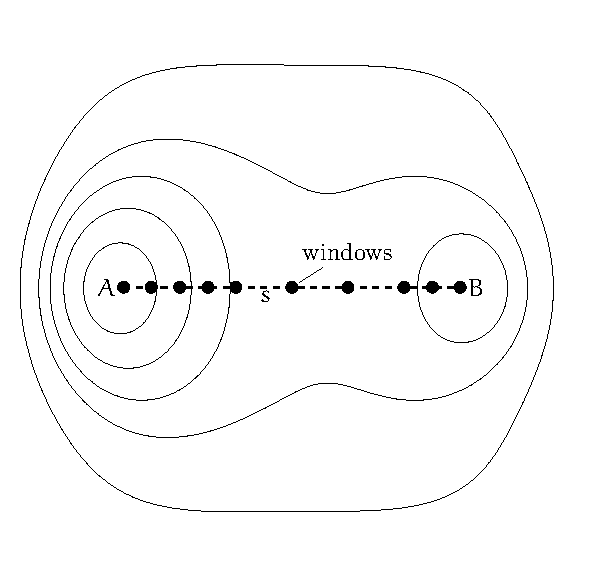
\includegraphics[width=0.5\textwidth]{./img/umbrellaPath/umbrellaPath.pdf}
	\caption{Example of an umbrella sampling windows selection. The contour plot represent a $2$--minima free energy profile through which the system is evolved. The dashed line is the path along the \acs{CV} $s(\vec r)$ that connect state $A$ to $B$. The black filled circles represent the selected windows for different values of $s$.}
	\label{fig:umbrellaPath}
\end{SCfigure}

Suppose $w_i(s)$ to be the bias potential applied on window $i$ in function of the \ac{CV} $s(\vec r)$. Then the 
biased \ac{PEF} of window $i$ become $U_i^b(\vec r) = U(\vec r) + w_i(s)$; where the superscript $b$ denotes 
biased quantities. With the substitution $U(\vec r) \rightarrow U_i^b(\vec r)$ in 
equation~\eqref{eq:CVprobability} the corresponding biased partition function integrated over all \ac{DOF} but 
$s$ yields to
\begin{equation*}
	Q_i^b(s) = e^{\beta w_i(s)}\frac{ \int_\Omega e^{-\beta U(\vec r)}\delta(s(\vec r) - s)\ dr }{\int_\Omega e^{-\beta (U(\vec r) + w_i(s(\vec r)))}\ dr}
\end{equation*}
In order to use equation~\eqref{eq:fes} to obtain the \ac{FES}, we need to recover the un--biased partition 
faction $Q_i(s)$ like in equation~\eqref{eq:CVprobability}. This can be done (see \cite{Umbrella}), obtaining the 
following expression
\begin{equation}
	\begin{aligned}
	Q_i(s) &= Q_i^b(s) e^{\beta w_i(s)}\ \frac{ \int_\Omega e^{-\beta U(\vec r)}e^{-\beta w_i(s(\vec r))}\ dr }{\int_\Omega e^{-\beta U(\vec r)}\ dr} = \\
		   &= Q_i^b(s) e^{\beta w_i(s)}\ \ave{e^{-\beta w_i(s)}}
	\end{aligned}
	\label{eq:windowPartFunc}
\end{equation}
then the \ac{FES} for window $i$ is obtained simply by equation~\eqref{eq:fes}
\begin{equation*}
	G_i(s) = -k_BT \ln Q_i^b(s) - w_i(s) + C_i
\end{equation*}
where $Q_i^b(s)$ is obtained as an ensemble average via the biased \ac{MD} simulation like 
equation~\eqref{eq:CVprobabilityAve} and $w_i(s)$ is a known function. $C_i$ is an addictive constant independent 
of $s$ that connects the free energy curves $G_i(s)$ of different windows. As we shall see, in order to combine 
more windows to calculate a global \ac{FES}, all $\{C_i\}$ must be computed.

\paragraph{\textbf{Weighted histogram analysis method}} Different analysis methods have been developed in order 
combine informations collected from the $N_w$ windows. The aim of those methods is to compute the global unbiased 
partition function $Q(s)$ from the set of biased partition functions $\{Q^n_i(s)\}$ in order to extract the 
global \ac{FES} $G(s)$. The most commonly used method is the \ac{WHAM} \cite{WHAM}, \cite{gWHAM}. The philosophy 
behind it is to minimize the statistical error in the calculation of $Q(s)$. For each of the $N_w$ biased windows 
a set of histograms $\{h_i(s)\}$ with $n_i$ bins, representing the set $\{Q^b_i(s)\}$, is recorded. The global 
distribution function is computed as follow
\begin{equation}
	Q(s) = \sum_{i=0}^{N_w} p_i h_i(s), \qquad \sum_{i=0}^{N_w} p_i = 1
	\label{eq:whan1}
\end{equation}
where $p_i$ are weights chosen to minimize statistical error on $Q(s)$. Those leads to
\begin{equation}
	p_i = \frac{n_ie^{-\beta (w_i(s) - C_i)}}{\sum_{j=0}^{N_w} n_je^{-\beta (w_j(s) - C_j)}}
	\label{eq:whanwheight}
\end{equation}
where $n_i$ is the total number of independent bins in the $i-$th histogram. The problem now is to compute the 
set of constants $\{C_i\}$. We can not use the integrals in equation~\eqref{eq:windowPartFunc} for the problems 
already described at the begging of this section, but the second line give us an idea. The ensemble average can 
be computed using the global distribution function $Q(s)$ as follow
\begin{equation}
	e^{-\beta C_i} = \ave{e^{-\beta w_i(s)}} = \int Q(s) e^{-\beta w_i(s)}\ ds
	\label{eq:whan2}
\end{equation} 
Because $Q(s)$ in equation~\eqref{eq:whan1} depends on the set of constants $\{C_i\}$ and \textit{vice versa}, 
both equations must be solved in a iterative self--consistent manner. A first guess of set $\{C_i\}$ is used to 
compute the weights from equation~\eqref{eq:whanwheight} then from equation~\eqref{eq:whan1} $Q(s)$ is computed 
and it is used to obtain a new set of constants $\{C_i\}$ from equation~\eqref{eq:whan2} and so on until both 
equations are satisfied. When the iteration procedure is completed the global \ac{FES} $G(s)$ is obtained from 
equation~\eqref{eq:fes}. One important consideration about \ac{WHAM} is that the histograms in adjacent windows 
must be sufficiently overlapped otherwise the statistical error due to the combining procedure can be too high or 
the iterative procedure itself can lead to convergence problems.

\paragraph{\textbf{Bias potential}} The bias potential is chosen such that sampling along the \ac{CV} is uniform. 
Together with \ac{WHAM} a simple harmonic bias potential is most commonly used for its simplicity. In order to 
restrain the system to the target value $s_i$ of the \ac{CV} $s(\vec r)$ along the path chosen to connect state 
$A$ and $B$, each window is biased with a harmonic potential of the form
\begin{equation*}
	w_i(s) = \frac{1}{2}K (s - s_i)^2
\end{equation*}
The choice of $K$, the strength of the bias potential, is a critical point. $K$ has to be large enough to 
appropriately sample the corresponding modes. However too large $K$ cause too narrow distributions that can cause 
overlap problems, hence the necessity for $K$ to be as small as possible to allow for some overlap between 
windows.

%\paragraph{\textbf{error estimation}}

\bigskip The implementation of the umbrella sampling method can be summarized in the following procedure
\begin{itemize}
	\item A \ac{CV} that well describes the transition process from state $A$ to $B$ and a connecting path are chosen;
	\item A subset of the values assumed by the \ac{CV} along the path are taken and for each a biased \ac{MD} simulation is performed\footnote{Since each biased simulation is independent they can be performed in parallel with the other.};
	\item Using \ac{WHAM} the set of biased partition functions $\{Q^b_i(s)\}$ are combined in order to compute the global unbiased partition function $Q(s)$. Then $G(s)$ is calculated.
\end{itemize}

 
\subsection{Metadynamics}
\label{sec:metadynamics}
The metadynamics method was originally developed by Parrinello and Laio \cite{MetadParrinello} with the first aim 
to accelerate the escaping from a free energy minimum in \ac{MD} simulations. The success of the method soon led 
to the creation of a unified framework for accelerating rare events and computing free energies in function of a 
small set of \acp{CV}. The main advantages with respect to umbrella sampling method is that several \acp{CV}, 
instead of a single one, can be simultaneously used without affecting the simulation performance. The basic idea 
of metadynamics is to enhance the dynamics of a system along some \acp{CV} simply by filling the corresponding 
energy minimum with an history--dependent bias potential, in order to sample larger and larger portions of the 
phase space. Supposing a two state process from state $A$ to $B$, in the \ac{CV} space. If the deposited energy 
is sufficient to fill the energy well the system is favorably disposed to overcome the barrier and go the state 
$B$. This novel idea is moreover supported by the assumption of Parrinello and Laio, based on experimental and 
heuristic results, that iteratively summing the deposited potential during the biased \ac{MD} simulation leads to 
an estimator of the \ac{FES} along the chosen \acp{CV} in the region explored. If 
$\vec s(\vec r) = (s_1(\vec r), \cdots, s_n(\vec r))$ is the \acp{CV} vector, where $n$ is a small number, and 
$w(\vec s, t)$ is the bias potential deposited every $\tau$ \ac{MD} time steps the ``metadynamics'' 
history--dependent potential acting on the system at a time $t$ is given by
\begin{equation*}
	w_M(\vec s, t) = \sum_{\substack{i=0 \\ i\tau < t}} w(\vec s, i\tau)
\end{equation*}
where $t$ is the time in unit of \ac{MD} time step. The time dependence in the bias potential $w(\vec s, t)$ is 
needed since it has to depend on the values assumed by the \acp{CV} at some previous \ac{MD} steps. The Parrinello 
and Laio assumption yields to the following expression
\begin{equation}
	\lim_{t\to + \infty} w_M(\vec s, t)  \simeq -G(\vec s) + C
	\label{eq:metadfes}
\end{equation} 
where $C$ is an addictive constant. Since the history--dependent potential iteratively compensates the underlying 
\ac{FES}, the system evolved with metadynamics \textit{tends to escape from any energy minima via the lowest 
saddle point}. Thus, to the contrary of umbrella sampling metadynamics is suitable, not only to compute 
efficiently \ac{FES}, but also to explore new reaction path and accelerate the observation of rare events. If the 
\acp{CV} are chosen sensibly the system will quickly find its way over the lowest free energy saddle point and 
evolve over the next minimum as it would do in a \textit{very long} \ac{MD} simulation.

A possible bias potential can be deduced considering equation~\eqref{eq:CVprobabilityAve}. The Dirac delta 
function can be expressed by its approximant:  
\begin{equation*}
	\delta(x-a) = \lim_{\sigma\to 0}\ \frac{1}{\sqrt{2 \pi \sigma^2}}e^{-(x-a)^2/(2\sigma^2)}
\end{equation*}
then substituting in equation~\eqref{eq:CVprobabilityAve} we have
\begin{equation*}
	Q(s) = \frac{1}{\sqrt{2\pi}}\lim_{t\to +\infty}\ \lim_{\sigma\to 0} \frac{1}{\sigma t}\int_0^t \exp{ \left ( -\frac{(s(\vec r(\tau))-s)^2}{2\sigma^2} \right )} \ d\tau
\end{equation*}
the equation above suggests the use of a Gaussian function centered around the values assumed by the \ac{CV} at a 
time $t$. Then the bias potential component, extended to multiple \acp{CV}, is chosen as follow
\begin{equation*}
	w(\vec s, t) = w\ \exp\left ({-\sum_{i=0}^n \frac{(s_i - s_i(\vec r(t)))^2}{2{\delta s_i}^2} }\right )
\end{equation*}
where $w$ is the height and $\delta s_i$ is the width of the deposited Gaussians.

For setting up a metadynamics simulation, there are three parameters to choose carefully: the height $w$ and the 
width $\delta s_i$ of the deposited Gaussians and the stride of deposition $\tau$. All these parameters affect 
the accuracy and the efficiency of the free energy profile reconstruction. Clearly if the Gaussians are big and 
large or placed too quickly the \ac{FES} will be explored at a fast pace but the reconstructed profile will be 
affected by large errors. Instead if they are small or placed infrequently the reconstruction will be accurate 
but will take a longer time. Moreover the time required to escape from a local minimum is determined by the 
number of Gaussians necessary to fill the well. This number is proportional to $(1/\delta s)^n$ 
\cite{MetadReview}, hence the necessity to maintain the number $n$ of \acp{CV} as small as possible or increase 
the Gaussian width. On the other hand the history--dependent potential can only reproduce features of the 
\ac{FES} on a scale larger then $\sim \delta s$. Empirical criteria can be used to choose the $\delta s$ and 
$\tau$ parameters; the former by monitoring the standard deviation of the \acp{CV} in an unbiased \ac{MD} 
simulation and the latter by considering the relaxation time of the system after a Gaussian is deposited: clearly 
the bigger is the Gaussian the more time is needed by the system to relax. However it does not exist an universal 
and general recipe to choose these parameters, only some knowledge of the system and process under study can give 
useful hints. They can certainly be fine tuned in successive steps.

In figure~(\ref{fig:metadEs}) an example of the time evolution of a metadynamics simulation is shown. We can see 
that as the number of deposited Gaussians increases the system is able to visit more regions of the phase space. 
Moreover, as the simulation time increases, when the energy landscape (lower panel) becomes flat the system 
becomes diffusive (upper panel) in the \acp{CV} space. Thus we can stop the metadynamics simulation obtaining the 
unbiased \ac{FES} as in equation~\eqref{eq:metadfes}. 
\begin{SCfigure}
	\centering
	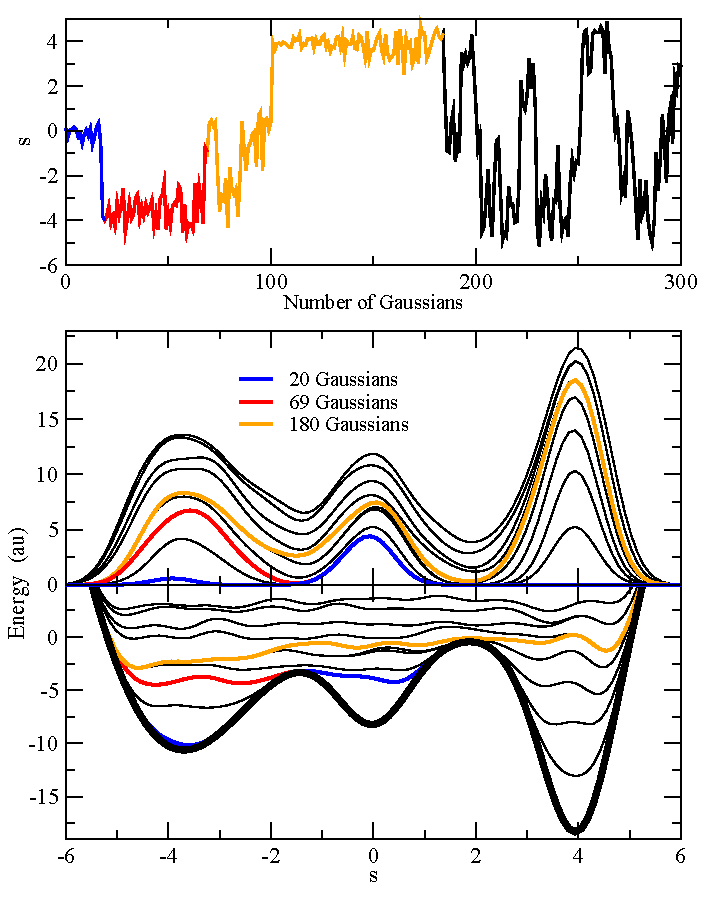
\includegraphics[width=0.55\textwidth]{./img/metadEs}
	\caption{Example of a time evolution of a metadynamics simulation. Top: time evolution of the \acs{CV} of a system evolved on the 3--minima \acs{FES} represented by the black thick line in the lower panel. Middle: time evolution of $w_M$, the history--dependent bias potential. Blue line: $w_M$ when the first minimum is filled and the system escapes to the second minimum; red line: $w_M$ when also the second minimum is filled; yellow line: when the entire profile is filled and the dynamics becomes diffusive on the whole energy landscape. Lower panel: time evolution of the sum of $w_M$ (same color scheme). Taken from \cite{MetadReview}.}
	\label{fig:metadEs}
\end{SCfigure}

Keeping in mind figure~(\ref{fig:metadEs}) a summary of the behavior of metadynamics and the validity of 
equation~\eqref{eq:metadfes} can be qualitatively understood in the limit of slow deposition. This means that 
$w_M(\vec s, t)$ varies slowly and the probability to observe $\vec s$ is approximately proportional to the 
Boltzmann factor $e^{-\beta(G(\vec s) - w_M(\vec s, t))}$. If the function in the exponential has some local 
minimum due to $G(\vec s)$, $\vec s$ will preferentially be localized in the neighborhood of this minimum and an 
increasing number of Gaussians have to be added until it is completely filled. When the minimum is filled the 
system reaches the condition $G(\vec s) \sim w_M(\vec s, t)$, the probability distribution would be approximately 
flat and we can say that the system becomes diffusive in the region explored by the simulation. Then, in this 
region, the placement of new Gaussians is no more affected by the difference between $G(\vec s)$ and 
$w_M(\vec s, t)$ and they are deposited randomly over the flat free energy profile. The \acp{FES} reconstructed 
after that point, as visible in figure~(\ref{fig:metadEs}), are affected by some corrugations, due to newly 
deposited Gaussians, of the order of $w$. From that point the metadynamics has reached the \textit{convergence} 
in the sampled region.

\paragraph{\textbf{convergence}} As just explained before, the convergence of the metadynamics in a specific 
region of the \acp{CV} space is reached when the system become diffusive in this region, i.e. when the \acp{CV} 
can assume all possible values compatible to the sampled region. This is a crucial point for the metadynamics 
method in order to obtain the best possible estimator of the \ac{FES}, in the sampled region. Clearly, in order 
to save computational time, if one want only to give the possibility to the system to escape from an energy 
minimum is not necessary to reach the convergence otherwise it is an important point. Unfortunately in most 
systems it is not trivial to identify precisely when the diffusive regime has been reached. In most cases a 
practical method to assess the convergence of metadynamics simulations is based on monitoring the free energy 
difference between two reference point: when the difference is approximately flat then the convergence should be 
reached.

\paragraph{\textbf{error estimation}} After convergence is reached the error on the \ac{FES} estimator is clearly 
dependent on the chosen parameters. The best way to estimate the statistical error introduced by the metadynamics 
is to perform several statistically independent metadynamics runs. The arithmetic average of all the 
history--dependent potentials taken at the same time, after the convergence is reached, is equal to the best 
estimate of the \ac{FES}. The statistical error of the \ac{FES} of a run can be considered as the standard 
deviation between the history--dependent potential $w_M(s,t)$ of that run and the averaged \ac{FES} 
$G(\vec s) \sim - \overline{w_M(\vec s,t)}$ and average it over the whole \acp{CV} space, as follow
\begin{equation*}
\overline{\epsilon}^2 = \frac{1}{\Omega_s} \int_{\Omega_s}  \overline{(w_M(\vec s,t) - \overline{w_M(\vec s,t)})^2}\ ds
\end{equation*}
where $\Omega_s$ is the whole \acp{CV} space. Laio \etal\, in \cite{MetadError}, by performing extensive 
numerical simulations of a Langevin stochastic system, have derived an approximate expression for the error 
estimator in function of the system and metadynamics parameters, as follow
\begin{equation*}
	\overline{\epsilon}^2 \propto \frac{LT}{D}\frac{w}{\tau} \delta s 
\end{equation*}
where $L$ is the size of the simulation box, $D$ is the system diffusion coefficient and $T$ is the system 
temperature. Since $\delta s$ is approximately fixed by the fluctuation of the \acp{CV} in a unbiased \ac{MD} run 
and/or by the granularity to be achieved in the \ac{FES} estimator, the error is dominated by the ratio $w/\tau$. 
Thus a fine tuning of the Gaussians height and deposition pace is often needed in order to minimize the 
statistical error. Despite this, it is commonly accepted to follow a procedure for the \ac{FES} and error 
estimators:
\begin{itemize}
	\item Several statistically independent metadynamics simulations are performed;
	\item After the convergence is reached for each run, the estimator of the \ac{FES} is the arithmetic average of the \ac{FES} obtained from equation~\eqref{eq:fes} for each simulations (each free energy profile appropriately normalized);
	\item The statistical error on the averaged \ac{FES} is performed considering its standard deviation. 
\end{itemize}
Alternatively one can perform a very long metadynamics run in which, for example, the system is diffusive for 
half simulation. Then one can chose as statistically independent history--dependent potentials some of them 
computed at different times in the diffusive region and follow the above procedure from the second point. Clearly 
one has to be careful about the decorrelation time between the chosen profiles, otherwise they are not 
statistically independent due the continuos nature of the metadynamics algorithm.

\paragraph{\textbf{performance optimization}} In general the computational overhead of adding metadynamics to an 
\ac{MD} simulation is usually not excessive, even if it depends on the implemented algorithms. However as the 
number of deposited Gaussians increases, in each \ac{MD} step a larger and larger number of exponential terms 
have to be computed and summed in order to calculate the derivative of the history--dependent potential, i.e. the 
forces due to the metadynamics. Thus if the Gaussians are big or frequently deposited or the system takes a lot 
of time to reach the convergence, the computational overhead scales as the number of the deposited Gaussians. 
This can clearly lead to a loss of performance as the simulation time increase. A simple solution is to implement 
a discrete mesh grid on the \acp{CV} space in which the history--dependent potential is spread and stored. When a 
new Gaussian is added the potential is updated in the whole grid. While, at each \ac{MD} step, in order to 
compute the derivative, the potential in a non--grid point is only estimated from an interpolation of some 
neighbor grid points, depending on the interpolation order. By this trick the computational overhead remains 
approximately constant as the simulation time increase.

\subsection{Umbrella sampling and metadynamics remarks}
Despite metadynamics is relatively recent while umbrella sampling is a well known and optimized method the former is steadily spread in the computational community against the latter. The most relevant reasons are its simplicity of implementation and the direct way to control efficiency and performance by changing the parameters of the Gaussians entering in the history--dependent potential. This gives to the metadynamics the possibility, with only one framework, to overcome different situations such as passing continuously from a fast and coarse exploration of the energy landscape to an accurate evaluation of the free energy profile, predict new stable configurations and structures, new reaction pathways, calculate free energy profiles and free energy differences.

In umbrella sampling the reconstruction of the free energy profile follow a predefined scheme designed for covering the chosen \acp{CV} space. In contract a well implemented metadynamics reconstruct efficiently the free energy profile. Starting from the current minimum and explore a larger and larger region of the accessible phase space dwelling on the low energy regions, which are statistically the most relevant, avoiding spend to much time in the irrelevant regions, the \ac{FES} is recursively reconstruct. Moreover which the advantage that each point in the \acp{CV} space is explored several times during the simulation. However a careful choice of the \acp{CV} is needed otherwise the history--dependent potential (and the reconstructed \ac{FES}) can evolves in an unpredictable manner.   

In a recent work by Davide Bochicchio \etal\, \cite{metaUSComparison} both methods for the \ac{FES} estimation included the error estimation, performance and accuracy are extensively compared with \ac{MD} simulations involving the transfer of a hydrophobic oligomers from water phase to hydrophobic core of a lipid membrane. The authors consider both at atomistic and \ac{CG} levels (\martini \ac{FF}). The authors found that, if the \acp{CV} are properly chosen and the parameters for the metadynamics are carefully tuned, the energy profiles reconstructed are reasonable identical between umbrella sampling and metadynamics, but the latter yields the same accuracy in a less time consuming simulation.  


%Manuale GROMACS 3.17.5 PP/PME ranks %Introduction to Molecular Dynamics

% !TEX root = ./../main.tex
\chapter{Empirical force field model}
\label{chap:EmpiricalFF}
As we have seen in the previous section \ac{MD} provides a variety of tools for solving the time evolution of a
$N$--particle system. Due to the possibility to capture different length and time scales \ac{MD} simulations can
be used to study a variety of systems, such as set of atoms, molecules or more complex systems such as proteins 
and macromolecular systems. Biomolecular simulations, especially when requiring the explicit treatment of 
solvent molecules, often deal with a very large number of particles $(10^4 < N < 10^6)$. As for the time scales, 
they can span a broad range depending on the process under study: hydrogen bond formation in organic molecules, 
for example, happens on the picosecond time scale; slow processes such as the diffusion of massive colloidal 
particles take place on time scales of milliseconds if not seconds.

% In each of these systems, depending on the \textit{interaction model} and its
% \textit{parametrization}, we will be able to describe crucial molecular--level processes, such as hydrogen bond
% formation in organic molecules, which happen on the picoseconds time scale; or study slow processes such as the
% diffusion of massive colloidal particles, taking place on time scales of milliseconds if not seconds. Considering
% soft or condensed mater, the most relevant for this thesis, the main processes of interest ranging from protein
% folding to glass transitions, from surface diffusion to ligand--receptor binding take place on longer time scales
% (several ns) and involve a larger number of atoms ($N \gg 10^4$).

The possibility to achieve the description of such a variety of systems by the same tool, \ac{MD}, relies on the 
existence of appropriate models of the interactions between atoms and molecules. In soft or condensed matter 
systems these interaction models always rely on the \textit{Born--Oppenheimer approximation}. It consists in 
separating the motion of the electrons by the motion of the atomic nuclei. This is done in order to integrate 
out the high frequency electrons' motions. Indeed, the explicit treatment of the electronic \ac{DOF} would 
limits the applicability of \ac{MD} to very small systems ($N$ of the order of $10^2$ atoms). In the following, 
when we speak about atoms or chemical moieties we refer to nuclei coordinates only without considering electrons 
at all.

%If, for some particular system, we want to know precisely the dynamics of the electrons we have to introduce quantum mechanical methods that are, even for a small number of particles ($N\sim 10^2$), very computationally time consuming. 

Hence, to describe the dynamics of a biomolecular system it is necessary to develop a \textit{classical model of 
the inter--atom interactions}. The set of functional forms of the interaction potentials between atoms and 
molecules and they parameterization are collected into the so called \textit{empirical \acf{FF}}. The meaning of 
\textit{empirical} is that most of the functional forms of the interaction potentials has no ``first principle'' 
justification: they are chosen as a compromise between accuracy and computational efficiency. For biomolecular 
applications two main classes of \acp{FF} exist: the \textit{atomistic} \acp{FF} in which basic
particles are atoms, and the \textit{\ac{CG}} \acp{FF} in which the basic particles represent atom groups or
small chemical moieties.

% Nevertheless atom or molecule interactions, such as bond formation, are mediated by the electron interactions.
% Thus, to describe the dynamics of such a system with a classical \ac{MD} tools and the Born--Oppenheimer
% approximation, it is necessary to develop an  Since forces are derived from the \ac{PEF}, a typical choice, when it is possible, for
% example with organic systems, is to model the inter--particle interactions by a set of pairwise addictive
% potentials that avoid any many--body calculations. Nevertheless for some systems this is impracticable, for
% example, for metal cores we need to consider the many--body calculations or an effective many--body potential
% that take into account the behavior of all metal atoms in the core. A typical solution is to use the many--body
% potential developed by Gupta (see \cite{Leach} for more details about metals treatment at \ac{MD} level).
%Further it is necessary to stress out that a \ac{FF} is a well defined single entity containing the simulation parameters, the functional models of the interactions and also its parameterizations (and the way to obtain it). All the parameters of a \ac{FF} are in harmony to each other thus changing some parameters without retesting whole \ac{FF} is not allowed because, maybe, one can destroy the whole \ac{FF}.

\paragraph{\textbf{\textacr{parameterization}}} In general the functional forms for potential interactions are
common to all particles in the system. The \ac{FF} is completed by a set of empirical parameters that
characterize the interaction between different types of particles, whether they are atoms or whole chemical
groups. Interaction parameters are empirical in the sense that they are assigned to reproduce a small set of
target properties on a small group of systems. These target properties can be derived from experimental
measurements or from finer--level calculations or simulations. Nowadays, atomistic and \ac{CG} biomolecular
\acp{FF} come as ``packages'' of parameters and functional forms appropriate for the description of a large
variety of chemical compounds in the liquid and solid phases.

\paragraph{\textbf{\textacr{transferability}}} As described above the parameterization of a \ac{FF} involves a
small set of test systems for which some set of target properties are reproduced. An important characteristic of 
a \ac{FF} is its \textit{transferability} that means the ability of the model to describe situations that
differ from those used at the parameterization stage. For example, a \ac{FF} parameterized to reproduce the 
physical properties of liquid water in standard ambient conditions should also reproduce other properties such 
as water melting point, liquid--vapor surface tension, and so on. This is the most challenging aspect of model 
development, and it relies on a very accurate choice of the target properties used during the parameterization 
stage.\\\medskip

In this chapter we will describe atomistic and \ac{CG} \acp{FF} in detail. We will describe the most common 
functional forms for modeling the inter--particle interactions and how to treat them in an \ac{MD} simulation. 
In the last part of the chapter we will focus on the main \ac{CG} \ac{FF} used in this thesis work: the 
\martini{} \ac{FF} developed by Marrink \etal{} in \cite{Martini}.

\section{Inter--particle interactions}
For biomolecular applications the inter--particle interaction potentials are divided into two main classes: the
\textit{bonded interactions} involving particles within the same molecules and the \textit{non--bonded
interactions} engaging all particles in the system and which usually represent the Van der Waals and the
electrostatic interactions. In the following the most common and general functional form for the \ac{PEF} is
described. In general the \ac{PEF} can be always splitted in bonded and non--bonded contributions:
\begin{equation*}
	U(\vec r) = U_{\text{b}}(\vec r) + U_\text{nb}(\vec r)
	\label{eq:FFPEF}
\end{equation*}

The bonded contribution is generally described by the following terms
\begin{equation}
	\begin{aligned}
	U_{\text{b}}(\vec r) = &\frac{1}{2}\sum_{\text{bonds}} \frac{1}{2}k_i^b(l_i - l_{i0})^2\ + \frac{1}{2}\sum_{\text{angles}} k_i^a (\theta_i - \theta_{i0})^2 +\\
		 	& +\frac{1}{2}\sum_{\text{torsions}} V_n(1+\cos (n\omega - \gamma))
	\end{aligned}
	\label{eq:bondPEF}
\end{equation}
the first two terms are harmonic potentials which model respectively the energy contribution due to the deviation
from reference bond length $l_{i0}$ and a bond angle $\theta_{i0}$. $k_{bi}$ and $k_{ia}$ are the bond and angle
elastic constants. The bond contribution involves a set of two adjacent particles while the angle contribution a 
set of three consecutive particles in the same molecule. The last term in equation~\eqref{eq:bondPEF} concerns 
the energy contribution due to the bond torsional change. It involves four consecutive particles in the same 
molecule and mimic the energy barrier needed to torsion the bond along the bond axis. $\omega$ is the torsional 
angle, $\gamma$ is a phase factor, $V_n$ qualitatively describes the energy barrier for each $n$--th components 
and $n$ is defined as the number of minima for each components.

The non--bonded contribution is described by the following terms
\begin{equation}
	U_\text{nb}(\vec r) = \sum_{i=1}^N \sum_{j>i} \left ( {4\epsilon_{ij} \left ( \left ( \frac{\sigma_{ij}}{r_{ij}} \right )^{12} - \left ( \frac{\sigma_{ij}}{r_{ij}} \right )^6 \right )  + \frac{q_iq_j}{4\pi\varepsilon_0 r_{ij}}} \right )
	\label{eq:nonbonPEF}
\end{equation}
The first term is the energy contribution due to the Van der Waals interactions modeled as a Lennard--Jones
$12-6$ potential, fully characterized by the constants $\sigma_{ij}$ and $\epsilon_{ij}$ assigned to each
pair of particles. The last term is the electrostatic energy contribution described by the particle charge $q$. 
The non--bonded interactions involve obviously all particles in the system, but for particles belonging to same
molecule they are usually computed only if they are separated by at least three bonds, i.e. if their 
interactions are not described by bonded terms. The various contributions described above are schematically 
represented in figure~(\ref{fig:FFInteraction}).
\begin{figure}[!ht]
	\centering
	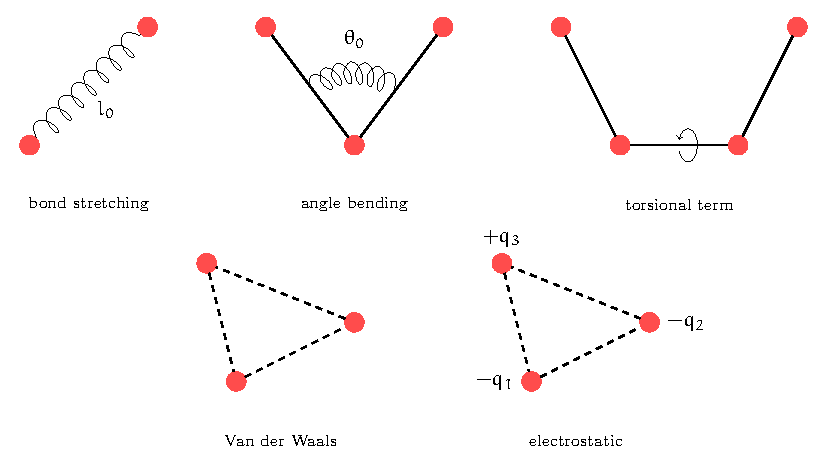
\includegraphics[width=0.8\textwidth]{./img/interPartInt/interPartInt}
	\caption{Schematic representation of the common inter--atom interactions for biomolecular applications: bond stretching, angle bending, torsional term, Van der Waals and electrostatic interactions.}%
	\label{fig:FFInteraction}
\end{figure}

\subsection{Cut--off, shift and switch methods}
The bonded interactions, as we can see in equation~\eqref{eq:bondPEF}, have a \textit{fixed range} of action, 
meaning that they depend, for example, on the equilibrium bond length that is fixed. Moreover, usually in 
standard \ac{MD} simulations bond breaking is not taken into account. The non--bonded interactions, instead, 
depend on the inter--particles distance $r_{ij}$ and decay to zero as a power of $r_{ij}^{-d}$. Depending on the 
power order $d$ compared to the dimensionality $s$ of the system they are split into \textit{short range} if 
$d>s$ and \textit{long range} interactions if $1 \le d < s$. For example, as we shall see later, the 
Lennard--Jones $12-6$ potential decays to zero as $r^{-6}$ then it is a short range interaction, while the 
electrostatic is a long range interaction since it decays to zero as $r$.

As we have mentioned in section~\ref{sec:neighbor} the calculations of non--bonded interaction energy
contributions is one of the most time consuming part of an \ac{MD} simulation. Even if we use a simple pairwise
additive potential their calculation scale as $\sim N^2$. Thus, especially for short range interactions, various
methods were developed in order to speed--up the simulation. The \textit{cut--off} method is the most used to
treat the short range interactions and, in some cases, even the long range ones. Taking one particle into
account, the general idea is to evaluate the non--bonded interactions with all other particles that are closer to
the first for a distance $r_c$, called \textit{cut--off} radius, otherwise the interactions is set to $0$. This
means that the new potential is of the form
\begin{equation*}
v^*(r) = \left \{
	\begin{aligned}
&v(r) & \quad & r \le r_c \\
&0    & \quad & r >   r_c
	\end{aligned} \right .
\end{equation*}

This generates a discontinuity in the potential and in its first derivatives, i.e. in the forces: this is bad for
energy conservation. A trick for solving the discontinuity of the potential and to improve the energy
conservation is to apply also a \textit{shift} of the potential value at $r_c$ so that $v^*(r_c) = 0$. Adding a
constant will not affect the force calculations. The potential becomes
\begin{equation*}
v^*(r) = \left \{
	\begin{aligned}
&v(r) - v(r_c) & \quad & r \le r_c \\
&0    & \quad  & r >   r_c
	\end{aligned} \right .
\end{equation*}

Moreover, to solve the discontinuity of the forces, that can cause some instability, a simple possibility is to
consider a linear term proportional to the first derivative of the potential, such as
\begin{equation*}
v^*(r) = \left \{
	\begin{aligned}
&v(r) - v(r_c) - \left . \frac{dv(r)}{dr}\right |_{r_c}\ (r - r_c) & \quad & r \le r_c \\
&0    & \quad  & r >   r_c
	\end{aligned} \right .
\end{equation*}
The shift methods can make the potential quite different from the original one. So this have to be properly taken
into account in order to retrieve the correct thermodynamic properties.

Another powerful method to solve the discontinuity problem of the potential and forces is the \textit{switch}
method. The general idea is to consider two cut--off radii  $r_{c1}$ and $r_{c2}$. If $r \le r_{c1}$ the original
form is used; while if $r > r_{c2}$ the potential is set to zero. If $r_{c1} < r \le r_{c2}$ a \textit{switching
function} is considered in order to \textit{smoothly} switch the potential to zero.

It is important to stress out that even the method used to treat the interactions, as the cut--off radii and
eventually the switching function, are part of the simulation parameters that are, in turn, part of the \ac{FF}.
So they are interdependent with the model parameterization, and should never be changed without retesting the
target properties of the parameterization.

\section{Van der Waals interactions}
Van der Waals forces are a set of interactions that can be ascribed to quantum dynamic effects. In general they
are described by a sum of a repulsive and an attracting term. The former effectually takes into account the Pauli
exclusion principle between electron clouds; the latter is related to the dipole--dipole interactions (Keesom
forces), dipole--induced dipole interactions (Debye forces), induced dipole--induced dipole interactions, London
dispersion forces, hydrogen bonding and entropy effects, that involves both polar and non--polar atoms.

The usual way to treat the Van der Waals interactions is to use a pairwise Lennard--Jones potential. The most
common exponents for the attractive and repulsive contributions are $6$ and $12$, respectively. The former 
exponent has physical meaning, as it describe the attractive term of dipole--dipole interactions. The latter, 
instead, is chosen for computational reasons: giving the $r^{-6}$ term it is efficient to calculate $r^{-12}$ as 
the square of $r^{-6}$. The general form for a $12-6$ Lennard--Jones potential is the following
\begin{equation}
	v(r) = 4\epsilon\left ( \left ( \frac{\sigma}{r}\right )^{12}  - \left ( \frac{\sigma}{r} \right )^6 \right ) = \frac{C_{12}}{r^{12}} - \frac{C_{6}}{r^{6}}
	\label{eq:lj126}
\end{equation}
where $C_{12} = 4\epsilon\sigma^{12}$, $C_{6} = 4\epsilon\sigma^{6}$ and $r$ is the pairwise particles distance.
$\epsilon$ is related to the absolute value of minimum while $\sigma$ is related to the position of the minimum
of the potential: $r_{\text{min}} = 2^{\nicefrac{1}{6}}\sigma$, often referred to by Van der Waals radius. These
constants are assigned to each particle pair. In figure~(\ref{fig:LG12511}) a plot of the 
function~\eqref{eq:lj126} with $\epsilon = \sigma = 1$ is shown.
\begin{figure}[!ht]
\centering
	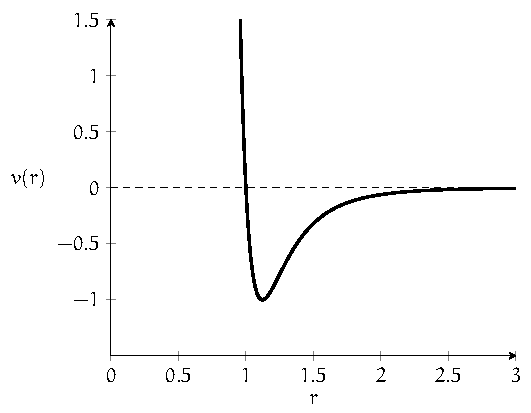
\includegraphics[width=0.6\textwidth]{./img/LJ126/LJ126}
	\caption{Plot of a Lennard--Jones interaction potential with $\epsilon = \sigma = 1$.}
	\label{fig:LG12511}
\end{figure}

The simplest and computationally most efficient way to treat a Lennard--Jones function, and in general all the
short range interactions, is to use the cut--off method together with the shift or switch methods in order to
obtain a continuous potential and/or a continuous forces. As we can see from figure~(\ref{fig:LG12511}) the
Lennard--Jones potential vanishes rapidly with distance: at $r \sim 2\sigma$ its value is less then $1\%$ of the
value in $r \sim \sigma$. A good choice for the cut--off is then of the order of $r_c \sim 2\sigma \div 3\sigma$.

\section{Electrostatic interactions}
\label{sec:electrostaticInt}
Despite the long range characteristic of the electrostatic interaction, for computational efficiency reason, most
of the \acp{FF} for biomolecular applications treat them in the same way as a short range interaction by a
cut--off method\footnote{In general, for computational reason, a common choice is to consider the same cut--off
for Van der Waals and electrostatic interactions.}. Of course this is an approximation and can lead to serious
issues in those properties or systems that strongly depend on the electrostatic interactions. As an example we
report some situations in which the use of the short--range electrostatics can lead to artifacts: they are
related to the development of a good polar solvent model (a good treatment of the electrostatic properties of
water is really important for biological applications), as well as to the study of the interactions of charged
particles with polar solvents, transport processes of charged moieties, calculations of the electrostatic
potential inside macromolecules and so on.

If we consider only the simulation box the electrostatic energy contribution is
\begin{equation}
	U = \frac{1}{2}\sum_{i=1}^N\sum_{j\ne i}^N\frac{1}{4\pi\varepsilon_0}\frac{q_iq_j}{r_{ij}}
	\label{eq:electrostatic}
\end{equation}
where $q_i$, $q_j$ and $r_{ij}$ are the charges and the distance, respectively, between particles $i$ and $j$.
But we need also all image boxes. Let us suppose, for simplicity, a cubic box of size $L$. We can
define a tern of integer numbers $(n_x,\ n_y,\ n_z)$, $n_i=0,1,2,\cdots$ so that the position of all other image
boxes, with respect to the central simulation box, is $\vec n = L (n_x,\ n_y,\ n_z)$. Then the energy
contribution becomes
\begin{equation}
	U = \frac{1}{2}\ \sideset{}{'}\sum_{n_x,n_y,n_z}^{+\infty}\ \sum_{i=1}^N\sum_{j=1}^N\frac{1}{4\pi\varepsilon_0}\frac{q_iq_j}{\|\vec r_i - \vec r_j + \vec n \|}
	\label{eq:electrostaticImage}
\end{equation}
where the prime indicates that for $\vec n = 0$, i.e. the energy contribution of the simulation box, we need to
exclude the self interaction term: in the inner sum it must be $j \ne i$.

As described above, a cut--off method is a good easy way to solve equation~\eqref{eq:electrostaticImage} and 
sometimes it produces sufficiently good results. The main problem is that the summation in 
equation~\eqref{eq:electrostaticImage} is \textit{conditionally convergent}
\footnote{A conditionally convergent series contains both positive and negative terms such that the positive or 
negative term alone form both a divergent series. The sum of a conditionally convergent series depends on the 
order in which the positive and negative terms are considered.} 
and converges extremely slowly so that it would need so many terms to converge that its computational cost would 
be too high, especially for large systems (of the order of $N \gg 10^4$). However, the increasing of computer 
power has led to develop more rigorous methods to solve equation~\eqref{eq:electrostaticImage}, even for very 
large systems. The most important methods developed to solve this problem are based on the \ac{ESM}. We shall 
describe those used in this thesis work: the \ac{ESM} itself and the \ac{PME} method. For a more complete 
discussion about the advanced methods developed to treat the electrostatic interaction, for biological 
applications, the reader is addressed to the review by Cisneros \etal{} \cite{Cisneros}.

\subsection{Ewald summation method} %Molecular Modelling, 334
The \acf{ESM} is the first method introduced by Ewald for a correct treatment of the electrostatic energy
contribution in an ionic crystal. The basic idea is to split the summation in equation~
\eqref{eq:electrostaticImage} in two series both rapidly convergent. The method is based on the following 
identity
\begin{equation}
	\frac{1}{r} = \frac{f(r)}{r} + \frac{1 - f(r)}{r}
	\label{eq:ewaldTrick}
\end{equation}
the trick is to choose a function $f(r)$ that will deal with the rapid variation of the $1/r$ term for small $r$
and the slow decay at long $r$; in that case the two series can rapidly converge.
\begin{figure}[!ht]
	\centering
	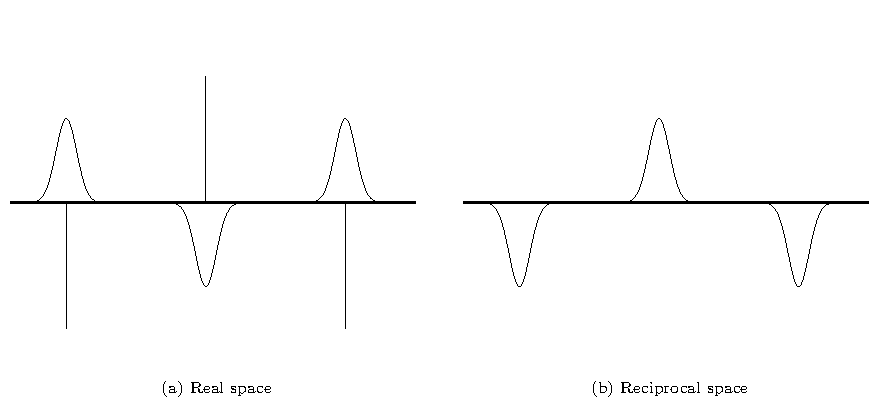
\includegraphics[width=0.8\textwidth]{./img/EwaldSum/EwaldSum}
	\caption{Schematic illustration of the \acs{ESM} charge distribution: in (a) point charges (represented by vertical lines) and the neutralizing Gaussian charge distribution; in (b) the counteracting Gaussian distribution.}%
	\label{fig:ewald}
\end{figure}

The \ac{ESM} for electrostatic interaction works, as illustrated in figure~(\ref{fig:ewald}), considering each
point--like charge in the system surrounded by a neutralizing charge distribution of equal magnitude but opposite
sign that decays rapidly to zero. Simplifying the notation for a one dimensional system, the simplest functional
form is a Gaussian distribution centered in the position $r_i$ of the point--like charge $q_i$, of the form
\begin{equation}
	\rho_i(r) = \frac{q_i\alpha^3}{\pi^{3/2}}e^{-\alpha^2 (r - r_i)^2}
\end{equation}
that obeys the relation
\begin{equation*}
	\frac{q_i\alpha^3}{\pi^{3/2}}\int_{r_i-\epsilon}^{r_i+\epsilon}e^{-\alpha^2 (r - r_i)^2}\ dr \simeq q_i
\end{equation*}
where $(r_i-\epsilon; r_i+\epsilon)$ is a small interval around $r_i$. The energy contribution due to this set
up, the point--like charge \textit{and} the gaussian charge distribution, is given by
\begin{equation}
	U_r = \frac{1}{2}\sum_{i=1}^N\sum_{j=1}^N\ \sideset{}{'}\sum_{n_x,n_y,n_z}\ \frac{q_iq_j}{4 \pi \varepsilon_0} \frac{\erfc{(\alpha \| \vec r_i - \vec r_j + \vec n \|)}}{\| \vec r_i - \vec r_j + \vec n \|}
	\label{eq:ewaldReal}
\end{equation}
where the prime indicate that for $\vec n = 0$ must be $i\ne j$, $\erfc{(x)} = 1-\erf{(x)}$ is the complementary
error function and $\erf{(x)}$ is the error function. They are given by
\begin{equation}
	\erfc{(x)} = \frac{2}{\sqrt{\pi}}\int_{x}^{+\infty} e^{-t^2}\ dt, \qquad \erf{(x)} = \frac{2}{\sqrt{\pi}}\int_{0}^{x} e^{-t^2}\ dt
	\label{eq:erf}
\end{equation}

The point is that the summation involving the complementary error function in equation~\eqref{eq:ewaldReal} is
rapidly convergent and it needs very few terms so that a cut--off method can be safely used. The rate of
convergence depends on the $\alpha$ parameter: the bigger is $\alpha$, the more rapidly the series converges and
the shorter the cut--off radius can be. Thus the \ac{ESM} use the $\erfc{(r)}$ as $f(r)$ function in
equation~\eqref{eq:ewaldTrick}. Of course since we added a non physical neutralizing charge in the system, in
order to restore the real charge distribution, we must consider another distribution, called counteracting charge
distribution, of equal magnitude but opposite sign. Considering the identity in equation~\eqref{eq:ewaldTrick}
this lead to an energy contribution $U_f$ of the form $(1-f(r))/r$. But using the relation between \erfc{} and 
\erf{} functions, it becomes of the form $\erf{(r)}/r$. Another important trick is to compute $U_r$ in the 
\textit{real space} while $U_f$ in the \textit{reciprocal space}, thus considering its Fourier transform. This 
energy contribution is given by 
\begin{equation}
	U_f = \frac{1}{2}\sum_{i=1}^N\sum_{j=1}^N\ \sum_{k_x,k_y,k_z}\ \frac{1}{4\pi\varepsilon_0}\frac{4\pi}{L^3k^2}e^{-k^2/(4\alpha^2)}e^{\mathsf{i}{\vec k \cdot (\vec r_i - \vec r_j)}}
	\label{eq:ewaldReciprocal}
\end{equation}
where $\vec k = 2\pi\vec n/L$ are the reciprocal lattice vectors. Even $U_f$ converges rapidly as $U_r$ in
equation~\eqref{eq:ewaldReal}; then a cut--off method can be safely used. Nevertheless, opposite to $U_r$, the
smaller is $\alpha$, the shorter the cut--off can be. Clearly a proper \textit{balance} between the real and
reciprocal space summation is needed.

Since in equation~\eqref{eq:ewaldReal} even the self interaction with each Gaussian is included we need to add
another item for cancel it out; this is done by the self--term
\begin{equation}
	U_\text{self} = -\frac{\alpha}{\sqrt{\pi}}\sum_{i=1}^N\frac{q_i}{4\pi\varepsilon_0}
	\label{eq:EwaldselfTerm}
\end{equation}

Summarizing, the energy contribution of the electrostatic interactions by the \ac{ESM} is computed summing
equations~\eqref{eq:ewaldReal},\eqref{eq:ewaldReciprocal} and~\eqref{eq:EwaldselfTerm} to obtain
\begin{equation}
	\begin{aligned}
		U =&\quad\frac{1}{2}\sum_{i=1}^N\sum_{j=1}^N\ \sideset{}{'}\sum_{n_x,n_y,n_z}\ \frac{q_iq_j}{4 \pi \varepsilon_0} \frac{\erfc{(\alpha \| \vec r_i - \vec r_j + \vec n \|)}}{\| \vec r_i - \vec r_j + \vec n \|}\ + \\
		 &+ \frac{1}{2}\sum_{i=1}^N\sum_{j=1}^N\ \sum_{k_x,k_y,k_z}\  \frac{1}{4\pi\varepsilon_0}\frac{4\pi}{L^3k^2}e^{-k^2/(4\alpha^2)}e^{\mathsf{i}{\vec k \cdot (\vec r_i - \vec r_j)}}\ + \\
		 &- \frac{\alpha}{\sqrt{\pi}}\sum_{i=1}^N\frac{q_i}{4\pi\varepsilon_0}
	\end{aligned}
	\label{eq:EwaldEnergy}
\end{equation}
The first line is the real space contribution while the second is the Fourier energy contribution. Since the
self--interaction term is constant it does not affect forces computation. The \ac{ESM} offers a well defined
method to properly treat electrostatic interactions, nevertheless it is quite expensive in term of computational
resources. If $\alpha$ and the cut--off are constant, then the computation scales as $\sim N^2$.

For biomolecular applications most \ac{MD} tools set an equal cut-off radius for both Van der Waals interaction
and the real part of the Ewald summation~\eqref{eq:EwaldEnergy} in order to achieve for both a scaling of the
order $\sim N$. However in this way the computation of the reciprocal part in the Ewald
summation~\eqref{eq:EwaldEnergy} will be very inefficient as it scales as $\sim N^2$. In order to increase the
efficiency of the calculation of the Fourier transform various advanced methods can be used. They are all based
on the use of the \ac{FFT} method. In this way the reciprocal part can scale as $\sim N\ln N$. Since \ac{FFT}
requires discretized quantities, the idea of such methods, called \textit{particle mesh}, is to consider the
charge density spread on a mesh grid and then evaluate the electrostatic potential via solving the Poisson's
equation\footnote{Given a charge distribution $\rho(\vec r)$ then the associated electrostatic potential
$\phi(\vec r)$ can be calculated solving the Poisson's equation 
$\displaystyle \nabla^2\phi(\vec r) = -\frac{1}{\varepsilon_0} \rho(\vec r)$. If a charge $q$ is at position 
$\vec r$ its electrostatic potential energy is given by $U = q\phi(\vec r)$.}
using fast Poisson solver together with the \ac{FFT} method. This can be done, for example, exploiting the
\ac{PBC} in order to discretize and make periodic the Poisson's equation. Such algorithms include the 
\textit{particle--particle particle--mesh} method, \textit{particle mesh Ewald} method, 
\textit{fast--Fourier Poisson} method and a recent methodology based on multi--scale mesh grid. The efficiency 
and accuracy of such mesh--based algorithms depend strongly on the way in which the charges are attributed to 
the mesh points (and it is also what makes the methods differ from each other). In the following we will 
describe the one used in this thesis work, the \acf{PME} method.

\subsection{Particle mesh Ewald method}
The \acf{PME} method developed by Darden \etal{} \cite{DardenPME} is based on the \ac{ESM} so the starting point
is equation~\eqref{eq:EwaldEnergy}. As described above, the first part of the Ewald summation is computed in the
real space together with the Van der Waals contribution using the same cut--off radius. The reciprocal part,
instead, is computed using \ac{FFT} method, in order to have a gain of performance. First, we need to
consider a grid mesh onto which the Gaussian counteracting charge distribution is spread. The basic idea, then,
is to calculate the electrostatic energy solving Poisson's equation through \ac{FFT} methods. The efficiency and
accuracy depend on the way the charges are distributed onto the grid. To do this a \textit{charge assignment
function}, $W(r)$ is introduced in such a way that, considering for simplicity a one dimensional system, the 
fraction of a charge at position $r$ assigned to a grid point at position $r_p$ is given by $W(r_p - r)$. Hence, 
if we have a charge density $\rho(r)$ then the charges at the grid point $r_p$ are given by
\begin{equation}
	q_M(r_p) = \int_0^L\ W(r_p - r) \rho (r)\ dr
	\label{eq:meshAssign}
\end{equation}
where $L$ is the box length and, if $h$ is the grid spacing, $M = L/h$ is the number of mesh point. In
figure~(\ref{fig:gidAssign}) the charge assignment is schematically represented.

The assignment function should have the following properties: it should be an even function and it should be
normalized in such a way that the sum of the fractional charges equals the total charge of the system. Moreover
the best accuracy is obtained with a dense grid in order to reduce as much as possible the discretization of the
charge density. However the computational cost increases as the number of grid points: a balance between
efficiency and accuracy is clearly needed.
\begin{SCfigure}
	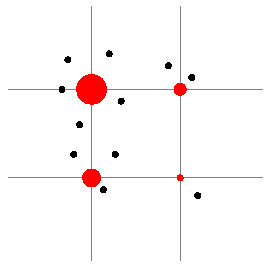
\includegraphics[width=0.35\textwidth]{./img/gridCharge/gridCharge}
	\caption{A schematic representation of the charge assignment. The black filled circles are a unit particle charge, while the red ones, are the charges assigned to grid points. The bigger is the circle, the more is the charge.}
	\label{fig:gidAssign}
\end{SCfigure}

A nice way to solve the problem of charge assignment is to shift the problem to the discretization of the Fourier
transform. This can be viewed as an interpolation problem. Consider the $e^{-\mathsf{i}\vec k\cdot \vec r_j}$
term in the Fourier transform of equation~\eqref{eq:ewaldReciprocal}. In general $\vec r_j$ does not correspond
to a mesh grid point, so this term is not part of a discrete Fourier transform. The idea, thus, is to interpolate
it in terms of the values of the complex exponential at the mesh points. Switching for simplicity to a one
dimensional system, if the mesh grid has $M = L/h$ points, a particle coordinate $r_j$ is located between mesh
points $[r_j/h]$ and $[r_j/h] + 1$ where $[\cdot]$ denotes the integer part; thus a $p$--order interpolation of
the exponential is of the form
\begin{equation*}
	e^{-\mathsf{i}kr_j} \simeq \sum_{i=1}^M W_{p}\left ( \frac{r_j}{h} - i \right ) e^{-\mathsf{i}khi}
\end{equation*}
where $W_{p}$ denotes the interpolation coefficient. A $p$--order interpolation means that only the $p$ mesh
points nearest to $r_j$ contribute to the sum. Assuming a point--like charge distribution the Fourier transform
of the charge density is therefore
\begin{equation*}
	\rho_k \simeq \sum_{i}e^{-\mathsf{i}khi} \sum_j\ q_iW_{p} \left ( \frac{r_j}{h} - i \right )
\end{equation*}
we can interpret the above expression as the discrete Fourier transform of the charge density
\begin{equation*}
	\rho(i) = \sum_j\ q_iW_{p} \left ( \frac{r_j}{h} - i \right )
\end{equation*}
but using equation~\eqref{eq:meshAssign}, it is nothing that the point--like charge distribution assigned to the
mesh point $i$ through the assignment function $W_{p}$.

We clearly see that the charge assignment problem is now shifted to the complex exponential interpolation. There
are two main methods to make the interpolation: the \textit{Lagrange interpolation method} and the \textit{Euler
SPLINE interpolation method}. The basic idea of the former is to use, as interpolating function, a polynomial
function of degree $ \le (n-1)$ where $n$ is the number of points to interpolate, that passes through all the $n$
points, and which is constructed with a summation over the \textit{Lagrange basis polynomials} as follows
\begin{equation*}
	P(x) = \sum_{i=1}^n y_i \prod_{\substack{k=1\\k\ne i}}^n \frac{x-x_k}{x_i - x_k}
\end{equation*}
where $(x_i;y_i)$ are the sets of points to interpolate. The main disadvantage of this method is that, even if
$P(x)$ is continuous everywhere, its derivative is not, thus it can lead to some instability in \ac{MD}
simulations.

The latter method, that is the most used in \ac{MD} tools, is based on the concept of \textit{SPLINE
interpolation}. Instead of using a unique interpolating function that passes through each point, the SPLINE
method uses a \textit{piecewise polynomial function}, called SPLINE, in which each piece is smoothly connected
and optimized to interpolate a subset of the points. The Euler SPLINE method use the \textit{exponential Euler
SPLINE} that is constructed with the basis of the Euler $n$--degree polynomials $A_n(x;\lambda)$ generated by the
following equation
\begin{equation*}
	\frac{\lambda - 1}{\lambda - e^z}e^{xz} = \sum_{n=0}^{+\infty} \frac{A_n(x;\lambda)}{n!}z^n
\end{equation*}
where $\lambda$ is a complex parameter and $z$ is a complex variable. The main properties of such SPLINE is that,
it is $n-1$ times analytic, continuously differentiable and then can solve the instability problem of the
Lagrange interpolation method. In literature the Euler SPLINE method is referred to as \textit{smooth} \ac{PME}
and the reader is addressed to the article by Essmann \etal{} \cite{EssmannSPME} for more technical details about
the interpolation procedure.

Summarizing, the \ac{PME} method is implemented with the following scheme
\begin{itemize}
	\item By the interpolation of the complex exponential in the Fourier transform of the Ewald summation, the
		  Gaussian counteracting charge distribution are spread onto the mesh grid;%
	\item Poisson's equation for the discretized charges are solved through the \ac{FFT} methods;
	\item The $U_f$ energy contribution is obtained considering the inverse Fourier transform;
	\item Electrostatic forces are computed and assigned to the charged system particles.
\end{itemize}

The main advantages of the \ac{PME} algorithm are that the potential energy and forces are smooth functions of
the particles positions. The method offers a good energy conservation and offers a good balance between accuracy
and computational efficiency since it scales as $\sim N\ln N$. Moreover, despite we have described \ac{ESM} and
\ac{PME} applied to the electrostatic interaction, they can be used, with some changes, with all long range
interactions and in general to all energy contributions that decay as $r^{-d}$, for example, even with the Van
der Waals energy contribution.

The general workflow shown in figure~(\ref{fig:MDscheme}) can be updated adding the calculation of the bonded and 
the non--bonded interactions and the \ac{PME} contribution. In figure~(\ref{fig:PPCore}) a summary of the new 
workflow is shown.
\begin{figure}[ht!]
	\center
	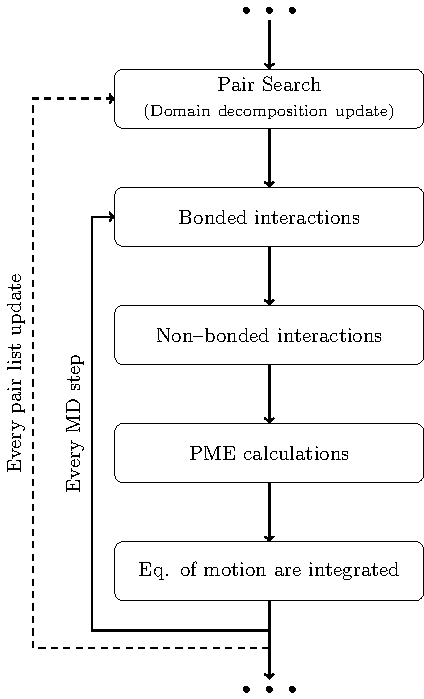
\includegraphics[width=0.5\textwidth]{./img/Schemi/PPCores}
	\caption{Schematic workflow of the particle interaction calculations inside an \acs{MD} simulation.}
	\label{fig:PPCore}
\end{figure}

\subsection{Charge representation}
\label{sec:chargeRep}
Even if some methods, such as the \ac{PME} one, have been developed to speed up the computation of electrostatic
energy contribution one of the main problems of \acp{FF} for biomolecular applications remains the \textit{charge
representation}: the way in which the charges of atoms or molecules are assigned to the system particles. The
problem arises from the necessity to represent the electron clouds and the interactions that generate.
Nevertheless this is crucial for a better description of most electrostatic phenomena such as polarizability of
molecules and polar solvent, solvation shell of charged ions, protein--ligand interactions, ion transport through
polar and non--polar medium, self assembly processes and so on.

The most common solution is the \textit{atom--centered ``partial charge'' approximation} in which the full charge
density of the molecule is replaced by fractional point--like charges assigned to each atom of the molecule.
Traditionally most non--polarizable \acp{FF} (as those we will use in this thesis work) assign to each atom of a
molecule a fixed partial--charge. The most used procedure for extracting partial--charges from molecular wave
functions is based on fitting atomic charges with the molecular electrostatic potential, computed with \textit{ab
initio} calculation such as \textit{density functional theory}. The fitting procedure consists in minimizing the
deviation between the electrostatic potential produced by the assigned charges and the molecular electrostatic
potential. Such representation is believed to be an important source of error in the electrostatics treatment.
Moreover with fixed charge assignment it is impossible to take into account those phenomena that involve a
transfer of charge inside the molecule, as polarization effect. The use of off--centered charges and/or higher
order atomic multipoles can significantly improve the treatment of electrostatics but of course it is necessary a
good balance between accuracy and performances since the electrostatic problem can rapidly drive to a loss of
computational efficiency.

\subsection{Polarization}
\label{sec:polarization}
Polarization refers to the redistribution of the electron charge density of a molecule in presence of an external
electric field, generated, for example, by charged ions or by another molecule. Polarization is responsible to
non--additive attractive inter-- or intra--molecular interactions which have many--body characteristics. These
effects have been recognized to have an important role in many biological interactions in which different
compounds are present. An increasing number of studies show that the lack of these effects can lead to serious
limitations, particularly, for systems that involve different environments such us water and proteins or water
and lipids. In \ac{MD} simulations polarization effects are included using either \textit{implicit} or
\textit{explicit} methods.

The implicit method completely avoids the many--body calculations by including a mean polarization effect in the
functional form of the interaction potential. The general idea is to surround all the simulation box by a
transparent medium with a relative dielectric constant $\varepsilon_r$. In this way the polarization effect is
taken into account considering a mean field theory and solving the Poisson's equation to determine the
electrostatic potential due to system charges by the substitution
$\varepsilon_0\rightarrow\varepsilon_0\varepsilon_r$. Since it avoids many--body calculations, this method gives
an incomparable gain in performances but it must be carefully used. The main disadvantage is that the mean
polarization effect is added to all system particles and this wash out all the details about a possible
polarization effect in a molecule. Moreover the electrostatic interaction between charged particles is affected
by the mean field effect. This produce a correct electrostatic interaction for particles inside the same solvent
for which the implicit medium is parameterized. Otherwise, if the simulation box is composed by different
chemical environments such as a polar and non--polar compounds, using the same dielectric constant would lead to
badly calculate the electrostatic interactions for particles in the non--polar environment. Thus, this method can
be safely used when our system is composed principally by one kind of solvent, for example water.

The way to correct the above behavior is to use an explicit method. As the name suggests, the polarization effect
is taken into account for every molecule in the system by an its proper model included in the \ac{FF}. The
general idea is to add some more internal \ac{DOF} to a molecule or atom to take into account the movement of
charges and/or split the point--like charge assigned, for example, to a chemical group, to a partial-charge
assigned to each particles of the chemical group itself. This can be done for every molecule or atom in the
system and thus it is the optimum to better describe systems with different chemical environments. Obviously this
method is more time consuming compared to the first.

%\subsection{Atomistic model}
\section{Coarse--Grained model}
\label{sec:CGModel}
As we have introduced at the beginning of this section, for biomolecular applications two main classes of
classical \acp{FF} exist: atomistic \acp{FF} and \ac{CG} \acp{FF}. Since the atomistic model takes into account
all the atoms in a molecule it is obviously the most realist and accurate \ac{FF}. Nevertheless the large number
of \ac{DOF} of atomistic \acp{FF} leads to a loss of computational performance. Moreover, basically, the
atomistic \acp{FF} are efficient until the physical properties can be properly sampled on a time scale of 
hundred of nanoseconds over a length scale of a few nanometers. As the time and length scales increase more and 
more time is needed to carry out a complete simulation. Unfortunately many biological processes involving lipid 
membranes and other organic molecules, including synthetic compounds, take place on much longer time (of the 
order of microseconds nor milliseconds) and length scales (of the order of tens nanometers).

One possible solution is to \textit{integrate out} some \ac{DOF}, preserving those that are relevant for the
problem in exam: this procedure is called \textit{coarse--graining}. The basic units of \ac{CG} \acp{FF} are
called \textit{beads}, each representing a group of atoms or a well defined chemical moiety. The size of the
group of atoms that is represented by a single bead determines the degree of coarsening of the \ac{FF}. Even in
this case, all the general features described above, apply: functional forms need to be chosen and their
parameterization need to be adjusted so as to reproduce the desired target properties. In figure~(\ref{fig:CGLevels}) different levels of coarse--graining are showed.
\begin{figure}[h!t]
	\centering
	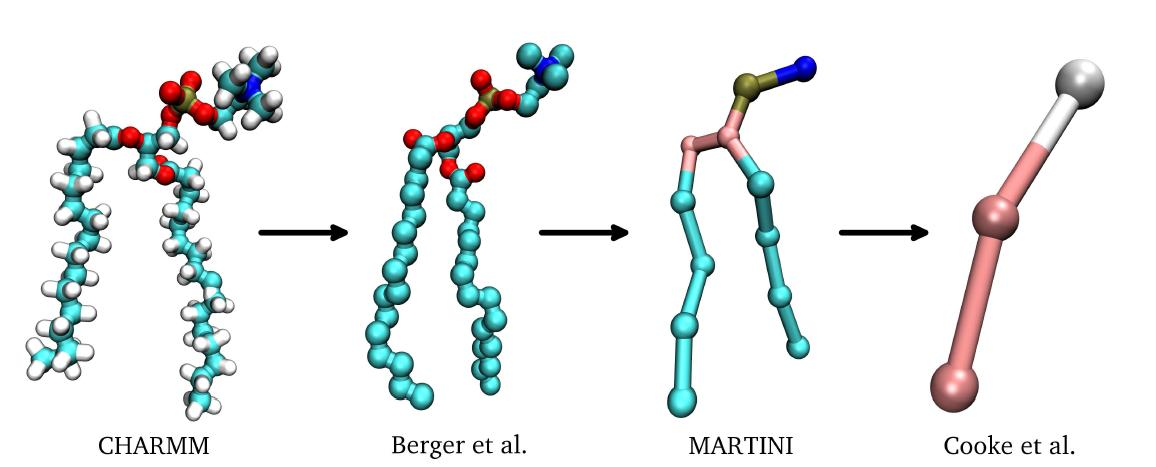
\includegraphics[width=0.7\textwidth]{./img/CGMapping}
	\caption{Different levels of the coarse--graining of a phospholipid. From left to right increasing levels of coarse--graining. Taken from \cite{CoarseGrainingMapping}.}%
	\label{fig:CGLevels}
\end{figure}

The first step in the development of a \ac{CG} model is the \textit{mapping} procedure. This establishes a link
between the atomistic model and the \ac{CG} one. There is not a unique or correct procedure to perform the
mapping because it depends on the desired coarse--graining level, on the time and length scales that one wants to
correctly sample and on the properties one wants to reproduce. For biological applications \ac{CG} \acp{FF} are
often designed to reproduce specific thermodynamic properties such as surface tension, free energy of
partitioning, free energy of hydration and so on. \ac{CG} \acp{FF} employed in the material sciences (e.g.
polymer science) often use as a target the material structural properties.

In general a \ac{CG} \ac{FF} is more computationally efficient than an atomistic one for the following reasons
\begin{itemize}
	\item the \ac{DOF} of the system are reduced due to the \ac{CG} procedure with the consequence that a smaller number of interactions and forces has to be computed;%
	\item bead--bead interactions, which result from the removal of finer structural details, are softer than atom--atom interactions;%
	\item vibrational modes are slower, and their sampling can be achieved using larger \ac{MD} time steps than in atomistic simulations;%
	\item softer interactions imply a smoother \ac{PEF} which leads to faster diffusion.
\end{itemize}

\section{MARTINI: a Coarse--Grained Force--Field}
\label{sec:martini}
\martini{} is a \ac{CG} \ac{FF} developed by Marrink \etal{} \cite{Martini} for organic solvents and lipids and
then extended to proteins \cite{MartiniProtein}, carbohydrates \cite{MartiniCarbo} and a broad class of polymers
\cite{MartiniPolymers}. \martini{} is based on a chemical building block approach. Such \martini{} blocks or beads
represent small chemical moieties and they are extensively calibrated in order to construct a large variety of
organic molecules. As we shall see in section~\ref{sec:martiniParam}, the \ac{FF} is based on accurately
reproducing the interaction between polar and non--polar chemical compounds. The main target property is intact
the \textit{partitioning free energy} between water and a large number of organic solvents, i.e. the free energy
of transfer of chemical moieties from polar and non--polar solvents.

\subsection{Mapping}
The mapping of the \martini{} beads is based on a four--to--one scheme that groups four heavy atoms like C, S, O
and so on, plus their associated hydrogen atoms, into a single interaction site. Consistently four water
molecules are modeled with one \martini{} bead. An example of the mapping procedure including both atomistic and
\ac{CG} descriptions is shown in figure~(\ref{fig:martiniMapping}).
\begin{figure}[!ht]
	\centering
	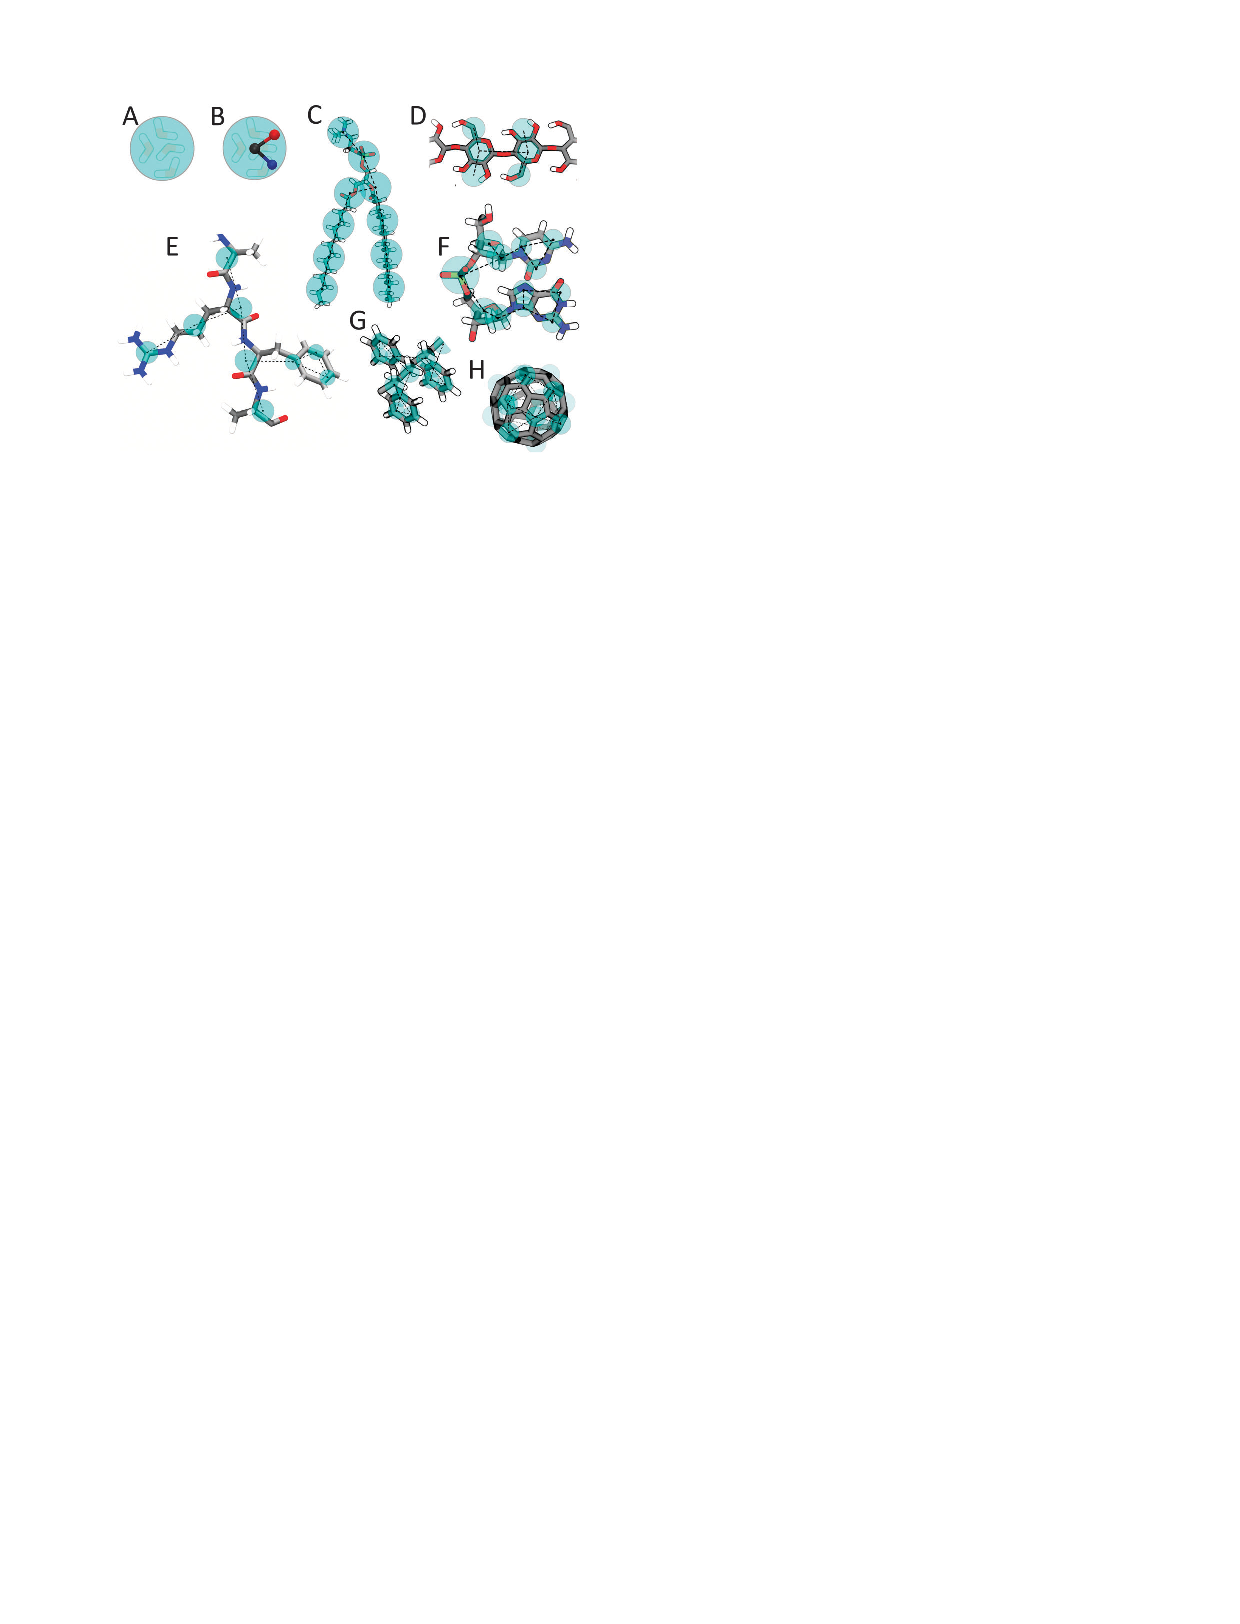
\includegraphics[width=0.5\textwidth]{img/martiniMapping}
	\caption{\martini{} mapping and atomistic structures compares of some molecules: (A) Standard water bead, (B) polarizable water bead, (C) \acs{DMPC} lipid, (D) Polysaccharide fragment, (E) Peptide, (F) DNA fragment, (G) Polystyrene fragment and (H) Fullerene molecule. In all cases \martini{} \acs{CG} beads are shown as cyan transparent beads overlaying the atomistic structure. Taken from \cite{MartiniReview}.}%
	\label{fig:martiniMapping}
\end{figure}

There are four main bead types: polar (P), non--polar (N), apolar (C) and charged (Q). Each bead type has a
number of subtypes to take into account a more accurate representation of the chemical nature of the moieties due
to the underlying specific atomistic structure. These subtypes are distinguished by the hydrogen bonding
capabilities: donor (d), acceptor (a), both donor and acceptor (da) and none ($0$) and/or by their degree of
polarity: lowest polarity ($1$), $\dots$, highest polarity ($5$).

\begin{SCtable}\footnotesize
	\begin{tabular}{lc}
		\toprule
		Level  & $\epsilon$\,[kJ/mol] \\ \midrule
		O	   & $5.6$	 \\ \midrule
		I      & $5.0$	 \\ \midrule
		II	   & $4.5$	 \\ \midrule
		III	   & $4.0$	 \\ \midrule
		IV	   & $3.5$	 \\ \midrule
		V	   & $3.1$	 \\ \midrule
		VI	   & $2.7$	 \\ \midrule
		VII	   & $2.3$	 \\ \midrule
		VIII   & $2.0$	 \\ \midrule
		IX     & $2.0$	 \\ \bottomrule
	\end{tabular}
	\caption{Interaction strength parameter ($\epsilon$). The last one is for the special case $\sigma=0.62$~nm.}
	\label{tab:martiniEpsilon}
\end{SCtable}

\subsection{Interactions potential}
\label{sec:martiniPotential}
\paragraph{\textbf{van der waals interactions}} The functional form describing pairwise Van der Waals interaction
is a Lennard--Jones $12-6$ potential as in equation~\eqref{eq:lj126}. For most beads the $\sigma$ parameter is
set equal to $0.47~$nm except for the Q--C$_1$ and Q--C$_2$ interactions for which $\sigma = 0.62$~nm. This is
consistent with reproducing the hydration shell when a charged bead (Q) is dragged into an apolar medium. The
strength of the interactions is instead dived into ten levels, reported in table~(\ref{tab:martiniEpsilon}). The
association of the interaction strength with each \martini{} beads is shown in
figure~(\ref{fig:martiniInteractions}).
\begin{figure}[h!t]%
	\center
	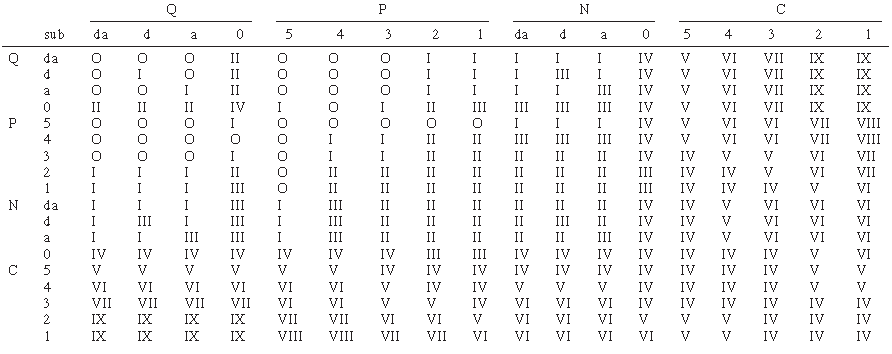
\includegraphics[width=\textwidth]{img/martiniInteractions.pdf}%
	\caption{Interaction strength association matrix for the \martini{} bead types and subtypes. Taken from \cite{Martini}.}
	\label{fig:martiniInteractions}
\end{figure}

\paragraph{\textbf{electrostatic interactions}} Electrostatic charges are assigned using the atom--centered
approximation, as described in~\ref{sec:chargeRep}. The charges of the \martini{} beads are empirically assigned at
the center of the beads and correspond to the net charge of the chemical moiety they represent. Water, for
example, is described by a neutral P$_4$ beads. Van der Waals interactions are responsible for take into account,
effectively, the effects of polarizability together with the use of an implicit medium with a dielectric constant
$\varepsilon_r = 15$. However, as we shall see in section~\ref{sec:pw}, to avoid the problems with the implicit
medium described in~\ref{sec:polarization}, especially for lipid membranes for which the dielectric constant in
the hydrophobic region is much smaller, Yesylevskyy \etal{} \cite{PW} have developed a more sophisticated \ac{CG}
water model, called \ac{PW}, to take into account a better water behavior.

\paragraph{\textbf{bonded interactions}} They include only bond length and an angle harmonic contributions. The
former is modeled with a harmonic potential as the first term in equation~\eqref{eq:bondPEF}, with the same bond
constant for all bead types: $k^b = 1250$~kJ/(mol\ nm$^2$) and an equilibrium distance of $l_0 = 0.47$~nm. The
latter is modeled as a cosine--type harmonic potential
\begin{equation}
	U = \frac{1}{2}k^a (\cos(\theta) - \cos(\theta_0))^2
	\label{eq:martiniAngle}
\end{equation}
whose parameters are: $k^a = 25$~kJ/mol and $\theta_0 = 180^\circ$ for aliphatic chains; $k^a = 45$~kJ/mol and
$\theta_0 = 120^\circ$ for \texttt{cis} double bonds and $k^a = 45$~kJ/mol and $\theta_0 = 180^\circ$ for
\texttt{trans} unsaturated bonds. Moreover, especially for ring systems, an improper dihedral angle harmonic
potential can be used to prevent out of plane distortion. The form is
\begin{equation*}
	U = k_{id} (\theta_{ijkl} - \theta_0)^2
\end{equation*}
where $\theta_{ijkl}$ denotes the angle between the planes described by atoms $i,j,k$ and $j,k,l$; $k_{id}$ and
$\theta_0$ are, as usual, the force constant and equilibrium angle.

\subsection{Simulation parameters}
The \martini{} \ac{FF} was originally developed using a shifted cut--off scheme for both Lennard--Jones and
electrostatic potentials with a cut--off radius $r_c = 1.2$~nm. The Lennard--Jones potential was shifted from
$r_s = 0.9$~nm to $r_c$ while from $r_s = 0.0$~nm to $r_c$ for the electrostatic potential. The neighbor list is
constructed as described in the first part of~\ref{sec:neighbor} with a refresh rate of $10$ \ac{MD} steps.
Recently the more efficient Verlet cut--off scheme was tested by Marrink \etal{} \cite{MartiniReview} and used
with the \martini{} \ac{FF} with a cut--off radius of $r_c = 1.1$~nm, a Verlet buffer tolerance of $0.005$~kJ/(mol\
ps) and a minimum refresh rate of $10$ \ac{MD} steps (often, depending on the hardware, it can be dynamically
increased to $30$ or $40$ \ac{MD} steps getting better performances).  Moreover, the treatment of the
electrostatic interaction can be safely updated to the \ac{PME} method together with the Verlet cut--off scheme.
This new set--up was largely tested by Yesylevskyy \etal{} \cite{PW}. In this case the cut--off radius was set to
$r_c = 1.2$~nm with the same Verlet buffer tolerance; the \ac{PME} grid spacing was set to have a lower bound of
$0.12$~nm and the interpolation was set to a fourth-order. Moreover, with the use of \ac{PW}, as we shall see,
the dielectric constant should be reduced to $\varepsilon_r = 2.5$. In all cases a time step
$20\le\delta t\le 40$ is suitable for a great number of applications. It should be clear that changing these
simulation parameters must be followed by a retest of the main properties of the \martini{} \ac{FF}.

\subsection{Parametrization}
\label{sec:martiniParam}
In order to parametrize the \martini{} \ac{CG} \ac{FF} a set of thermodynamics properties, obtained from \ac{MD}
simulations, are compared and fitted against those experimentally measured. These properties are the \textit{free
energies of vaporization}, \textit{hydration} and \textit{partitioning} between water and a set of organic
compounds such as hexadecane (H), chloroform (C), ether (E) and octanol (O). The free energy of hydration was
obtained from the partitioning of \ac{CG} beads between bulk water in equilibrium with its vapor. Similarly the
free energy of vaporization was obtained considering a simulation box with the selected \ac{CG} bead in a liquid
phase in equilibrium with its vapor. From the equilibrium densities of the particles in both phases the related
free energies can be computed from
\begin{equation*}
	\Delta G = k_B T\ln \left ( \frac{\rho_{\text{vap}}}{\rho_{\text{bulk}}} \right )
\end{equation*}
All the simulations were performed in a canonical $NVT$ ensemble.

The partitioning free energy between water and an organic solvent was obtained in a $NPT$ ensemble, considering a
simulation box half filled of water and half of the organic solvent. Then a small fraction of the \ac{CG}
particle for which the partitioning free energy is to be computed, was placed in the simulation box. From the
equilibrium densities of the particles in water $\rho_{\text{wat}}$ and in organic solvent $\rho_{\text{oil}}$,
the free energy of transfer can be computed from
\begin{equation*}
	\Delta G_{SW}^{\text{part}} = k_B T \ln \left ( \frac{\rho_{\text{oil}}}{\rho_{\text{wat}}}\right )
\end{equation*}
where $S$ indicate the organic solvent.

In figure~(\ref{fig:martiniTarget}) a summary of the results is reported. As one can see the model has bad
performances for what concerns the free energies of vaporization and hydration, which are too high with respect
to experimental data. Instead, the partitioning free energies match very well. Thus the model is not very
accurate for vapor--liquid systems but it is reliable at describing the behavior of liquid phases with
different degrees of hydrophobicity.
\begin{figure}[h!t]%
	\center
	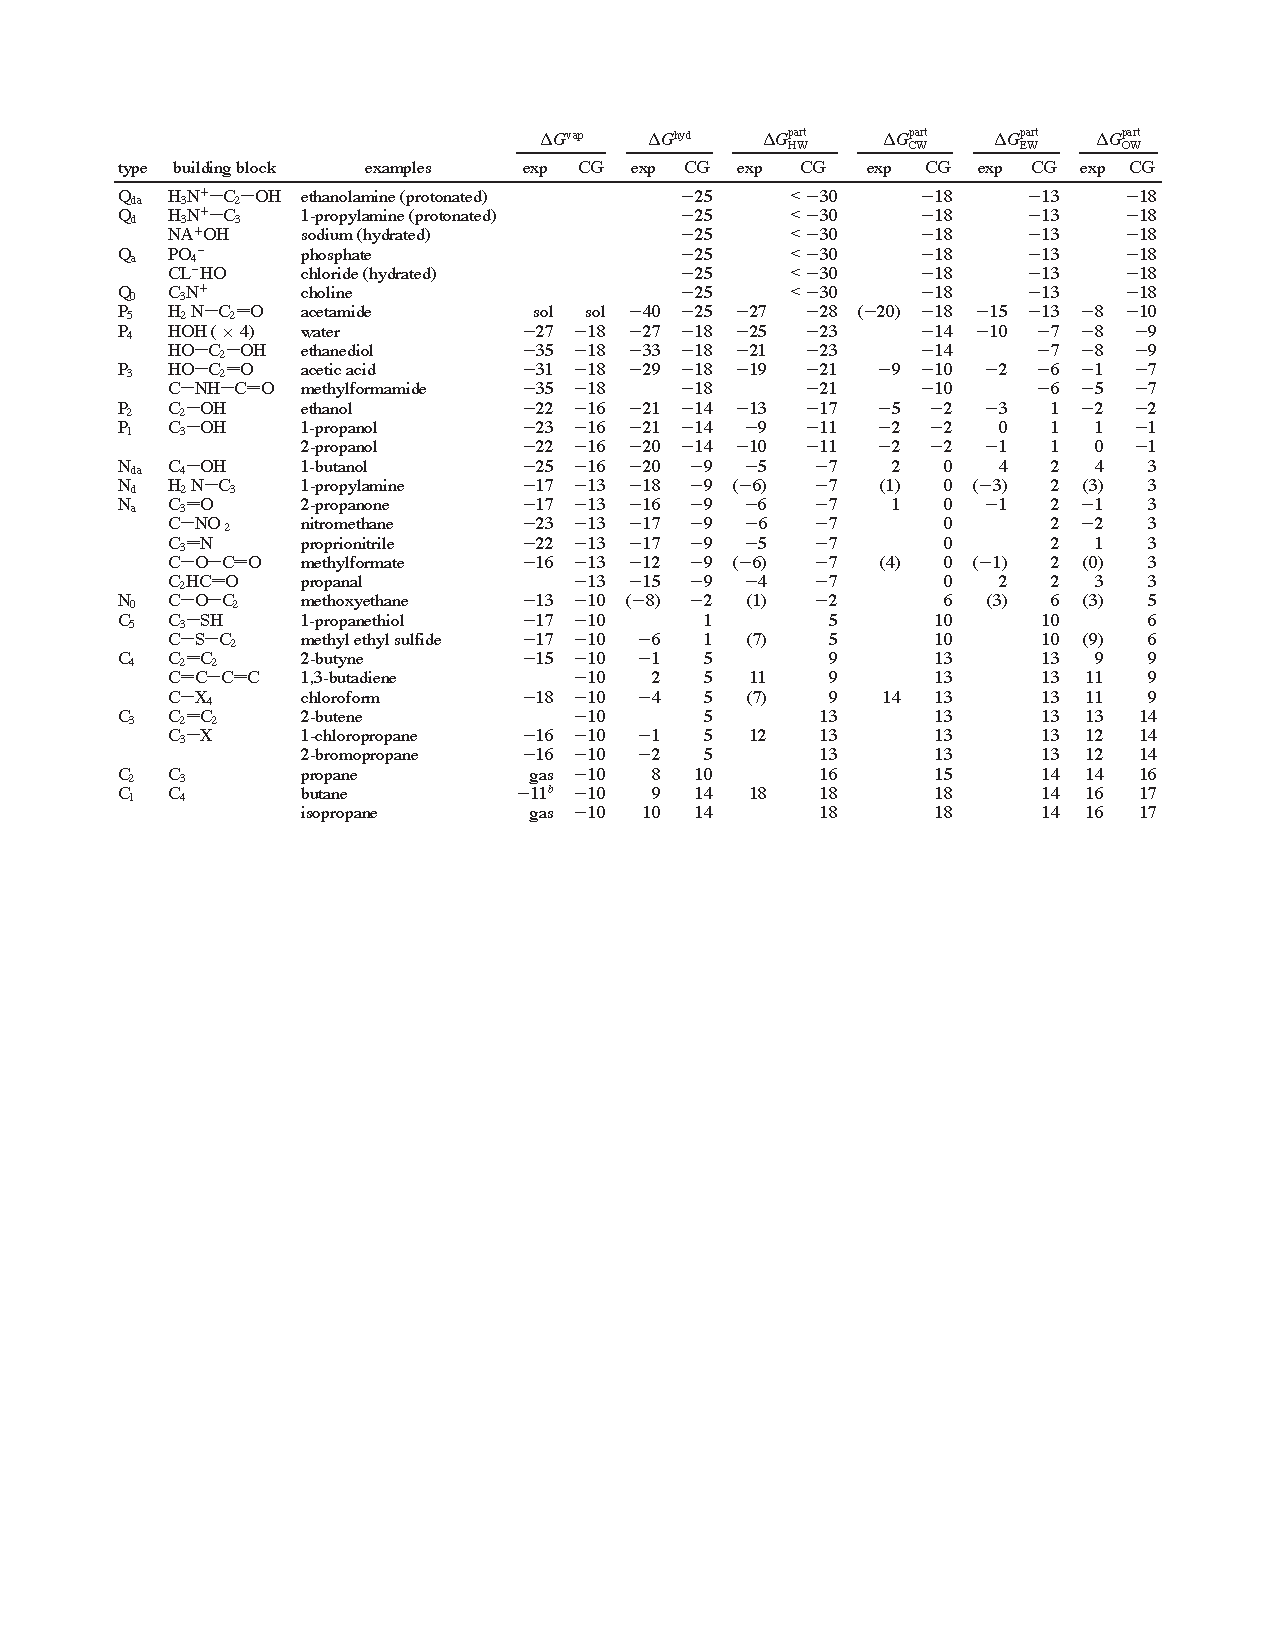
\includegraphics[width=\textwidth]{img/martiniTarget}%
	\caption{Results summary: free energies of vaporization $\Delta G^\text{vap}$, hydration $\Delta G^\text{hydr}$ and partitioning $\Delta G^\text{part}$ between water (W) and organic solvents (hexadecane (H), chloroform (C), ether (E) and octanol(O)) compared to experimental values. Experimental properties in parentheses are estimates obtained from comparison to similar compounds. The statistical accuracy of the free energies obtained from the simulations is $\pm 1$~kJ/mol. $^b$ The temperature for the experimental data is $273$~K. Taken from \cite{Martini}.}%
	\label{fig:martiniTarget}
\end{figure}

\subsection{Polarizable Water model}
\label{sec:pw}
Water plays a crucial role in any biomolecular system. It is important thus to correctly describe its behavior.
Since the \martini{} water model does not directly take into account the electrostatic interaction between water
and water and other environment because it does not have any charge and it interact only via Van der Waals
interaction, a simple implicit medium is used to take into account the main electrostatic effects of water,
screening and polarizability. In reality, however, any biomolecular process involves charged species moving
between regions of different dielectric constant. Due to the change in electrostatic screening between those
environments, the strength of the interaction between the moving charges and the surrounding molecules also
changes. This effect can not be taken into account by implicit medium models. In order to capture the
inhomogeneous nature of the dielectric response an explicit medium has to be used.
\begin{figure}[!ht]
	\centering
	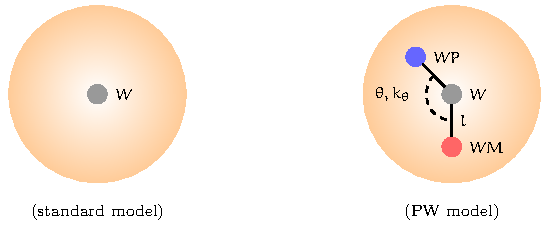
\includegraphics[width=0.7\textwidth]{./img/PWModel/PWModel}
	\caption{Schematic representation of the \acs{PW} bead. Shaded orange spheres correspond to the Van der Walls radii of the central neutral particle $W$. The blue particle is the positively charged while the red is the negatively charged.}%
	\label{fig:PW}
\end{figure}

In the same fashion of the \martini{} philosophy, Yesylevskyy \etal{} \cite{PW} have developed a \acf{PW} model
that better describes the real behavior of water. As before one \ac{PW} bead is associated to four water
molecules. The new water bead consists of three particles instead of one in the \ac{STD} \martini{} model. In
figure~(\ref{fig:PW}) the topology of the \ac{PW} and a comparison with the old model is shown. The central
particle $W$ is neutral and interacts with other particles in the system with the only Lennard--Jones potential.
There are two additional particles, namely $WP$ and $WM$, that are bound to the central particle and carry a
positive and negative charge $|q| = 0.46\mathsf{e}$ respectively, where
$\mathsf{e} = 1.60217653(14) \cdot 10^{-19}$~C is the unit electron charge. They interact with other particles in
the system by the Coulomb interaction only. The bonds $W-WP$ and $W-WM$ are constrained to have a fixed distance
$l = 0.14$~nm. The electrostatic interaction between $WP$ and $WM$ inside the same bead are exclude, thus they
are invisible to each other and they can rotate around the $W$ particle. As a consequence the dipole momentum of
the water bead depends on the relative angular position $\theta$ of $WP$ and $WM$: it can vary from zero
($\theta = 0$) to $2ql$ ($\theta = \pi$). A harmonic angle potential with equilibrium angle fixed to
$\theta_0 = 0$ and a force constant $k_\theta = 4.2$~kJ/(mol\ rad$^2$) is added to control the rotation of
$WP$ and $WM$ particles around the $W$ particle, so to adjust the distribution of the dipole momentum. The value
of the equilibrium angle is consistent with the fact that in an apolar medium the total dipole momentum of a
water molecule is zero.

Since in this model the screening and polarization effects are treated explicitly the global dielectric constant
is then reduced from $\varepsilon_r = 15$, used in the \ac{STD} \martini{}, to $\varepsilon_r = 2.5$. Moreover,
since the \ac{PW} beads attract each other stronger then the standard water beads (P$_4$ type), because of the 
additional electrostatic interactions, the strength $\epsilon_{WW}$ of the Lennard--Jones interaction between 
$W$ particles must be reduced. Water properties, especially the hydration free energy compared to the standard 
water model, and the lipid membrane behavior are reproduced satisfactory if the Lennard--Jones strength is 
changed from a $I$ level (see table~(\ref{tab:martiniEpsilon})) to a $95\%{}$ of it. Since even in this case the 
hydration free energy was too high, the same apply to the cross interaction terms between $W$ particle and the 
other \martini{} beads. Instead, $\sigma$ remains unchanged to $0.47$~nm. In addition to this, in order to recover 
the correct partitioning behavior, the self terms between Q type beads are generally decreased; while the cross 
terms are generally increased. In figure~(\ref{fig:PWMartini}) a summary of the new interaction terms between Q 
type beads and the other beads is shown.
\begin{figure}[!ht]
	\centering
	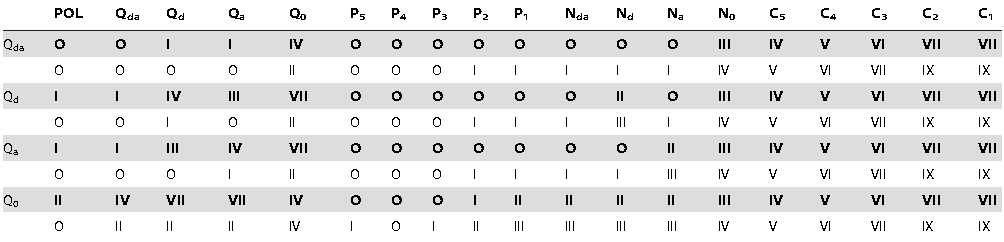
\includegraphics[width=\textwidth]{./img/PWMartini}
	\caption{New interaction strength between Q type beads and the other beads. New values in bold font, old values in normal font. See table~(\ref{tab:martiniEpsilon}) for the interaction levels. POL is the name of the \martini{} bead type associated to particle $W$ inside a $PW$ bead. Taken from \cite{PW}.}%
	\label{fig:PWMartini}
\end{figure}

The parametrization of $q$, $k_\theta$ and $\epsilon_{WW}$ are obtained, in addition to the basic target
properties of the \martini{} \ac{FF}, also trying to reproduce the dielectric constant $\varepsilon_{W}$, density
$\rho$ and dipole momentum of a pure water phase. The above parameters of the \ac{PW} model are summarized in
table~(\ref{tab:PWParam}) while a comparison of the results obtained with the \ac{PW}, the \ac{STD} \martini{}
water and the experimental data are summarized in table~(\ref{tab:PWRes}). For more details about the
parameterizations and testing methods the reader is
addressed to the article by Yesylevskyy \etal{} \cite{PW}.

Moreover, the authors found that, in addition to the \ac{PW} model, the use of \ac{PME} method contributes to a
more realistic description of the processes involved in biomolecular environments. In particular, some
interesting results of utility for this thesis work concern a better description of the properties of lipid
membranes, as we shall see in chapter~\ref{chap:membraneNP}.

\begin{SCtable}
	\centering
	\begin{tabular}{ll}
		\toprule
		$|q| = 0.46\mathsf{e}$				\\ \midrule
		$l = 0.14$~nm						\\ \midrule
		$\theta_0 = 0$						\\ \midrule
		$k_\theta = 4.2$~kJ/(mol\ rad$^2$)	\\ \midrule
		$\epsilon_{WW} = 4$~kJ/mol			\\ \midrule
		$\sigma = 0.47$~nm					\\ \bottomrule
	\end{tabular}
	\caption{Summary of the parameters used in the \acs{PW} model. See \cite{PW} for details.}
	\label{tab:PWParam}
\end{SCtable}

\begin{table}
	\centering
	\begin{tabular}{lrrr}
		\toprule
		\,	& \acs{PW} &  \martini{} water & Experimental \\ \toprule
		$\rho$~[kg/m$^3$]				& $1043$  & $1013$  & $997$		\\ \midrule
		$\overline{p}$~[D] 				& $4.9$   & $-$ 	& $4.4^a$		\\ \midrule
		$\varepsilon_{W}$ 				& $75.6$  & $-$ 	& $78.4$	\\ \midrule
		$T_\text{melt}$~[K] 			& $282$   & $290$ 	& $273$		\\ \midrule
		$\Delta G^\text{hyd}$~[kJ/mol] 	& $-18.7$ &	$-18$	& $-27$		\\ \midrule%\subsection{Applications}
		$D_{WW}~[10^{-5}$~cm$^2$/s]		& $2.5$   & $2.0$   & $2.3$		\\ \bottomrule
	\end{tabular}
	\caption{Summary of the results obtained with the \acs{PW}, \acs{STD} \martini{} water and the experimental data at $T=300$~K. $\overline{p}$ is the average dipole momentum of a pure water box and $D_{WW}$ is the self--diffusion coefficient. $^a$ In order for a comparison to be made, this data is obtained from an atomistic simulation of $1600$ SPC/E water molecules and the average dipole momentum $\overline{p}$ is obtained averaging over a groups of four molecules, randomly chosen; see \cite{PW} for more details.}%
	\label{tab:PWRes}
\end{table}

\subsection{Limitations of MARTINI FF}
As we have seen in~\ref{sec:CGModel} the \ac{CG} \acp{FF} are computationally advantageous, still a price has to
be paid. Although the \martini{} \ac{FF} is still a fine \ac{CG} \ac{FF}, some limitations are shared with other
\ac{CG} models at a fundamental level, such as the chemical and spatial resolution, which are both limited
compared to atomistic models. An important issue is the underestimation of the entropy which respect to the
atomistic case, that is a consequence of the \ac{DOF} reduction process. Since in the \martini{} \ac{FF} the
partitioning free energy $\Delta G = \Delta H - T\Delta S$ must be consistent which the experimental data, the
intrinsic loss of entropy imply a reduction of the enthalpy contribution, generating an imbalance between them.
If a $NVT$ ensemble is used the correct potential is the Helmholtz free energy $\Delta A = \Delta U - T\Delta S$,
thus the imbalance is between the internal energy and the entropy. This means that the use of a \ac{CG} model
with a $NVE$ ensemble leads to a problem of energy conservation. Anyway this is not our case since we only use a
$NVT$ or a $NPT$ ensemble with an external thermostat coupling.

Another consequence of the use of a \ac{CG} \acp{FF} is related to the \ac{FES} that becomes smoother respect to
the atomistic case. This effectively results in more sampling of the energy landscape in a given time period,
speeding up the dynamics of the system. Moreover even the \ac{PEF} becomes smoother, in particular the bonded
contributions, allowing the use of an higher time steps with longer simulation times. However the speed--up is
not easily predictable and is not likely to be the same for different systems and maybe it is dependent on the
type of molecule. Nevertheless for the \martini{} \ac{FF} an average scaling factor of four, based on lateral
diffusion coefficients of lipids in membranes, is commonly used, of course with some care. Another smaller source
of errors is due to the choice of masses: since ensemble properties are not affected by particle masses, in order
to increase the efficiency, all the \martini{} beads have the same mass of $72$~amu. This leads in some uncertainty
in the dynamics of the system making the time scaling for different beads non--trivial.

A problem involving the Lennard--Jones potential as a model of Van der Waals interactions in \martini{}, is that
the steep repulsion leads to an over--structuring of fluids compared to atomistic models. As we can see from
table~(\ref{tab:PWRes}) the direct and most evident implication is the melting point of the \acs{STD} \martini{}
water that is $290 \pm 5$~K. A practical partial solution is the use of the so called ``anti--freeze'' particles
named BP$_4$ type. The Lennard--Jones interaction between these particles and water is modified with a slightly
larger Van der Waals radius parameter, $\sigma = 0.57$~nm and a stronger interaction to be a level $O$ (see
table~(\ref{tab:martiniEpsilon}) for the interaction level). Marrink \etal{} suggest that a mole fraction of
$n_{\text{af}} = 0.1$ is sufficient to prevent freezing without affecting the other properties of water.
Using the \ac{PW} model these properties improve slightly, see table~(\ref{tab:PWRes}). For a more comprehensive
discussion about the limitations of the \martini{} \ac{FF} the reader is addressed to the review by Marrink 
\etal{} \cite{MartiniReview}.

 %Empirical Force--Field model

% !TEX root = ./../main.tex
\chapter{Model of cell membrane and monolayer--protected NP}
\label{chap:tre}
In the first part of this Chapter we present and describe the model of the charged metal monolayer--protected \ac{AuNP} developed by Federica Simonelli and co--workers in \cite{simonelliThesis} and \cite{ourPaper}, in which the \ac{AuNP} is functionalized with different ligands. The gold core is treated in a all atoms representation for future study in the photoporation context, while the ligands is modeled following the \martini \ac{CG} \ac{FF}. Then we summarize the characteristics of the cell membrane useful for this thesis work and the \martini \ac{CG} model we will use. Finally, we describe the interaction mechanism and some preliminary thermodynamic results about the interaction of the \ac{AuNP} and the model cell membrane, as outlined in \cite{ourPaper}. For a more precise discussion about the \ac{NP}--membrane interaction and the models parameterization the reader is addressed to the work of Federica Simonelli \etal\, \cite{ourPaper} and his thesis work \cite{simonelliThesis}.

\section{NanoParticle model}
% gold core --> Thyiol passivated --> ligands
%Ligand Composition: Patched (1:1), Random (1:1) (1:2)
%Different level of hydrophobicity
%Different ligand charge: anionic/cationic NP
Monolayer--protected metal \acp{NP} have the advantage of having a well defined molecular structure. That is, mono--dispersed solutions can be synthesized and structurally determined. In particular, \acp{NP} with a gold core can be stabilized by thiols\footnote{The thiol (R--SH) group is like the alcohol (R--OH) group but it is less polar respect to the second due the lower electronegativity of the sulfur respect to oxygen.}, which stably bind to the gold surface via Au-S bonds. 
%Thiolated \acp{AuNP} are air stable, electrochemically stable and thermally stable compounds [].
Several stable thiolated \acp{AuNP} are identified, differing in size of the gold core and number of ligands, see \cite{corePassivated}. In particular we consider a {Au$_{144}$(SR)$_{60}$} thiolated \ac{AuNP}, where R is the aliphatic chains of the thiol compounds; which equilibrium structure described in \cite{clusterEquilibrium}. 

Changing the composition of the aliphatic chains bonded to the thiol group, different properties of the thiolated \ac{AuNP} can be achieved, such as different net charge, different level of hydrophobicity, different size and so on. In particular, as we shall see, in the model we will use we consider only \ac{OT} and \ac{MUS} ligands that cover the \ac{NP} gold core with a monolayer with different compositions and surface arrangements. To overcome the computational cost of an atomistic model we use a \martini \ac{CG} model of the \ac{OT} and \ac{MUS} ligands. 

%The model of the \ac{AuNP} and the \martini model of the \ac{OT} and \ac{MUS} ligands are developed by Federica Simonelli \etal\, in \cite{ourPaper}, and the reader is addressed to it for a more detail discussion about the model and the parameterization.

\subsection{Passivated gold core}
% some information about gold core: dimensions, number of atoms, model used, elastic network, shel construction
The gold core is composed of $144$ atoms which displays icosahedral symmetry and it is made of three bulk shell with $12$, $42$ and $60$ atoms, respectively. A surface shell of $30$ atoms completes the gold cluster structure. Then $60$ sulphur atoms, which blind the aliphatic chains (R) to the gold core, are bounded to the gold atoms on the surface through the typical bond structure RS--Au--SR. The shell construction is shown in figure~(\ref{fig:goldShell}).
\begin{figure}[!ht]
	\centering
	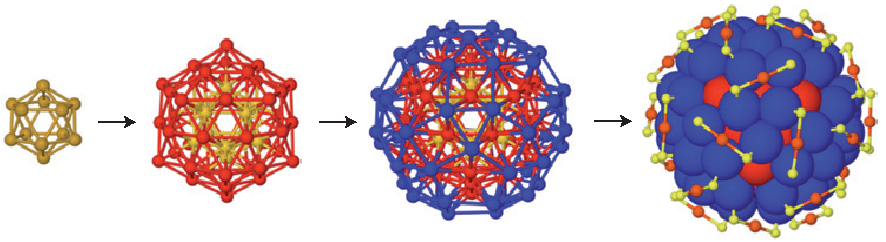
\includegraphics[width=0.8\textwidth]{./img/goldShell}
	\caption{First three frame: the concentric $12$--(yellow), $42$--(red) and $60$--(blue) atom gold internal shell, surrounded (last frame) by $30$ gold (red small) and $60$ sulphur (yellow small) surface atoms. The R chains is not shown. Taken from \cite{corePassivated}.}
	\label{fig:goldShell}
\end{figure}

The resulting diameter of the gold core is about $2$~nm. When passivated by thiols, its overall size depends on the length of the aliphatic chains bound to the sulphur atoms. The monolayer--protected \ac{AuNP} we will consider have a total diameter of about $4$~nm.

\paragraph{\textbf{gold elastic network}} Despite the computational cost associated to atomistically describe the gold cluster, all gold atoms are taken into account in order to allow us future studies on heating effect on lipid bilayer. Thus the bonds between gold atoms are allowed to vibrate. As we have seen in a previous section, a many--body potential should be used. Instead, as we are interested in the vibrational modes of the core atoms, 
%Federica Simonelli in her thesis work, found that
a more efficient way is to use an elastic network associate the potential energy
\begin{equation*}
	U = \frac{1}{2}\sum_i \sum_{j\ne i}k_{ij}(r_{ij} - r_{ij}^0)^2
\end{equation*}
where $r_{ij}$ is the distance and $k_{ij}$ is the bond constant for $i-j$ atom pair. 
%The bond constants is assigned so as to reproduce the vibrational spectrum of the gold core as provided by the many--body Gupta potential. 
The bond constant is assigned to $k = 32500$~kJ/(mol\,nm$^2$) for surface atoms and $k = 11000$ kJ/(mol\ nm$^2$) for bulk atoms. While the equilibrium distances are derived from \cite{clusterEquilibrium}. A gold atom is considered as bulk atom if it has at least nine gold atom neighbors otherwise as a surface atom. A gold atom is considered neighbor to another if it lie within a shell of radius $0.35$~nm centered to the considered atom. In figure~(\ref{fig:goldNetwork}) the gold elastic network is shown.
\begin{SCfigure}[][ht]
	\centering
	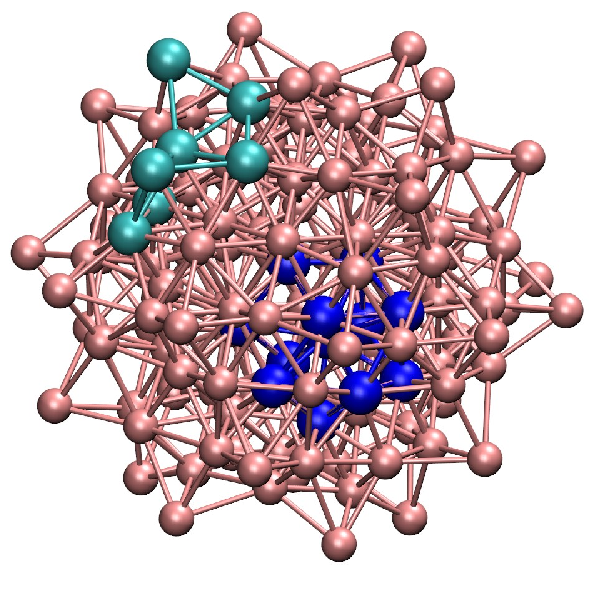
\includegraphics[width=0.35\textwidth]{./img/goldNetwork}
	\caption{Elastic network, represented by the stick bond, among gold atoms (pink). In cyan a surface atoms and its neighbors. In blue a group of bulk atoms and its neighbors. Taken from \cite{simonelliThesis}.}
	\label{fig:goldNetwork}
\end{SCfigure}

\paragraph{\textbf{sulfur elastic network}} An elastic network, with bond constant of $1250$~kJ/(mol\,nm$^2$) and equilibrium distances derived from \cite{clusterEquilibrium}, is also used to model sulphur atoms on the surface of the \ac{NP} cluster. A cutoff distance of $0.55$~nm is used to select the sulphur neighbor atoms, i.e. each sulfur atom have at least five neighbors. The interaction between a sulphur atom and its nearest gold atoms is modeled through a harmonic potential with a bond constant of $32500$~kJ/(mol\,nm$^2$) and equilibrium distances given by \cite{clusterEquilibrium}. In order to prevent the penetration of the sulphur atoms into gold core, a repulsive potential of the form $C/r^{-12}$ where $C = 0.92953\cdot 10^{-6}$~(kJ\,nm$^{12}$)/mol models the non--bonded interaction between gold and sulphur atoms which are not involved in any of the previous bonds. In figure~(\ref{fig:NPCluster}) sulphur passivated \ac{AuNP} cluster with the complete elastic network is shown. 
\begin{SCfigure}[][h]
	\centering
	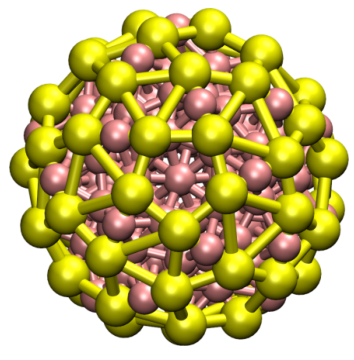
\includegraphics[width=0.35\textwidth]{./img/NPCluster}
	\caption{The \acs{AuNP} cluster. Gold atoms are in pink and sulfur atoms in yellow. The elastic network for both gold and sulfur atoms are represented by sticks. Taken from \cite{ourPaper}.}
	\label{fig:NPCluster}
\end{SCfigure}

\subsection{Functionalizing ligands}
Our \ac{AuNP} core is functionalized with \ac{MUS} and \ac{OT} ligands. The former is a charged compounds made of eleven \ac{CH2} groups and a charged terminal \ac{SO4-} group. The charged terminal group make it partially hydrophilic. The latter, instead, is completely hydrophobic and it is made by seven \ac{CH2} groups and one \ac{CH3} terminal group. Using both hydrophilic and hydrophobic groups guarantees that such \acp{NP} are stable, that is, does not aggregate, in both aqueous and non--aqueous environments.

%\subsection{OT ligands}
\paragraph{\textbf{OT Model}} Two \martini beds of type C$_1$ model the eight carbon atoms of the \ac{OT} backbone and their hydrogen atoms. The chemical structure and the resulting \ac{CG} \martini model is shown in figure~(\ref{fig:ot}). The first bead of each \ac{OT} ligands is bound to a sulphur atom via a harmonic potential with a bond constant of $1250$~kJ/(mol\,nm$^2$) and equilibrium length of $0.47$~nm. The second bead is connected to the first by the same bond potential. An angle potential as in equation~\eqref{eq:martiniAngle} is used among the three particles. Parameters are fixed in accordance with the standard \martini ones (see section~\ref{sec:martiniPotential}). Moreover a purely repulsion potential, as described previously, is used between C$_1$ beads and gold and sulfur atoms to prevent the co--penetration.
\begin{figure}[!ht]
	\centering
	\subfloat[\acs{OT} ligand]{%
		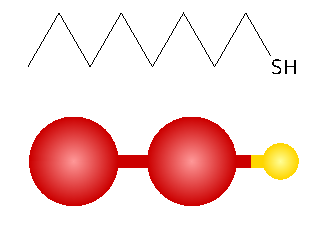
\includegraphics[width=0.3\textwidth]{./img/OT/OT}%
		\label{fig:ot}%
	}%
	\qquad\qquad%
	\subfloat[\acs{MUS} ligand]{%
		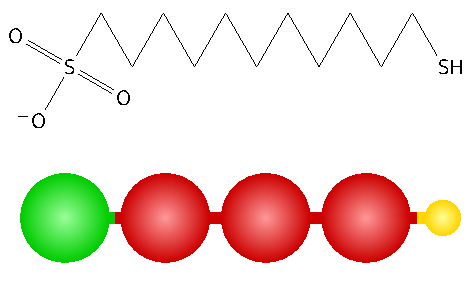
\includegraphics[width=0.35\textwidth]{./img/MUS/MUS}%
		\label{fig:mus}%
	}%
	\caption{Top: chemical structure. Bottom: \acs{CG} \martini model (red: C$_1$ bead, green: Qda negatively charged bead and yellow: sulfur atom).}
\end{figure}

%\subsubsection{MUS ligands} %Anionic an the cationic???
\paragraph{\textbf{MUS Model}} Three \martini beads of type C$_1$ model the hydrophobic chain of the \ac{MUS} ligand. The charged group is modeled as a Qda beads with a charge of $-\mathsf{e}$. The chemical structure and the resulting \ac{CG} \martini model is shown in figure~(\ref{fig:mus}). Even in this case the first bead of a \ac{MUS} ligand is bounded to the sulphur atom through a harmonic potential with the same parameter: bond constant of $1250$~kJ/(mol\,nm$^2$) and equilibrium length of $0.47$~nm. The same potential is used to bind all other beads to the previous one. An angle potential as in equation~\eqref{eq:martiniAngle} is used among the sulfur atom, the first C$_1$ and second C$_1$, among the first, the second and the third C$_1$ beads and so on for all four beads. Parameters are fixed in accordance with the standard \martini ones (see section~\ref{sec:martiniPotential}). As in the \ac{OT} ligand model, a purely repulsion potential, as described previously, is used between C$_1$ beads and gold and sulfur atoms to prevent the co--penetration. The same applies between Qda bead and gold and sulfur atoms.

\paragraph{\textbf{level of hydrophobicity}} The \ac{AuNP} core can be functionalized with both ligands in different composition. In particular varying the ratio between the \ac{OT} and \ac{MUS} ligands different levels of hydrophobicity can be reached: it decrease augmenting the number of charged ligands. Two surface composition is considered: (\ac{MUS}:\ac{OT} $1$:$1$) and (2:1), the former is the main used in this thesis work.

\paragraph{\textbf{surface arrangements}} The arrangements of the ligands on the \ac{AuNP} surface can be made in two possible way: randomly or with a predetermined scheme. In particular for the second possibility we use a striped scheme: the \ac{NP} surface is divided in three strips, the external two strips are covered with \ac{MUS} ligands while the central with \ac{OT} ligands. For this thesis work we consider three type of \ac{NP}: striped (\ac{MUS}:\ac{OT} $1$:$1$), random (\ac{MUS}:\ac{OT} $1$:$1$) and random (\ac{MUS}:\ac{OT} $2$:$1$). In figure~(\ref{fig:coating}) the different coatings for the \ac{NP} core is shown.

\begin{figure}[!ht]
	\centering
	\subfloat[striped ($1$:$1$)]{
		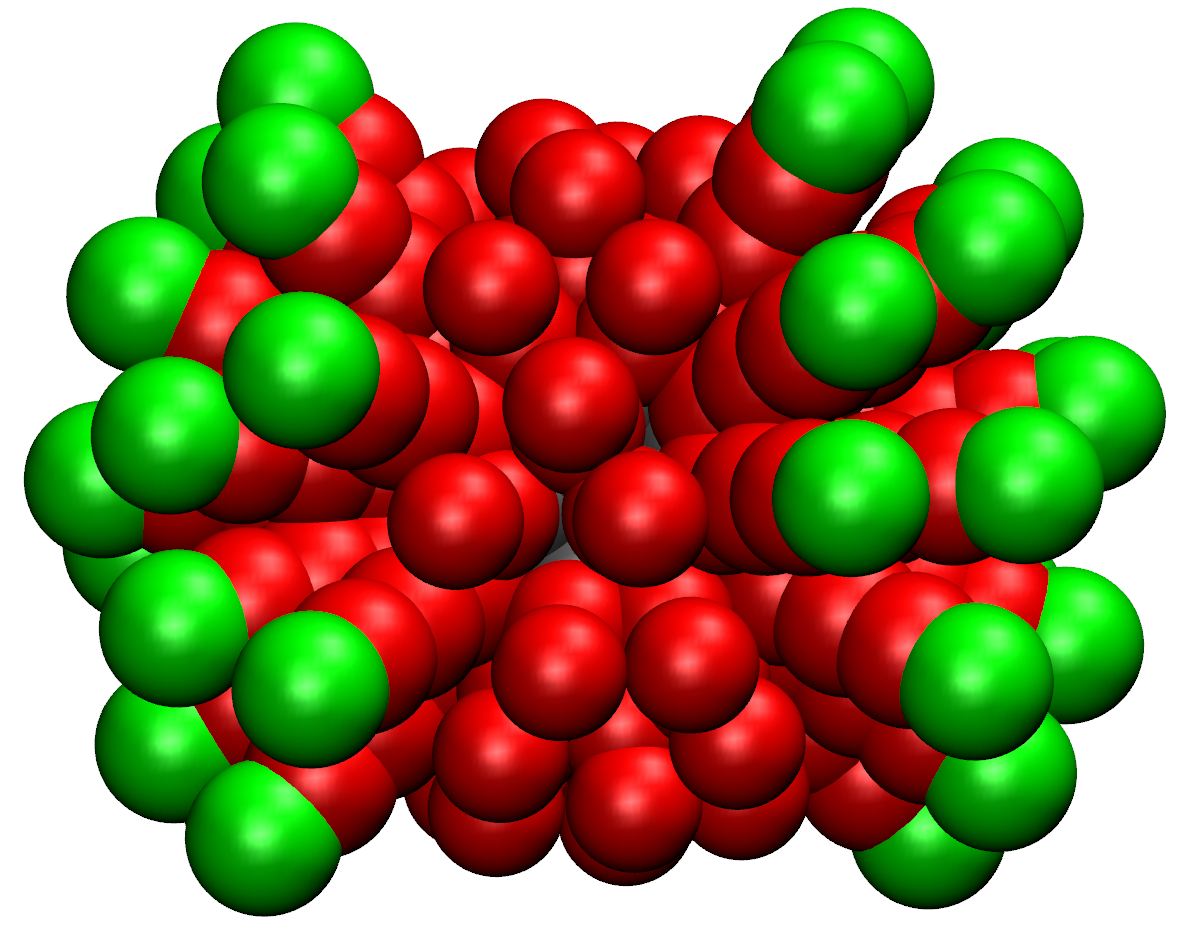
\includegraphics[width=3.3cm]{./img/coatings/striped}
	}%
	\qquad
	\subfloat[random ($1$:$1$)]{
		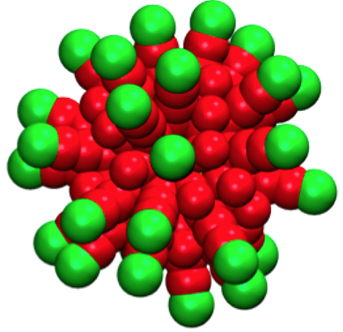
\includegraphics[width=2.9cm]{./img/coatings/random11}
	}%
	\qquad
	\subfloat[random ($2$:$1$)]{
		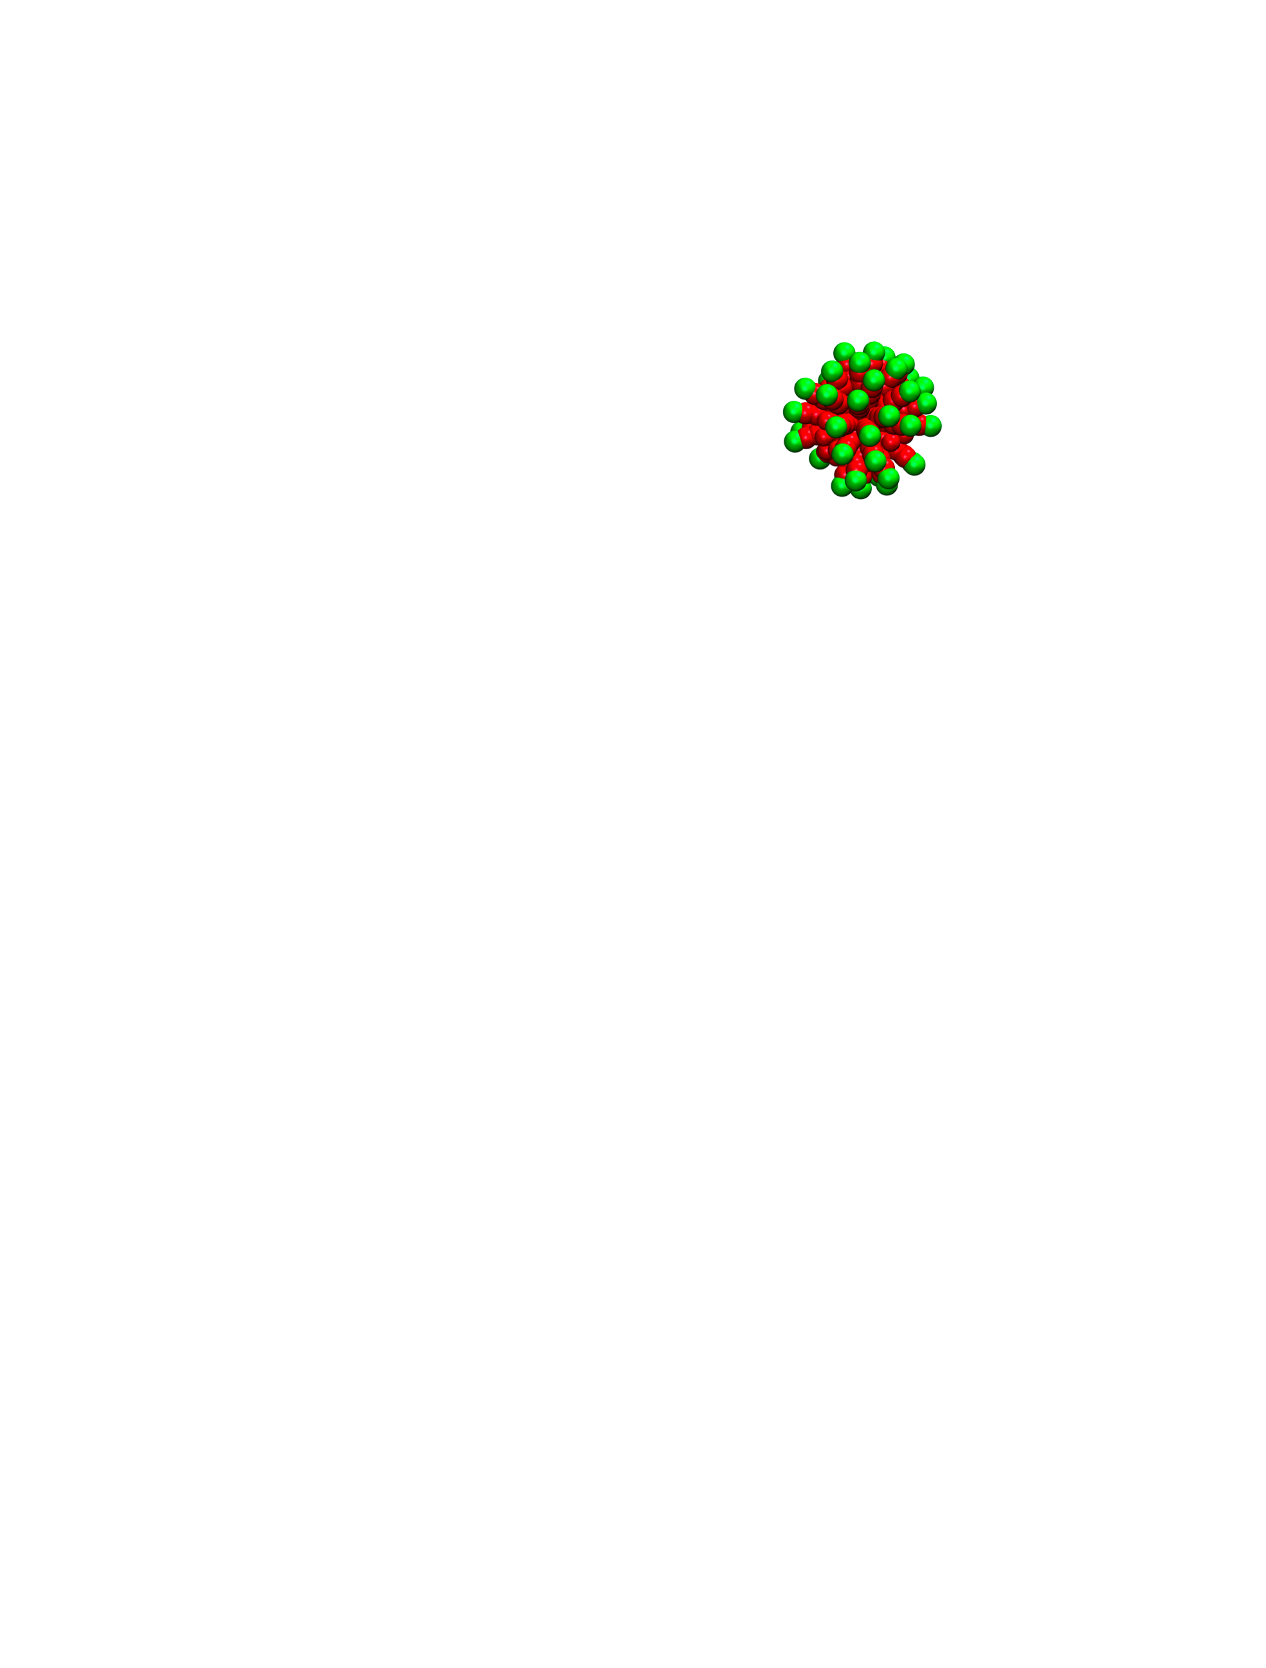
\includegraphics[width=2.7cm]{./img/coatings/random21}
	}%
	\caption{Au\acs{NP} with different ligands surface arrangements and composition. From left to right: striped (\ac{MUS}:\ac{OT} $1$:$1$), random (\ac{MUS}:\ac{OT} $1$:$1$) and random (\ac{MUS}:\ac{OT} $2$:$1$). Hydrophobic beads are shown in red while the negatively charged beads are green.}
	\label{fig:coating}
\end{figure}

\section{Cell membrane}

\subsection{Real cell membrane}
The cell membrane or cytoplasmic membrane is a biological membrane that separate the interior and the external environments of a living cells. The basic function is to protect cells from its surroundings but it also takes the function of a ``customs'' in order to allow the cells to exchange chemical compounds from and to the external environment. To fulfill at this role the cell membrane is a crowded environment consisting of phospholipids, glycolipids, carbohydrates proteins and so on as we can see from figure~(\ref{fig:cellMembrane}).
\begin{figure}[!ht]
	\centering
	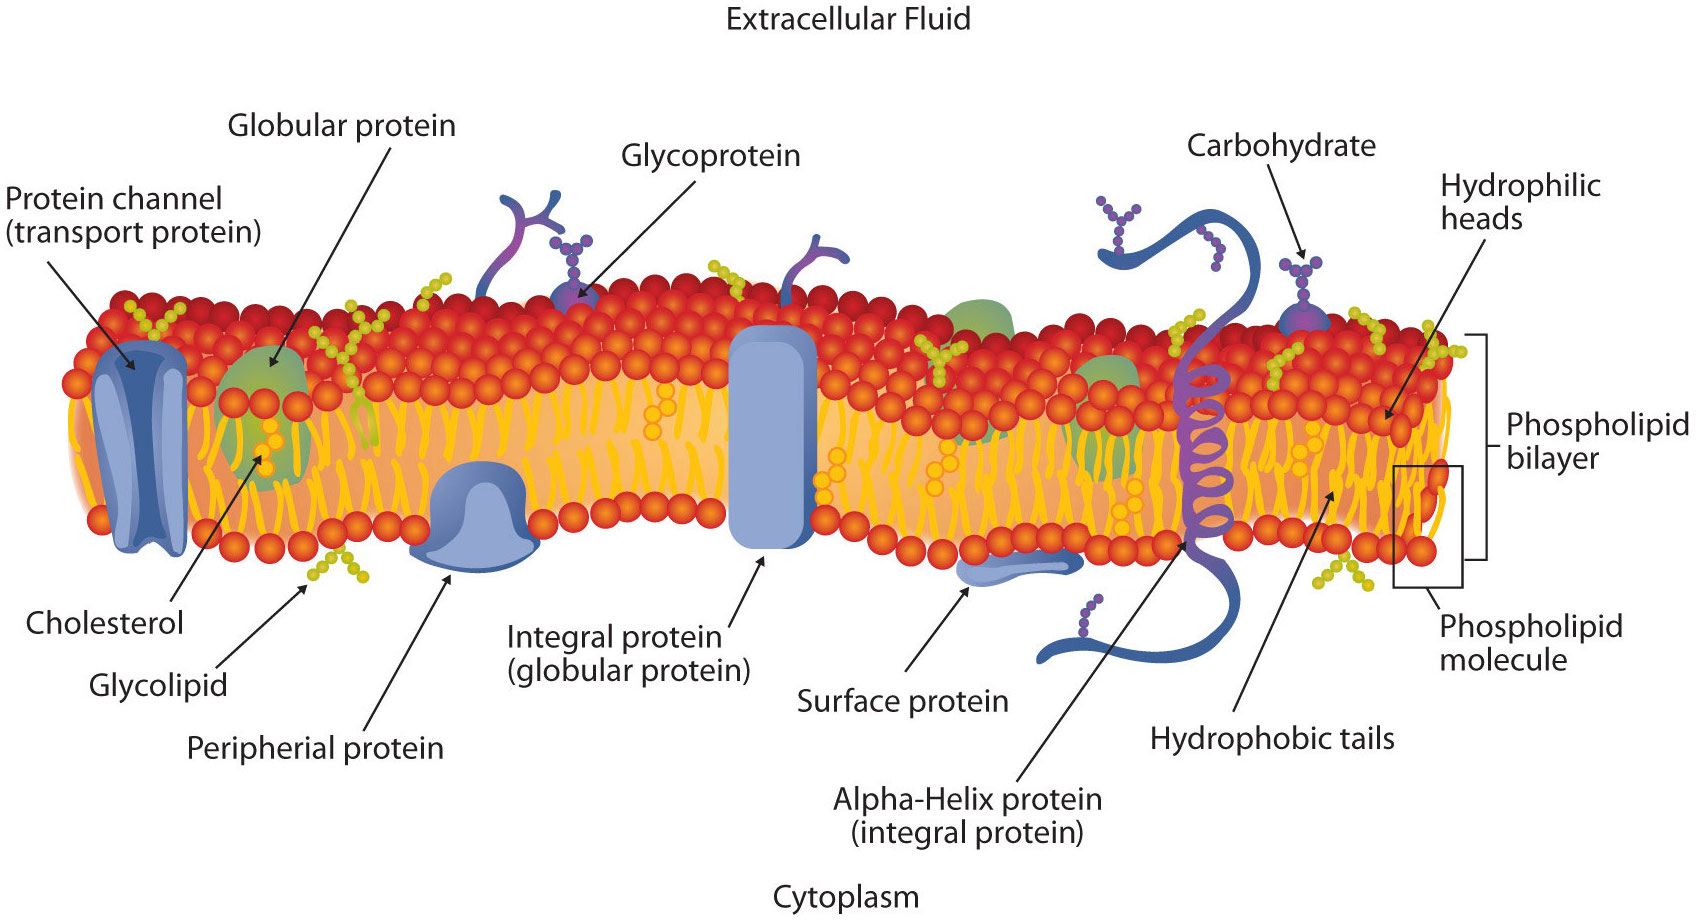
\includegraphics[width=0.9\textwidth]{./img/cellMembrane}
	\caption{Schematic representation of a biological cell membrane.}
	\label{fig:cellMembrane}
\end{figure}

The skeleton of a cell membrane is a bilayer sheet made of \textit{phospholipids}. They are a kind of lipids made of a polar or charged head, which is hydrophilic and one or two fatty acid hydrocarbon chains, often called lipid tails, which are instead hydrophobic; phospholipids are then amphiphilic molecules. This amphiphilic nature play a key role in the bilayer formation. In fact the formation of a bilayer in water is a self--assembly process driven by the hydrophobic effect which acts so as to minimize the number of hydrophobic contact between water and lipid tails. Moreover the bilayer sheet is not the only possible structure, based on the concentration of the phospholipids in water and on the temperature the self--assembly process can lead to three main different structures: bilayer sheet, liposome and micelle. In figure~(\ref{fig:lipidsStructures}) a schematic representation of this three different structures is shown.
\begin{SCfigure}[][!ht]
	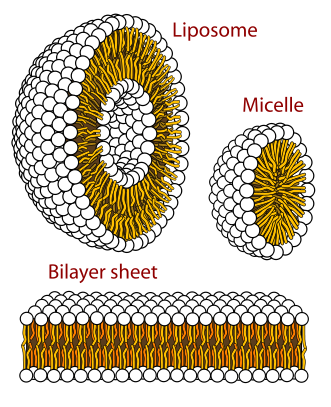
\includegraphics[width=0.3\textwidth]{./img/lipidsStructures}
	\caption{Cross--section view of the structures that can be formed by a self--assembly process of phospholipids in aqueous solution.}
	\label{fig:lipidsStructures}
\end{SCfigure}

A real lipid bilayer often contains hundred of different lipid species. They differ in the length of the hydrocarbon chains, in the degree of unsaturation, i.e. in the number of double bond in the hydrocarbon chains, and in different composition of the head that can be polar or non--polar. There are two main classes of phospholipids that make a cell membrane of animals: glycerophospholipid (phosphatidyl--choline, phophatidyl--ethanolamine, phophatidyl--serine, phosphatidyl--serine ) and phosphosphingolipids (sphingomyelin). In the former group the lipid tails are bound to a glycerol group while the latter do not have glycerol and the lipid tails have a backbone of sphingoid bases, absent in the former. These five types take into account for more then half of the lipids in most membranes.

The cell membrane has a quasi--liquid properties at physiological temperature. This is in part due to some disorder in the alignment of the lipid tails produced by the presence of unsaturated chains. Another contribution arise from the area occupied by the lipid heads which determines the distance between the hydrocarbon chains. This fluid character make the lipid bilayer like a solvent in which the other molecules are dissolved (lipids and proteins) and are free to diffuse. Moreover the lipids itself can move in different ways. The main movements and the associated time scales are summarized as follow
\begin{itemize}
	\item lipids conformational change (few nanoseconds);
	\item lipids protrusions out--of--plane (tens of picoseconds);
	\item diffuse within a leaflet (order of tens of nanoseconds);
	\item bilayer undulation and thickness involve collective motion of many lipids.
\end{itemize}
There are also many rare events that take place on the order of hours or even days, such like lipid flip--flop, in which a lipid go to the opposite leaflet; ions translocation; \textit{electroporation} by water, for example due to a cross membrane ions imbalance, in which water penetrate inside the bilayer and destroys a small portion in order to come to the other leaflet; water--helped ions permeation, called \textit{water--finger} and more general water defects inside the membrane.

For what concern the length scales, the bilayer thickness is determined by the length of the lipid tails and their degree of unsaturation. Typically the hydrophobic region is $\sim 3$~nm thick while each hydrophilic regions is $\sim 1$~nm thick. Hence the typical bilayer thickness is around $\sim 4\div 5$~nm.

\subsection{Model cell membrane}
As we have seen above, the cell membrane is an extremely complex environment due to the large number of different species and lipids which composes and resides in the bilayer sheet. The most common simplification in order to develop a model to use in a \ac{MD} simulation at atomistic or \ac{CG} level, consist to considers only one specie of phospholipid and no other compounds. In the bilayer model we will use in this thesis work, we consider model biological membrane consisting of \ac{POPC}. It is a zwitterionic glycerophospholipid of type phosphatidyl--choline whose head is made of a phosphate (PO$_4^-$) and a choline (C$_5$H$_{14}$NO$^+$) groups. It has two hydrocarbon chains: one is a saturated chain (palmitoyl) and the other is an unsaturated chain (oleoyl). The head groups and tails are both bounded to the glycerol group (C$_3$H$_8$O$_3$). In the top of figure~(\ref{fig:popc}) the chemical structure of the \ac{POPC} lipid is shown.

It is clear that the number of lipids that constitute a real cell membrane is enormous and it is extremely hard to take into account an entire cell membrane in a \ac{MD} simulation. A first approximation is to consider only a small area of the model bilayer. Given the medium area per lipid of about $0.65$~nm$^2$ and a portion of bilayer of $\sim 160$~nm$^2$, which corresponds to about $250$ lipids per leaflet, the total number of particles to be included in a atomistic simulation (excluding hydrogen atoms) are about $26\cdot 10^3$ plus the water molecules ($\sim 60\cdot 10^3$). This has a very expensive computational cost and the range of phenomena which can be studied on these time and length scales are very limited, calling for the adoption of a \ac{CG} approach.

\begin{figure}[!ht]
	\centering
	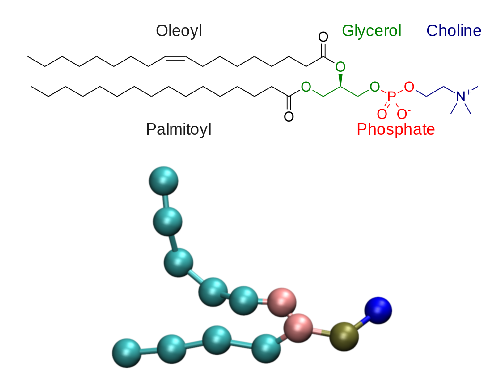
\includegraphics[width=0.7\textwidth]{./img/POPC/popc}
	\caption{Top: chemical structure of a \acs{POPC} lipid. Bottom: \martini \acs{CG} model. The tan bead is the phosphate group, choline is in blue, the two pink beads represents the glycerol group and the hydrophobic chains in cyan.}
	\label{fig:popc}
\end{figure}

\paragraph{\textbf{martini model}} As described in section \ref{sec:martini}, in this thesis work we use the \martini \ac{FF} for \ac{CG} lipids \cite{Martini}. The authors have developed a well suitable and comprehensive model about \ac{POPC} and a large variety of lipids. We consider a lipid bilayer made of $512$ \ac{POPC} lipids which extend on a surface of about $160$~nm$^2$ and whose thickness is about $4$~nm. The \martini model for the \ac{POPC} lipid maps the choline and the phosphate groups into two beads of type Q$_0$ and Qa negatively and positively charged, respectively. The saturated tail is modeled with four beads of type C$_1$ while the unsaturated tail is built up of four C$_1$ beads and one C$3$ bead which corresponds to the unsaturated group of atoms. The glycerol group is modeled with two beads of type N$_\text{a}$. A comparison between the chemical structure and \ac{CG} model is shown in figure~(\ref{fig:popc}).

\paragraph{\textbf{model comparison}} The standard \martini \ac{FF} is able to capture the main aspects of the physical properties of a lipid bilayer with less computational effort respect to an atomistic simulation. These properties are the area per lipid, the lipid diffusion constant, the distribution of groups across the membrane, the bending and the area compression moduli, the stress profile across the membrane and many other as described in the original work by Marrink \etal\, \cite{Martini}. Nevertheless many other properties, prevalently mediated by the electrostatic interaction, are not well described. As we have seen in the previous Chapter this is because the \martini \ac{FF} does not take into account the long range treatment of the electrostatic interaction and because the standard \martini water is prevalently insensible to the electrostatic interaction\footnote{Moreover we can not forget that the \martini water bead takes into account four real water molecules. Hence the probability for a \martini water bead to permeate the hydrophobic region of the membrane is much less then for a water molecule in an atomistic \ac{FF}.}. To overcome to this problem the use of the \ac{PW} model and the \ac{PME} method, as outlined in \cite{MartiniReview} and \cite{PW}, are crucial to better describe the aforementioned process that involve lipid bilayer, water and charged ions. These are ions translocation; electroporation of the membrane by water, due to a cross membrane ions imbalance; water--helped ions permeation and many other water defects inside the membrane as better described in the works of Marrink and Yesylevskyy.

\paragraph{\textbf{ions translocation}} An important phenomenon mediated by the electrostatic interactions that is crucial for this thesis work is the lipid membrane ions translocation. In \cite{PW} the authors have computed the \ac{FES} of the translocation of Na$^+$ and Cl$^-$ ions\footnote{The \martini model for Na$^+$ and Cl$^-$ associates the ion plus the hydration shell to a bead of type Qd positively charged and Qa negatively charged, respectively.} across a \acs{DPPC} membrane using umbrella sampling and the \ac{WHAM} with the standard \martini \ac{FF}, adding the \ac{PW} and adding together \ac{PW} and \ac{PME}. The height of the barriers are summarized in table~(\ref{tab:ionTranslocation}). The same \ac{FES} for a \acs{DMPC} membrane was calculated by Khavrutskii \etal\, \cite{atomisticTranslocation} with an atomistic \ac{FF}. Since the \martini model for the \acs{DPPC} lipid also model the \acs{DMPC} lipid a comparison can be made and it is shown in table~(\ref{tab:ionTranslocation}). As one can see, from left to right, increasing the loyalty of the treatment of the electrostatic interaction the \martini \ac{FF} approach the results of the atomistic \ac{FF}. Moreover in \cite{PW}, in accordance with the atomistic results in \cite{atomisticTranslocation}, only with the use of the \ac{PW} model and the \ac{PME}. for small cross membrane ions imbalance, they observe some ion leakage without pore formation but still mediated by a water defect inside the membrane, called \textit{water finger} that help the ions to cross the hydrophobic region of the membrane. These phenomena are totally absent using the standard \martini \ac{FF}. Hence, as already outlined, the importance to use a better treatment of the electrostatic interaction.
\begin{table}[h!t]
	\centering
	\begin{tabular}{lcccc}
		\toprule
		\,		& Standard & \acs{PW} & \acs{PW} \& \acs{PME} & Atomistic	\\ \toprule
		Na$^+$	& 68.0	   & 67.6	  & 78.6					& 91.7 		\\ \midrule
		Cl$^-$	& 69.2	   & 70.4	  & 99.0					& 98.8		\\ \bottomrule
	\end{tabular}
	\caption{Height of the energy barrier (in kJ/mol) for Na$^+$ and Cl$^-$ translocation across a bilayer. The \martini results are based on a \acs{DPPC} membrane and are taken from \cite{PW} while the atomistic are based on a \acs{DMPC} membrane and are taken from \cite{atomisticTranslocation}.}
	\label{tab:ionTranslocation}
\end{table}

\section{NP--Membrane interaction}
Recently the literature for what concern the computational modeling about the interaction of such anionic monolayer--protected \ac{AuNP} and model lipid membranes has expanded contributing to sketch a possible mechanism of such interaction. The begging of the path way mechanism is the electrostatic attraction between the charged ligands and the polar head of the zwitterionic phospholipids in a fluid water phase: it is recognized to be the driving force for the adhesion of the \ac{AuNP} to the membrane surface, see figure~(\ref{fig:threeProcess}a). To the other end of the path way, it is known, on thermodynamic basis, that the most stable state for the \ac{AuNP} corresponds to the so--called \textit{snorkeling} configuration in which the \ac{NP} is embedded in the hydrophobic region of the membrane, while the charged ligands stably interact with the lipid heads of both leaflets, see figure~(\ref{fig:threeProcess}f). 

In the work of Federica Simonelli \etal\, \cite{ourPaper}, using the just described \ac{CG} \martini models of the \ac{NP} ligands and of biological membrane, with the standard \martini \ac{FF}, they found and characterize a possible path way mechanism of the interaction process with membrane at low curvature. Then they perform metadynamics simulations for characterize the thermodynamic of the process.

\paragraph{\textbf{Three--stage process}} The authors found a three--stage mechanism that regulate the insertion of the \ac{AuNP} into the membrane core: from the adsorbed state, figure~(\ref{fig:threeProcess}a), to the snorkeling configuration, figure~(\ref{fig:threeProcess}f). When the \ac{NP} in the water phase approach the surface of the membrane it enters in the Stage $1$ or in the adsorbed state in which the charged ligands interact with the polar lipid heads. Then, in Stage $2$, a key role is played by a lipid tail protrusion out of the hydrophobic region that stably interact with the hydrophobic beads of the \ac{NP} ligands, see figure~(\ref{fig:threeProcess}b-c). In order to minimize the contacts between water and the tails of the protruding lipid it pull the \ac{OT} ligands into the membrane core and the \ac{NP} enter in the hydrophobic contact state, figure~(\ref{fig:threeProcess}d). Then due the thermal fluctuation a charged bead is involved to cross the membrane core and stably interact with the head region of the opposite leaflet, figure~(\ref{fig:threeProcess}e).
\begin{figure}[hb]
	\centering
	\subfloat[]{
		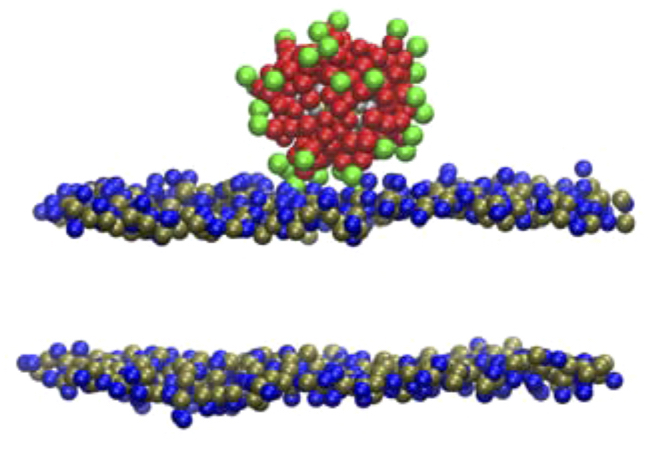
\includegraphics[width=4cm]{./img/threeProcess/a}
	}%
	\quad%
	\subfloat[]{
		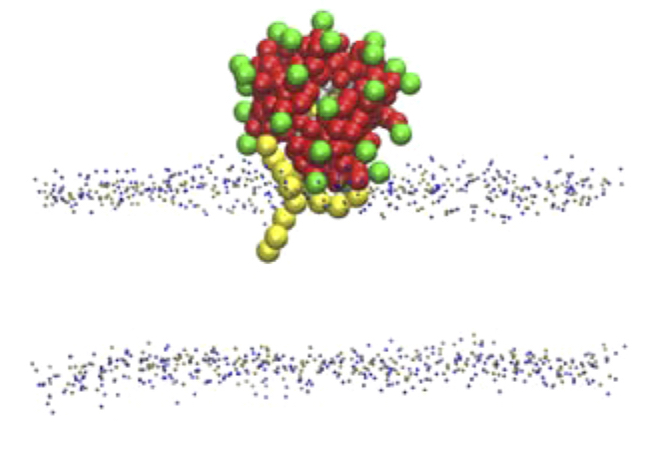
\includegraphics[width=4cm]{./img/threeProcess/b}
	}%
	\quad%
	\subfloat[]{
		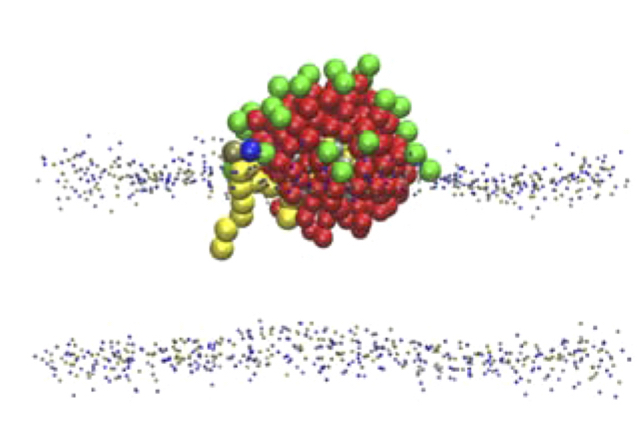
\includegraphics[width=4cm]{./img/threeProcess/c}
	}%
	\\%
	\subfloat[]{
		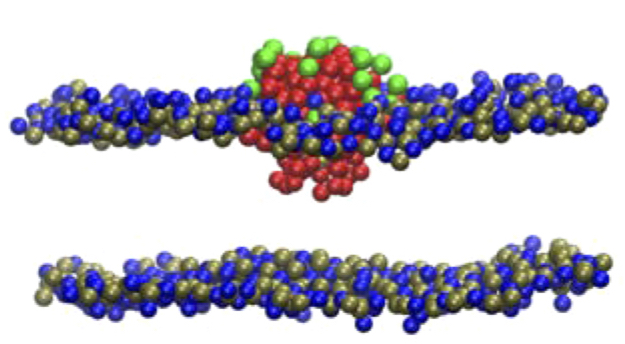
\includegraphics[width=4cm]{./img/threeProcess/d}
	}
	\subfloat[]{
		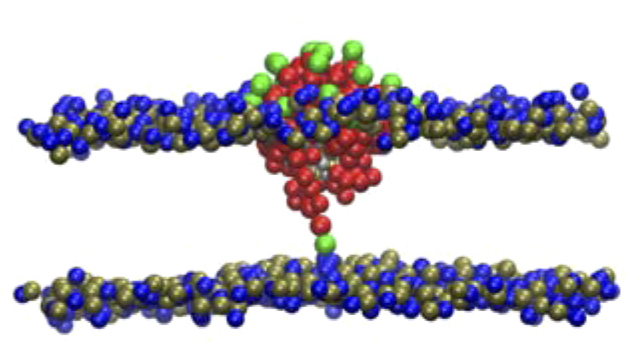
\includegraphics[width=4cm]{./img/threeProcess/e}
	}%
	\quad%
	\subfloat[]{
		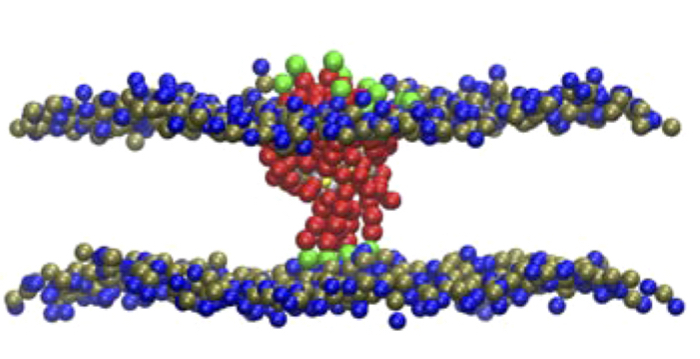
\includegraphics[width=4cm]{./img/threeProcess/f}
	}%
	\caption{\acs{AuNP}--membrane interaction. (a) Stage $1$, adsorption of the \acs{NP} at membrane surface; (b) to (d) Stage $2$, the protrusion of a lipid tail initiates the hydrophobic contact that leads to partial embedding of the \acs{NP} in the membrane core; (e) the \ac{NP} binds to the opposite leaflet throwing a charged ligand; (f), Stage $3$, snorkeling configuration (five anchors shown). The hydrophobic beads of the ligands are shown in red and the charged beads in green. Lipid heads are blue (choline) and tan (phosphate), lipid tails are not shown, expect for (b) and (c), where the protruding lipid is shown with yellow tails. Water beads are not shown. All snapshot refer to a random (\ac{MUS}:\ac{OT} $1$:$1$) configuration. Taken from \cite{ourPaper}.}
	\label{fig:threeProcess}
\end{figure}
Since the anchored state is thermodynamically favorable respect to the hydrophobic contact, more and more ligands drop the charged beads to the head region of the opposite leaflet, approaching step--by--step the snorkeling configuration, figure~(\ref{fig:threeProcess}f). Moreover, compatibly with other works in literature, they found that the energy cost associated with the extraction of the \ac{NP} out of the membrane core is very high, making the anchoring process, and the snorkeling configuration, almost irreversible.
 
\bigskip
The authors performed \ac{MD} simulations for the three different \ac{NP} configurations showed in figure~(\ref{fig:coating}): the striped (\ac{MUS}:\ac{OT} $1$:$1$), the random (\ac{MUS}:\ac{OT} $1$:$1$) and the random (\ac{MUS}:\ac{OT} $2$:$1$). They found that the described behavior is common to the three configurations. Moreover, the lipid tail protrusion mechanism is validate form the kinematic of the simulations: the energy barrier to be overcome to move from stage $1$ to stage $2$ is of the order of the estimated energy cost of a lipid tail protrusion. Nevertheless, after the hydrophobic contact is reached, its lifetime depends on the surface ligand arrangements. For the random configurations the time lag between the hydrophobic contact and the first anchor is on the order of few nanoseconds. Instead, the striped configuration can linger in the stage $2$ for several microseconds. This suggest that the energy barrier to be overcome to move from stage $2$ to a one anchor state is less for the former than that for the latter. 

\paragraph{\textbf{thermodynamics}} To quantify the thermodynamic behavior, metadynamics calculations are performed. In particular, in order to estimate the energy barrier for the anchor process, the \ac{FES} for only one anchored ligand, is computed for the three \ac{NP} configurations. The choice \ac{CV} is the $z$ component of the distance between the center of the charged beads and the \ac{COM} of \ac{POPC}. Then, starting from the hydrophobic state the metadynamics simulations begin biasing the charged bead. Since the achievement of the convergence it was not possible, the authors decide to perform different statistically independent metadynamics runs and stop each simulation at the recrossing process of the biased ligand. A recrossing is determined when the charged bead is $0.5$~nm above the \ac{COM} of the membrane in the leaflet in which the \ac{NP} stay. The resulting \ac{FES} profile, shown in figure~(\ref{fig:NPFES}), is obtained averaging the statistically independent runs. The errorbars are the standard error of the independent runs, as describe in \ref{sec:metadynamics}.
\begin{figure}[h!t]
	\centering
	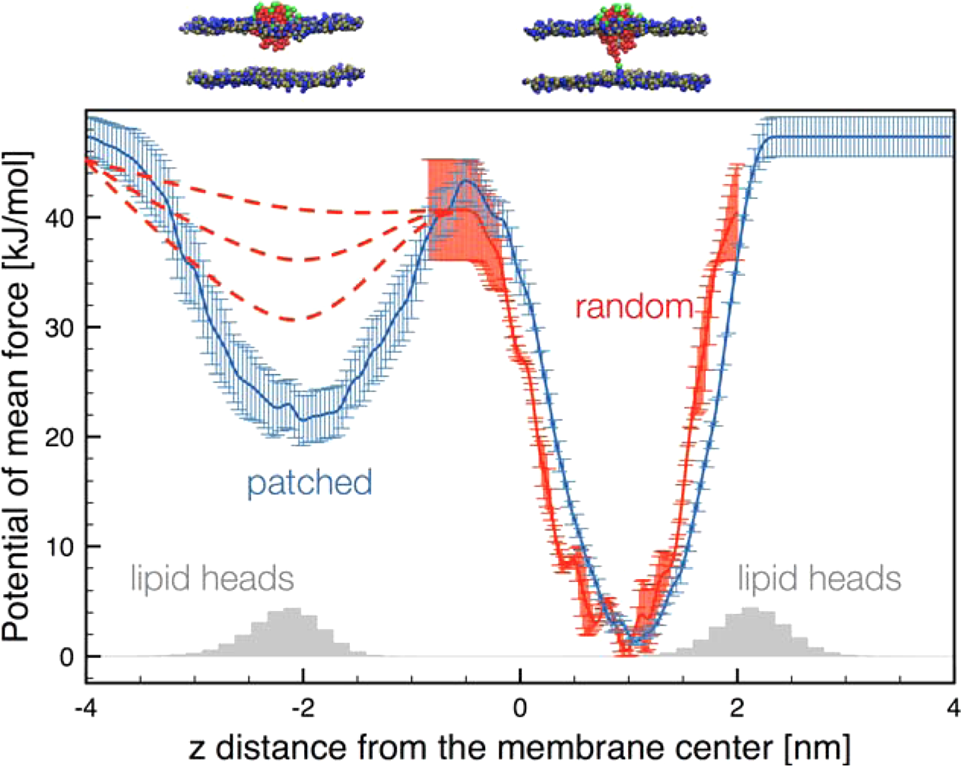
\includegraphics[width=0.7\textwidth]{./img/NPFES}
	\caption{Free energy profile related to the transfer of a negatively charged ligand from the entrance leaflet to the opposite one. The blue is related to the striped (\ac{MUS}:\ac{OT} $1$:$1$) configuration while the red to the random (\ac{MUS}:\ac{OT} $1$:$1$) configuration. Metadynamics data are shown with errorbars, while the red dashed line are hypothesized profiles for the stage $2$ to stage $3$ transition of random \acp{NP}. Gray shades show the position of the polar head beads (AU). Taken from \cite{ourPaper}.}
	\label{fig:NPFES}
\end{figure}
For the striped arrangement, the crossing barrier to reach the saddle point, located at $0.5$~nm off the \ac{COM} of \ac{POPC}, is of the order of $\sim 22$~kJ/mol. While the recrossing energy barrier is approximately twice as high. The same is for the recrossing barrier of the random configuration. The absent of data for the random \acp{NP} in the hydrophobic contact is due to the difficulty to sample the stage $2$ to the anchor state transition for only one charged ligand. This is because, while the metadynamics is running on a specific charged ligand, other charged ligands spontaneously anchor to the opposite leaflet, making the free energy sampling of the first anchor impossible. Hence, together with the kinematic, for which the average lifetime of stage $2$ for random \acp{NP} is three order of magnitude shorter than for striped, the authors confirm the very low energy barrier, of the order of few $k_B T$, for the anchor process of the random \acp{NP}.






 %MD tools, parallelization and hardware acceleration

% !TEX root = ./../main.tex
\chapter{Model of cell membrane and monolayer--protected NP}
\label{chap:membraneNP}
In the first part of this chapter we will present and describe the model of the charged monolayer--protected 
\ac{AuNP} developed by Federica Simonelli and co--workers in \cite{simonelliThesis} and \cite{ourPaper}. The gold 
core is treated by an all--atom representation, while the ligands are modeled at \ac{CG} level by the \martini 
\ac{FF}. In the second part of the chapter we will describe the most important physical and chemical features of 
the cell membrane. Then we will summarize the characteristics of the \ac{CG} model used to treat it. Finally, we 
will describe the \ac{NP}--biomembrane interaction mechanism and some preliminary thermodynamic results about the interaction of the 
\ac{AuNP} and the model cell membrane, as outlined in \cite{ourPaper}. For a more precise discussion about the 
\ac{NP}--membrane interaction and the models parameterization the reader is addressed to the work of Federica 
Simonelli \etal \cite{ourPaper} and her thesis work \cite{simonelliThesis}. For more details about the gold core used, its properties, equilibrium structure and so forth, the reader is addressed to the work of Lopez-Acevedo \etal \cite{clusterEquilibrium} while for a general discussion about thiolated \acp{AuNP} to the work of Häkkinen \cite{corePassivated}. For what concerns cell membranes and biological lipids the reader is addressed to the book by Yeagle \cite{yeagle}.

\section{NanoParticle model}
% gold core --> Thiol passivated --> ligands
%Ligand Composition: Patched (1:1), Random (1:1) (1:2)
%Different level of hydrophobicity
%Different ligand charge: anionic/cationic NP
Thiolated \acp{AuNP} in the $2-4$~nm range have a well defined molecular structure. That is, 
mono--dispersed solutions can be synthesized and structurally determined. Monolayer--protected 
\acp{AuNP} have a definite mass and molecular composition, and their structure is stabilized by the covalently 
bound ligands shell. \acp{AuNP} are biocompatible, have a facile surface chemistry and efficiently convert light into heat. Ligands are often thiols, as they covalently bind to the gold \ac{NP} by Au--S surface bonds, that is a robust but modifiable interaction, crucial in stabilizing the \ac{NP} and transmitting electronic interactions between gold and sulfur--containing organic molecules \cite{corePassivated}. Subtle changes of size, structure and 
ligand compositions and arrangements, can affect \ac{NP} properties such as their optical properties, important 
for biological sensing and therapeutics. Several stable thiolated \acp{AuNP} have been identified, differing in size of the gold core and number of ligands 
\cite{corePassivated}. In this thesis work we will consider the {Au$_{144}$(SR)$_{60}$} thiolated \ac{AuNP}, where 
R are the aliphatic chains of the thiol compounds. The equilibrium structure of the gold core were predicated by 
\textit{ab--initio} calculations in \cite{clusterEquilibrium}. 
%To overcome the computational cost of an atomistic model we use a \martini \ac{CG} model of the \ac{OT} and \ac{MUS} ligands. 

%The model of the \ac{AuNP} and the \martini model of the \ac{OT} and \ac{MUS} ligands are developed by Federica Simonelli \etal in \cite{ourPaper}, and the reader is addressed to it for a more detail discussion about the model and the parameterization.

\subsection{Passivated gold core}
% some information about gold core: dimensions, number of atoms, model used, elastic network, shel construction
The gold core is composed of $144$ atoms, it has icosahedral symmetry and it is made of three bulk shells with 
$12$, $42$ and $60$ atoms, respectively. A surface shell of $30$ atoms completes the gold cluster structure. Then 
$60$ sulfur atoms, which bind the aliphatic chains (R) to the gold core, are bounded to the gold atoms on the 
surface through the typical bond structure RS--Au--SR. The shell construction is shown in 
figure~(\ref{fig:goldShell}).
\begin{figure}[!ht]
	\centering
	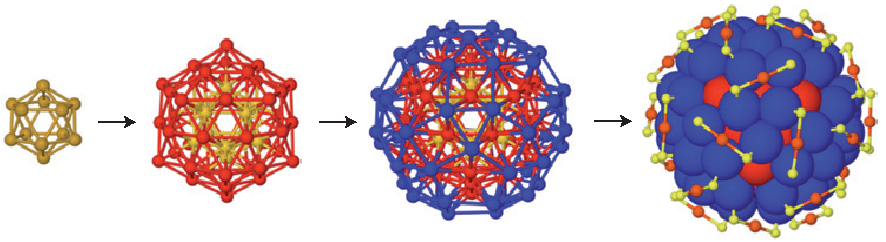
\includegraphics[width=0.8\textwidth]{./img/goldShell}
	\caption{First three frames: the concentric $12$--(yellow), $42$--(red) and $60$--(blue) atom gold internal shell, surrounded (last frame) by $30$ gold (red small) and $60$ sulfur (yellow small) surface atoms. The R chains are not shown. Taken from \cite{corePassivated}.}
	\label{fig:goldShell}
\end{figure}

The resulting diameter of the gold core is about $2$~nm. When passivated by thiols, its overall size depends on 
the length of the aliphatic chains bound to the sulfur atoms. The monolayer--protected \acp{AuNP} we will 
consider have a total diameter of about $4$~nm.

Despite the computational cost associated to atomistically describe the \ac{NP} core, all gold and sulfur atoms 
are taken into account. As shown in figure~(\ref{fig:coreNetwork}), bonds between gold and sulfur atoms are described with an elastic network potential of the form
\begin{equation*}
	U = \frac{1}{2}\sum_i \sideset{}{'}\sum_{j\ne i}k_{ij}(r_{ij} - r_{ij}^0)^2
\end{equation*}
where $r_{ij}$ is the distance, $k_{ij}$ is the bond constant for $i-j$ atom pair and the prime indicates that 
only neighbor atoms within a certain cutoff are considered. Thus, the atoms of the \ac{NP} core are allowed to vibrate.
\begin{figure}[h!t]
	\centering%
	\subfloat[Gold elastic network]{%
		\includegraphics[width=0.35\textwidth]{./img/goldNetwork}%
	}\qquad%
	\subfloat[\acs{AuNP} cluter]{%
		\includegraphics[width=0.32\textwidth]{./img/NPCluster}%
	}
	\caption{Left: gold elastic network. In cyan a surface atom and its neighbors; in blue bulk atom and its neighbors. Right: \acs{AuNP} cluster. The elastic network for both gold and sulfur atoms are represented by sticks. Taken from \cite{simonelliThesis} and \cite{ourPaper}.}
	\label{fig:coreNetwork}
\end{figure}

%The bond constants is assigned so as to reproduce the vibrational spectrum of the gold core as provided by the many--body Gupta potential. 
The bond constant is assigned to $k = 32500$~kJ/(mol\,nm$^2$) for Au--Au surface atoms, $k = 11000$ kJ/(mol\ 
nm$^2$) for Au--Au bulk atoms, $k = 1250$~kJ/(mol\,nm$^2$) for S--S atoms and $k = 32500$~kJ/(mol\,nm$^2$) for 
Au--S bonds, as summarized in table~(\ref{tab:NPConstants}). Instead, the equilibrium distances are derived from 
\textit{ab--initio} data in \cite{clusterEquilibrium}. Moreover, to prevent the penetration of other particles 
inside the \ac{NP} core, a purely repulsive interaction of the form $C/r^{-12}$ where 
$C = 0.92953\cdot 10^{-6}$~(kJ\,nm$^{12}$)/mol, is added between gold and sulfur atoms, gold and all other 
particles and sulfur and all other particles. A gold atom is considered as bulk atom if it has at least nine gold 
atom neighbors otherwise as a surface atom. Two gold atoms $i$ and $j$ are neighbors if their distance is 
$r_{ij} \le 0.35$~nm. Instead, two sulfur atoms are considered neighbors if they lie in a sphere shell of radius 
$0.55$~nm, i.e. each sulfur atom has at least five neighbors.
\begin{table}[h!t]
	\centering
	\begin{tabular}{lr}
		\toprule
		Bond			 & $k$\,\footnotesize[kJ/(mol\,nm$^2$)] \\ \toprule
		Au--Au (bulk) 	 & $11000$ 	\\ \midrule
		Au--Au (surface) & $32500$ 	\\ \midrule
		Au--S			 & $32500$ 	\\ \midrule
		S--S			 & $1250$ 	\\ \bottomrule
	\end{tabular}
	\caption{Summary of the bond constants for the elastic network of the \acs{NP} core.}
	\label{tab:NPConstants}
\end{table}

\subsection{Functionalizing ligands}
Changing the composition of the aliphatic chains bonded to the thiol group, different properties of the thiolated 
\ac{AuNP} can be achieved, such as different net charge, different level of hydrophobicity, different size and so 
on. In particular, our \ac{AuNP} core is functionalized with a monolayer of \ac{MUS} and \ac{OT} ligands with 
different compositions and surface arrangements, as shown in figure~(\ref{fig:figands}). \ac{MUS} is a charged 
compound made of an alkyl chain (\acs{CH2})$_{11}$ and a charged terminal \acs{SO4-} group. The charged terminal 
group makes \ac{MUS} partially hydrophilic. \ac{OT}, instead, is completely hydrophobic and it is made by an alkyl 
chain (\acs{CH2})$_{7}$ and one \acs{CH3} terminal group. Using both hydrophilic and hydrophobic groups guarantees 
that \acp{NP} are stable, that is, they do not aggregate in aqueous environments.
\begin{figure}[!ht]
	\centering
	\subfloat[\acs{OT} ligand]{%
		\includegraphics[width=0.3\textwidth]{./img/OT/OT}%
		\label{fig:ot}%
	}%
	\qquad\qquad%
	\subfloat[\acs{MUS} ligand]{%
		\includegraphics[width=0.35\textwidth]{./img/MUS/MUS}%
		\label{fig:mus}%
	}%
	\caption{Top: chemical structure. Bottom: \acs{CG} \martini model (red: C$_1$ bead, green: Qda negatively charged bead and yellow: sulfur atom).}
	\label{fig:figands}
\end{figure}

\paragraph{\textbf{OT Model}} Two \martini beads of type C$_1$ model the eight carbon atoms of the \ac{OT} 
backbone and their hydrogen atoms. The chemical structure and the resulting \ac{CG} \martini model is shown in 
figure~(\ref{fig:ot}). The first bead of each \ac{OT} ligand is bound to a sulfur atom via a harmonic potential 
with a bond constant of $1250$~kJ/(mol\,nm$^2$) and equilibrium length of $0.47$~nm. The second bead is connected 
to the first by the same bond potential. An angle potential as in equation~\eqref{eq:martiniAngle} is used among 
the three particles. Parameters are fixed in accordance with the \ac{STD} \martini parameters for alkanes. 
%Moreover a purely repulsive potential, as described previously, is used between C$_1$ beads and gold and sulfur 
%atoms to prevent the penetration of the \ac{NP} core.

\paragraph{\textbf{MUS Model}} Three \martini beads of type C$_1$ model the hydrophobic chain of the \ac{MUS} 
ligand. The charged group is modeled as a Qda bead with a charge of $-\mathsf{e}$. The chemical structure and the 
resulting \ac{CG} \martini model is shown in figure~(\ref{fig:mus}). Even in this case the first bead of a 
\ac{MUS} ligand is bound to the sulfur atom through a harmonic potential with the same parameter: bond constant 
of $1250$~kJ/(mol\,nm$^2$) and equilibrium length of $0.47$~nm. The same potential is used to bind all other 
beads to the previous one. An angle potential as in equation~\eqref{eq:martiniAngle} is used among the sulfur 
atom, the first C$_1$ and second C$_1$, among the first, the second and the third C$_1$ beads and so on for all 
four beads. Parameters are fixed in accordance with the \ac{STD} \martini parameters for alkanes.
%As in the \ac{OT} ligand 
%model, a purely repulsive potential, as described previously, is used between C$_1$ beads and gold and sulfur 
%atoms to prevent the \ac{NP} penetration. The same applies between Qda bead and gold and sulfur atoms.

\paragraph{\textbf{level of hydrophobicity}} The \ac{AuNP} core can be functionalized with both ligands at 
different composition. In particular varying the ratio between the \ac{OT} and \ac{MUS} ligands different levels 
of hydrophobicity can be reached. Two surface compositions will be considered in this thesis work: 
(\ac{MUS}:\ac{OT} $1$:$1$) and (2:1), the former is the main used in this thesis work. This choice is due to the 
possibility to compare to previous experimental and simulation data \cite{Maccarini2013}, \cite{VanLehn2013}, 
\cite{VanLehn2014} and \cite{VanLehn2015}.

\paragraph{\textbf{surface arrangements}} The ligands on the \ac{AuNP} surface can be arranged in two possible 
ways: randomly or with a predetermined scheme. We will consider both \acp{NP} with a random ligand arrangement 
and \acp{NP} with a striped ligand arrangement. The striped scheme is obtained dividing the \ac{NP} surface in 
three stripes: the external two stripes are covered with \ac{MUS} ligands while the central with \ac{OT} ligands. 
For this thesis work we consider three type of \acp{NP}: striped (\ac{MUS}:\ac{OT} $1$:$1$), random 
(\ac{MUS}:\ac{OT} $1$:$1$) and random (\ac{MUS}:\ac{OT} $2$:$1$). In figure~(\ref{fig:coating}) three different 
coatings are shown.

\begin{figure}[!ht]
	\centering
	\subfloat[striped ($1$:$1$)]{
		\includegraphics[width=3.3cm]{./img/coatings/striped}
	}%
	\qquad
	\subfloat[random ($1$:$1$)]{
		\includegraphics[width=2.9cm]{./img/coatings/random11}
	}%
	\qquad
	\subfloat[random ($2$:$1$)]{
		\includegraphics[width=2.7cm]{./img/coatings/random21}
	}%
	\caption{Au\acs{NP} with different ligand surface arrangements and composition. From left to right: striped (\ac{MUS}:\ac{OT} $1$:$1$), random (\ac{MUS}:\ac{OT} $1$:$1$) and random (\ac{MUS}:\ac{OT} $2$:$1$). Hydrophobic beads are shown in red while the negatively charged beads are green.}
	\label{fig:coating}
\end{figure}

\section{Cell membranes}
%The cell membrane or cytoplasmic membrane is a biological membrane that separates the internal and the external environments of a living cell and controls communications and nutrient flow in and out of the cell. This is essential to enable the functions of cells. The membrane main function is the compartmentalization of a biological environment into two well defined, though not independent, subsections: the cell in which the ``life reactions'' take place and the external cell fluid in which all the necessary biological compounds are dissolved. The compartmentalization in such environments enhance the probability of chemical reactions to take place inside the cells but also allow to develop different chemical reactions inside and outside the cells. From an evolutionary point of view it is believed that a simple membrane that defines an inside and an outside environments and that protect and concentrates molecules in a closed space, it was necessary for the development of life.
The cell membrane or cytoplasmic membrane is a biological membrane whose main function is to compartmentalize the biological environment into two well defined, though not independent, subsections: the interior of the cell and its external environment. The membrane controls the in--out flow of ions and other chemical compounds which are necessary to carry out all ``life reactions'' taking place inside the cell. For these reasons it is believed that the appearance of a simple membrane that defines an inside and an outside environment and that protects and concentrates molecules in a closed space, was necessary for the development of life.

\subsection{Real cell membranes}
Since the compartmentalization, the cell membrane have to allow the exchange of biological molecules from and to the outside world. This role is, in a small part, fulfilled by the membrane itself through the passive translocation of small molecules or ions. But the main part is fulfilled through proteins and other compounds that are solved inside the membrane. As we can see from a cartoon of a real cell membrane in figure~(\ref{fig:cellMembrane}), the biological membrane is a crowded environment consisting of phospholipids, glycolipids, carbohydrates, proteins and other organic molecules.
\begin{figure}[!ht]
	\centering
	\includegraphics[width=0.9\textwidth]{./img/cellMembrane}
	\caption{Schematic representation of a biological cell membrane.}
	\label{fig:cellMembrane}
\end{figure}

The plasma membrane by mass is essentially composed by half lipids and half proteins. The lipids that constitute the membrane are a particular type of lipids, called \textit{phospholipids}. They are made of a neutral (polar) or charged head, which is hydrophilic and one or two fatty acid hydrocarbon chains, often called lipid tails, which are instead hydrophobic, as shown schematically to the left of figure~(\ref{fig:phospho}). Due to have both properties a phospholipid is an \textit{amphiphilic} molecule. This amphiphilic nature, through the \textit{hydrophobic effect}, play a key role in the membrane formation. In fact when we put a relevant concentration of phospholipids in a water solution at a certain temperature, the lipid tails tend to move away from water molecules due to the hydrophobic effect, so they tend to get closer between them in order to minimize the hydrophobic surface in contact with water. Instead, the polar heads tend to make favorable bonds with water molecules. The resultant bilayer configuration, proper of the biological membrane, is shown schematically to the right of figure~(\ref{fig:phospho}). 
\begin{figure}[!ht]
	\centering
	\includegraphics[width=0.6\textwidth]{./img/phospholipids}
	\caption{Left: schematic representation of a phospholipid. Right: self--assembled bilayer configuration assumed by an aqueous solution of phospholipids.}
	\label{fig:phospho}
\end{figure}
Hence, the phospholipids in a water solution tend to \textit{spontaneously} self--organize in a \textit{ordered} state that minimize the Gibbs free energy and that depends on the lipids concentration and the temperature of the solution. As schematically shown in figure~(\ref{fig:lipidsStructures}) the final configurations of such self--assembly process are essentially three: the bilayer sheet, a liposome and a micelle.
\begin{SCfigure}[][!ht]
	\centering
	\includegraphics[width=0.35\textwidth]{./img/lipidsStructures}
	\caption{Cross--sectional view of the structures that can be formed by a self--assembly process of a phospholipid aqueous solution.}
	\label{fig:lipidsStructures}
\end{SCfigure}

A real lipid bilayer often contains hundred of different lipid species. They differ in the length of the 
hydrocarbon chains, in the degree of unsaturation, i.e. in the number of double bond in the hydrocarbon chains, 
and in different composition of the head that can be neutral (polar) or charged. There are two main classes of 
phospholipids that make a cell membrane of animals: glycerophospholipid (phosphatidyl--choline, 
phophatidyl--ethanolamine, phophatidyl--serine, phosphatidyl--serine ) and phosphosphingolipids (sphingomyelin). 
In the former group the lipid tails are bound to a glycerol group while the latter do not have glycerol and the 
lipid tails have a backbone of sphingoid bases, absent in the former. These five types take into account for more 
then half of the lipids in most membranes.

The cell membrane has quasi--liquid properties at physiological temperature. This is in part due to some disorder 
in the alignment of the lipid tails produced by the presence of unsaturated chains. Another contribution arise 
from the area occupied by the lipid heads which determines the distance between the hydrocarbon chains. This 
fluid character makes the lipid bilayer like a solvent in which the other molecules (lipids and proteins) are 
dissolved and are free to diffuse. Moreover the lipids itself can move in different ways. The main movements and 
the associated time scales are summarized as follow
\begin{itemize}
	\item lipids conformational change (few nanoseconds);
	\item lipids protrusions out--of--plane (tens of picoseconds);
	\item diffusion within a leaflet (order of tens of nanoseconds);
	\item bilayer undulation and thickness involving collective motion of many lipids (order greater than tens of microseconds).%
\end{itemize}
There are also many rare events that take place on the order of hours or even days, such as lipid flip--flop, in 
which a lipid flips from one leaflet to the opposite one; ion translocation; \textit{electroporation} by water, 
for example due to a cross membrane ion imbalance, in which water translocates across the bilayer; water assisted 
ion permeation via formation of a \textit{water--finger} and so forth.

For what concerns the length scales, the bilayer thickness is determined by the length of the lipid tails and 
their degree of unsaturation. Typically the hydrophobic region is $\sim 3$~nm thick while each hydrophilic 
region is $\sim 1$~nm thick. Hence the typical bilayer thickness is around $\sim 4\div 5$~nm.

\subsection{Model cell membrane}
As we have seen above, the cell membrane is an extremely complex environment due to the large number of different biological molecules (lipids, proteins and so on) which compose and reside in the membrane. The model membranes we will consider in this thesis will be composed of lipids only. This choice is dictated by three main reasons. First, current models and computational power can not aim at reproducing the complexity of a real plasma membrane. Second, the use of a model system allows to tackle fundamental questions concerning the physical and molecular mechanisms of interaction between \acp{NP} and membranes. Last but not least, the model membrane we will consider resembles closely the model membranes used in a number of experimental and simulations results.  

In the bilayer model we will use, we consider a model biological membrane consisting of \ac{POPC} lipids; the 
chemical structure is shown in the top of figure~(\ref{fig:popc}). It is a zwitterionic glycerophospholipid of 
type phosphatidyl--choline whose head is made of a phosphate (PO$_4^-$) and a choline (C$_5$H$_{14}$NO$^+$) 
groups. It has two hydrocarbon chains: one is a saturated chain (palmitoyl) and the other is an unsaturated chain 
(oleoyl). The head groups and tails are both bounded to the glycerol group (C$_3$H$_8$O$_3$).
\begin{figure}[!ht]
	\centering
	\includegraphics[width=0.7\textwidth]{./img/POPC/popc}
	\caption{Top: chemical structure of a \acs{POPC} lipid. Bottom: \martini \acs{CG} model. The tan bead is the phosphate group, choline is in blue, the two pink beads represent the glycerol group and the hydrophobic chains in cyan.}
	\label{fig:popc}
\end{figure}

\paragraph{\textbf{CG model}} It is clear that the number of lipids that constitute a real cell membrane is 
enormous and it is impossible to take into account an entire cell membrane in a \ac{MD} simulation. A first 
approximation is to consider only a small area of the model bilayer. Given the medium area per lipid of about 
$0.65$~nm$^2$ and a portion of bilayer of $\sim 160$~nm$^2$, which corresponds to about $250$ lipids per leaflet, 
the total number of particles to be included in a atomistic simulation (excluding hydrogen atoms) are about 
$26\cdot 10^3$ plus the water molecules ($\sim 7\cdot 10^4$). This has a very expensive computational cost and 
the range of phenomena which can be studied on these time and length scales are very limited, calling for the 
adoption of a \ac{CG} approach.

\paragraph{\textbf{martini model}} As described in section \ref{sec:martini}, we will use the 
\ac{CG} \martini \ac{FF} for lipids \cite{Martini}.
%We consider a lipid bilayer made of $512$ \ac{POPC} lipids which extend on a surface of about $160$~nm$^2$ and whose thickness is about $4$~nm. 
The \martini model for the \ac{POPC} lipid maps the choline and the phosphate groups into two beads of type Q$_0$ 
and Qa negatively and positively charged, respectively. The saturated tail is modeled with four beads of type 
C$_1$ while the unsaturated tail is built up of four C$_1$ beads and one C$3$ bead that corresponds to the 
unsaturated group of atoms. The glycerol group is modeled with two beads of type N$_\text{a}$. A comparison 
between the chemical structure and \ac{CG} model is shown in figure~(\ref{fig:popc}).

\paragraph{\textbf{model accuracy}} The \ac{STD} \martini \ac{FF} is able to capture the main physical properties 
of a lipid bilayer. These properties include the area per lipid, the distribution of groups across the membrane, 
the trend of the bending and the area compression moduli in function of the lipid composition and the 
unsaturation degree of the lipids, the stress profile across the membrane, and many other as better described in 
\cite{Martini} and \cite{MartiniReview}. Some of the main properties of a pure \ac{POPC} bilayer are shown in 
table~(\ref{tab:POPCData}) in a comparison with different models. Nevertheless many other properties, prevalently mediated by the electrostatic interaction, are not well described. As we have seen in chapter~\ref{chap:EmpiricalFF}, this is because the \ac{STD} \martini \ac{FF} does not take into account the long range treatment of the electrostatic interaction. To overcome this problem the use of the \ac{PME} method and the \ac{PW} model, as outlined in sections~\ref{sec:electrostaticInt} and~\ref{sec:pw}, are crucial to better describe the processes that involve the interaction between ions, water and lipid bilayer. These are ion translocation; electroporation of the membrane by water, due to a cross membrane ion imbalance; water--helped ion permeation and many other water defects inside the membrane as better described in the works of Marrink \cite{MartiniReview} and Yesylevskyy \cite{PW}. 
\begin{table}[h!t]
	\centering
	\begin{tabular}{lcccc}
		\toprule
		\,				& STD$^a$	& \acs{PME}$^b$	& \acs{PME} + \acs{PW}$^b$	& atomistic$^c$ \\ \toprule
		$D$	[$10^{-8}$~cm$^2$/s]	& $\sim62$	& $43.3 \pm 0.7$ & $31 \pm 1$	& $8.0 \pm 0.4$	\\ \midrule
		$\overline{A}$ [nm$^2$]		& $0.65$	& $0.630$		 & $0.635$		& $0.688$		\\ \midrule
		$\overline{t}$ [nm]			& $4.16$	& $4.29$		 & $4.26$ 		& $3.66$		\\ \bottomrule
	\end{tabular}
	\caption{Summary of main properties of a pure \acs{POPC} bilayer in comparison with different models. $D$ is the lateral diffusion coefficient of a lipid. $\overline{A}$ is the average area per lipid. $\overline{t}$ is the bilayer thickness as the average distance of the phosphate groups. \footnotesize $^a$ Data from \cite{Rossi2014}. $^b$ Data obtained from my \ac{MD} runs. $^c$ Data courtesy of Federica Simonelli.}
	\label{tab:POPCData}
\end{table}

\newpage
\section{NP--Membrane interaction}
\label{sec:NPMembraneInt}
Recently the literature concerning the computational modeling about the interaction of anionic 
monolayer--protected \ac{AuNP} and model lipid membranes has expanded contributing to sketch a possible mechanism 
of such interaction. The first step of the interaction between the \ac{NP}, dissolved in the extracellular 
water environment, and the membrane is the attraction between the charged ligands and the polar head of the 
zwitterionic phospholipids: electrostatics it is recognized to be the driving force for the adhesion of the 
\ac{AuNP} to the membrane surface, figure~(\ref{fig:threeProcess}a). To the other end of the pathway, it is 
predicted, on thermodynamic basis, that the most stable state for the \ac{AuNP} corresponds to the so--called 
\textit{snorkeling} configuration in which the \ac{NP} is embedded in the hydrophobic region of the membrane, 
while the charged ligands stably interact with the lipid heads of both leaflets, 
figure~(\ref{fig:threeProcess}f). 

In the work of Federica Simonelli \etal \cite{ourPaper}, using the \ac{STD} \martini \ac{FF}, the authors found 
and characterized a possible mechanism of the interaction process, as better detailed in the next paragraph. In 
the next paragraph we summarize the findings of Simonelli \etal, which constitute the starting point of the 
development of my thesis work.

\subsection{Three--stage process}
%\paragraph{\textbf{Three--stage process}} 
The authors found a three--stage mechanism that regulates the insertion of the \ac{AuNP} into the core of a planar membrane: from the adsorbed state, figure~(\ref{fig:threeProcess}a), to the snorkeling configuration, 
figure~(\ref{fig:threeProcess}f). When the \ac{NP} in the water phase is approaching the surface of the membrane 
it enters in the stage $1$, the adsorbed state, in which the charged ligands interact with the polar lipid heads. 
The stage $2$ is the hydrophobic contact, figure~(\ref{fig:threeProcess}d), in which the hydrophobic beads of the 
\ac{MUS} and \ac{OT} ligands are in contact with the hydrophobic tails of the membrane while the charged bead of 
the \ac{MUS} ligands are still in the water phase or in contact with the lipid heads. The stage $3$ is the 
snorkeling configuration, figure~(\ref{fig:threeProcess}f). 

A key role for the transition stage $1$ to stage $2$ transition is played by a lipid tail protrusion out of the hydrophobic region that stably interacts with the hydrophobic beads of the \ac{NP} ligands, 
figure~(\ref{fig:threeProcess}b\,-\,c). The protruding lipid pulls the \ac{OT} ligands into the membrane core and the \ac{NP} enter the hydrophobic state, figure~(\ref{fig:threeProcess}d). The lipid tail protrusion mechanism is validated by the kinematic of the simulations: the energy barrier to be overcome to move from stage $1$ to stage $2$ is of the order of the estimated energy cost of a lipid tail protrusion \cite{VanLehn2015}. Subsequently due to thermal fluctuations a charged bead can cross the membrane core and stably interact with the head region of the opposite leaflet bringing the \ac{NP} in the anchored state, figure~(\ref{fig:threeProcess}e).
\begin{figure}[t]
	\centering
	\subfloat[]{
		\includegraphics[width=4cm]{./img/threeProcess/a}
	}%
	\quad%
	\subfloat[]{
		\includegraphics[width=4cm]{./img/threeProcess/b}
	}%
	\quad%
	\subfloat[]{
		\includegraphics[width=4cm]{./img/threeProcess/c}
	}%
	\\%
	\subfloat[]{
		\includegraphics[width=4cm]{./img/threeProcess/d}
	}
	\subfloat[]{
		\includegraphics[width=4cm]{./img/threeProcess/e}
	}%
	\quad%
	\subfloat[]{
		\includegraphics[width=4cm]{./img/threeProcess/f}
	}%
	\caption{\acs{AuNP}--membrane interaction. (a) stage $1$, adsorption of the \acs{NP} at membrane surface; (b) to (d) stage $2$, the protrusion of a lipid tail initiates the hydrophobic contact that leads to partial embedding of the \acs{NP} in the membrane core; (e) the \ac{NP} binds to the opposite leaflet throwing a charged ligand; (f), stage $3$, snorkeling configuration (five anchors shown). The hydrophobic beads of the ligands are shown in red and the charged beads in green. Lipid heads are blue (choline) and tan (phosphate), lipid tails are not shown, expect for (b) and (c), where the protruding lipid is shown with yellow tails. Water beads are not shown. All snapshot refer to a random (\ac{MUS}:\ac{OT} $1$:$1$) configuration. Taken from \cite{ourPaper}.}
	\label{fig:threeProcess}
\end{figure}
According to the \ac{STD} \martini model, the anchored state is thermodynamically favorable with respect to the hydrophobic state. Indeed, in the unbiased \ac{MD} simulations performed by Simonelli \etal, after the first anchor had been dropped, more and more ligands would anchor to the head region of the opposite leaflet, approaching step--by--step the snorkeling configuration, figure~(\ref{fig:threeProcess}f). Eventually, and consistently with previous thermodynamics--based models [], Simonelli \etal found that the energy cost associated with the extraction of the \ac{NP} out of the membrane core is very high, making the anchoring process, and the snorkeling configuration, almost irreversible. We want to stress out that all the aforementioned transitions 
are triggered by rare molecular events: the lipid tail protrusion and the membrane translocation of a charged 
bead. Hence they could be observed to happen spontaneously only thanks to the use of a \ac{CG} \ac{FF}. 
 
Simonelli \etal performed \ac{MD} simulations for the three different \ac{NP} configurations showed in 
figure~(\ref{fig:coating}): the striped (\ac{MUS}:\ac{OT} $1$:$1$), the random (\ac{MUS}:\ac{OT} $1$:$1$) and the 
random (\ac{MUS}:\ac{OT} $2$:$1$). They found that the described behavior is common to the three configurations.  
Nevertheless, after the hydrophobic contact is reached, its lifetime depends on the surface ligand arrangement. 
For the random configurations the time lag between the hydrophobic contact and the first anchor is on the order 
of few nanoseconds. Instead, the striped configuration can linger in the stage $2$ for several microseconds. This 
suggest that the energy barrier to be overcome to move from stage $2$ to the anchored state is lower for the 
former than that for the latter. 

\subsection{Preliminary metadynamics results}
\label{sec:preliminaryMetadyn}
To quantify the thermodynamic behavior, Simonelli \etal performed metadynamics calculations. In particular, in 
order to estimate the energy barrier for the anchoring process, metadynamics was used to enhance the sampling of 
the transition of the first anchoring ligand from the entrance leaflet to the opposite one. The metadynamics bias potential was applied to the $z$ component of the distance between the center of one charged ligand terminal and the \ac{COM} of the \ac{POPC} bilayer, as shown in figure~(\ref{fig:CVRappresentation}). This distance is thus the \ac{CV}.
\begin{figure}[ht!]
	\center
	\includegraphics[width=0.7\textwidth]{./img/CV/CV}
	\caption{Schematic representation of the chosen \acs{CV} and the bias potential deposition along the \acs{CV} space. The thicker dashed line is the center of the bilayer.}
	\label{fig:CVRappresentation}
\end{figure}

The convergence of such a run is achieved when the charged bead is able to freely diffuse across 
the membrane. As the size and the complexity of the system does not allow to achieve the convergence, not even at 
\ac{CG} level, the authors decided to perform different statistically independent metadynamics runs and stop each 
simulation at the recrossing process of the biased ligand. A recrossing is determined when, after the anchoring has taken place, the charged bead returns towards the entrance leaflet. The transition back to the hydrophobic state typically require the ligand to reach $z=-0.5$~nm on the way back. The resulting \ac{FES} profile, shown in 
figure~(\ref{fig:NPFES}), is obtained averaging the statistically independent runs. The error bars are the 
standard error of the independent runs, as described in \ref{sec:metadynamics}.
\begin{SCfigure}[][!b]
	\includegraphics[width=0.6\textwidth]{./img/NPFES}
	\caption{Free energy profile related to the transfer of a negatively charged ligand from the entrance leaflet to the opposite one. The blue is related to the striped (\ac{MUS}:\ac{OT} $1$:$1$) configuration while the red to the random (\ac{MUS}:\ac{OT} $1$:$1$) configuration. Metadynamics data are shown with error bars, while the red dashed line are hypothesized profiles for the stage $2$ to stage $3$ transition of random \acp{NP}. Gray shades show the position of the polar head beads (AU). Taken from \cite{ourPaper}.}
	\label{fig:NPFES}
\end{SCfigure}

For the striped arrangement, the crossing barrier to reach the saddle point, located at $0.5$~nm off the \ac{COM} 
of \ac{POPC}, is of the order of $\sim 22$~kJ/mol. While the recrossing energy barrier is approximately twice as 
high. The same is for the recrossing barrier of the random configuration. The absence of data for the random 
\acp{NP} in the hydrophobic contact is due to the difficulty to sample the stage $2$, whose lifetime is too short 
(few nanoseconds).

%to the anchor state transition for only one charged ligand. This is because, while the metadynamics is running on a specific charged ligand, other charged ligands spontaneously anchor to the opposite leaflet, making the free energy sampling of the first anchor impossible. Hence, together with the kinematic, for which the average lifetime of stage $2$ for random \acp{NP} is three order of magnitude shorter than for striped, the authors confirm the very low energy barrier, of the order of few $k_B T$, for the anchor process of the random \acp{NP}.
 %Model of cell membrane and monolayer--protected NP

% !TEX root = ./../main.tex
\chapter{Results}
\label{chap:results}
The results summarized in section~\ref{sec:NPMembraneInt} were obtained using the \ac{STD} \martini{} \ac{FF}, 
with a cut--off method for treating the electrostatic interactions. Unfortunately, as we have seen in 
chapter~\ref{chap:EmpiricalFF}, such method poorly describes the processes that involve the transfer of a charged 
moiety from a polar (e.g. water) environment to an non--polar one (e.g. the membrane core).

Our aim is thus to perform a comparison between the \ac{STD} \martini{} model and two versions of \martini{} that 
better take into account electrostatic interactions. We will consider
\begin{enumerate}[label=\itshape\roman*.]
	\item the \martini{} \ac{FF} with long range electrostatics (\martini{} + \ac{PME});
	\item the \martini{} \ac{FF} with long range electrostatics and \ac{PW} (\martini{} + \ac{PME}/\acs{PW}).
\end{enumerate}

In this chapter we present the main results of this thesis. In section~\ref{sec:resultsBiased} we calculate, using 
the metadynamics method, the free energy barrier for the \ac{NP} anchoring (and dis--anchoring) process using 
versions \textit{i}. and \textit{ii}. of the \martini{} \ac{FF}, and compare the outcomes to those obtained with 
the \ac{STD} \martini{} model and with atomistic simulations. The introduction of long--range electrostatics has 
the overall effect of increasing the energy barriers for the translocation of charged ligands.

In section~\ref{sec:resultsUnBiased} we focus on the description of the molecular processes that take place during the anchoring/dis--anchoring of the \ac{NP}. This analysis will be applied to both biased (metadynamics) trajectories and unbiased \ac{MD} runs, and it will allow to quantify the degree of alteration of the membrane structural properties during the interaction with the \ac{NP}.

% The pathway to improve the model is the use of the \ac{PME} method to better describe the electrostatic interaction and the use of the \ac{PW} model to improve the behavior of the water solvent at a \ac{CG} level. For a comparison to be made, the idea, is to follow the procedure describe in section~\ref{sec:preliminaryMetadyn} and, with metadynamics runs, try to estimate the energy barrier of the anchoring process with the use of the \ac{PME} alone and in combination with the \ac{PW} model.
%
% Preliminary, some tests about the use of the \ac{PME} method and the \ac{PW} model with a pure \ac{POPC} bilayer was performed. Then metadynamics runs for obtaining the \ac{FES} of the anchoring process involving both the striped (\ac{MUS}:\ac{OT} $1$:$1$) and the random (\ac{MUS}:\ac{OT} $1$:$1$) \acp{NP} were performed with the use of the \ac{PME} alone and in combination with the \ac{PW}.
%In view of the results, then, as better described in the next chapter, unbiased \ac{MD} runs with the use of \ac{PME} and \ac{PW} involving all the \ac{NP} configurations were performed in order to investigate a possible change in the kinematic of the all the \ac{NP}--membrane interaction process.

\section{Thermodynamic results}
\label{sec:resultsBiased}
The process that I will consider for the \ac{FES} estimation of the ligand anchoring is composed of two steps: the 
forward process: from the hydrophobic state to the state with one anchor; the backward process: from the anchored 
state to the hydrophobic state again.

\paragraph{\textbf{system set--up}} In all of my biased and unbiased \ac{MD} runs the membrane bilayer is made of 
$256$ \ac{POPC} lipids per leaflet. I will consider both the striped (\ac{MUS}:\ac{OT} $1$:$1$) and the random 
(\ac{MUS}:\ac{OT} $1$:$1$) \acp{NP}. The simulation box is neutralized with $30$ counteracting Na$^+$ 
ions\footnote{The \martini{} model for ions, especially for Na$^+$ and Cl$^-$, associates the ion plus the 
hydration shell to a bead of type Qd positively charged and Qa negatively charged, respectively.} and filled by 
water. In figure~(\ref{fig:startFrameHydro}) it is shown an example of the starting configuration for a striped 
(\ac{MUS}:\ac{OT} $1$:$1$) \ac{NP} in the hydrophobic state. The initial configuration frames with the \ac{PW} are 
obtained from the initial configuration frames with the \ac{STD} \martini{} water using a python script that 
converts the \ac{STD} \martini{} water to the \ac{PW} bead. With the \ac{PW} an equilibration run with the 
parameters shown in the third column of table~(\ref{tab:inputParam}) is necessary to stabilize the system. As 
already shown in figure~(\ref{fig:CVRappresentation}), our metadynamics runs use as \ac{CV} the distance between 
one single charged ligand terminal and the \ac{COM} of \ac{POPC} along the normal. The charged ligand for the 
anchoring process is chosen so as to be the lowest charged ligand attached to the \ac{NP} core. For what concerns 
the metadynamics input parameters used to perform my \ac{MD} runs, if not differently specified, they are 
summarized in table~(\ref{tab:metadynParam}).
\begin{SCfigure}[][!ht]
	\centering
	\includegraphics[width=0.42\textwidth]{./img/patchedHydrophobic.pdf}
	\caption{Example of a starting configuration of a metadynamics run of a striped (\ac{MUS}:\ac{OT} $1$:$1$) \ac{NP} in the hydrophobic state. Color code as in figure~(\ref{fig:threeProcess}). The charged ligand chosen for the anchoring process is in orange. The dashed line is the center of the bilayer. The blue contour is the simulation box. Water beads and lipid tails are not shown.}%
	\label{fig:startFrameHydro}
\end{SCfigure}

% \paragraph{\textbf{CV issues}} The \ac{CV} chosen to describe the anchoring process is the $z$ component of the distance between the center of the charged bead and the \ac{COM} of the bilayer. Although this \ac{CV} is a very intuitive and simple, with the introduction of the \ac{PME} method, and more accentuated with the \ac{PW} model, we found that it suffers of some issues. When I perform the metadynamics runs with the \ac{PME} and \ac{PW}, in accordance with the atomistic results, it is observed that the anchored state is more stable than with the \ac{STD} \martini{} models: the increase of the model accuracy make the interaction between the negatively charged bead and the positively charged choline group of the lipid heads of the opposite leaflet, stronger than with the \ac{STD} \martini{}. The same apply with the \ac{PW} beads. Hence, like in figure~(\ref{fig:engulfment}), we observe that when the metadynamics try to dis--anchor the charged bead in the backward process, it pull back the lipid heads slightly deforming the opposite leaflet of the bilayer. This results in a worse estimation of the \ac{CV} because the charged ligand is in the hydrophobic region near the entrance leaflet but still in contact with one or two lipid heads of the opposite leaflet.
% \begin{SCfigure}[][h!t]
% 	\centering
% 	\includegraphics[width=0.5\textwidth]{./img/patchedEngulfment}
% 	\caption{Detail of the engulfment effect in the anchoring leaflet when the ligand tends to dis--anchor. Color code as in figure~(\ref{fig:threeProcess}). Lipid tails are shown in cyan while the glycerol group is represented by the violet beads. Water and other lipid tails are not shown. The choline group (blue bead) is in contact with the charged bead of the ligand (pink beads) and the lipid tails are horizontal instead of vertical as they usually are.}
% 	\label{fig:engulfment}
% \end{SCfigure}
% Another import issue as the simulation time increase and related to the previous issues, is the loss of the ability by the \ac{CV} to well distinguish the two states, although the convergence has not yet reached. In figure~(\ref{fig:NPDist}) the red line is the \ac{CV}. In the region $z > 1$ the ligand have crossed the \ac{COM} of the bilayer and it is anchored in the opposite leaflet. For $z < -1$ the ligand is near the \ac{NP}'s leaflet in the hydrophobic state. While for $-1 < z < 1$ the ligand is in the hydrophobic region of the membrane but it may be in contact with the lipid head beads of the opposite leaflet. Hence inside the dashed black lines there is a region of the \ac{CV} space in which the two states are overlapping. This issue leads in a underestimation of the forward wall of the one anchor \ac{FES} because it tend to lower the saddle point while the metadynamics is still sampling the anchored state.
% \begin{figure}[!ht]
% 	\centering
% 	\includegraphics[width=0.7\textwidth]{./img/results/NPDistance/NPDist}
% 	\caption{Correlation between the \acs{CV} (red) and the $z$ component of the distance between the \acs{COM} of the \acs{NP} and the \acs{COM} of the bilayer (green) as a function of the simulation time. The region of the \acs{CV} space inside the dashed black lines is the overlapping region. Data obtained from a $6.5$~$\mu$s metadynamics run of a striped (\acs{MUS}:\acs{OT} $1$:$1$) \acs{NP} with \acs{PW}.}
% 	\label{fig:NPDist}
% \end{figure}
%
% %Moreover, since the interaction with the lipid heads is stronger,
%
% \paragraph{\textbf{convergence problems}} An important issue related to this process is the achievement of the convergence, essential in the \ac{FES} estimation. Our metadynamics runs have not reached the convergence, even in tens of microseconds of simulation, as we can see from figure~(\ref{fig:NPDist}) (red) of a $6.5$~$\mu$s test run in which we try to reach the convergence\footnote{In this run in an attempt to speed up the achievement of the convergence, in addition to the metadynamics bias, I use two other harmonic bias to limit the sampled region. Un upper bias which is activated when the charged bead is far from the bilayer \acs{COM} for more than $3$~nm and a lower bias when the charged bead is far from the bilayer \acs{COM} for more than $-4$~nm. The elastic constant is chosen $k = 100$~kJ/mol for both.}. This is prevalently due to the just described issues associated to the \ac{CV}. But also, in accordance with my unbiased simulations and the atomistic results, because the energy barriers associated to the two metastable state are much higher than what are estimated in \cite{ourPaper}, slowing down the reaching of the convergence. Another issues is related to stronger interaction between the charged bead and the \ac{PW} beads and the charged bead and the lipid heads. From the metadynamics runs, for the random and more pronounced for the striped \acp{NP}, we observe that, respect to the \ac{STD} \martini{} model, the charged ligand spend a not negligible time completely soaked in the water phase ($z>-2$). This leads to sample a region of the \ac{CV} space useless for one anchor \ac{FES} estimation and tend to slow down the achievement of the convergence. Another undesired process that we observe as the simulation time increase, is a small drag of the \ac{NP} inside the bilayer by the charged ligand in the anchored state. From figure~(\ref{fig:NPDist}), since the stronger interaction with water, we see that when the charged bead is approaching the water phase of the opposite leaflet ($z>2$) it is not only due to the ligand itself but also because the \ac{COM} of the \ac{NP} tend to approach the \ac{COM} of the bilayer (green). Despite this can be an important molecular process in order for a comparison to be made, we must not sample the phase phase associated to the movement of the \ac{COM} of the \ac{NP} since we are interested in the \ac{FES} associated to the anchoring process only.
%
% \paragraph{\textbf{worse estimation of the FES}} From the previous explanations it is clear that following the procedure outlined in \cite{ourPaper} leads to a worse estimation of the \ac{FES} associated to the anchoring process. In particular all these issues suggest a different pathway, at molecular level, for the forward process respect to the backward process and that some other \acp{CV} are missing. Hence, using the same \ac{CV}, instead to try to estimate the whole \ac{FES}, we can try to estimate the energy wall associated to the forward process and, separately, the energy wall associated to the backward process. For the estimation of the energy wall of the forward process we need to start the metadynamics runs in the hydrophobic state and stop it when the ligand reach the anchored state. For the backward process we need to do the contrary: start the metadynamics from the anchored state and stop it when the ligand return to \ac{NP} leaflet. Then we can compare the new results with the \ac{STD} \martini{} model and the atomistic one.
%la usiamo per stimare la barriera di andata e ritorno

\subsection{Forward process}
I have performed ten metadynamics runs starting from the hydrophobic state for each of the following 
``configurations'': striped (\ac{MUS}:\ac{OT} $1$:$1$) with \ac{PME}; striped (\ac{MUS}:\ac{OT} $1$:$1$) with 
\ac{PME} and \ac{PW}; random (\ac{MUS}:\ac{OT} $1$:$1$) with \ac{PME} and \ac{PW}. In figure~(\ref{fig:metaFrame}) 
is shown a series of sequential frames of a metadynamics run of a striped \ac{NP} with \ac{PME}$+$\ac{PW} in which 
we can see the anchoring and dis--anchoring processes.
\begin{figure}[t!]
	\centering
		\subfloat[]{
		\includegraphics[width=0.47\textwidth]{./img/metadynFrame/a.png}
		}\ %
		\subfloat[]{
		\includegraphics[width=0.47\textwidth]{./img/metadynFrame/b.png}
		}\\\medskip%
		\subfloat[]{
		\includegraphics[width=0.47\textwidth]{./img/metadynFrame/c.png}
		}\ %
		\subfloat[]{
		\includegraphics[width=0.47\textwidth]{./img/metadynFrame/d.png}
		}\\\medskip%
		\subfloat[]{
		\includegraphics[width=0.47\textwidth]{./img/metadynFrame/e.png}
		}\ %
		\subfloat[]{
		\includegraphics[width=0.47\textwidth]{./img/metadynFrame/f.png}
		}
	\caption{Series of sequential frames of a metadynamics run of a striped \ac{NP} with \acs{PME}$+$\acs{PW}. From (a) to (f): the starting frame in the hydrophobic contact, just before the anchoring, the charged ligand into the hydrophobic region of the bilayer, one anchor state, just before the dis--anchor and the final frame in the hydrophobic state again. Color code as in figure~(\ref{fig:threeProcess}). The charged ligand chosen for the metadynamics is in orange. Water and lipid tails are not shown.}%
	\label{fig:metaFrame}
\end{figure}

For a comparison between our \ac{CG} models and the atomistic model to be made all the distance variables 
involving the bilayer (e.g. the chosen \ac{CV}) are scaled by the ratio between the thickness of a pure \ac{POPC} 
bilayer as obtained with the atomistic \ac{FF} and the one obtained with the \ac{CG} \ac{FF}. This ratio is 
calculated from the bilayer's thickness shown in table~(\ref{tab:POPCData}).

A comparison of the forward barrier obtained for the striped (\ac{MUS}:\ac{OT} $1$:$1$) \ac{NP} with different 
models is shown in figure~(\ref{fig:forwardWall}a) and in table~(\ref{tab:hydroTime}) the average height of the 
barrier with the \ac{CG} models are summarized. The error is estimated using the standard error as in the 
procedure described in section~\ref{sec:metadynamics}. As we can see, increasing the accuracy of the \ac{CG} 
model, in particular with the use of the \ac{PW} model, the \ac{CG} results are approaching the atomistic one. The 
\ac{CG} and atomistic models differ also in terms of position of the minimum, which in the atomistic case is 
shifted by a few \r{A} towards the center of the membrane.

As we shall see later, the order of magnitude of the energy barrier is consistence with my unbiased simulations of 
all \acp{NP} with the \ac{PW} in which for ten of microseconds no anchor process is observed. This suggest that 
the energy wall is much higher than what is observed in \cite{ourPaper}. Another sign of the increasing of the 
energy wall as the \ac{CG} model accuracy increase, is the time spent by the \ac{NP} in the hydrophobic state. In 
table~(\ref{tab:hydroTime}) is shown a comparison of the average time spent by the \ac{NP} in the hydrophobic 
state between different \ac{CG} models.
\begin{table}[h!t]
	\centering\footnotesize
	\begin{tabular}{lccccc}
		\toprule
		\,	& striped($1$:$1$)	& striped($1$:$1$)	& striped($1$:$1$)	& random($1$:$1$)	& striped($1$:$1$) 	\\
		\,	& STD$^a$	& \acs{PME}$^b$	& \acs{PME}$+$\acs{PW}$^b$	& \acs{PME}$+$\acs{PW}$^b$ 	& atomistic$^c$		\\ \toprule
	$\overline{t_{h}}$ [ns]	& $\sim 140$& $\sim 215$	& $\sim 982$	& $\sim 413^d$ 	& $\sim 317$		\\ \midrule
	$\Delta G$ [kJ/mol] 	& $26 \pm 2$& $36 \pm 4$	& $100 \pm 5$	& $61 \pm 2$ 	& $134 \pm 5$		\\ \bottomrule
	\end{tabular}
	\caption{Summary of the metadynamics results on the striped and the random \acp{NP} for the forward process. $\overline{t_h}$ is the average time spent by the \acs{NP} in the hydrophobic state. $\Delta G$ is the average height of the forward energy barrier. The error is the standard error of the mean value. $^a$ Data obtained from \cite{ourPaper}. $^b$ Data obtained from my \acs{MD} runs. $^c$ Data courtesy of Federica Simonelli. $^d$ A comparison with the other values is no possible due to the different dynamics between a \ac{CG} and an atomistic model; moreover the metadynamics run for the atomistic model was made with Gaussians bigger than what are used for the \ac{CG} run, speeding up amazingly the forward process.}%
	\label{tab:hydroTime}
\end{table}

%Margins: in=3cm, out=4cm
\begin{figure}[pth]
	\centering
	\begin{adjustwidth}{-1.5cm}{-0.5cm}
		\subfloat[Striped NP: models comparison]{%
		\includegraphics[width=0.5\linewidth]{./img/results/forwardWall}%
		}%
		\subfloat[Random and striped NP comparison]{%
		\includegraphics[width=0.5\linewidth]{./img/results/forwardWallRP}%
		}%
		\caption{\acs{FES} of the forward energy barrier as a function of the \acs{CV}. (a) In a comparison with different models. (b) In a comparison with the striped and the random \acp{NP} with \acs{PME} and \acs{PW}. The data for the STD version are an average over eight runs; for the \acs{PME} and \acs{PME}+\acs{PW} are an average over ten simulations each and the atomistic data are an average over two runs.}%
		\label{fig:forwardWall}%

		\vspace*{\floatsep}%

		\subfloat[Striped NP: models comparison]{%
		\includegraphics[width=0.5\linewidth]{./img/results/backwardWall}%
		}%
		\subfloat[Random and striped NP comparison]{%
		\includegraphics[width=0.5\linewidth]{./img/results/backwardWallRP}%
		}%
		\caption{\acs{FES} of the backward energy barrier as a function of the \acs{CV}. (a) In a comparison with different \acs{CG} models. (b) In a comparison with the striped and the random \acp{NP} with \acs{PME} and \acs{PW}. The data for the STD version are an average over eight runs; for the striped with \ac{PME} and \acs{PW} are an average over eight runs and for the random with \ac{PME} and \acs{PW} are an average over five runs.}%
		\label{fig:backwardWall}
	\end{adjustwidth}
\end{figure}

%\subsection{Striped and random comparison}
The metadynamics runs performed allow us for a comparison of the forward energy barrier for the striped 
(\ac{MUS}:\ac{OT} $1$:$1$) and the random (\ac{MUS}:\ac{OT} $1$:$1$) \acp{NP} with the \ac{PW}. The comparison is 
shown in figure~(\ref{fig:forwardWall}b) and in table~(\ref{tab:hydroTime}). We can confirm the trend observed in 
\cite{ourPaper}: the striped (\ac{MUS}:\ac{OT} $1$:$1$) \ac{NP} has an higher energy barrier for the hydrophobic 
to one anchor state transition than the random (\ac{MUS}:\ac{OT} $1$:$1$) \ac{NP}. Moreover in 
table~(\ref{tab:hydroTime}) we can see that the different height of the energy barriers is reflected by the time 
spent by the two types of \acp{NP} in the hydrophobic state.

\subsection{Backward process}
As for the forward energy wall, the same procedure was followed in order to calculate the backward energy wall. 
This time the metadynamics runs have to start from the anchored state, as an example in 
figure~(\ref{fig:startFrameAnchored}). Since the available machine time, I have performed eight metadynamics runs 
for the striped (\ac{MUS}:\ac{OT} $1$:$1$) \ac{NP} with the \ac{STD} \martini{} models; nine metadynamics runs for 
the striped (\ac{MUS}:\ac{OT} $1$:$1$) \ac{NP} with \ac{PME} and \ac{PW} and five metadynamics runs for the random 
(\ac{MUS}:\ac{OT} $1$:$1$) \ac{NP} with \ac{PME} and \ac{PW}. The achieved results are shown in 
figure~(\ref{fig:backwardWall}).
\begin{table}[h!t]
	\centering
	\begin{tabular}{lcccc}
		\toprule
		\,					& striped($1$:$1$)	& striped($1$:$1$)	& random($1$:$1$)	\\
		\,					& STD & \acs{PME}$+$\acs{PW} & \acs{PME}$+$\acs{PW} \\ \toprule
	$\overline{t_{a}}$ [ns]	& $\sim 156$	& $\sim 607$	& $\sim 680$	\\ \midrule
	$\Delta G$ [kJ/mol] 	& $34 \pm 3$ 	& $100 \pm 4$ 	& $95 \pm 4$	\\ \bottomrule
	\end{tabular}
	\caption{Summary of the metadynamics results for the striped and the random \acp{NP} for the backward process. $\overline{t_a}$ is average time spent by the \acs{NP} in the anchored state. $\Delta G$ is the average height of the backward energy wall. The error is the standard error of the mean value. Data obtained from my \acs{MD} runs.}%
	\label{tab:anchorTime}
\end{table}

\begin{SCfigure}[][!ht]
	\centering
	\includegraphics[width=0.44\textwidth]{./img/patchedAnchored.pdf}
	\caption{Example of a starting frame of a metadynamics run of a striped (\ac{MUS}:\ac{OT} $1$:$1$) \ac{NP} in a one anchor state. Color code as in figure~(\ref{fig:threeProcess}). The charged ligand chosen for the anchoring process is in orange. The dashed line is the center of the bilayer. The blue contour is the simulation box. Water beads and lipid tails are not shown.}%
	\label{fig:startFrameAnchored}
\end{SCfigure}

This results suggest that the for- and backward processes for the striped \ac{NP} are more similar and symmetrical 
to each other than what is observed in \cite{ourPaper}. The random \ac{NP}, instead, shows a more stable 
configuration in the anchored state since the backward energy wall is higher for the random \ac{NP} then that for 
the striped one.

In table~(\ref{tab:anchorTime}) is shown the energy wall and the average time spent by the \ac{NP} in the anchored 
state in a comparison between different models and configurations.

\subsection{Discussion of the results}
The process of the charged ligand translocation through the membrane can be thermodynamically compared to two 
other relevant processes for biological membranes: the ion membrane translocation and the lipid flip--flopping.

For the first comparison, in \cite{PW} the authors have computed the \ac{FES} of the translocation of one Na$^+$ 
and one Cl$^-$ ion across a \acs{DPPC} membrane using umbrella sampling and the \ac{WHAM} procedure with the 
\ac{STD} \martini{} \ac{FF}. The calculations were performed with the \ac{PW} alone and with \ac{PW}$+$\ac{PME}. 
The height of the barriers are reported in table~(\ref{tab:ionTranslocation}). The same \ac{FES} for a \acs{DMPC} 
membrane was calculated by Khavrutskii \etal{} \cite{atomisticTranslocation} with an atomistic \ac{FF}. Since the 
\martini{} model for the \acs{DPPC} lipid also model the \acs{DMPC} lipid a comparison can be made and it is shown 
in table~(\ref{tab:ionTranslocation}). As one can see, from left to right, increasing the accuracy of the 
treatment of the electrostatic interactions the \martini{} \ac{FF} approaches the results of the atomistic 
\ac{FF}, as we have observed for the charged ligand translocation, see figure~(\ref{fig:forwardWall}). Moreover, 
the energy barrier for ion translocation is quantitatively comparable to those we have calculated for the forward 
and backward translocation of the charged ligand.
%Moreover in \cite{PW}, in accordance with the atomistic results in \cite{atomisticTranslocation}, for small cross membrane ions imbalance and only with the use of the \ac{PW} model and the \ac{PME} method, they observe some ion leakage without pore formation but still mediated by a water defect inside the membrane, called \textit{water finger} that help the ions to cross the hydrophobic region of the membrane.
%We remark that, these kind of phenomena, are totally absent using the \ac{STD} \martini{} \ac{FF}. Hence, as already outlined, the importance to use a better treatment of the electrostatic interaction and a better model for water solvent.
\begin{table}[h!t]
	\centering
	\begin{tabular}{lcccc}
		\toprule
		\,		& STD$^a$ 	& \acs{PW}$^a$ 	& \acs{PW}$+$\acs{PME}$^a$ 	& atomistic$^b$	\\ \toprule
		Na$^+$	& $68.0$& $67.6$	& $78.6$	& $91.7$ 	\\ \midrule
		Cl$^-$	& $69.2$& $70.4$	& $99.0$	& $98.8$	\\ \bottomrule
	\end{tabular}
	\caption{Height of the energy barrier (in kJ/mol) for Na$^+$ and Cl$^-$ ion translocation across a bilayer. $^a$ Results based on a \acs{DPPC} membrane, taken from \cite{PW}. $^b$ Results based on a \acs{DMPC} membrane, taken from \cite{atomisticTranslocation}.}%
	\label{tab:ionTranslocation}
\end{table}

For the second comparison, we refer to the work of Sapay \etal{} in \cite{Sapay2009}, in which the authors have 
calculated, using an atomistic \ac{FF} and through umbrella sampling, the \acp{FES} of a flip--flopping process of 
a lipid in several pure bilayers with different lipid composition, including a pure \ac{POPC} membrane. They pull 
a lipid head inside the hydrophobic core via a bias potential and found that the energy barrier of a lipid 
flip--flop in a \ac{POPC} membrane is of the order of $\sim 90$~kJ/mol. Moreover they observe that the 
flip--flopping process occurs without a water pore formation, as in our case: the  ligand translocation occurs 
without a pore formation. Maybe this kind of comparison is more realistic than the previous one. This because the 
charged ligand has an hydrophobic chain, like a lipid, and because, the ions penetrate the membrane from the water 
phase while our ligand starts in the lipid heads region of the entrance leaflet and in most cases the hydrophobic 
beads are already in contact with the hydrophobic region of the membrane. Instead, there is an important 
difference: the lipid has a natural polar head while the ligand is charged.

\section{Molecular description of the process}
\label{sec:resultsUnBiased}
%Introduzione a seguito dei risultati con la metadinamica: run unbiased con PW striped, random11, random 12 e POPC
In the previous paragraphs we have characterized the anchoring and dis--anchoring process from a thermodynamic 
point of view. In the following we will instead focus on the molecular processes that occur during anchoring and 
dis--anchoring.

To this aim, we will analyze both biased (via metadynamics) and unbiased \ac{MD} trajectories. We remark that the 
unbiased \ac{MD} simulations we have performed with the \ac{PW}+\ac{PME} model concern the \ac{NP} in the 
hydrophobic state only. Indeed, the high energy barriers that need to be overcome to get to the anchored state 
make the spontaneous anchoring process too slow to be observed on the microsecond time scale. Unbiased \ac{MD} 
simulations are nevertheless useful to characterize the hydrophobic state in absence of any biasing potential.

% In view of the results obtained with metadynamics, shown in the previous chapter, and in order to try to see the anchoring process to spontaneously occur, we decide to perform unbiased runs starting from the hydrophobic state for all the anionic \ac{AuNP} configurations: the striped (\ac{MUS}:\ac{OT} $1$:$1$), the random (\ac{MUS}:\ac{OT} $1$:$1$) and the random (\ac{MUS}:\ac{OT} $2$:$1$), with both \ac{PME} and \ac{PW} model. This runs are suitable to get some useful information about the molecular processes involved and about the hydrophobic state with a more realistic \ac{CG} description.
%
% Unfortunately, with ten of microseconds for each configurations, we have not seen any anchoring process. This confirm, in accordance with the atomistic model and the metadynamics results, the increase of the energy barrier respect to the \ac{STD} \martini{} model and the slowdown of the dynamics of the system. Despite this, the unbiased runs are useful in order for a comparison with the metadynamics runs to be made. In particular we can compare some interesting molecular phenomena that we have see in metadynamics runs such as: the dragging of the water bead inside the hydrophobic region of the membrane by the charged bead during the anchoring process; the choline group bead of the entrance leaflet dragged inside the hydrophobic region by the charged bead during the anchoring process and the engulfment effect of the opposite leaflet during the dis--anchor process. Moreover, comparing the results of the hydrophobic state only, we can get some information about the destructiveness of the metadynamics and if and how the bilayer properties change.

\subsection{Water dragging}
\label{sec:WDragging}
%Trascinamento delle PW nelle varie salse
In order to quantify the amount of water dragged within the membrane core during the charged ligand translocation, 
I calculated the number of contacts between the (biased) charged ligand terminal and the solvent particles. At 
\ac{CG} level, I considered two beads to be in contact whenever their distance was found to be shorter than 
$0.6$~nm. In figure~(\ref{fig:PWDragging}) it is shown an example of the dragging effect for a metadynamics run of 
a striped \ac{NP} with \ac{PME}$+$\ac{PW} while in figure~(\ref{fig:WContact}) the number of ligand--water 
contacts are plotted as a function of the $z$ distance between the charged ligand terminal and the \ac{COM} of the 
membrane. In particular, in figure~(\ref{fig:WContact}a) it is shown a comparison between different \ac{CG} 
\martini{} models: the \ac{STD}, with \ac{PME} alone and with both \ac{PME}$+$\ac{PW}. Instead, in 
figure~(\ref{fig:WContact}b) it is shown a comparison between the striped and the random \acp{NP} with both 
\ac{PME}$+$\ac{PW}. For the number of contacts with the \ac{PW} bead, since the ligand is negatively charged, only 
the contacts with the $WP$ particle of the \ac{PW} bead are considered.
%	WPatchedComparison		WRPComparison
\begin{figure}[!ht]
	\center
	\subfloat[]{%
		\includegraphics[width=0.47\textwidth]{./img/NC3PWFrame/PWa.png}%
	}\ %
	\subfloat[]{%
		\includegraphics[width=0.47\textwidth]{./img/NC3PWFrame/PWb.png}%
	}\\\medskip%
	\subfloat[]{%
		\includegraphics[width=0.47\textwidth]{./img/NC3PWFrame/PWc.png}%
	}\ %
	\subfloat[]{%
		\includegraphics[width=0.47\textwidth]{./img/NC3PWFrame/PWd.png}%
	}\\\medskip%
	\subfloat[]{%
		\includegraphics[width=0.47\textwidth]{./img/NC3PWFrame/PWe.png}%
	}\ %
	\subfloat[]{%
		\includegraphics[width=0.47\textwidth]{./img/NC3PWFrame/PWf.png}%
	}%
	\caption{Same frames of figure~(\ref{fig:metaFrame}) in which the water dragging effect is shown. We see that when the ligand approaches the opposite leaflet or when it tries to dis--anchor some \acs{PW} beads penetrate inside the membrane. But when the ligand is in the core of the membrane (c), no water beads are present. Color code as in figure~(\ref{fig:threeProcess}). The charged ligand chosen for the metadynamics is in orange. Water beads (pink) are not shown except for those in contact with the charged ligand terminal. Lipid tails and the other \acs{NP} ligands are not shown.}%
	\label{fig:PWDragging}
\end{figure}
\begin{figure}[ht!]
	\center
	\subfloat[Striped NP: models comparison]{
		\includegraphics[width=0.5\textwidth]{./img/results/WPatchedComparison}
	}%
	\subfloat[Random and striped NP comparison]{
		\includegraphics[width=0.5\textwidth]{./img/results/WRPComparison}
	}\\%
	\subfloat[Striped NP: atomistic model]{
		\includegraphics[width=0.5\textwidth]{./img/results/WPatchedAtomistic}
	}%
	\caption{Number of contacts per ns between water beads and the charged ligand terminal subject to the metadynamics bias potential in function of the position of the charged ligand terminal. For $z<0$ the charged ligand terminal is near the entrance leaflet. (a) For the striped \acs{NP} with different models. (b) For the striped and the random \acs{NP}s with \acs{PME}+\acs{PW}. (c) For the striped \acs{NP} with the atomistic model (data courtesy of F. Simonelli). The \ac{CG} data are binned with a bin width of $0.08$~nm while the atomistic with a bin width of $0.05$~nm. For each histogram, the total number of counts per bin is normalized with the number of the bin entries. The error bar is the standard error of the mean value.}%
	\label{fig:WContact}
\end{figure}

As we can see from figure~(\ref{fig:WContact}a) for the \ac{STD} \martini{} model and for the model with \ac{PME} 
alone we observe that the number of water contacts drops to zero in the core of the hydrophobic region. For the 
model with the \ac{PME}+\ac{PW} there is at least one contact per ns even in the core of the bilayer. This does 
not necessary mean that some \ac{PW} beads eventually cross the bilayer. Instead, they are bound to choline groups 
and to the charged ligand terminal. When the ligand tend to approach the core of the bilayer, or when it try to 
dis--anchor from the opposite leaflet, occurs a small deformation of the leaflet it self, as we better see from 
figures~(\ref{fig:NC3Dragging}b) and~(\ref{fig:engulfmentFrame}f), thus some water can penetrate inside the hollow 
following the choline groups and the charged ligand terminal, see figure~(\ref{fig:PWDragging}e). Also we have to 
remark that the time spent by the charged bead in the hydrophobic region is no more than $1$ or $2$~ns. The same 
behavior with the \ac{PW} model is observed also for the random \ac{NP}, shown in figure~(\ref{fig:WContact}b). In 
figure~(\ref{fig:WContact}c) it is plotted the number of water contacts as obtained from atomistic metadynamics 
runs. While crossing the membrane center, the atomistic charged ligand retains up to about $10-12$ contacts per ns 
with water molecules, that would correspond to $2.5-3$ contacts per ns with \martini{} \ac{CG} water beads. The 
results obtained with the \ac{PME}$+$\ac{PW} \ac{CG} model, while still underestimating the number of water beads 
dragged to the membrane center during translocation, are more consistent with the atomistic simulations than those 
obtained with the \ac{STD} \martini{} model.
% \begin{figure}[ht]
% 	\center
% 	\includegraphics[width=0.9\textwidth]{./img/results/wCorrelation}
% 	\caption{Superposition of the \acs{CV} (red) and the number of contacts between the \acs{PW} beads and the charged bead (blue) in function of the time for a striped metadyamcis run. $z>0$ corresponds to the anchored state. It can be noted a clear anti--correlation between the distance of the charged bead from the bilayer \acs{COM} and the number of the \acs{PW} contacts: they decrease when the charged bead is approaching the hydrophobic region.}
% \end{figure}

\subsection{Lipid heads dragging}
%Trascinamento delle teste dei lipidi nelle varie salse
The same dragging effect of the water beads during the forward process is also noticed for the choline groups 
(NC$3$ \martini{} bead) of the lipids of the entrance leaflet. When the charged ligand terminal approaches the 
hydrophobic core of the bilayer it tends to drag the choline groups, as a result the entrance leaflet slightly 
deforms producing a small hollow. An example of this phenomenon is shown in figure~(\ref{fig:NC3Dragging}).

In order to investigate the process, in figure~(\ref{fig:NC3Correlation}) I have plotted the \ac{CV}, which is the 
distance of the charged ligand terminal from the bilayer \ac{COM} (red); and $d_\text{min}^{\text{NC}3}$, which is 
the minimum distance of the choline groups from the bilayer \ac{COM} (blue) as a function of time. We can see an 
evident correlation: when the ligand tends to approach the center of the membrane the minimum distance between the 
choline groups and the center of the membrane decreases, as well. This suggests that some choline groups are 
strongly bound to the charged ligand terminal while the latter tries to penetrate into the membrane hydrophobic 
region.
\begin{figure}[!ht]
	\center
	\subfloat[]{%
		\includegraphics[width=0.47\textwidth]{./img/NC3PWFrame/NC3a.png}%
	}\ %
	\subfloat[]{%
		\includegraphics[width=0.47\textwidth]{./img/NC3PWFrame/NC3b.png}%
	}\\\medskip%
	\subfloat[]{%
		\includegraphics[width=0.47\textwidth]{./img/NC3PWFrame/NC3c.png}%
	}%
	\caption{Same frames of figure~(\ref{fig:metaFrame}a-c), respectively. In (a) the normal configuration of the lipid heads in the entrance leaflet during the hydrophobic state. In (b) an example of the dragging effect of the lipid heads inside the center of the bilayer by the charged ligand and in (c) no deformation occur since the changed ligand is no more bound to the lipid heads of the entrance leaflet. Color code as in figure~(\ref{fig:threeProcess}). The surface in blue is the surface representation of the choline and phosphate groups. The charged ligand chosen for the metadynamics is in orange. Water beads, lipid tails and the other \acs{NP} ligands are not shown.}%
	\label{fig:NC3Dragging}
\end{figure}
\begin{figure}[!ht]
	\center
	\includegraphics[width=0.8\textwidth]{./img/results/NC3Correlation}
	\caption{Superposition of the \acs{CV} (red) and $d_\text{min}^{\text{NC}3}$, the minimum distance, along $z$, between the choline groups of the lipid of the \acs{NP} entrance leaflet and the bilayer \acs{COM} (blue) as a function of time. The data are from a metadynamics run of a striped \acs{NP} with \acs{PME}+\acs{PW}. $z>0.5$~nm corresponds to the anchored state. In order to reduce the noise, both the \ac{CV} and the choline  distances data are filtered with a rolling mean filter: the former over four points, the latter over two points.}%
	\label{fig:NC3Correlation}
\end{figure}
Since the flip-flopping energy for a \ac{POPC} lipid is too high, when the charged bead is too far from the entrance leaflet the choline groups detaches and goes back to the entrance leaflet.

To better investigate such process, in figure~(\ref{fig:NC3minDist}) I show an histogram of the distribution of 
$d_\text{min}^{\text{NC}3}$ in the entrance leaflet. The distribution of the choline groups in the \ac{NP} 
entrance leaflet are compared to that obtained from a reference pure \ac{POPC} membrane. All the data are from 
runs with both \ac{PME} and \ac{PW} and were obtained via both biased and unbiased \ac{MD} simulations. In both 
the metadynamics and unbiased \ac{MD} runs, i.e. when the \ac{NP} is present, we can observe that the distribution 
of the lipid heads shifts towards the membrane center.
% 	minDistPatched			minDistRandom11
\begin{figure}[th!]
	\center
	\subfloat[Striped NP]{
		\includegraphics[width=0.85\textwidth]{./img/results/minDistPatched}
	}\\%
	\subfloat[Random NP]{
		\includegraphics[width=0.85\textwidth]{./img/results/minDistRandom11}
	}%
	\caption{Distribution of $d_\text{min}^{\text{NC}3}$ in the entrance leaflet. The red curve is from an average over the metadynamics runs considering the whole trajectory. The blue curve is from the unbiased run and the green one is from a pure \acs{POPC} membrane. (a) For the striped \acs{NP}. (b) For the random \acs{NP}. The bin width is $0.02$~nm for all curves and each histogram is normalized to the total number of entries. The error bar for the metadynamics runs is calculated as the standard error of the mean value.}%
	\label{fig:NC3minDist}
\end{figure}

%	NC3PatchedComparison	NC3RPComparison
\begin{figure}[th!]
	\center
	\subfloat[Striped – model comparison]{
		\includegraphics[width=0.5\textwidth]{./img/results/NC3PatchedComparison}
	}%
	\subfloat[Striped – random comparison]{
		\includegraphics[width=0.5\textwidth]{./img/results/NC3RPComparison}
	}\\%
	\subfloat[Striped NP: atomistic model]{
		\includegraphics[width=0.5\textwidth]{./img/results/NC3PatchedAtomistic}
	}%
	\caption{Number of contacts per ns between the choline groups in the entrance leaflet and the charged ligand terminal subject to the metadynamics bias potential in function of the position of the charged ligand terminal. For $z<0$ the ligand is in the entrance leaflet. (a) For the striped \acs{NP} with different models. (b) For the striped and the random \acs{NP}s with \acs{PME} and \acs{PW}. (c) For the striped \ac{NP} with the atomistic model, (data courtesy of F. Simonelli). The \ac{CG} data are binned with a bin width of $0.08$~nm while the atomistic with a bin width of $0.05$~nm. For each histogram, the total number of counts per bin is normalized with the number of the bin entries. The error bar is the standard error of the mean value.}%
	\label{fig:NC3Contact}
\end{figure}
Moreover, the same analysis for the water contacts as described in~\ref{sec:WDragging}, is made even for the 
contacts of the choline groups in the entrance leaflet within $0.6$~nm from the charged ligand terminal. The 
results, referred to our metadynamics runs, are shown in figure~(\ref{fig:NC3Contact}). In particular, in 
figure~(\ref{fig:NC3Contact}a) is shown a comparison of the striped \ac{NP} with different \ac{CG} \martini{} 
models: the \ac{STD}, with \ac{PME} alone and with both \ac{PME} and \ac{PW}. Instead, in 
figure~(\ref{fig:NC3Contact}b) is shown a comparison between the striped and the random \acp{NP} with \ac{PME} and 
\ac{PW} and in figure~(\ref{fig:NC3Contact}c) the atomistic results for a striped \ac{NP}. We see that with the 
\ac{PW} model the contacts per ns are still appreciable even near the core of the membrane. This and the previous 
results confirm the dragging effect of the lipid heads of the entrance leaflet by the charged bead during the 
forward process. In the random--striped comparison we see that this effect is less noticeable for the random 
\ac{NP} and the number of contacts is globally lower than for the striped one. This can be consistent with the 
fact that the average $z$ distance of the \ac{NP} \ac{COM} from the bilayer \ac{COM} is shorter for the striped 
than that for the random one, as shown in table~(\ref{tab:NPMembProperties}).

\clearpage
\subsection{Effects of metadynamics}
%Quanto la metadinamica sia distrittiva: comparazione tra rum unbiased e biased
% 	minDistHydroPatched		minDistHydroRandom11
We have used metadynamics to observe the crossing of the energy barriers separating the hydrophobic contact stage 
from the anchored stage, both in forward and backward direction. It is nevertheless necessary to understand to 
what extent the
\begin{figure}[hb!]
	\center
	\subfloat[Striped NP]{
		\includegraphics[width=0.85\textwidth]{./img/results/minDistHydroPatched}
	}\\%
	\subfloat[Random NP]{
		\includegraphics[width=0.85\textwidth]{./img/results/minDistHydroRandom11}
	}%
	\caption{Distribution of $d_\text{min}^{\text{NC}3}$ in the entrance leaflet. The red curve is from an average over the metadynamics runs considering only the portion of the trajectory in which the \acs{NP} is in the hydrophobic state. The blue curve is from the unbiased run and the green one is from a pure \acs{POPC} membrane. (a) For the striped \acs{NP}. (b) For the random \acs{NP}. The bin width is $0.02$~nm for all curves and each histogram is normalized to the total number of entries. The error bar for the metadynamics runs is calculated as the standard error of the mean value.}%
	\label{fig:NC3minDistUn}
\end{figure}
metadynamics biasing potential affects the molecular mechanism of the transition. In this section we are going to 
compare the structural properties of the membrane, in presence of the \ac{NP}, as measured from our metadynamics 
runs and from the unbiased runs. In figure~(\ref{fig:NC3minDistUn}) it is shown an histogram of the distribution 
of $d_\text{min}^{\text{NC}3}$ in the \ac{NP} entrance leaflet. The distribution is compared to that obtained from 
a reference pure \ac{POPC} membrane, an unbiased run and an average over the biased runs for which only the 
portion of the trajectory in which the \ac{NP} is in the hydrophobic state are considered. We observe an 
appreciable count near the hydrophobic core of the bilayer, even if only the hydrophobic state is considered. This 
suggests that the lipid head dragging is present due to the oscillation of the charged bead exploring a bigger 
area of the \ac{CV} phase space when the \ac{NP} is still in the hydrophobic state. Then, in 
figure~(\ref{fig:contactsUn}) it is shown the number of contacts per ns between the \ac{PW} beads and the charged 
ligand terminal and between the choline groups and the charged ligand terminal of a striped and a random \acp{NP} 
for the biased runs in comparison with the unbiased runs. These analysis are made considering only the 
\ac{PME}+\ac{PW} model. From figure~(\ref{fig:contactsUn}) we see that the number of contacts are almost equal in 
the hydrophobic state for all plots, suggesting that the metadynamics is non--destructive.
%	patchedPWContact	randon11PWContact
% 	patchedNC3Contact	random11NC3Contact
\begin{figure}[ht!]
	\center
%	\begin{adjustwidth}{-0.5cm}{-1.5cm}
		\subfloat[Striped NP]{
		\includegraphics[width=0.5\linewidth]{./img/results/patchedPWContact}
		}%
		\subfloat[Random NP]{
		\includegraphics[width=0.5\linewidth]{./img/results/random11PWContact}
		}\\%
		\subfloat[Striped NP]{
		\includegraphics[width=0.5\linewidth]{./img/results/patchedNC3Contact}
		}%
		\subfloat[Random NP]{
		\includegraphics[width=0.5\linewidth]{./img/results/random11NC3Contact}
		}
		\caption{(a-b) Number of contacts per ns between the \acs{PW} beads and the charged bead in function of the position of the charged ligand terminal for: (a) the striped \acs{NP} and (b) the random \acs{NP}. (c-d) The same for the choline group and the charged ligand terminal in the hydrophobic state for: (c) the striped \ac{NP} and (d) the random \acs{NP}. For each plots the number of contacts are in comparison with the corresponding unbiased runs. $z<0$ corresponds to the entrance leaflet. The biased data are binned with a bin width of $0.08$~nm and the total number of counts per bin is normalized with the number of the bin entries. The error bar is the standard error of the mean value.}%
		\label{fig:contactsUn}
%	\end{adjustwidth}
\end{figure}

\clearpage
\section{NP and membrane properties}
%Proprietà generali
%Coef di diffusione stato ancorato, stato idrofobico
To complete the set of analysis on the interaction between the \acp{NP} and the model lipid membrane with the 
\martini{} \ac{FF} with \ac{PME}$+$\ac{PW} model, we investigate the effect on the membrane properties, such as 
the lipid diffusion coefficient and the density map of the lipids treating the \ac{NP} entrance leaflet and the 
anchoring leaflet, separately. Eventually, we consider also the \ac{NP}--lipid heads and the \ac{NP}--lipid tails 
$2$D--\ac{RDF} along the $xy$--plane, separately for the two leaflets.

In the following first some general analysis of the \acp{NP} and the bilayer lipids are given. Then we investigate the membrane properties.

\paragraph{\textbf{General properties}} For each of the unbiased runs of the different \ac{NP} configurations in 
the hydrophobic state, I show in table~(\ref{tab:NPMembProperties}) some general properties about the \ac{NP} and 
the bilayer. In particular, $\overline{d_z}$ is the average over time of the $z$ component of the distance between 
the \ac{COM} of the \ac{NP} and the \ac{COM} of the bilayer: the striped configuration is the one closest to the 
bilayer center. Moreover, I have calculated the lateral diffusion coefficient of the \ac{NP} and of the \ac{POPC} 
lipids separately for the two leaflets. We see that the striped \ac{NP} shows the fastest diffusion rate. For what 
concern the lipids, if we compare this result to the one showed in table~(\ref{tab:POPCData}), we see a general 
slow down of the diffusion rate of the lipids in presence of the \ac{NP}, with the slowest diffusion rate of the 
lipids in the \ac{NP} entrance leaflet.
\begin{table}[h!t]
	\centering\footnotesize
	\begin{tabular}{lcccc}
		\toprule
		\,		& striped ($1$:$1$)		& random ($1$:$1$)		& random ($2$:$1$)	& striped ($1$:$1$)	\\
		\,		& \acs{PW}$+$\acs{PME}$^a$ & \acs{PW}$+$\acs{PME}$^a$ & \acs{PW}$+$\acs{PME}$^a$ & atomistic$^b$ \\ \toprule
		$D^h_{\text{NP}}$ [$10^{-8}$~cm$^2$/s] & $12$ & $5$ & $5.7$ & –		 \\ \midrule
		$D_{el}$ [$10^{-8}$~cm$^2$/s] & $22 \pm 2$ & $25 \pm 1$ & $27.8 \pm 0.1$ & $8.2 \pm 0.2$	\\ \midrule
		$D_{al}$ [$10^{-8}$~cm$^2$/s] & $30 \pm 1$ & $27 \pm 3$	& $35 \pm 1$	& $6.8 	\pm 0.1$		\\ \midrule
		$\overline{d_z}$ [nm] & $1.996 \pm 0.0016$	& $2.2794 \pm 0.0017$	& $2.7284 \pm 0.0014$	& $1.708 \pm 0.008$\\ \bottomrule
	\end{tabular}
	\caption{Lateral diffusion coefficients: of the \acs{NP} in the hydrophobic state ($D^h_\text{NP}$), of the lipids in the entrance leaflet ($D_{el}$) and in the anchoring leaflet ($D_{al}$). $\overline{d_z}$ is the average $z$ component of the distance between the \acs{COM} of the \acs{NP} and the \acs{COM} of the \acs{POPC} bilayer. $^a$ Data obtained from my unbiased runs. $^b$ Data courtesy of F. Simonelli.}%
	\label{tab:NPMembProperties}
\end{table}

\paragraph{\textbf{Bilayer structural properties}}
%Risucchio delle membrane al recrossing
%Deformazione del leaflet di ancoraggio: RDF e densitymap 2D
In my biased and unbiased \ac{MD} runs with the \martini{} \ac{PME}$+$\ac{PW} model, the main membrane structural 
deformation is related to an evident distortion of the leaflet that does not host the \ac{NP}, as it is shown in 
figure~(\ref{fig:engulfmentFrame}). This effect is in agree with the atomistic simulation. The opposite leaflet 
deformation related to the metadynamics run, figure~(\ref{fig:engulfmentFrame}e-f), is clearly more accentuated 
due to the strong electrostatic interaction between the charged ligand terminal and the choline groups of the 
anchoring leaflet. As a consequence, during the backward process, the charged ligand terminal drag the anchoring 
leaflet before the dis--anchor can occurs. Moreover, as one can see from figure~(\ref{fig:engulfmentFrame}), the 
leaflet deformation seems to be clearly related to the distance between the \ac{COM} of the \ac{NP} and the lipid 
membrane along the bilayer normal.

For the striped (\ac{MUS}:\ac{OT} $1$:$1$), the random (\ac{MUS}:\ac{OT} $1$:$1$) and the random (\ac{MUS}:\ac{OT} 
$2$:$1$) \acp{NP} in the hydrophobic state of my unbiased runs the numerical density of lipids in the \ac{NP} 
entrance leaflet and in the opposite one is considered separately. In figures~(\ref{fig:stripedDensity}), 
(\ref{fig:randomDensity}) and~(\ref{fig:random21Density}) the $2$D--density plots are obtained from averages of 
the number density values in the box volume over time and $z$--axis. Instead, figure~(\ref{fig:RDF}) shows the 
$2$D--\ac{RDF} along the $xy$--plane of the \ac{NP}--lipid heads and the \ac{NP}--lipid tails, separately for both 
leaflets. For all the \ac{NP} configurations we see an increase of the density of the lipid heads in the opposite 
leaflet as a result of the lipid heads clustering under the \ac{NP}. As a consequence, the lipid tails of the 
opposite leaflet accumulate in a circular corona around the \ac{NP}. For what concerns the entrance leaflet we 
observe an opposite behavior. The lipid heads, especially the positively charged choline groups, are 
electrostatically attracted to the negatively charged \ac{MUS} ligands, hence the choline groups cluster in a 
circular corona at the edge of the \ac{NP}. The lipid tails of the entrance leaflet, instead, are placed 
immediately below the \ac{NP} since they are strongly attracted to the hydrophobic \ac{OT} ligands attached to the 
\ac{NP} core. This behavior produces the opposite leaflet deformation as shown in 
figure~(\ref{fig:engulfmentFrame}).

\begin{figure}[ht!]
	\center
		\subfloat[\ac{CG} unbiased run]{%
			\includegraphics[width=0.47\linewidth]{./img/engulfmentFrame/a.png}%
		}\ %
		\subfloat[\acs{CG} unbiased run]{
			\includegraphics[width=0.47\linewidth]{./img/engulfmentFrame/b.png}%
		}\\\bigskip%
		\subfloat[Atomistic unbiased run]{%
			\includegraphics[width=0.47\linewidth]{./img/engulfmentFrame/atomistic_c.png}%
		}\ %
		\subfloat[Atomistic unbiased run]{
			\includegraphics[width=0.47\linewidth]{./img/engulfmentFrame/atomistic_d.png}%
		}\\\bigskip%
		\subfloat[\ac{CG} biased run]{
			\includegraphics[width=0.47\linewidth]{./img/engulfmentFrame/e.png}%
		}\ %
		\subfloat[\ac{CG} biased run]{
			\includegraphics[width=0.47\linewidth]{./img/engulfmentFrame/f.png}%
		}%
		\caption{Snapshots from unbiased and biased simulations showing the deformation of the anchoring leaflet. The top panels refer to my unbiased run of a \acs{CG} striped \acs{NP} with \acs{PME}$+$\acs{PW}, the middle panels refer to an unbiased run of a striped \acs{NP} with atomistic model (figures courtesy of F. Simonelli) and the bottom panels refer to a biased run of a \acs{CG} striped \acs{NP} with \acs{PME}$+$\acs{PW}. In the left panels we see the anchoring leaflet with no appreciable deformation while in the right panels we see the distortion of the anchoring leaflet. Color code as in figure~(\ref{fig:threeProcess}). The surface in blue is the surface representation of the choline and phosphate groups. The charged ligand chosen for the metadynamics is in orange. Water beads, lipid tails and the other \acs{NP} ligands are not shown.}%
		\label{fig:engulfmentFrame}
\end{figure}

\begin{figure}[p]
	\centering
		\subfloat[Entrance leaflet: POPC]{
		\includegraphics[width=0.5\textwidth]{./img/density_RDF/patched/down.png}
		}%
		\subfloat[Opposite leaflet: POPC]{
		\includegraphics[width=0.5\textwidth]{./img/density_RDF/patched/up.png}
		}\\%
		\subfloat[Entrance leaflet: lipid head]{
		\includegraphics[width=0.5\textwidth]{./img/density_RDF/patched/NC3PO4Down.png}
		}%
		\subfloat[Opposite leaflet: lipid head]{
		\includegraphics[width=0.5\textwidth]{./img/density_RDF/patched/NC3PO4Up.png}
		}\\%
		\subfloat[Entrance leaflet: lipid tail]{
		\includegraphics[width=0.5\textwidth]{./img/density_RDF/patched/tailDown.png}
		}%
		\subfloat[Opposite leaflet: lipid tail]{
		\includegraphics[width=0.5\textwidth]{./img/density_RDF/patched/tailUp.png}
		}%
	\caption{Density map for the striped (\acs{MUS}:\acs{OT} $1$:$1$) \acs{NP} in the hydrophobic state of my unbiased run. Left (a), (c) and (e) panels refer to the entrance leaflet. Right (b), (d) and (f) panels refer to the opposite leaflet.}%
	\label{fig:stripedDensity}
\end{figure}

\begin{figure}[p]
	\centering
		\subfloat[Entrance leaflet: POPC]{
		\includegraphics[width=0.5\textwidth]{./img/density_RDF/random/up.png}
		}%
		\subfloat[Opposite leaflet: POPC]{
		\includegraphics[width=0.5\textwidth]{./img/density_RDF/random/down.png}
		}\\%
		\subfloat[Entrance leaflet: lipid head]{
		\includegraphics[width=0.5\textwidth]{./img/density_RDF/random/NC3PO4Up.png}
		}%
		\subfloat[Opposite leaflet: lipid head]{
		\includegraphics[width=0.5\textwidth]{./img/density_RDF/random/NC3PO4Down.png}
		}\\%
		\subfloat[Entrance leaflet: lipid tail]{
		\includegraphics[width=0.5\textwidth]{./img/density_RDF/random/tailUp.png}
		}%
		\subfloat[Opposite leaflet: lipid tail]{
		\includegraphics[width=0.5\textwidth]{./img/density_RDF/random/tailDown.png}
		}
	\caption{Density map for the random (\acs{MUS}:\acs{OT} $1$:$1$) \acs{NP} in the hydrophobic state of my unbiased run. Left (a), (c) and (e) panels refer to the entrance leaflet. Right (b), (d) and (f) panels refer to the opposite leaflet.}%
	\label{fig:randomDensity}
\end{figure}

\begin{figure}[p]
	\centering
		\subfloat[Entrance leaflet: POPC]{
		\includegraphics[width=0.5\textwidth]{./img/density_RDF/random21/up.png}
		}%
		\subfloat[Opposite leaflet: POPC]{
		\includegraphics[width=0.5\textwidth]{./img/density_RDF/random21/down.png}
		}\\%
		\subfloat[Entrance leaflet: lipid head]{
		\includegraphics[width=0.5\textwidth]{./img/density_RDF/random21/NC3PO4Up.png}
		}%
		\subfloat[Opposite leaflet: lipid head]{
		\includegraphics[width=0.5\textwidth]{./img/density_RDF/random21/NC3PO4Down.png}
		}\\%
		\subfloat[Entrance leaflet: lipid tail]{
		\includegraphics[width=0.5\textwidth]{./img/density_RDF/random21/tailUp.png}
		}%
		\subfloat[Opposite leaflet: lipid tail]{
		\includegraphics[width=0.5\textwidth]{./img/density_RDF/random21/tailDown.png}
		}
	\caption{Density map for the random (\acs{MUS}:\acs{OT} $2$:$1$) \acs{NP} in the hydrophobic state of my unbiased run. Left (a), (c) and (e) panels refer to the entrance leaflet. Right (b), (d) and (f) panels refer to the opposite leaflet.}%
	\label{fig:random21Density}
\end{figure}

\begin{figure}[p]
	\centering
		\subfloat[Striped($1$:$1$): Entrance leaflet]{%
		\includegraphics[width=0.5\textwidth]{./img/density_RDF/patched/lipidBottomRDF}
		}%
		\subfloat[Striped($1$:$1$): opposite leaflet]{%
		\includegraphics[width=0.5\textwidth]{./img/density_RDF/patched/lipidTopRDF}
		}\\%
		\subfloat[Random($1$:$1$): entrance leaflet]{%
		\includegraphics[width=0.5\textwidth]{./img/density_RDF/random/lipidTopRDF}
		}%
		\subfloat[Random($1$:$1$): opposite leaflet]{%
		\includegraphics[width=0.5\textwidth]{./img/density_RDF/random/lipidBottomRDF}
		}\\%
		\subfloat[Random($2$:$1$): entrance leaflet]{%
		\includegraphics[width=0.5\textwidth]{./img/density_RDF/random21/lipidTopRDF}
		}%
		\subfloat[Random($2$:$1$): opposite leaflet]{%
		\includegraphics[width=0.5\textwidth]{./img/density_RDF/random21/lipidBottomRDF}
		}%
		\caption{\acs{RDF} centered to the \acs{NP} \acs{COM} of the lipid tails (green) and the lipid heads (violet). The left panels refer to the entrance leaflet, the right to the opposite one. (a) and (b) panels refer to the striped (\acs{MUS}:\acs{OT} $1$:$1$) \acs{NP}. (c) and (d) panels refer to the random (\acs{MUS}:\acs{OT} $1$:$1$) \acs{NP}. (e) and (f) panels refers to the random (\acs{MUS}:\acs{OT} $2$:$1$) \acs{NP}. All \acp{NP} are in the hydrophobic state and refers to my unbiased runs.}%
		\label{fig:RDF}
\end{figure}
 %Results

%*--------------------------------------*
%|**************CONCLUSION**************|
%*--------------------------------------*
\clearscrheadfoot
\rohead{\pagemark}
\lehead{\pagemark\qquad\leftmark}
% !TEX root = ./../main.tex
\chapter{Summary and conclusions}
\label{chap:conclusions}
% Brevemento cosa ho fatto

% Risultati più importanti:
% abbiamo definito un protocollo per il calcolo delle buche di andata e ritorno separatamente, il fatto che i percorsi siano diversi. Prospettive di sviluppo: vedere come cambia tirando giù altri ligandi, CV diversi nella speranza di trovare meccanismi alternativi e vantaggiosi, capire  se è favorito o meno dalla presenta di altre NP nella membrana
%
% Convinti che martini STD rimane qualitativamente indispensabile ma quantitativamente insufficente per via dell'int elettrostatoca: usare PME PW. Efficienza tra i due modelli.
%
% La differenza tra Random e striped rimane confermato: studiare ligandi diversi, NP con dimensioni più grandi che permattano di giocare con i diversi arrangement.
In this work I have approached the study of the interaction between \acp{AuNP} and biological membranes by computational means. The molecular mechanisms of interaction between these synthetic \acp{NP} and biological membranes are, on the one hand, hard to be identified experimentally and, on the other hand, fundamental to be able to design \acp{NP} with a controlled interaction with cell membranes.
\begin{figure}[!ht]
	\center
	\subfloat[Striped arranged \acs{NP}]{%
		\includegraphics[width=0.25\textwidth]{./img/coatings/striped}%
	}\qquad\qquad%
	\subfloat[Random arranged \acs{NP}]{%
		\includegraphics[width=0.25\textwidth]{./img/coatings/random11}%
	}\\%
	\subfloat[\acs{NP} in hydrophobic contact]{%
		\includegraphics[width=0.7\textwidth]{./img/NPMembrane}%
	}%
	\caption{(a) The striped arranged \acs{NP}. (b) The random arranged \acs{NP}. (c) Striped \acs{NP} interacting with the model lipid membrane. In red the hydrophobic beads and in green the negatively charged beads of the \acs{NP} ligands. In gray the sulfur atoms of the \acs{NP}'s core. In blue the choline groups, in tan the phosphate groups and in violet the glycerol groups of the lipid heads. The lipid tails are shown as cyan colored stick. Beads of the water solvent are not shown for clarity.}
	\label{fig:NPSummary}
\end{figure}

In particular, I focused on the interaction between monolayer--protected, anionic \ac{AuNP} and model lipid bilayers. The surface charge of the ligand--protected \ac{NP}s makes them water--soluble, but it also affects their interaction with lipid membranes. Our simulations aimed at clarifying the role played by electrostatic during the passive \ac{NP}--membrane interaction. In particular, we have performed unbiased \ac{MD} simulations and free energy calculations using models that differ in resolution and in the way they treat electrostatic interactions. We compared the outcomes of the different models with respect to a. the energetics of the \ac{NP}--membranes interactions and b. the molecular mechanisms involved.

In the following, we summarize the main results we obtained in relation to each of the objectives listed in the Introduction. We will also describe possible future research perspectives.


%This thesis is focused on study the role played by the electrostatic interaction and the different levels of accuracy of its treatment in the one anchor process --- from the \ac{NP} in the hydrophobic state to the state in which one charged \ac{MUS} ligand is anchored to the opposite leaflet --- an important stage in the anionic, passivated \ac{AuNP} interaction with biological membrane. We used computational methods, \ac{MD} with a popular \ac{CG} \ac{FF} for biomolecular applications, the \martini \ac{FF} \cite{Martini}, to simulate the system and advanced sampling techniques, metadynamics \cite{MetadParrinello}, to perform free energy calculations: speed--up the anchoring process and try to estimate the free energy profile involved in the forward process, the anchoring, and the backward process, the dis--anchoring of the charged ligand terminal. The achieved results, with a more sophisticated \ac{CG} model, allow us also to investigate the membrane deformation and the molecular processes involved in the charged ligand translocation, such as the leaflets deformation due to the dragging effect of water and lipid heads by the charged ligand terminal. In the following, we summarize the main achieved results and the future perspectives.

% \begin{enumerate}[label=\roman*.]
% 	\item \textit{Free energy calculation.} With the comparison we made between different \ac{CG} models: the \ac{STD} \martini, \martini with \ac{PME} and \martini with both \ac{PME}$+$\ac{PW} and the atomistic one, we understand, at the contrary of what we thought, that \textit{the path way for the forward and backward processes are evidently different causing a sampling error in the whole \ac{FES} of the translocation process}. In particular, for the striped (\acs{MUS}:\acs{OT} $1$:$1$) \ac{NP} both the barriers are almost identically and equal to about $100$~kJ/mol; for the random (\acs{MUS}:\acs{OT} $1$:$1$) \ac{NP} the forward barrier is equal to about $60$~kJ/mol while the backward one is higher than the forward of about $35$~kJ/mol.\\
% \textit{The future perspectives} are related in more studies of such free energy profiles: trying to pull down other ligands if one is already present in the anchored state and understand if the translocation process is helped or hindered with other \acp{NP} on the lipid bilayer. We understand that the used \ac{CV} suffers of some issues that leads in systematic sampling errors due to the hidden energy barriers. Hence can be of interest trying to find another \ac{CV} or try to increase the dimensionality of it using more than one \acp{CV}: as example, we could use the number of contacts between the charged ligand terminal and the lipid or both the \acp{CV}. These attempts can also be useful in finding other molecular mechanism that make the translocation process favorable.
%
% 	\item Thanks to its extremely high computational efficiency, we believe that \textit{the \ac{STD}} \martini \textit{\ac{FF} remains indispensable for qualitatively results} and for understand the first molecular basis of a process, without all the computational issues related to a finer model. Unfortunately, \textit{it is insufficient for obtain quantitative results}, especially of such processes that strongly depends on the electrostatic interaction. Despite the slight worsening of the computational performance, we have to include the \ac{PME} method for a long--range treatment of the electrostatic interaction and the \ac{PW} model in order to cancel out the use of an implicit medium that change the behavior of an hydrophobic environment, such like the core of a lipid membrane, and to achieve a better behavior of the water solvent.%
%
% 	\item \textit{We have confirmed the trend between the striped and the random \acp{NP}}, as observed with the \ac{STD} \martini \ac{FF} in \cite{ourPaper}. The striped \ac{NP} presents a forward energy barrier higher than the random one of about $40$~kJ/mol. The future perspectives are related to investigate how the \ac{FES} change with a multicomponent lipid membrane, for example adding cholesterol, that increases the rigidity of the membrane; how the free energy profile change with different degrees of hydrophobicity of the \ac{NP}, using ligands with different length; different kind of ligands; different surface arrangements; or using larger \acp{NP} that allow to play with this different configurations of the ligands.%
% \end{enumerate}

\begin{enumerate}[label=\itshape\roman*.,listparindent=1em]
	\item \textbf{\textsf{Do anionic \acp{NP} bind to neutral, zwitterionic lipid membranes? Yes, they do.}} With advanced sampling techniques \textit{I estimated the free energy profiles of one charged ligand translocation across the lipid membrane}, as shown in figure~(\ref{fig:coglionazzo}).
%using \acp{NP} with different surface ligands arrangements and different models to treat the electrostatic interaction at \ac{CG} level. 
	For the striped (\acs{MUS}:\acs{OT} $1$:$1$) \ac{NP} I have found that both the anchoring and dis--anchoring processes (forward and backward in figure~(\ref{fig:coglionazzo}), respectively) are characterized by extremely large free energy barrier: $100$~kJ/mol.
%energy barriers are almost identically and equal to about $100$~kJ/mol; for the random (\acs{MUS}:\acs{OT} $1$:$1$) \ac{NP} the forward energy barrier is equal to about $60$~kJ/mol while the backward one is higher than the forward of about $35$~kJ/mol. Furthermore, thanks to the atomistic results --- courtesy of Federica Simonelli --- a comparison between the \ac{CG} models and the atomistic one has been made. From this, we understand that a better treatment of the electrostatic interaction is necessary to achieve results that are approaching the atomistic model, one of the most real model achievable in a classical \ac{MD} simulation.%
\begin{figure}[ht]
	\center
	\includegraphics[width=1\textwidth]{./img/coglionazzo}
	\caption{Top: a charged ligand (orange beads) during the membrane translocation process: from the hydrophobic contact in the entrance leaflet to one anchor state in the opposite leaflet, forward process; and \textit{vice versa}, backward process. The dashed line is the \acs{COM} of the bilayer. Color code as in figure~(\ref{fig:NPSummary}). Water beads and lipid tails are not shown. Bottom: the related free energy profiles, separately for the forward (left panel) and the backward process (right panel), for the striped (green) and the random (violet) \acp{NP}.}
	\label{fig:coglionazzo}
\end{figure}%
\newpage
	\indent\textit{The future perspectives} may consist in more studies of these free energy profiles. In particular, how the free energy profiles of the translocation process depend on the number of ligands already anchored in the anchoring leaflet and if it is helped or hindered by other \acp{NP} embedded in the lipid bilayer. Moreover, we could aim at improving a few technical issues related to the free energy calculations. In particular, the phase space sampling could be made easier using more than a single collective variable during the metadynamics runs.

 	\item \textbf{\textsf{What model is more appropriate to study charged \ac{NP}--membrane interactions? It is necessary to include long--range electrostatic interactions and use a water model that allows for explicit electrostatic screening.}} For the striped (\acs{MUS}:\acs{OT} $1$:$1$) \ac{NP} we have compared the free energy profile for the anchoring process obtained with three different ways to treat the electrostatic interaction and, thanks to Federica Simonelli courtesy, even with the atomistic model, as shown in figure~(\ref{fig:forwardWall}). As summarized in table~(\ref{tab:hydroTime}), the free energy barriers for the anchoring process are: $\sim26$~kJ/mol for the \ac{STD} \martini model; $\sim36$~kJ/mol with the \ac{PME} method and $\sim134$~kJ/mol for the atomistic one. The \ac{CG} model that best approach the atomistic result is the \martini with both \ac{PME} and the \ac{PW} model with a free energy barrier of $\sim100$~kJ/mol. Thus we conclude that, thanks to its extremely high computational efficiency, \textit{the \ac{STD}} \martini \textit{\ac{CG} \ac{FF} remains indispensable for qualitatively results} and for understand the first molecular mechanism of a process. Unfortunately, \textit{it can be quantitatively unreliable} when looking at processes that strongly depends on the electrostatic interaction.

	\item \textbf{\textsf{Can the surface arrangement of ligands influence the \ac{NP} interaction with the membrane? Yes, it can.}} As shown in the bottom left panel of figure~(\ref{fig:coglionazzo}), with the best \ac{CG} model, the striped (\acs{MUS}:\acs{OT} $1$:$1$) \ac{NP} (green lines) has an anchoring free energy barrier of about $100$~kJ/mol while the random (\acs{MUS}:\acs{OT} $1$:$1$) \ac{NP} (violet lines) has an anchoring free energy barrier of about $61$~kJ/mol. Thus, \textit{we have confirmed that the surface arrangements of the \ac{NP} ligands can affect the free energy profiles} involved in the \ac{NP}--membrane interactions and that \textit{the random arrangements can help the anchoring process}, as what is observed with the old \ac{CG} \ac{FF} in \cite{ourPaper}.
	\\\indent\textit{The future perspectives} are related to investigate how the free energy profile is affected by a multicomponent lipid membrane, for example adding cholesterol, that increases the rigidity of the membrane; how the free energy profile change with different degrees of hydrophobicity of the \acp{NP}; how ligands with different length or a different ligands surface arrangements can affect the free energy profiles. Also, using a larger \acp{NP} allow to play with a larger variety of surface ligand arrangements.
\end{enumerate}

\vfill
\begin{flushright}
	\textsl{I remember it like it was interesting}\\\smallskip
	\footnotesize\textsc{\sffamily Professor Farnsworth}\ --\ \textsf{Futurama}
\end{flushright}
 %Summary and conclusion

%*--------------------------------------*
%|*************BIBLIOGRAPHY*************|
%*--------------------------------------*
\clearscrheadfoot
\pagestyle{scrheadings}
\rohead{\pagemark}
\lehead{\pagemark\qquad\leftmark}
\printbibliography

\end{document}
